%% uctest.tex 11/3/94
%% Copyright (C) 1988-2004 Daniel Gildea, BBF, Ethan Munson.
%
% This work may be distributed and/or modified under the
% conditions of the LaTeX Project Public License, either version 1.3
% of this license or (at your option) any later version.
% The latest version of this license is in
%   http://www.latex-project.org/lppl.txt
% and version 1.3 or later is part of all distributions of LaTeX
% version 2003/12/01 or later.
%
% This work has the LPPL maintenance status "maintained".
% 
% The Current Maintainer of this work is Daniel Gildea.

\documentclass[11pt]{ucthesis}
\usepackage{graphicx}
\usepackage{microtype}

\usepackage{enumitem}
% http://www.texnia.com/archive/enumitem.pdfhttps://www.overleaf.com/project/5f0bf65d690440000103f5cc
\setenumerate{topsep=5pt, partopsep=15pt, parsep=5pt, rightmargin=25pt}
% partopsep = dist from top, parsep/itemsep = between each bullet point.
\setitemize{topsep=5pt, partopsep=15pt, parsep=1pt, rightmargin=5pt}
\setlist{before=\linespread{1.25}\selectfont,after=\linespread{1.25}\selectfont}
% \usepackage{framed,color}
% \definecolor{shadecolor}{rgb}{1,0.8,0.3}

% tried to use this to capitalize bibtex titles with the myPlain.bst custom file but got empty literal stack errors
 \usepackage{titlecaps}
 \Addlcwords{the of into}

\widowpenalty = 10000       %prevents orphans/widows
\clubpenalty = 10000        %prevents orphans/widows

%\usepackage[colorlinks=false]{hyperref}          %needs to be last
\usepackage[hidelinks]{hyperref}

% Original definition
% \newcommand\fullref[1]{\autoref{#1} \nameref{#1}} % Two links

% Updated definition, see explanation below
% Ex: \fullref{section:blah} prints
\newcommand*{\fullref}[1]{\hyperref[{#1}]{\autoref*{#1} (\nameref*{#1})}} % One single link


\def\dsp{\def\baselinestretch{2.0}\large\normalsize}
\dsp
\begin{document}

% Declarations for Front Matter

\title{Increasing Authorial Leverage In Generative Narrative Systems}
\author{Jacob Garbe}
\degreeyear{2020}
\degreemonth{September}
\degree{DOCTOR OF PHILOSOPHY}
\chair{Professor Michael Mateas}
\committeememberone{Professor Noah Wardrip-Fruin}
\committeemembertwo{Professor Ian Horswill}
\deanlineone{Quentin Williams}
\deanlinetwo{Acting Vice Provost and Dean of Graduate Studies}
\deanlinethree{}
\field{Computer Science}
\campus{Santa Cruz}


\begin{frontmatter}

\maketitle
\copyrightpage

\tableofcontents
\listoffigures
% \listoftables

\begin{abstract}
Generative narratives are an important subset of interactive narratives in games, enabling works that can provide unique media experiences not possible through more static forms. Such experiences can include character dialogue-driven games, systemic games with narrative bindings to mechanics, dynamic narratives responding to player actions, and many other forms. However, the concomitant authorial burden from creating content for these systems, in comparison with static narrative media, often makes completing generative narrative experiences difficult or infeasible.

This dissertation contributes a framework for evaluating and developing generative narrative systems while avoiding runaway authorial burden. This Authorial Leverage Framework was generalized from pragmatics learned through implementing three generative narrative systems in three particular spaces of interactive narrative, which represent three additional research contributions. The \textit{Ice-Bound} system uses thematic-driven combinatorics to explore the sculptural space of vignette-style stories, seeking to maximize uniqueness while minimizing authorial overhead. StoryAssembler is a hybrid forward state space planner and hierarchical task network (HTN) planner, created to explore how choice-based narratives could be dynamically generated from diegetically embedded planner parameters. Lastly, the \textit{Delve} system seeks to create vignettes whose text can be manipulated and sculpted through an ontologically-connected 3D object system. 

Each of these systems presented their own particular challenges, which were confronted head-on with the intent of creating fully realized interactive experiences. In the course of doing so, pragmatic lessons were learned, which were generalized to form The Authorial Leverage Framework.

It is my hope that this framework and these systems will provide a useful tool for other practitioners and scholars in this area, grounded as they are in the production of playable experiences, whose creation is a critical component of systems-driven scholarship.
\end{abstract}

\begin{dedication}
\null\vfil
{\large
\begin{center}
To Noonie
\\~\\~\\
And to those that dwell beyond the veil: I humbly concede the point.\\ 
May you find me yet changeling.
\end{center}}
\vfil\null
\end{dedication}


\begin{acknowledgements}

This dissertation is the culmination of a journey started nine years ago, when I packed up my life and left Kentucky to join UCSC as a graduate student. Over the course of the last nine years (and three degrees!) I have found a community that has deeply changed my life forever. There are no words for the sea of memories and light--the laughter and brilliance and struggles and triumphs along the way. For all the impromptu conversations, feverish jams, late-night revelations, and quiet commiserations, I thank all my labmates.

Also: it would have been impossible to finish this dissertation without the support of my partners, my friends, and family. I am deeply indebted to you all--for your patience, your kindness, your insight and bemused tolerance. The journey was longer and more intense than I'd reckoned, but you stood by me the whole way, and gave me the strength to finish.

Heartfelt thanks as well to my advisers Michael Mateas and Noah Wardrip-Fruin, who have been both mentors and friends through the winding course of these past years. I count myself inestimably lucky to have studied under your guidance, and continue the work forward. Thanks also to Ian Horswill, whose insight and generous expertise have been invaluable as my committee member. 

The work continues!

The \textit{story} continues!

Let us begin!


\end{acknowledgements}

\end{frontmatter}

%\part{First Part}

\chapter{Introduction}

%\chapter{chapter}
%\section{section}
%\subsection{subsection}
%\subsubsection{subsubsection}
%\paragraph{paragraph}
%\subparagraph{subparagraph}

\begin{quote}
    \textit{In the boundless universe of literature there are always new avenues to be explored, both very recent and very ancient, styles and forms that can change our image of the world … But if literature is not enough to assure me that I am not just chasing dreams, I look to science to nourish my visions in which all heaviness disappears.}\\
    -Italo Calvino, \textit{Six Memos for the Next Millennium}
\end{quote}

\begin{quote}
    \textit{I am the angel who dwells in the point where the lines fork. Whoever retraces the way of divided things encounters me, whoever descends to the bottom of contradictions runs into me, whoever mingles again what was separated feels my membraned wing brush his cheek!}\\
    -Italo Calvino, \textit{The Castle of Crossed Destinies}
\end{quote}

Narrative games are a rich subset of interactive media, concerned with and focused around communicating a story, to which other aspects and systems of the game are in service. As forms have matured through the years, so has the complexity and dynamism of these systems. In both commercial and independent games, creators have turned to dynamic narrative systems to offer experiences that are more reactive to player actions, more responsive and reactive to game state, and thus more compelling. Players have also come to expect more from the stories told in games, and so there's a push to create more dynamic and reactive narratives, requiring more sophisticated systems needed to tell them.

Game designers turn to dynamic narrative systems for specific reasons. Perhaps they want players to experience a sense of agency and control through making choices at key narrative points, as in Telltale \cite{telltale} and Quantic Dream games \cite{quantic}. Perhaps they want players to experience a feeling of agency, but through affecting the gameplay system (which in turn affects the narrative) such as in simulationist works like \textit{King of Dragon Pass} and its sequel, \textit{Six Ages} \cite{dunham}.

Or they may be in a position where the dynamism of the narrative system isn't necessarily the focus, but is an emergent requirement from the narrative needing to support reactive and dynamic gameplay, such as in a game with dynamic quests like \textit{Skyrim}'s ``Radiant Story" system \cite{bertz_2011}. And a focus on games (and other interactive forms) should not cause us to lose sight of other related areas, such as work in which the story is predicated on dynamic narrative systems, even though they are not interactive or directly player-facing, such as \textit{The Annals of the Parrigues} \cite{short_2015} and other works within the NaNoGenMo community \cite{kazemi}, or locative literature works such as Hight et al's \textit{34 North 118 West} \cite{hight_knowlton_spellman}.

\section*{The Problem}

These approaches are not without their attendant problems. The main issue, as one might expect, stems from the demands of the systems providing the interactivity. Simply put, writing content for these systems is labor-intensive. The more dynamic, the more expansive the interactivity, the more content required to surface that. And if not properly accounted for in the design of these systems, creating and designing that content can easily become a task that dwarfs by far the content challenges from concomitant non-dynamic forms.

Furthermore, even if dynamic content is designed to broadly cover more interactions, and is reusable in different situations, it incurs another problem: authoring complexity. Simply put, authoring said dynamic content can be so complex it slows production until the game's total content could have been authored faster using simpler, static methods, even though the volume of content needed would be much higher.

Systems in this situation, where static content authoring is still more efficacious than dynamic, are being blocked by the ``authoring wall," and will be fighting an uphill battle until they overcome it.

\section*{The Authoring Wall}
\label{authoring-wall}

The authoring wall is a term used to describe the barrier for static systems (narrative or otherwise) to achieve some measure of systemic dynamism. Mateas et al. \cite{mateas2012artificial} used it to describe how traditional game development practices could not support authoring to the level required for experiences with high levels of dynamism. In contrast, AI development practices, while requiring more authoring effort up front, over time ``top out" with a still-bearable authorial burden, which allows them to push past the authorial wall into more dynamic territory (Figure \ref{fig:authoringWall1}A).

The authoring wall in this case is the point where--for static authoring systems, despite huge amounts of expended effort--only a moderate amount of dynamism is added. Concomitantly, there is a second line of demarcation in this graph, which could be called the ``complexity ceiling." This is the line of highest authorial effort the dynamic system requires, while continuing to provide added dynamism as authoring continues. A modified version of Figure \ref{fig:authoringWall1}A with these two demarcating lines can be seen in Figure \ref{fig:authoringWall1}B.

%%%%%%%%%%%%%%%%%%%% Figure/Image starts here %%%%%%%%%%%%%%%%%%%%
\begin{figure}
    \centering
    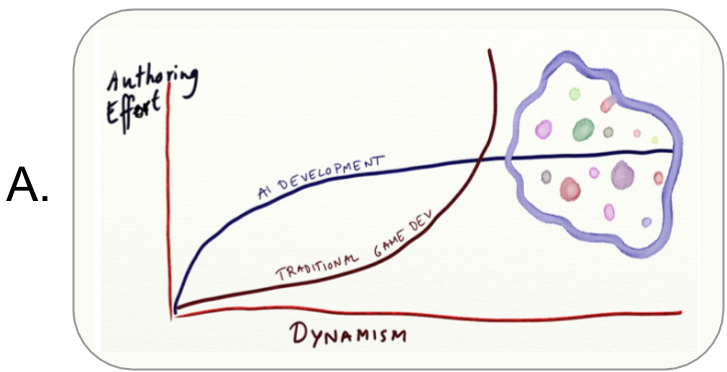
\includegraphics[width=\textwidth]{figures/1A.png}
    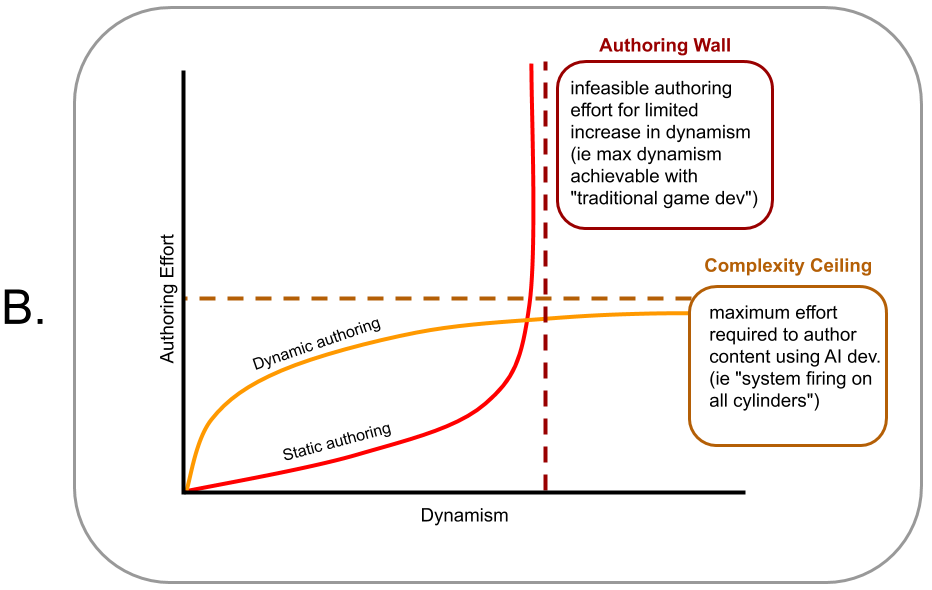
\includegraphics[width=\textwidth]{figures/1B.png}
    \caption{A: Original graph from \cite{mateas2012artificial} As ``traditional game dev approaches" increase dynamism, the authoring effort increases asymptotically. \newline B: Modified graph. The line of dynamism these static systems struggle to pass is the ``authoring wall", which ``AI development" can pass. The level of authoring effort AI dev asymptotically approaches is what could be called the ``complexity ceiling." Systems should seek to lower the ``complexity ceiling" through the use of authoring tools, and pass the authoring wall for a concomitant static system quickly by leaning into the unique affordances of their dynamic system.}
    \label{fig:authoringWall1}
\end{figure}
%%%%%%%%%%%%%%%%%%%% Figure/Image 1 Ends here %%%%%%%%%%%%%%%%%%%%



%%%%%%%%%%%%%%%%%%%% Figure/Image starts here %%%%%%%%%%%%%%%%%%%%
\begin{figure}
    \centering
    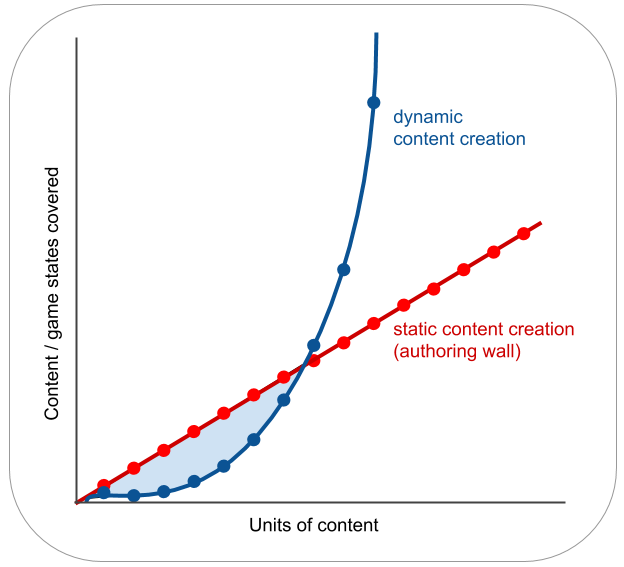
\includegraphics[width=8.5cm]{figures/2.png}
    \caption{Desired performance of dynamic systems when compared to static. While they may underperform initially, their dynamism allows them to cover more states eventually, and the performance gains (hopefully) far outstrip the initial underperformance, enabling new media experiences.}
    \label{fig:authoringWall2}
\end{figure}
%%%%%%%%%%%%%%%%%%%% Figure/Image 1 Ends here %%%%%%%%%%%%%%%%%%%%

These graphs are good at illustrating the interplay between ``effort" and ``dynamism." Another way to look at it is through the lens of content unit production (Figure 2). The authoring wall in this case is the static content creation strategy, which is specific to the system and experience being considered. The static authoring approach always makes incremental progress for each piece of content added, but never sees any increase in game state coverage due to system dynamics. The key interplay here is that, while dynamic systems may require more units of content to initially cover game states (and thus require more effort than static methods) over time that authoring compounds, which allows dynamic systems to exploit those gains to cover more game states than the more ``manual approach" required by static content creation. Ideally, in time the gains made from this ``compounded coverage" outstrip static approaches by so much that they functionally enable new types of media experiences that otherwise wouldn't be possible.

Alternatively, the area below the static version of the authoring wall can also be where the authoring time for a dynamic piece of content fulfilling some number of cases is greater than the time it would take to author enough static content to fulfill the same number of cases. For example, a dynamic unit of content that covers 10 games states but takes an hour to write is ``slower" than 10 units of static content that cover one state per piece and can all be written in half an hour.

Conversely, to be considered past the wall, authoring one piece of dynamic content needs to be either faster, or cover more cases than the time it would take to statically author for the same number of cases.

Regardless which of these two lens is used to view it, overcoming the authoring wall requires careful planning and design. This isn't meant as proscriptive for all dynamic narrative works: too much structure early on may stifle creativity for some practitioners, and the benefits of content planning may not outweigh the loss in creative output in some cases. Similarly, dynamic narrative content may seem like a natural fit for some projects, or a potentially exciting bell-and-whistle, when the reality of the design is one which can be satisfied with static content more reliably. 

However, for some types of dynamisms, systems are necessary to provide the project's required breadth and depth of content reactivity. By extension, leaning into the strengths of said systems when creating dynamic content yields more useful content than what could be obtained through static authoring alone. Furthermore, surfacing the system's capabilities to the player through the content provides a unique affect that can both help guide the player's interactions by signposting the types of interactions it excels at, and better communicate the story it's trying to tell. And for projects looking to keep to a deadline or guard against scope creep, understanding the project's authoring wall is a critical part of the design process.

Critically, where the authoring wall exists is not simply a function of the technical system, but hinges heavily on the narrative design of the experience authored with the system. Generally speaking, if the narrative design of the experience is leaning into the strengths of the system, the authoring wall is passed quicker. And the more dynamic the system and design, in general the further out the wall will be (requiring more authoring up front), but the greater the leverage once you're past the wall. 

Similarly, good design for these dynamic systems should be one where a static version of the same content very quickly becomes infeasible, because that demonstrates that the dynamisms enabled by the system are being exploited successfully to create a unique experience. If far into a project the static authoring method is still providing a competitive solution to that of the system, re-evaluation of the content design should be considered.

And while there is a rich seam of academic research in the creation of dynamic narrative systems and their attendant challenges, too often the concomitant \textit{design} challenges are not addressed or developed with equal footing. These systems may enable amazing interactive experiences, but creating a first-class game or media experience with them is often untenable. Some require incredibly technical skills to create one piece of content, which makes the per-unit time discouragingly high. Some allow fast authoring, but need such a large amount of content that authoring it in necessary volume requires a time commitment that is discouragingly high.

\section*{The Value of Content Creation For Research}

Critically, in these comparisons we are assuming ``surface text quality parity" between static hand-authored content and dynamic content, and that the quality level is that of a fully realized narrative experience. While an argument could be made for sacrificing the quality of content for an exchange in dynamism, in general any provisional authoring not meeting the quality standards for a fully-realized experience is setting itself up for more of a theoretical, research-focused experience creation. Because we are concerned with new forms of interactive narrative that can be experienced as fully realized experiences in their own right, in this dissertation we will be focused on authorial issues as they apply to this goal of polished output, as opposed to more provisional content used in research focused more primarily on system dynamics, with less a mind for what experiences using it might entail.

This focus was chosen because, in our experience, these dynamisms (and their attendant problems) only emerge during authoring of fully realized content, exposing weaknesses or blind spots rooted in assumptions of the underlying system. Because of this, development of dynamic narrative systems can't be considered pragmatically complete until exemplary content is authored with them. Therefore, the development of even theoretical interactive narrative systems can still introduce new concomitant procedural design and content authoring strategies. These strategies, even if unique to their corresponding system, represent paired first-class research contributions.

This stance is one that has been shared by other researchers in the field for quite some time, spurred by calls to make ``this powerful new medium for multiform narrative as expressive of the writer’s voice as is the printed page" \cite[250]{hamlet_holodeck}, concern over the resultant combinatorial explosion such experiences entail \cite{combo_stern}, the need for humanities-style analysis of the media artifacts resulting from such systems \cite{koenitz_five_theses}, and calls for new methods of research evaluation that can take into account the contributions from not just ``demonstrations", but also ``projects" and fully-fledged ``products" \cite[63-64]{wardrip2014envisioning}.

Thus we have narrative systems, which provide grounded solutions to technical problems, paired with content authoring strategies, which provide solutions to the authoring space problem each system poses. Unifying both, and treating the authoring insights as first-class research results alongside the system, allows us to increase the utility of the developed systems, by providing guides for playing to their strengths, and avoiding their particular pitfalls. Furthermore, these authoring insights may be generalizable to other systems, and used to overcome recurring problems when authoring dynamic content.

This position is one which was adopted over the course of six years of research into dynamic narrative systems, paired with media experiences that helped ground them in the pragmatics of content creation. Doing so has brought us up sharply against the Authoring Wall in different contexts, and from the different strategies used to engage and overcome it, the Authorial Leverage framework was abstracted.

\section*{Authorial Leverage}

Broadly speaking, these system-specific design insights have a common goal: maximization of authorial leverage. Thus, having a framework to characterize content creation with high authorial leverage is useful to drive development of the systems, and evolve them further as content is created with them.

Authorial leverage was first formally defined by Chen et al as ``the power a tool gives an author to define a quality interactive experience in line with their goals, relative to the tool’s authorial complexity" \cite{chen2009evaluating}, although previously used by Strong \cite{strong2008talking} to talk about combinatoric authoring, and simply as ``leverage" by Mateas when discussing semiotic systems that facilitate authoring for complex systems \cite{mateas2003expressive}.

For our purposes, it's useful to break down authorial leverage further, and center it on the pragmatics of dynamic narrative production. For ambitious systems with lots of state space and dynamism, greater authorial leverage means both being able to surface that state space to the player, and cover the necessary dynamic points, all without breaking the back of the writers or the project's budget (which effectively translates into labor as well). Knowing what factors play into authorial leverage can help us profile and evaluate system designs, in order to avoid situations where the amount of authoring is infeasible to accomplish the experience's goals.

To this end, we're concerned with two main components of authorial leverage: traversability (which is the scope of the dynamism presented to the player, and how content is deployed to accomplish that) and authorability (the system's requirements for content creation). Each has their own breakdown of important questions necessary to keep in mind when designing dynamic narrative systems.

\subsection{Traversability}

Before we can talk about creating content for an experience, we need to first understand the breadth and depth of what we're trying to achieve. Because this is a pragmatic framework, centered on the experience as the end-goal, our overarching question is: how much of the authored content is seen by the player by the time they have finished playing the game? 

This breaks down into the following four categories of questions:

\begin{itemize}
	\item \textbf{Explorability}: how many content pieces does the player see in one complete playthrough? 
	\item \textbf{Replayability}: how many playthroughs is the player expected to undertake?
	\item \textbf{Reusability}: how many situations could an authored piece of content be reused in different contexts in a playthrough? How many different prospective playthroughs could content reappear in?
	\item \textbf{Contextuality}: how reactive/dependent is the content to player interaction/game state, and how large is that state space? How granular?
\end{itemize}

The answers to these questions determine the scale of the undertaking, the size of the task we're placing before the content authors. We'll now go into each of these in more depth to elaborate their specific concerns.

\subsubsection{Explorability}

When characterizing dynamic narrative experiences (and the authoring issues that accompany them) we need to first think about to what degree they are dynamic. We can make that a player-focused lens by asking instead how much dynamic content the player can explore in a given playthrough. Coupled with multiple playthroughs (which we will cover next in Replayability) we can characterize the amount of dynamism necessary to afford the player adequate material to explore the content appropriately. For example, a choice-based narrative that proceeds forward with no loops has less Explorability than a work in which players can make choices and undo them. Characterizing how much content the player will see in a given playthrough can not only help us focus on what is the ``minimum viable product" for our experience, but can provoke thinking on where to focus authoring effort on more dynamic sections. For example, if the most stripped-down version of the player's experience already seems like an infeasible amount of authorial burden, re-scoping the dynamism to more discrete moments (or shortening the experience in other ways) can allow designers to still leverage the system dynamism, while still being able to create a fully realized experience.

\subsubsection{Replayability}

Explorability can be compounded by Replayability. Experiences that are designed to be replayed several times have different authoring considerations than those that are authored to be generative within a single, explorative playthrough. For example, in many choice-based narratives (dynamic or not) the design of the content is often geared around the player replaying the experience to make different choices, and see their consequences. While the affordance of agency in a choice-based game is still compelling with a single playthrough, experiencing multiple playthroughs to explore different pathways can be a critical focus for authoring concerns. Profiling experiences we want to create in terms of Replayability allows us to focus on how we want to structure them, and what content needs more dynamism to avoid seeming overly static. For example, consider a work with a progression like Figure \ref{fig:simplegraph}, where there is a linear experience with one choice between three options.

%%%%%%%%%%%%%%%%%%%% Figure/Image starts here %%%%%%%%%%%%%%%%%%%%
\begin{figure}
    \centering
    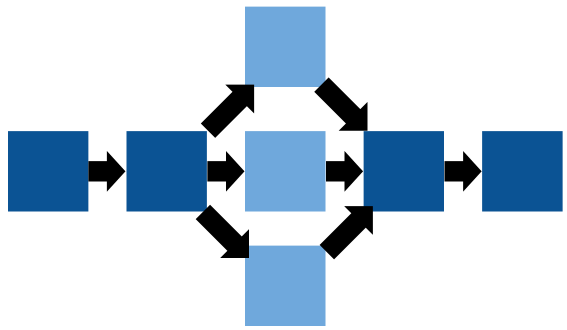
\includegraphics[width=\textwidth]{figures/3.png}
    \caption{A simple linear progression with a choice between three options halfway through.}
    \label{fig:simplegraph}
\end{figure}
%%%%%%%%%%%%%%%%%%%% Figure/Image 1 Ends here %%%%%%%%%%%%%%%%%%%%

If the experience is not designed to be replayed, we can consider each of the beats on a similar authoring level, effort-wise, because the player will encounter any of them a maximum of one time. However, if the work is designed to be heavily replayable, we want to prioritize the dynamism of the dark blue beats, as those are seen many times no matter what choice is picked in the middle. This plays into our next category: Reusability.

\subsubsection{Reusability}

When evaluating a potential experience's system design, we want to characterize how content can be reused, or how often content is common between playthroughs (if Replayability is a factor). As a general consideration, the more content is being reused, the heavier the lifting it's doing. This usually means the process intensity \cite{crawford1987process} will need to be higher, but that the quantity of required authoring (hopefully) is lower. However, the amount of different places content can be successfully reused depends on the work's Contextuality, which works in concert with this lens to either compound the Complexity requirement (as we'll see in Section \ref{sa-reusability} with \textit{Emma's Journey}) or facilitate Reusability if the amount of required Contextuality is relatively low.

\subsubsection{Contextuality}

One of the experience qualities that can impact authoring the most is its Contextuality. This category provides a useful lens for clarifying the relationship between the narrative and the state space of the game. For example, the authoring requirements for a narrative that contextually reacts to--and surfaces--a state-space of five boolean variables is very different from one that does so for fifty. Additionally, a narrative that reacts to game state that updates once a second is very different than one which only reacts once per player interaction, such as clicking a choice. High Contextuality experiences in this sense are more reactive and dynamic, though that dynamism of course comes with an authoring cost.

This lens is also useful for thinking about the dynamic juxtaposition of content for different intended narrative modes. We will explore this more thoroughly later in Section \ref{subsubsec:failbetter-and-qbn-systems} with Failbetter's concept of ``fires in the desert." For now it is enough to say that an experience in which an individual piece of content must make sense and support continuity from a previous one--such as narratives driven mostly by conversations between characters--poses a much higher Contextuality challenge than ones where each individual piece of content is a self-sufficient vignette. While the latter can rely on the player to fill in the context gaps and therefore has more leeway for Reusability, the former has a much higher standard for coherence (a dynamic we will elaborate upon in Section \ref{intro:controllability}) and as such can foreground a high amount of authorial burden.

\subsubsection{Summary}

These lenses help us evaluate a proposed narrative experience in terms of the player experience, with an eye towards clarifying issues that can impact the amount of authoring required to result in a completed media work. In general, the most challenging experiences will be ones in which the Explorability and Replayability of the play experience is high, the Reusability of authored content is low, and the Contextuality of content is high. However, even if the overall Traversability of a proposed experience is very high, it can still be tackled by relatively small teams of writers, given the proper tools and content design. This plays into the second component of the framework: Authorability.

\subsection{Authorability}

For Authorability, the overarching question is: how quickly / easily can content be created for the experience? For greater specificity, we break this down into the following four sub-questions:

\begin{itemize}
    \item \textbf{Proficiency}: what data format are authors required to work in? How technically demanding is that format?
    \item \textbf{Complexity}: how many different components does authoring a single piece of content entail?
    \item \textbf{Clarity}: how complex are the state/system dynamics that need to be kept in mind while authoring?
    \item \textbf{Controllability}: how difficult is it to create content which is reliably displayed in the intended manner when encountered by the player?
\end{itemize}

\subsubsection{Proficiency}

Proficiency is drawn primarily from Shneiderman's concept of ``direct manipulation'' \cite{shneiderman}, a useful lens for talking about authoring challenges for dynamic narrative systems. Essentially, direct manipulation is a goal for interfaces that can be used by novices easily, experts with fluency, and with a tight loop between an action taken in the tool, and its effect. 

Because dynamic narrative creation already requires authors to keep many things in mind (the characters, the story, the aesthetics, the ``possibility space'' of the narrative, all of which we will address shortly) we want to minimize the initial mental overhead for basic system-driven requirements as much as possible. Therefore, a system that has a low Proficiency requirement is desirable, within the restraints and requirements of other project variables. 

This is similar to the conclusion drawn by Spierling and Szilas in 2009, while assisting students authoring content for their dynamic narrative systems \cite{authoring_issues}. An additional note that plays into Proficiency as well, as they detailed, is that there is a ``vicious circle" in authoring for a system under active development. Authors may find they need new affordances in the course of content creation, which provoke changes to the underlying systems by engineers, which can then result in a higher Proficiency requirement, or a substantial change in content authoring that effectively erases any gained Proficiency due to new required syntax to support the added features.

Keeping Proficiency requirements low is particularly challenging with dynamic narrative experiences, because many times (as we'll see in the projects detailed in this dissertation) the surface text authoring needs to incorporate more advanced syntax, such as some sort of DSL (domain-specific language) to allow authors to specify different methods--state-driven or otherwise--the text may be reified and displayed. The design of these DSLs can potentially alleviate this if done with care, but ultimately depends wholly on the targeted Proficiency of the content authors. 

For example, imagine we need to write content for a character leaving a party. As authors, we know there are a couple different ways this can play out. Let's say they can leave amiably or angrily, depending on how well their conversations went. If we wanted to keep the required Proficiency low for authoring this content, we could have the systems person write a function that evaluates the conversations, and applies some formula resulting in ``positive" or ``negative." The author could then write something like \verb!_pn{That was nice.|That was terrible.}!. This sacrifices the author's ability to see or specify the conditions of what is a ``positive" or ``negative" state, for the ability to focus more on the text itself with a minimal amount of markup, and the capability to call that function despite a low Proficiency. If the author has higher Proficiency, we could risk exposing those conditions to them in a more complex DSL, which would give them higher individual authoring affordance, at the expense of requiring higher Proficiency (and higher Complexity, as we'll see in the following section).

\subsubsection{Complexity}

Hutchins et al. elaborated on Shneiderman's concept of direct manipulation as being the result of minimizing the \textit{Gulf of Execution} and the \textit{Gulf of Evaluation} \cite{Hutchins}, which have analogues with our notion of Complexity and Clarity. We use Complexity as a useful lens for characterizing the amount of effort necessary to take an action to achieve an authoring goal. The effort, as it applies to our targeted domain of content authoring, is characterized primarily through the complexity of data input required to create a singular piece of content. This problem is not new. Spierling and Szilas also encountered this with their authoring efforts, noting that ``even with graphical templates that help create the correct syntax, entering data takes time and prevents from quickly seeing the result of the created content" \cite{authoring_issues}.

While increases in Complexity are often unavoidable with increases in system expressiveness, it can be mitigated by proper tooling. Hutchins et al used a notion of \textit{semantic distance} to talk about how proper tools could close the Gulf of Execution: ``Semantic distance in the gulf of execution reflects how much of the required structure is provided by the system and how much by the user. The more that the user must provide, the greater the distance to be bridged" \cite{Hutchins}. 

Authoring tools which can aggregate disparate parts of the authoring process under one unified interface can decrease the semantic distance. For example, if a piece of content requires both surface text to be written, and semantic tagging to be applied to it to be understood by the game's process, one could lower the authoring Complexity by incorporating the authoring of both text and tags into one interface, as opposed to two disjoint ones. Another useful strategy is to incorporate the game's system dynamics such that invalid options cannot be authored, thus also reducing the semantic distance. For example, if a piece of content requires a reference to another piece of content, creating a field which automatically has valid options would decrease complexity, as opposed to requiring authors to look up reference IDs from another file. These HCI concerns can be generalized as a goal of ``making the commands and mechanisms of the system match the thoughts and goals of the user" \cite{Hutchins}. 

In general, we want Complexity to be as low as possible. This can be difficult with interactive narrative systems, because many times surface text authoring engages a different mindset than narrative design considerations of how / when / where said content is displayed. In practice, we can alleviate this by segmenting authoring tasks between the more system dynamics-focused narrative design tasks, and the aesthetic considerations of surface text authoring. However, care must be taken in the segmentation, as the separation of information and context can decrease Clarity for each component task, as we will detail in the following section.

\subsubsection{Clarity}

Paired with Hutchins et al's \textit{Gulf of Execution} is the \textit{Gulf of Evaluation}, which we partially incorporate as part of Clarity, and another part as Controllability (which we will detail in the next section). In general, we want the process-driven mechanics of content surfaced to the author as they're creating content, in as clear a manner as possible. We can do this by creating, as Hutchins et al say, an authoring interface that can ``present a good conceptual model of the system that is readily perceived, interpreted, and evaluated." For the three main projects detailed in this dissertation, this is mostly accomplished through data visualizations, which can place the content in context with playthroughs, or show the percentage of time particular content is displayed, and under what conditions. For works with a high amount of Contextuality, it is especially important that authors have Clarity in order to control how the content pieces are brought into juxtaposition with each other (as expanded in the next section on Controllability). 

For more lower-level concerns of surface text display, Clarity can be generally increased by providing ``live previews" of different ways the text may reify, and provide an easy way to see their expressive breadth. One tool particularly good at this is Compton's Tracery editor \cite{compton2015tracery}, which provides an easy way to specify the number of expansion iterations one wishes to see, and then expand out the authored context-free grammar to surface text. This leads to a tighter loop between evaluating the final text displayed, and the authoring of further dynamisms.

We want Clarity to be as high possible because without it, the link between the content and its dynamics is weakened. Especially for works which we want a high amount of Controllability (which is true of all the works detailed in this dissertation), low Clarity can mean either capitulating with simpler dynamics and conditions driving its display, or the risk of more surprising or uncontrolled juxtapositions, characterized as low Controllability.

\subsubsection{Controllability}
\label{intro:controllability}

Controllability describes how easy it is to create something with bad dynamics, or dynamics resulting in unexpected output. As a lens on Authorability, it's in dialogue with the type of generativity desired for the dynamic narrative. For example, works with higher Contextuality require higher Controllability for their authoring approaches, because the authors wish to achieve specific juxtapositions of content, though those juxapositions may be dynamically determined and generative.

To this end, as a general rule we always desire high Controllability for authoring, though the scale of what is ``high" or ``low" may differ work to work. Works which are more collage-like with lower Contextuality may have tooling support for ``high" levels of Controllability, which may prove inadequately low when applied to other works which demand much higher Contextuality, and thus Controllability.

The specific types of experiences we set out to create with the systems detailed in this dissertation were all ones in which we wanted a high amount of output control. Because of this, we chose symbolic AI approaches (known colloquially as ``good old-fashioned AI" \cite{haugeland1985artificial}). This is in contrast to a class of generative narrative and NLG (natural language generation) approaches which are connectionist, such as those driven by deep learning and machine learning methods \cite{gofai_vs_connectionist_1989}. While a great deal of research effort is rapidly advancing these methods, our emphasis on symbolic systems is motivated primarily by two preferences: syntactic guarantees, and output explainability.

Modern connectivist approaches are certainly generative and expressive, as demonstrated by GPT-2 \cite{radford2019language}, which some practioners have retrained to generate Borgesian wikis of fictional places \cite{book_of_endless_history} and retrained on even smaller corpuses to mimic specific styles, such as Branwen's work with poetry \cite{branwen_2019}. However, there is still a baseline of statistical invariance in the output that we wish to avoid. We want hard guarantees about the system output that is very difficult--if not currently impossible--for these models to provide, while still retaining their expressivity. Even models that ``bake in" control capabilities, such as Keskar et al's CTRL \cite{Keskar2019CTRLAC} (which parameterizes controls for style, content, and task-specific behavior) don't provide the type of fine-grained syntactic control we require for quality guarantees. On a more macro level, we're also focused on works which can maintain and control context over longer instances than a handful of paragraphs, an area that is being actively developed with approaches such as Sparse Transformers \cite{child2019sparsetransformer}, but is still nascent with such types of models.

Additionally, if we used these models and desired to change certain things to affect very specific qualities of specific output, we would run into issues trying to determine what to change in the model to accomplish our goals. While recent advances have been made to crack open the black box of machine learning models through XAI (explainable AI) approaches \cite{gunning2017explainable}, for the most part it is still very difficult to take generated output from these systems, and then come up with concrete steps that can be taken to change their output in highly defined ways.

Thus, while the approaches for the systems in this dissertation are driven by symbolic AI approaches for the abovementioned reasons, the overarching idea of Controllability can map to both symbolic and connectivist ones as well, as a lens to evaluate how rigorously authors must control the output of the system. This translates into higher authoring effort, through the increase in time spent evaluating the conditions that drive content display for the dynamic narrative system, whatever those may be.

\subsubsection{Summary}

The answers to these questions determine the difficulty of the task placed before content creators. If Authorability is low, even small-scale systems may suffer difficulties fielding playable experiences. However, maximizing Authorability by

\begin{itemize}
    \item lowering required Proficiency
    \item reducing authoring Complexity
    \item increasing authorial Clarity while writing for
    \item the level of Controllability appropriate to the experience
\end{itemize}

can help mitigate that. This typically is accomplished through the use of custom editors or other methodologies, and enables more content to be produced. Thus, experiences scoring high in overall Traversability with concomitant high authoring requirements can still be achievably created.

\section*{Related Frameworks}

This framework joins the ranks with other formalizations geared towards aligned but different purposes. Some of them apply to the general domain of game development, others more specifically to narrative games, and others still with content authoring for games.

\subsection{MDA Framework}

In thinking about the dichotomy of content (and its supporting systems) in dialogue with media experience requirements, the Authorial Leverage framework bears similarity to Hunicke and LeBlanc's MDA Framework \cite{hunicke2004mda}. Originally taught in workshops at the Game Developers Conference from 2001-2004 \cite{leblanc_2001}, the MDA Framework ``attempts to bridge the gap between game design and development, game criticism, and technical game research." It breaks down games into three categories: mechanics, dynamics, and aesthetics. Mechanics composes the procedures specifying the ``game-as-system", dynamics the run-time behavior of those procedures, and aesthetics the desired emotional responses evoked by those dynamics. These categories are intended as ``a lens or a view of the game -- separate, but causally linked" \cite{leblanc_2004}. These lenses are then used to inform the iterative design process--to help the game developer ``analyze the \textit{end result} to refine implementation, and analyze the \textit{implementation} to refine the result" \cite{hunicke2004mda}. The Authorial Leverage framework takes a similar tack, where the Traversability questions detailing the desired player experience frame the Authorability questions engaging with the implementation. However, compared to the more abstracted (and thus more generalizable) MDA Framework, the Authorial Leverage Framework is concerned solely with content authoring, and goes into more specific detail profiling how that is to be accomplished.

\subsection{System, Process, Product}

In 2010 Koenitz proposed a framework breaking down interactive dynamic narrative into three components: system, process, and product. Of these components, \textit{system} describes the ``digital artifact, as it exists on a digital storage medium combined with the hardware on which the artifact is executed", \textit{process} the ``actions of the user as interactor, and the opportunities provided by the system define and shape the process", and \textit{product} the completed playthrough produced by the user \cite{koenitz_framework}. This framework was created to find new ways to productively apply narrative theory to interactive digital narratives (abbreviated by Koenitz as IDN). This was motivated by Koenitz's feeling that IDNs are ``participatory transformational experiences", and that there is a key difference between ``the material artifact as a computer program and its output as a particular instantiation." As such, his framework is centered on the distinction between the system (both hardware and software) that enables the playthrough, and the playthrough itself. This is similiar to the Authorial Leverage framework's sub-categories of Explorability, Replayability, and Reusability, as those are similarly motivated to provide a lens to analyze content in terms of potential traversals, rather than a monolithic library.

\subsection{Axes of Analysis}

Three years later in 2013, Koentiz et al incorporated this with even more classification dichotomies, ranging from ``flexible / fixed" to ``script / procedural" and others. The goal of the different classification axes was to promote an analytical framework using ``processes based on small corpora and ad-hoc comparisons between select artifacts to visualize relevant characteristics" \cite{koenitz_idn}. This was in dialogue with previous categorization efforts such as Bevensee et al's PING (Passive-Interactive Narrative-Game) model \cite{aporia}. Bevensee et al created the PING model with its two axis--one for the dichotomy of game versus narrative, the other interactivity versus passivity--to position their work \textit{Aporia}, whose focus is communicating a narrative wholly through environmental storytelling. Koenitz et al's classifications also drew from Bura's proposed dichotomies of ``story versus system" and ``user control versus system control" \cite{koenitz_idn}.

While these types of analytical frameworks are admittedly more ad hoc, they are similarly motivated to the Authorial Leverage framework in that they're focused on providing flexible scaffolds that are based more on the utility they provide for thinking about particular aspects of given works, rather than claiming some sort of objective truth that applies to all dynamic narrative experiences. Additionally, as with PING, the Authorial Leverage framework arose from the abstracted insights derived from implementing specific works, and forming theories based on the experience of authoring with them, that can them be turned to other works to comparatively analyze them.

\subsection{PC3 Framework}

A year later in 2014, Magerko proposed the PC3 Framework, which was motivated by the desire to ``better understand how to dissect, compare, and contrast systems within similar as well as across different presentation media" \cite{magerko_PC3}. The range of ``different presentation media" is quite inclusive, spanning from complex computational narrative systems to simple story card games. The PC3 framework breaks down into the following components:

\begin{itemize}
    \item \textbf{P}: the computational \textit{processes} employed in the work
    \item \textbf{C}: the \textit{content} used in the system (as well as its narrative structure)
    \item \textbf{C}: the system of \textit{control} used to drive content display (centralized or de-centralized)
    \item \textbf{C}: the system's intended social \textit{context} or audience
\end{itemize}

Magerko's abstraction of process to encapsulate both computational and non-computational forms (such as the rules for tabletop games) allows it to juxtapose works that previously may have not been considered comparable. The content and control categories allow it to productively interrogate the surface-level content of works, the dynamics and design in how they are structured, as well as more top-level strategies, such as the use of planners (centralized control) or improv game rules (de-centralized). Lastly, the social context provides a way for the framework to account for the difference in audience for the completed experience. Magerko draws a distinction between the creation of works for training purposes, theatrical performances, or even between children and adults. This grounds the analysis in the pragmatics of its experience, much like the ``Product" in the System, Process, Product framework, or the Aesthetics of the MDA Framework.

PC3 and the Authorial Framework overlap in a few particular ways, although their ultimate aims are different. As with the System, Process, Product Framework, we find it useful to characterize the player's experience as a critical consideration in the system design. And certainly, both frameworks are concerned with dynamic content, and accounting for the dynamics their paired narrative structures entail. However, our Authorability Framework is geared more towards assisting the creators of said systems by providing a lens for strategic authoring decisions. In contrast, the PC3 Framework's focus is more for use by ``teachers, designers, and media theorists interested in the overlap between narrative systems (e.g. identifying the similarities and differences between the narrative systems behind Fiasco, Fa{\c c}ade and Dungeons \& Dragons)" \cite{magerko_PC3}.

\subsection{Progression Model}

New frameworks are continually being created, providing ever more tools for designers and theoriests to analyze interactive narrative works. In 2019, Carstensdottir et al proposed a ``descriptive framework developed to provide designers and practitioners with a common lexicon to describe and analyze their interactive narratives in terms of broad categories of elements that make up the interaction design" \cite{carstensdottir}. This model was derived from analysis of twenty-two games for their structure, progression mechanics, interaction modalities, and presentation. It is interesting to note that, with the exception of \textit{Prom Week} and \textit{Façade}, all were (to this author's knowledge) created by independent or AAA commercial game developers primarily with the singular goal of presenting a polished narrative experience, with no added research goals. Thus, Carstensdottir's model has its roots entirely in works motivated by a polished final experience. In the course of this analysis, Carstensdottir et al also formalized several authoring patterns in the work that they felt could be generalizable to other narrative forms.

Carstensdottir later developed this framework further into their Progression Model, which ``captures the narrative's structure from a users’ experience perspective", with a particular focus on capturing player progression in a graph-based representation called Progression Maps \cite{carstensdottir_diss}. In it, they identified five conceptual categories for interactive narrative design:

\begin{itemize}
    \item \textbf{Structure}: the typical graph-based representation of story progression
    \item \textbf{Progression Mechanics}: mechanics targeted towards player progression through the story
    \item \textbf{Interaction}: player affordance (such as input mapping and feedback)
    \item \textbf{Presentation}: narrative framing such that it impacts player interaction
    \item \textbf{Action Set}: the set of actions available to the player
\end{itemize}

This framework provides a valuable lens to analyze interactive narratives in terms of the user experience, which we are similarly interested in for determining a work's Traversability. However, our focus frames the player's affordance as the instigation point for authorial concerns, and our questions of Authorability, while informed by these questions of player affordance and game traversal, are meant more as a lens for practitioners to use in the course of creating new works.

\section{Contributions}

This dissertation contributes a new framework, the Authorial Leverage Framework, as an abstracted guide for analyzing dynamic narrative experiences (whether in progress or completed) and constructively talking about the authorial burden of their content creation. This framework also enables discussion about sustainably lowering the labor of such works while still preserving desired characteristics. This framework was abstracted from lessons learned in the implementation of three unique dynamic narrative systems, each of which tackles dynamic narrative in a categorically different way.

\begin{enumerate}
    \item \textbf{\textit{Ice-Bound}} creates dynamic narrative the player can sculpt until they arrive at a story of their choosing, through the unique affordances of a combinatorial narrative system.
    \item \textbf{StoryAssembler} marries a forward-search planner approach with a hierarchical task network (HTN) planner to afford greater flexibility in each individual unit of content, used to construct dynamic choice-based narratives.
    \item \textbf{\textit{Delve}} uses hierarchical ``story-sifting" to generate character narratives, and content-tagging coupled with an ontology to enable story manipulation through 3D objects in a first-person game.
\end{enumerate}

Each of these systems provides unique technical insights in their implementation. Furthermore, the process of authoring completed works with them (or in the case of \textit{Delve}, initial tool design to allow such authoring in the future) critically provided design insights that led to both authoring patterns which may be generalizable to other such dynamic systems, and methodologies for determining ``problem spots" in content dynamics, and how to avoid them. Critically, these insights could not have arisen from pure system implementation, only from the pragmatics of experience creation. Said insights are generalized into the Authorial Leverage Framework to facilitate content authoring, and will hopefully provide a useful lens to evaluate the development and design of future procedural narrative systems for others.

\section{Outline}
%%signposting%%
This dissertation explores three ``families" of dynamic narrative systems, through the implementation and content creation process for three separate projects: \textit{Ice-Bound}, \textit{Emma's Journey} (using the StoryAssembler system), and \textit{Delve}. For each, we first foreground the ``experience challenge" that we hoped to answer with said system. Prior works in a similar vein are then profiled, along with a targeted literature review for each system's area of research. For \textit{Ice-Bound}, this is combinatorial narrative. For StoryAssembler the focus is planner-driven systems and dynamic choice-based narrative systems. For \textit{Delve}, we turn to simulation narrativisation systems, computational metaphor systems, and ontology-driven systems. After laying this groundwork, we then dive into the technical details of each system's implementation, and content authoring procedures. 

Having established this, we then analyze each system and authoring approach in terms of the Authorial Leverage framework. We look at both content design decisions used to maximize each system's effectiveness, as well as authoring insights that may generalize to other systems in each family of experiences. Broadly speaking, \textit{Ice-Bound} shows how increasing Clarity is particularly useful for systems with high degrees of Explorability. For StoryAssembler, we focus on how works with high Contextuality require high Controllability, which can create authoring challenges, as seen in \textit{Emma's Journey}. 

Both \textit{Ice-Bound} and \textit{Emma's Journey} are completed experiences. For the last work, \textit{Delve}, we apply the framework to a work for which the systems are completed, but authoring has yet to begin in earnest. Through this, we show how a prospective application of the framework can provide useful guidance for maximizing authorial leverage while iterating on the system, and strategies to fall back on if it turns out the system requirements demand more authoring than we can feasibly provide. We then conclude with some overarching thoughts on the authoring experience across these three systems, and talk about future work in this area.
%%signposting%%
\chapter{Ice-Bound}
%\section{section} (h2)
%\subsection{subsection} (h3)
%\subsubsection{subsubsection} (h4)
%\paragraph{paragraph} (h5)
%\subparagraph{subparagraph}

\textit{Ice-Bound}'s system is a custom combinatorial narrative engine co-created with Aaron Reed, culminating in the release of an indie game in 2014. It's a good case study of an exploratory generative narrative system taken all the way from theoretical implementation to exemplary media experience. \textit{Ice-Bound} won the award for Best Story / World at IndieCade 2014, in addition to being featured in the Independent Games Festival and SXSW.

%%signposting%%
We'll start with detailing the specific experience we were trying to create: an interactive narrative where players can sculpt the story to explore it, through the use of combinatorics. Then, some related systems and works in the area of combinatorial narrative will be explored in Section \ref{sec:ib-related-works}. Thus contextualized, we'll then do a deep dive into \textit{Ice-Bound}'s system specifics in Section \ref{subsec:ice-bound-summary}. This will lead to our application of the Authorial Leverage Framework. First, we will profile the Traversability challenge of the work (driven by the combinatorics and large state space) in Section \ref{subsec:icebound-traversability}. Then in Section \ref{subsec:icebound-authorability} we'll show how that challenge was answered, in this case primarily through focusing on authorial Clarity and increasing that through authoring tools.
%%signposting%%

\section{Experience Challenge}\label{sec:ib-experience-challenge}

\textit{Ice-Bound} conceptually started as a pitched project for the ``Envisioning the Future of the Book" grant from the Center for Book and Paper Arts at Columbia College Chicago. This grant was looking for works that could ``take both virtual and physical manifestations, examining the advantages of each and how the interplay between the two can be leveraged to provide a comprehensive and powerful expression" \cite{rhizome_2012}. Specifically, they were looking for physical artists' books that would exist in dialogue with a digital system.

We took the prompt of what the ``future of books" would be, and extrapolated it out (somewhat facetiously) to ``what use are physical books in a future where all books are digital?" The seed that would grow to be our core story came from a sardonic answer: DRM (digital rights management).

For \textit{Ice-Bound}, there are two components. A physical printed book, \textit{The Ice-Bound Compendium}, and the digital game: \textit{The Ice-Bound Concordance}. The frame narrative of the work positions it in the future, where the primary reason for printed books' existence is that human-level AIs cannot easily access their information. The \textit{Compendium}, therefore, is a collection of secret materials and ``transmissions" about the main character of the work, Kris Homquist (or as his AI simulacrum is known: KRIS). It was put in print form to prevent him from being able to access it, as a simulacrum can easily access all digital information, but can be easily prevented from accessing the physical world.

The character you interact with, KRIS, is an AI created from a brain scan of Kris Holmquist, a popular writer. Kris died before he could finish his masterpiece \textit{Ice-Bound}, and because he was under contract with a publisher for it, they decided to ``spin up" a copy of him to finish it. Unfortunately, the personal issues that hounded Kris make it impossible for KRIS to finish the work, or decide what is the best way for the story to go (in a very ``life imitates art" manner). The player, in this case, is ``assigned" to KRIS to help shepherd him through the editing process, deciding which of the many ways the story can go is the ``correct one", and in the course of that, forcing him to confront the past mistakes and issues of his life that kept him from finishing his magnum opus.

That is a very linear and simplified version of the story, of course. The book material is meant to interface with the digital game in a collage-like and orderless manner--there is no correct order to read the \textit{Compendium} in, and no guarantee that a certain section of the story will be seen before another. It is meant to be taken in as a sort of ``narrative possibility space" whose details are teased out by determining where the voices are in chorus, not in discord.

While we did not receive that particular grant, we came away from it with a solid project proposal. When another grant--UCSC's SPIN (Student Project INcubator) Studio grant--became available, we used that application process to expand upon the proposal with a digital prototype.

%%%%%%%% BEGIN FIGURE %%%%%%%%%%%%%%%%%%%%%%%%%%%%%%%%%

\begin{figure}
    \centering
    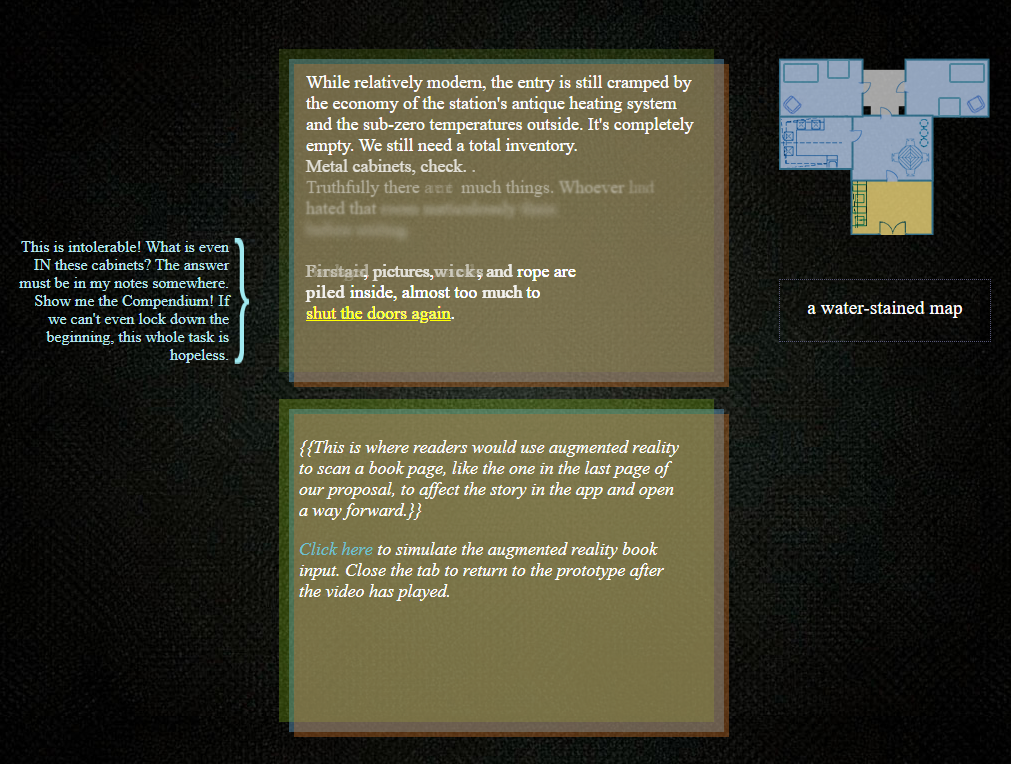
\includegraphics[width=\textwidth]{figures/2-Ice-Bound/digital-prototype.png}
    \caption{Early, non-combinatorial prototype of \textit{Ice-Bound}.}
    \label{fig:digital-prototype}
\end{figure}

%%%%%%%%%%%% END FIGURE %%%%%%%%%%%%%%%%%%%%%%%%%%%%%%%%

The initial prototype was much closer to a visual interface for a traditional text game as its central metaphor (Figure \ref{fig:digital-prototype}). We thought we would create a game in which players moved through rooms, casting ``light" on them as they moved, which would allow them to interact with the different objects within. Moving the objects to different rooms would unlock different capabilities, and change the story told on that level. This was much closer to a ``lock and key" system than a combinatoric one, although the potential for different objects in each room was the seed of the combinatorics we'd later embrace.

We still had unresolved questions about what such a design would require authoring-wise, but we knew that undertaking a dynamic narrative project could easily result in untenable authorial burden if we weren't conscious of our content creation commitments at all times of the design process.

Initially, we flirted with the idea of using Skald---Tearse's reconstruction of Turner's Minstrel system \cite{tearse_skald}---to generate narratives. Aaron Reed, the project's co-creator, had done some work with the system and had a good working understanding of it. But we dropped that early on in order to create a more bespoke system that would speak to the particular strengths targeted for our project, and whose capabilities could evolve as the design itself evolved.
%%GDoc comments%%
Before we began in earnest on the digital system design, we went through a period of paper prototyping to shed light on the types of dynamics that would emerge from the kind of interactions we wanted to foster for our target experience. This practice is well known in HCI (Human Computer Interaction) circles colloquially as the ``Wizard of Oz" technique or Oz technique, which has been around since 1975 where it was first known as the ``experimenter in the loop technique" \cite{wizard_of_oz}. Some of its first uses were in iterative prototypes of natural-language interfaces, where the experimenter would manually type out dictation spoken by the subject. As development continued, the ``wizard" became less necessary, until ultimately the program could run without intervention \cite{kelley1984iterative}. Since then, it has been used as a useful way to quickly iterate on graphical interfaces \cite{snyder2003paper} and game mechanics \cite{mayra2004player} as well as generative narrative systems \cite{cozy_mystery}.
%%GDoc comments%%
Once we began paper prototyping, it became quickly apparent that in order to control authoring burden, we would need a way to flexibly limit or group story components to reduce combinatorics where necessary. We found we could successfully gauge this by using small cards with sections of story on them, then having one person be ``the player" and ``activate" different parts of the story, while the other person played ``the computer", and used different types of rules to determine what to display to the player.

%%%%%%%% BEGIN FIGURE %%%%%%%%%%%%%%%%%%%%%%%%%%%%%%%%%

\begin{figure}
    \centering
    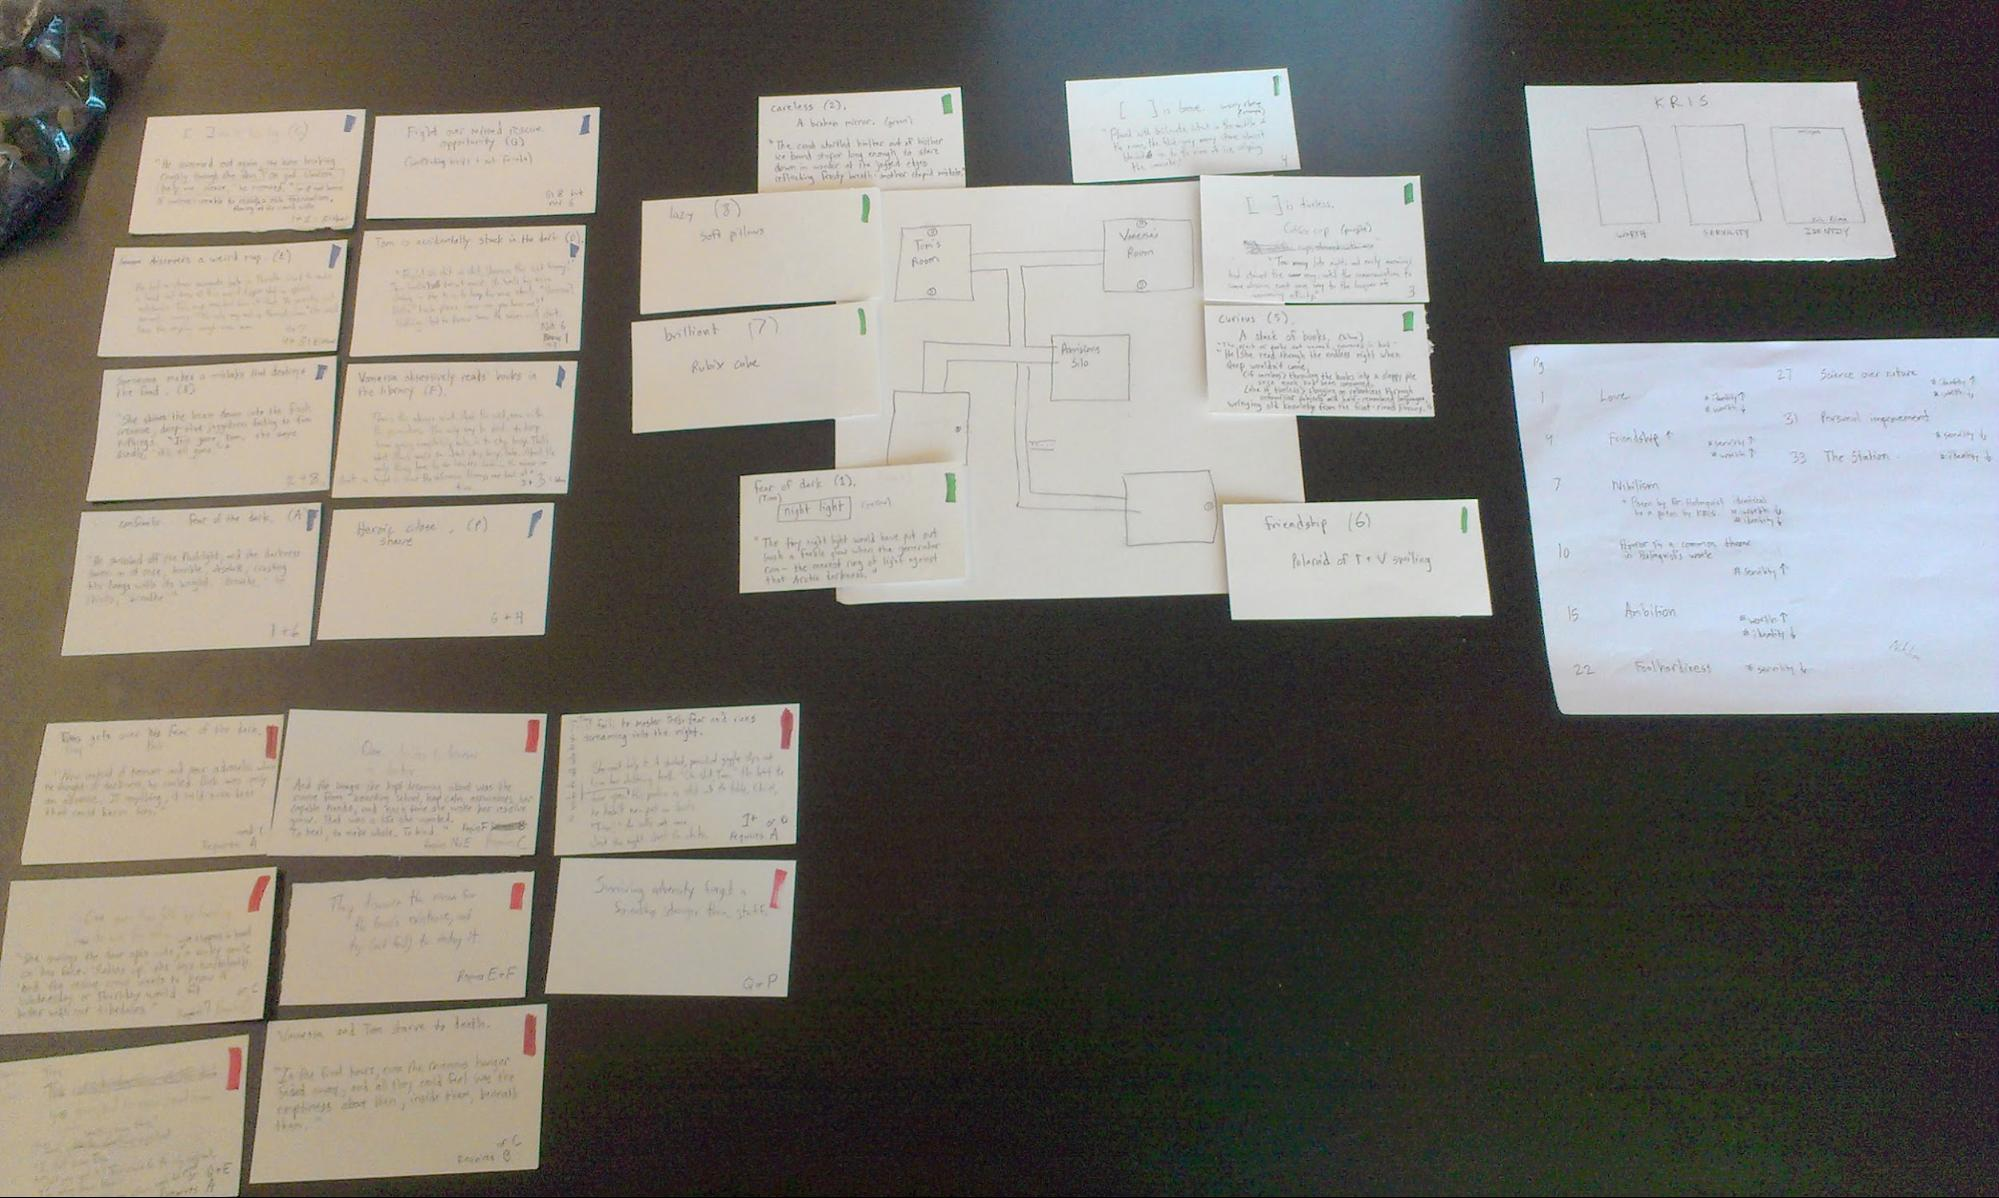
\includegraphics[width=\textwidth]{figures/2-Ice-Bound/prototype.jpg}
    \caption{Early paper prototype of \textit{Ice-Bound}, showing symbol, event, and ending cards, along with a map. The ``player" would choose symbol cards to flip over on the map, and the ``computer" would then consult the deck of events and endings, and flip over the corresponding ones.}
    \label{fig:prototype}
\end{figure}

%%%%%%%%%%%% END FIGURE %%%%%%%%%%%%%%%%%%%%%%%%%%%%%%%%

From there, we would loosen or constrain the pre-conditions on cards, coming up with new categories of pre-conditions when necessary, while also keeping an eye on how many cards we were setting ourselves up to write to fulfill all the combinations. This design process of refining the system, then refining the type of experience to provide to lean into those strengths, then refining the system further to support aspects we discovered we really needed, was very productive.

After this exploratory period of paper prototyping and iterating, we determined the two pillars of our experience were high quality hand-authored text that one would normally see in static branching narratives, but with a kind of responsiveness and granularity that would encourage exploration and playfulness with the materials of the story.

Aaron Reed detailed this best in his post-mortem \cite{reed2014ice}:

\begin{quote}
We wanted to find a core mechanic that gave us the best of both approaches: the focused, quality surface text offered by branching paths, with the sense of playful exploration allowed by simulationist works [...] one author proposed the notion of "sculptural fiction" to identify works that involve frequent small but reversible decisions, to create a play aesthetic closer to a sculptor constantly refining a work than a rat navigating a maze. The focus should be on continuous, small, reversible choices, creating a playful and exploratory feel.
\end{quote}

This, combined with longer form, static materials in the \textit{Compendium}, would allow us to tell a story that was finely crafted yet interactive, and give the player a sense that they had a real hand in helping KRIS find the perfect ending to his magnum opus.

Our hope was to create an experience where the player could craft a story they felt ownership over, and felt it was happening in the context of a very dynamic and responsive system, but would never feel that the text of the story they were creating was ``stubbed in" or meant to only represent the plot outline or summary of the story. We didn't want the player's experience of the system to be one where the system itself was foregrounded, with the story as accompaniment. Rather, we wanted more of a collage narrative that would still elide certain connective parts of the story (which was necessary, in order to keep technical commitments reasonable) but would do so in a stylistic way that would allow the project to stand not just on the technological merits of its generative system, but the artistic merits of the story it told.

\section{Related Works}\label{sec:ib-related-works}
%%GDoc comments%%
Combinatorial narrative---as a broad category of experiences---has a long history in works both digital and analog. To give a general sense of the space and how it relates to \textit{Ice-Bound}, we'll look first at non-digital forms of combinatorial fiction, then more modern digital incarnations in the form of games. These works were not only guiding contexts for \textit{Ice-Bound}'s system implementation, but also in the aesthetic quality of story such systems facilitate, as an inspiration for \textit{Ice-Bound}'s fiction.
%%GDoc comments%%
\subsection{Non-Digital Combinatorial Fiction}\label{subsec:ib-non-digital-combinatorial}

Digital combinatorial fiction is embedded in a much longer non-digital tradition extending back through Oulipean constrained writing works and beyond. An exhaustive survey is outside the scope of this dissertation, but there are a selection of works that provide an interesting lens into this large and varied body of literature.

\subsubsection{Oulipo and Shuffle Literature}\label{subsubsec:oulipo-and-shuffle-literature}

Experiments with combinatorics have bridged both prose and poetry. Raymond Queneau's \textit{Cent mille milliards de poèmes} \cite{mille_poems} is positioned at the genesis of the Oulipo movement in 1960, being ten sonnets, of which each line can be swapped between each sonnet. The combinatorics of this give the collection its title, and served as an initial sort of ``flag-planting" for the project of this influential group. This area of combinatorial work also has partnership with the sciences at its roots. After completing only half the sonnets, Queneau wrote that he lacked the ``courage to continue", due to the increasing difficulty of composing the sonnets in a ``natural voice" as the potential combinations increased. It was only after consulting with François Le Lionnais---a scientist and mathematician by trade---that he was spurred to overcome his reservations \cite{audiberti_charbonnier_1965}. It was from this first partnership that Oulipo sprung.

The notion of works which can communicate a narrative or poetic experience no matter the order their composite pieces are read in is an idea that beguiled many experimental writers. Montfort and Husárová proposed a useful category for these works as ``shuffle literature", and that the discursive project of this approach is to ``rearrange the discourse and model processes of memory, random association, and cognition", while still evoking many of the traditional aspects of bound books \cite{shuffle_2012}. The works span from Saporta's \textit{Composition No. 1} \cite{saporta1963composition}---a 1962 detective novel which requires the pages to be shuffled before being read---to the more modern \textit{Heart Suit} by Robert Coover \cite{coover2005heart}, a 2005 story published on thirteen playing cards which can be read in any order, each card ending mid-sentence with ellipses. 

Because it is such a considerable constraint to write in such a manner, usually the form chosen for these works contains meaning which enriches the work. For example, in a similarly card-based work \textit{The Family Arcana}---which uses a full poker deck of cards---the suits and face cards correspond to which characters are the subject \cite{short_card_deck}.

There's a general distinction one could make about these types of works, which stands somewhat in contrast to the digital systems we will soon visit in Section \ref{subsec:digital-combinatorial-fiction}. In terms of the story they hope to tell, the combinatorial nature of it is given more as an expressive affordance for a unified area of narrative possibility, as opposed to giving the reader agency to take action to drive the plot, such as in \textit{Choose Your Own Adventure} style works. Montfort and Husárová posit that in shuffle literature, ``The reader has not been given the power of the heavy hand of fate, the capability to influence events, but by being given a hand of events, recollections, and moments, the reader is invited to feel how they can be sorted, recalled, and told in different ways" \cite{shuffle_2012}. And many of the writers support this interpretation. In an interview, B.S. Johnson---writer of the 1969 shuffle literature work \textit{The Unfortunates}---said that his pursuit of portraying the ``simultaneity and multiplicity of modern life" was a problem that combinatorial approaches help solve, and that ``it was still a better solution to the problem of conveying the mind’s randomness than the imposed order of a bound book" (quoted in \cite{coe_2002}). Grenier, whose 1978 work Sentences was similarly card-based, said that the connective tissue of relation wasn't something put into the work, but left to the reader, which ``has something to do with fiction, something to do with imagining how something can be" (quoted in \cite{shuffle_2012}).

One of the pernicious problems (though perhaps it could be seen as an artistic choice or affordance) of shuffle literature works comes from the constraint they've set the author: write lexemes (units of text) which can be compelling no matter what order they're read in. The process for these works---simple random selection---makes this exceedingly difficult to guarantee plot or development of certain themes. Some authors get around this by using the combinatorial qualities to communicate different viewpoints of a set plot, so that there is no guarantee of what perspective the reader will get, but guarantees can be made of what the story is about, if they read through enough combinations.

This sort of generativity, while exciting in its promise of variation, foregrounds a secondary issue that has dogged both digital procedural narrative and even procedural generation games in modern times. Jacques Roubau, contemporary procedural poet and early Oulipo member, wrote that Queneau's \textit{Cent mille milliards de poèmes}' ``constraint is rather elementary, but its potentiality is spectacular [...] a work of propaganda in favor of potentiality, much more than it is praise by way of example for writing under constraint" \cite{Roubau}. One can easily find echoes of this exact critique in modern procedural content generation works that struggle with novelty and meaningful content, perhaps loudest in recent memory with the popular digital game \textit{No Man's Sky}, which launched with the boast of containing ``18 quintillion planets." One critic's reply was that the game experience was ``Like 18 Quintillion Bowls of Oatmeal", citing a potent metaphor from Compton on the struggle for meaningful novelty in procedural generation \cite{maiberg_2016}.

This combinatorial approach is the most simple, and least systemic. However, it shows us how compelling works can still be created that communicate particular discursive aesthetics that can't be easily accomplished with static forms. It's important to understand these aesthetic affordances, because before even applying systems to create narratives within them, one should be aware of the baseline acting as a substrate for those efforts.

Additionally however, works can engage with structure through the addition of further constraints to further complexify their generativity, as seen in the following works.

\subsubsection{Castles and Constraints}\label{subsubsec:castles-and-constraints}

Other works were created in this time period that engaged with simple rules and constraints to provide an interesting framing for their narratives. Cortazar's 1963 novel \textit{Rayuela} \cite{cortazar1996rayuela} was designed to be read sequentially, or by ``hopscotching" (from whence it derives its title) through the book using rules laid out in the introduction. Later, a more complex application of systemic constraints through movement was completed by Perec through the use of ``bi-squares": tables used to exhaustively combine separate lists of elements. 

Perec's 1978 work \textit{Life: A User's Manual}, a novel about a Parisian apartment block, took 42 lists of qualities (each with ten elements) and organized them into 21 bi-squares. The resulting combinations were distributed across the 99 chapters of the book. Thus, a cell on the 10x10 map of the apartment block contains a corresponding list of element lists, which were used to constrain the chapters \cite{bellos2010georges}.

%%%%%%%% BEGIN FIGURE %%%%%%%%%%%%%%%%%%%%%%%%%%%%%%%%%

\begin{figure}
    \centering
    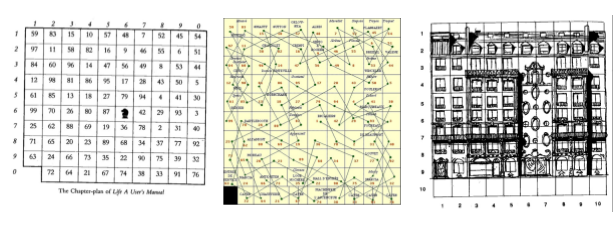
\includegraphics[width=\textwidth]{figures/2-Ice-Bound/calvino-tables.png}
    \caption{The numbered chapters of \textit{Life: A User's Manual} laid out on a grid (left) and the path of the ``knight's tour" comprising their traversal (middle) which describes the story that takes place in the corresponding room in the layout (right) \cite{harding_2014}.}
    \label{fig:calvino-tables}
\end{figure}

%%%%%%%%%%%% END FIGURE %%%%%%%%%%%%%%%%%%%%%%%%%%%%%%%%

Perec then used a ``knight's tour" to traverse the map he had created, a concept that was in vogue within Oulipo at the time. A knight's tour is the path created by moving a knight through a grid while visiting every square (Figure \ref{fig:calvino-tables}). This elaborate system of constraints was created to provide lists of required elements for each chapter. Much like the authoring constraints set up by \textit{Ice-Bound}'s system (whose pragmatics we'll explore in Section \ref{par:pragmatic-tables}), the organization of the thematic system constrains enough that it can actually drive authoring in well-specified ways, though the task may be daunting both in scope, and in the ambitiousness of the coherency of output.

A particularly evocative example of this problem can be seen from Calvino---another Oulipo member---and his engagement with constraint-driven combinatorics. Specifically, his 1973 book \textit{The Castle of Crossed Destinies} engages with a tarot deck to structurally frame two collections of stories \cite{crossed_destinies}. In it he lays out two ``spreads" in the shape of the castle and the tavern, and the vignettes that proceed from the lines of cards are closely tied to the symbols of the cards (Figure \ref{fig:calvino-castle})

%%%%%%%% BEGIN FIGURE %%%%%%%%%%%%%%%%%%%%%%%%%%%%%%%%%

\begin{figure}
    \centering
    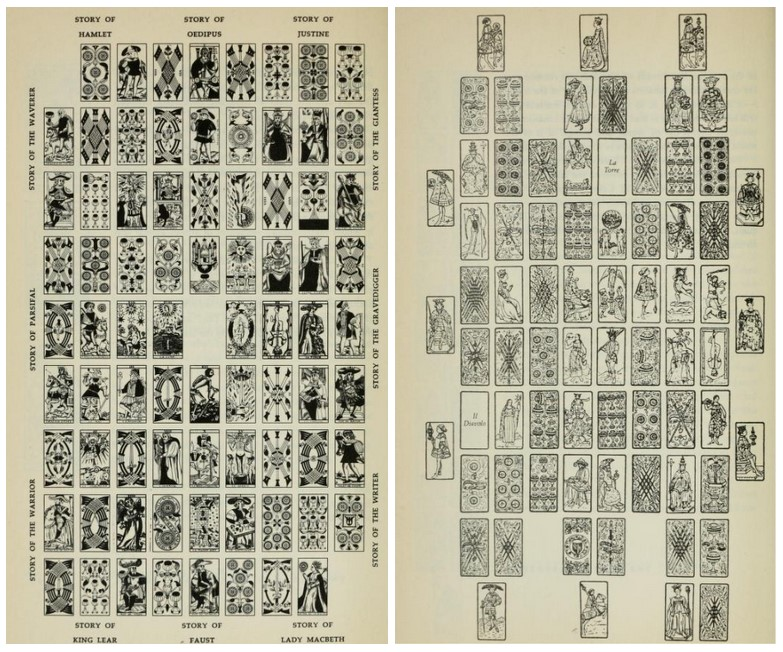
\includegraphics[width=\textwidth]{figures/2-Ice-Bound/castle-of-destinies.jpg}
    \caption{The card layouts for the castle (left) and the tavern (right).}
    \label{fig:calvino-castle}
\end{figure}

%%%%%%%%%%%% END FIGURE %%%%%%%%%%%%%%%%%%%%%%%%%%%%%%%%


While his goal was initially ambitious, the writing of this work proved too daunting and difficult to complete in its purely generative form (accounting for every combination of cards in the layout, with a coherent story for each). Calvino elaborates upon this in the Afterword, where he describes his process: ``I publish this book to be free of it: it has obsessed me for years. I began by trying to line up tarots at random to see if I could read a story in them [...] I looked for other combinations of the same cards; I realized the tarots were a machine for constructing stories." Having realized the generative storytelling potential of the divination deck, potentially ripe with rich and variegated meaning, Calvino was then ``tempted by the diabolical idea of conjuring up all the stories that could be contained in a tarot deck [...] I wanted each of the stories to have a coherent significance."

Calvino's strategies to navigate the generative chaos of combinatorics mirror those used by authors in digital forms. His first approach was to take two existing and well-defined stories---that of \textit{Roland the knight} and \textit{Astolpho}---and pick the tarot cards that would allow him to tell those stories. The rest of the cards he let fall where they may, and told those stories ``as they came." By giving two stories primacy, he was able to chart an easier course through the generative waters, and could excuse discrepancies in the other stories as vagaries of what was necessary to provide the unified structure for the main narratives. He ran into issues however, when---girded perhaps by his success with the tavern section---he was ``unwilling to sacrifice any of the narrative possibilities" for the castle section, and sought something more generative. Practitioners in the field will be well familiar with what resulted: Calvino bemoans how he ``spent whole days taking apart and putting back together my puzzle [...] I drew hundreds of patterns [...] but some essential cards were always left out, and some superfluous ones were always there in the midst. The patterns became so complicated [...] that I myself was lost in them." To escape from this impasse he quite literally gave up on the patterns and instead wrote directly the ``tales that had already taken shape, not concerning myself with whether or not they would find a place in the network of the others." But he was stuck between a rock and a hard place, because without the restraint of the deck, the point of the exercise would be lost. As he says: ``without it, the whole thing was gratuitous."

Calvino also ran into issues with realizing his ``surface text", another familiar problem to practitioners. Though he would successfully come up with a series of cards to use for a story visually, when he began writing them down they would lose their compellingness, and had to be eliminated ``because they would have lowered the tension of the style."

He gave up multiple times, and would then take up the project again later, hoping that a fresh attack ``in a different way, more simple and rapid" would garner success. He spent countless hours shifting and re-aligning symbolic patterns, only to---upon waking the next morning---``tear it up." He never reached a sense of closure with the manuscript, working it over and reformulating it even as the manuscript was in the final stages of publication \cite{crossed_destinies}.

As with previous works we covered, he reflected this dilemma diegetically, such as in The Waverer's Tale, where the Devil card confronts the Waverer and proclaims ``Whoever retraces the way of divided things encounters me, whoever descends to the bottom of contradictions runs into me, whoever mingles again what was separated feels my membraned wing brush his cheek." Also present on the card are two smaller figures on leashes, and Calvino muses that ``it is likewise probably that each of them holds on a leash two other, smaller devils that have remained outside the picture, so that from branch to branch stretches a network of ropes which the wind sways like a great cobweb." A web which resembles the net of correspondances he himself was trapped by in writing the book, although some \cite{conte_1994} have also theorized it was meant to symbolize Borges and his engagement with multiplicity in ``The Garden of Forking Paths."

Calvino set himself a more structured---and therefore perhaps more achievable---goal in 1983 with the novel \textit{Mr. Palomar} \cite{calvino1985mister}. Each section of this work is guided by the constrained combinatorics of three themes partnered with ``kinds of text experience":

\begin{enumerate}
\item Visual (text as pure description)
\item Anthropological / cultural, involving language, meaning, and symbols (text as story)
\item Speculative, concerning cosmos, time, infinity, and the dimensions of the mind (text as  meditation)
\end{enumerate}

The novel is divided up into twenty-seven sections grouped in three levels, each numbered from 1.1.1 to 3.3.3 with every permutation in-between. Therefore, section 1.2.3 would contain an element from each theme/mode category, whereas section 2.3.3 would be lacking in purely descriptive text.

These works, and the thematically constrained writing they provoked, is evocative of the process used for \textit{Ice-Bound}, though our computational processes were more complex. In \textit{Ice-Bound} we determined through early design sessions and testing to use 25 themes (which run the gamut from genre to character traits) for the sake of combinatorics. The ``exercise" of fulfilling the content requirement for that system led us to authoring situations where we would need to write a section with a general mood of horror, with the subject of ``lightning doesn't strike twice," a combination of constraints that perhaps would be familiar to Perec or Calvino. We will revisit and elaborate upon this correspondance in Section \ref{subsubsec:25-themes-and-12-tags}.
%%GDoc comments%%  
% I've now broken these into "non-digital" and "digital" combinatoric works, and expanded the non-digital ones more extensively, while also adding some new sections under the digital works to flesh them out
\subsection{Digital Combinatorial Fiction}\label{subsec:digital-combinatorial-fiction}

Combinatorial narrative really shines, however, when it uses the affordances opened up by computers. Works which normally would be challenging to print or reprint can be translated with ease, such as J.M. Coetzee's digital version of Beckett's \textit{Sans / Lessness} short story consisting of 120 randomly selected sentences \cite{lessness}. But the real benefit comes from the increase in sheer scope computational media affords new works. While enumerating the full breadth and depth of work in digital combinatorial fiction is far beyond the scope of this dissertation, there are some specific categories of works which relate more directly to the specific concerns we had while creating \textit{Ice-Bound}.

\subsubsection{Digital Cards}\label{subsubsec:digital-cards}

One of the most directly related categories of work to \textit{Ice-Bound} revolves around the idea of ``digital cards" as an organizational metaphor. This idea has been around for some time, with a prominent early work being Bernstein's \textit{Card Shark} system which was proposed in 2001 \cite{bernstein_cardshark}. \textit{Card Shark} was a system created to explore the notion of sculptural hypertext, a term Bernstein defined as hyperfiction that is structured ``by removing unwanted connections, much as a sculptor may create objects by removing unwanted material" \cite{bernstein_cardshark}. This was in contrast to what he termed calligraphic hypertext, which begins without links, which the author then creates \cite{bernstein_2007}.This system was not fully developed and used to author works on its own, however the notion of sculptural hypertext was incorporated into StorySpace 3, as an improved authorial affordance on the existing ``guard fields" capability. The ability to add guard fields to lexia is a feature present in StorySpace since its initial versions, as preconditions that could be associated with links between texts. The new functionality added the ability to guard story spaces comprised of several lexia with predicates (called requirements) which could also change the state of the hypertext when certain lexia were visited \cite{bernstein_decline}. This was then used to author a work \textit{Decline and Fall}, to demonstrate the new affordances.

Tarot cards, which so perniciously snared Calvino, have continued to capture the imagination of digital practitioners. Works like Hooper and Weal's 2005 \textit{StorySpinner} system \cite{storyspinner}, directly inspired by Calvino's \textit{Castle of Crossed Destinies}, presents stories based on cards selected by the reader, though Hooper and Weal are careful to specify that they do not consider the system a ``generator of text", but rather a system for organizing narrative segments. However, the generative possibilities it makes possible, through time constraints (certain nodes cannot show up before others), exclusionary logic (barring mutually exclusive events), and a variable rating function with five modes for preference for strict or random structure, means that with appropriate authoring, complex works could be conceivably made. Sullivan et al created a provisional system that creates ``short movie-like story synopses, along with a tagline one might see on a movie poster" in response to generated draws of Tarot cards \cite{sullivan2018tarot}.

However, Tarot can also be generalized as a hierarchical or ontological approach, which applies metaphorically to a body of narrative material to be drawn into juxtaposition in specific ways. The most sophisticated extrapolation of this is Short's \textit{Annals of the Parrigues} \cite{short_annals}, which takes the five top-level categories of Salt, Mushroom, Venom, Beeswax, and Egg, and associates several properties to them. Furthermore, she associates an authoring practice with each category, from the fungal generativity of Markov chains to the ``venomously written", hyper-targeted generative grammars. 

%%%%%%%% BEGIN FIGURE %%%%%%%%%%%%%%%%%%%%%%%%%%%%%%%%%

\begin{figure}
    \centering
    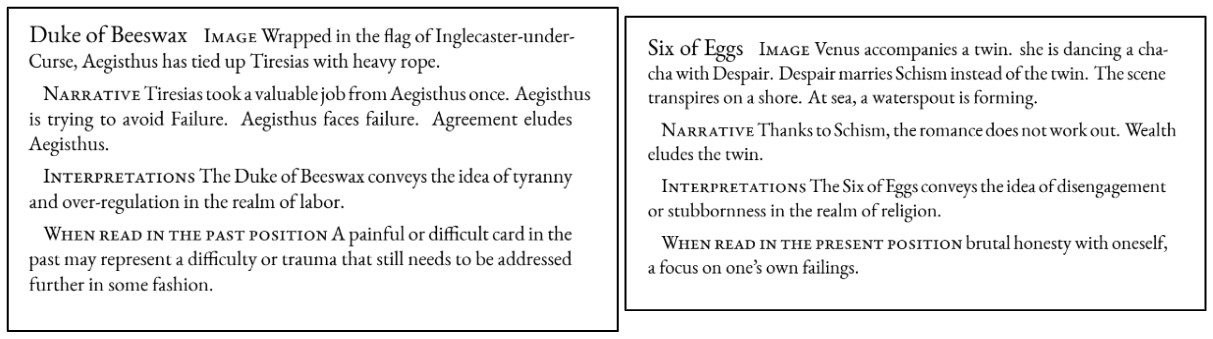
\includegraphics[width=\textwidth]{figures/2-Ice-Bound/parrigues.jpg}
    \caption{Two sample cards from the \textit{Tarot of the Parrigues}.}
    \label{fig:parrigues}
\end{figure}

%%%%%%%%%%%% END FIGURE %%%%%%%%%%%%%%%%%%%%%%%%%%%%%%%%

\textit{Annals of the Parrigues} is a static, non-interactive document, dynamically generated in participation with Kazemi's 2015 ``NaNoGenMo" (National Novel Generation Month) celebration \cite{kazemi_2015}. Short later developed the same system further to create the \textit{Tarot of the Parrigues}, which dynamically generates a Tarot-like deck. The design process iteratively progressed in development through n-gram word association, narrative arc generation, quality control through custom metrics, and custom tagging which allowed for increased narrative causality. The result was cards which contain text descriptions of characters of the \textit{Parrigues}, a brief narrative segment of an event they describe, along with a suggested interpretation (Figure \ref{fig:parrigues}).

These systems again take up the mantle of interlocking thematic constraint, although this time engaging in a sort of meta-combinatorics, generating collections of cards which themselves have a sub-possibility space of potential combinations and expressions.

But beyond generation of cards themselves, we can turn to the more structural, narrative qualities of what kinds of stories systems can enable us to tell. Two main approaches are most relevant to \textit{Ice-Bound}, quality-based narrative systems, and salience-based narrative systems.
%%GDoc comments%% 
\subsubsection{Failbetter and Quality-based Narrative Systems}\label{subsubsec:failbetter-and-qbn-systems}

Failbetter Games is a relatively small indie studio based out of London, known for their flagship game \textit{Fallen London} (first released in 2009) and their more recent games \textit{Sunless Seas} (released in 2015) and \textit{Sunless Skies} (released in 2019). \textit{Ice-Bound}'s development (2013-2016) made it contemporaries with \textit{Fallen London} and Failbetter's StoryNexus engine. 

StoryNexus was the core of \textit{Fallen London}, and was also freely available for people to use to author their own narratives. It had a web-based interface similar to modern Twine, but unlike Twine, possessed an integrated website / marketplace where people could browse and read narratives written with it. This web-based authoring system enabled the creation of what Failbetter calls ``quality-based narratives." These narratives are composed of ``storylets," which Failbetter characterized as ``discrete chunks of narrative that can be played in any order, as many times as you like" \cite{arendt_structuresOne}. These storylets are essentially small pieces of story content bounded by pre-conditions and post-conditions (effects). They each have one or more ``branches" which are the choices made available to the player. Each branch has ``results", which modify qualities. Results can also vary based on success or failure, allowing players to pass or fail ``quality checks." In terms of narrative design, storylets are encountered singly, or in larger interconnected structures called ``Ventures," which are gated and driven by the quality state of the player \cite{ifwiki_2019}.

Qualities are essentially stats. They might be an integer for how many nightmares one has had, a flag for whether a particular storylet has been visited, etc. It's a simple blackboard system, but the design work that goes into Failbetter stories is what makes it really shine, and brings out its complexity.

StoryNexus narratives have some core design assumptions gathered around the metaphor of a card deck. The player has a hand, which can contain a certain number of cards, and an ``Opportunity Deck", which contains a certain number of cards, which can fluctuate wildly in the course of the game depending on the player's qualities, location, or setting (a fact Failbetter narrative designers must anticipate and account for).

Also central to the StoryNexus platform is the concept of ``actions", which are a limited resource, and used every time the player takes an action. They refresh over time, which provides authors a way to meter out and also monetize their content (the two primary ways being ``expansion pack stories" and ``purchase more actions"). It's an interesting platform decision, as it means it is not possible to play through \textit{Fallen London} in one, or even several, playthroughs. This design is ``baked into the content and pacing" such that moving it away from that model would take an estimated 20-25 months of effort on their part \cite{failbetter_ftp}. Some of this presumably is based on the fact that a category of card triggers in StoryNexus games are time-based, but there may be other aesthetic considerations at play as well.

The ability of these stories---told through a series of connected vignettes---to communicate a coherent narrative relies on a design consideration Failbetter calls ``implicit storytelling" or ``fires in the desert." The metaphor is that one imagines the player wandering a dark desert between campfires---we don't need to specify how they got from campfire to campfire. The player can fill in that blank on their own. This design ethos generalizes structurally to the combinatorial nature of the experienced narrative, where storylets may happen in several different potential orders, which doesn't cause problems if the player is given the tools to bridge those gaps on their own. One of Failbetter's founders characterized this approach as making Failbetter games ``a montage: we provide the shots, the player does the arrangement" \cite{arendt_structuresThree}.

\textit{Fallen London} is an immensely successful combinatorial narrative. It is also a very large combinatorial narrative. Conservatively, there are more than 2000 root-level storylets \cite{fallen_london_wiki}, not counting the associated content for each of a player's available choice options and outcomes for each one (which their authoring guide broadly suggests should number around five per storylet). The total word count is in the neighborhood of 1.5 million words \cite{failbetter_ftp}, spread between a team of several authors. This sort of undertaking demands rigorous systemic design knowledge and practices in order to make authoring tenable.

Due in part also to StoryNexus being a platform and public community of practice, Failbetter was motivated to formalize and make public several authoring patterns and design practices they used in crafting their combinatorial narratives. There are more than 60 different authoring patterns, split between content design \cite{storyChoices_contentDesign}, branch design \cite{storychoices_branchDesign}, and choice design \cite{storyChoices_choiceDesign} (although these distinctions overlap and can be somewhat muddy). Some examples can be seen in Figure \ref{fig:storynexus-patterns}.


%%%%%%%% BEGIN FIGURE %%%%%%%%%%%%%%%%%%%%%%%%%%%%%%%%%

\begin{figure}
    \centering
    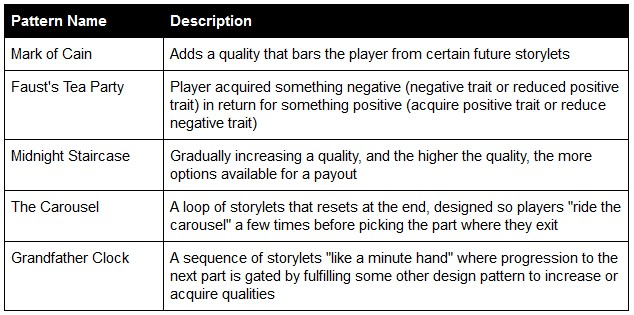
\includegraphics[width=\textwidth]{figures/2-Ice-Bound/storynexus-patterns.jpg}
    \caption{A selection of StoryNexus authoring patterns.}
    \label{fig:storynexus-patterns}
\end{figure}

%%%%%%%%%%%% END FIGURE %%%%%%%%%%%%%%%%%%%%%%%%%%%%%%%%

These authoring patterns were intended to be used in specific, grounded cases, but there is also some generalized design advice for authoring with StoryNexus. Most salient to our pursuit of practices increasing authorial leverage is Failbetter's notion of ``quality parsimony."

Quality parsimony means reducing the number of unique entries into the state blackboard (qualities) as much as possible during the design/authoring process. This simple rule has some long-reaching structural effects. Failbetter opted for this type of narrative design instead of a more traditional branching pattern, wanting their stories to structurally resemble more ``a river rather than a tree [...] You want any one character [here meaning the player] to see 90\% of your content, not 50\% or 10\%" \cite{arendt_structuresThree}. One could see this mapping to the Authorial Leverage framework as wanting to increase authorial Clarity, such that---as the number of storylets grows---there isn't a concomitant growth of the blackboard state such that it  becomes untenable for authors to easily hold it in their mind as they plan and write future Ventures.

The hours poured into design resources and documentation of StoryNexus enabled a rich and varied community, with large and elaborate combinatorial narratives that afforded writers with little programming background the ability to create procedural stories, and even monetize their efforts. This lead to amazingly complex and baroque works (quality parsimony aside) such as \textit{Black Crown} by Rob Sherman, which engaged with the unique limitations of the StoryNexus platform (such as the limit to player actions) as diegetic material arising from its fictional world \cite{reed_blackCrown}.

StoryNexus as a platform, unfortunately, did not prove to be sustainable over a long period of time. Even with support from Random House, projects like \textit{Black Crown}---with their concomitant ``unique features and separate, demanding bug queue" \cite{sherman_2014}---proved too unwieldy, and the labor required to support them untenable. StoryNexus was officially shuttered near the end of 2013 due to the monetization of the platform being insufficient to support platform maintenance and development. Failbetter had just successfully run a Kickstarter for their new property \textit{Sunless Sea}, and decided to consolidate their efforts around developing and launching that game in the new modality, leaving StoryNexus as an archival body of community-authored work in testament to the early system \cite{kennedy_2013}.

\paragraph{Similarities and Differences.}\label{par:storynexus-similarities-and-differences}

While the combinatorial nature of StoryNexus's system was definitely something similar to what we wanted in terms of \textit{Ice-Bound}'s dynamics, a big difference was that we wanted the experience of an \textit{Ice-Bound} level to be more about exploring a narrative possibility space through quickly making easily-reversible choices. The feeling we were trying to capture was more an editorial one, or as Reed put it, a ``sculptural" one. This meant that, unlike StoryNexus games which hinge around the idea of progress through a series of choices that can occur in different orders, but which permanently affect the state space, we wanted a game where many ``choices" could be made and reversed, until the player had a path through the story they were satisfied with. While the systems under the hood might have some similarities, it is this key difference that distinguishes the \textit{Ice-Bound} system and approach from StoryNexus games. Additionally, we wanted players to be able to make as many changes as they wanted, unmetered and unlimited, as opposed to StoryNexus's approach with their actions.
%%GDoc comments%%
\subsubsection{Salience-Based Narrative}\label{subsubsec:salience-based-narrative}

This sort of experience architecture, where content is selected based on underlying qualities driven by player interaction, has a close cousin. If we consider instead that the system is evaluating player input and state, in order to \textit{automatically} select the most salient content to display, we can use the lens of what Short calls ``salience-based narrative" \cite{short_salience}. The heuristics driving content selection can be very simple, yet create compelling experiences when supported by proper design.

A good example of this can be seen in Barlow's \textit{Her Story} \cite{barlowe_her_story} and \textit{Telling Lies} \cite{barlowe_telling_lies}, two narrative games whose only interaction is through entering database queries to different short film segments. In \textit{Her Story} these are recordings from a police office as they interview suspects for a murder. In \textit{Telling Lies}, the videos are one-way recordings of characters' webcam input, forcing the player to try to piece together the story's dialogues across clips.

For both, the player's interaction is restricted to entering text queries into a diegetic search engine. The game then goes through the library of content, and presents video clips that match (Figure \ref{fig:barlow}). While this is deceptively simple, the finesse of the experience is wholly in the design of the interface and the manner in which the videos are tagged. For example, in both experiences only five video results will be displayed, even for terms which have more than five results. Thus, the reader's strategy of finding content evolves very quickly from queries like ``murder" to more specific ones referencing information they've gleaned from more general clips. Also, the tagging itself is a mixture of thematic and keyword-driven excerpts from the clip transcripts.

%%%%%%%% BEGIN FIGURE %%%%%%%%%%%%%%%%%%%%%%%%%%%%%%%%%

\begin{figure}
    \centering
    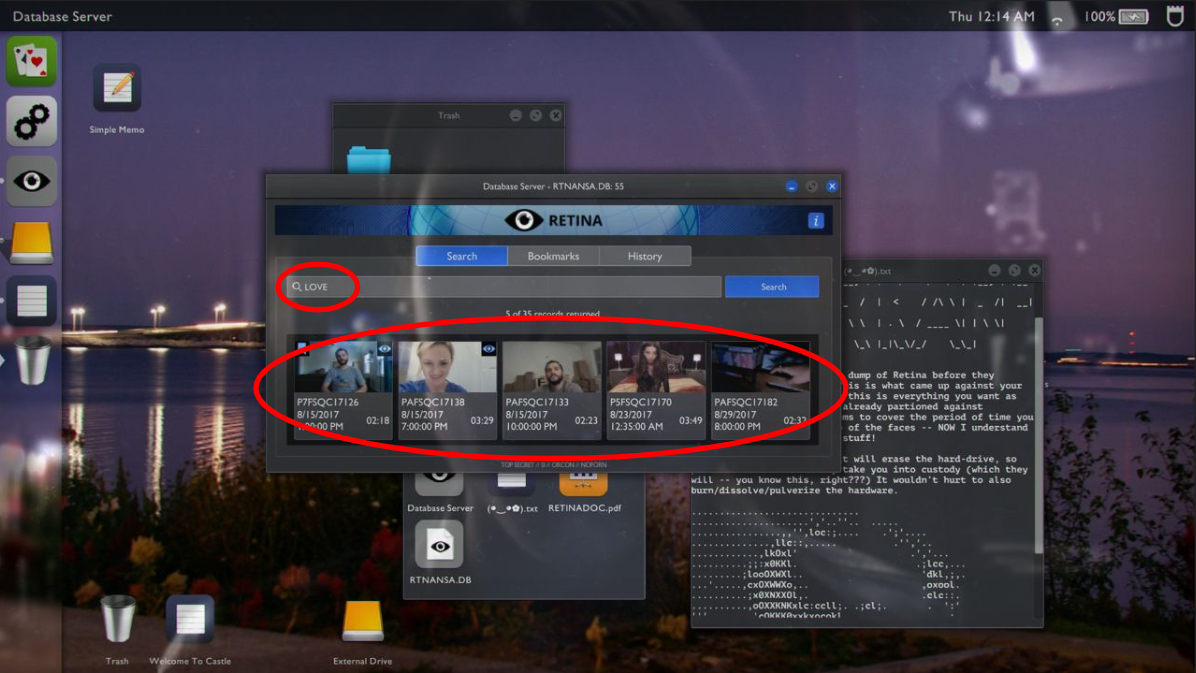
\includegraphics[width=\textwidth]{figures/2-Ice-Bound/barlow.png}
    \caption{A screenshot from Telling Lies, with the search term ``LOVE" circled, and the resulting five video clips that match that term circled.}
    \label{fig:barlow}
\end{figure}

%%%%%%%%%%%% END FIGURE %%%%%%%%%%%%%%%%%%%%%%%%%%%%%%%%

Barlow has skillfully designed a database such that, because one can only know terms after watching certain clips (such as the importance of the suspect's guitar in \textit{Her Story}) the available exploration pattern---discounting pure luck---could be viewed as a choice-driven tree structure, where each ``choice" is one of the clips brought up in the query.

Of course, more complex tagging examples exist. The prevalence of tag- and trigger-driven content has been around in first-person style games for quite some time. One more recent example that is especially colorful is the indie game \textit{Firewatch}. In it, the player takes on the role of Henry, a ranger who's been assigned to a fire watchtower for the summer. The bulk of the game's content comes from communication through a handheld walkie-talkie and radio with Delilah, a fellow ranger stationed in the neighboring tower.

What makes this interesting is that the conversations for \textit{Firewatch} are all contextually triggered by actions the player takes in the game. As noted in a Slate interview with Vanaman, Firewatch's main writer:

\begin{quote}
"The conversation is putting itself together dynamically, and that means it can be hyper-specific,” said Vanaman. “There are 10,000 events in the game—speech and everything else—that can happen.” Rather than simply shunting you from branch to branch of a dialogue tree, the game looks at everything you’ve said and done, and picks the truest and most specific thing that can happen next. “There are so many [variables] in our game that are so silly and weird. There’s stuff like, has Henry ever mentioned the outhouse? Maybe that matters." \cite{hudson_2016}    
\end{quote}

\paragraph{Similarities and Differences.}\label{par:salience-similarities-and-differences}
In a way, the pre-condition logic \textit{Ice-Bound} uses for determining what content to show bears similarity to the design methodology for salience-based narratives. On a code and general software architecture level, we're reacting to player actions, and determining the ``most salient" content to display. However, from a design perspective, the pre-condition logic is much more geared around narrative coherence with what the player has chosen to make active in the story, as opposed to reactive to diegetic actions the player may take in a story world. And while the use of continuous thematic context (discussed in Section \ref{subsubsec:25-themes-and-12-tags}) allows for a similar experience to Barlowe's use of progressively specific keyword tagging, we leverage that in a more systemic way for \textit{Ice-Bound}'s finale (discussed in Section \ref{subsubsec:thematic-finale}).
%%GDoc comments%%
\subsubsection{\textit{King of Dragon Pass} and \textit{Six Ages}}\label{subsubsec:king-of-dragon-pass}

Another game in dialog with \textit{Ice-Bound} is David Dunham's \textit{King of Dragon Pass}, first released in 1999, but ported twelve years later in 2011 to iOS. Dunham himself provided a nicely succinct description of his game \cite{dunham_2011}, saying it

\begin{quote}
essentially has an underlying resource management game which serves as the skeleton that supports the stories. [...] Play consists of alternating resource-related actions, and responding to story scenes. These consist of an illustrated situation, usually with five choices. These may lead to secondary choices, but still within the same situation, until it’s resolved. Resolution may have specific later consequences, but typically influences the economic model of the resource management game. Parts of the story and setting are actually revealed through your advisors, individuals you pick to sit on the clan council. While you can lose the game through poor resource management (or bad luck), you can only win by story choices.    
\end{quote}

In contrast to StoryNexus games, \textit{King of Dragon Pass} and \textit{Six Ages} both obscure the ``qualities" driving the logic of different scenes, a decision Dunham said was made out of a desire to prevent the presence of statistics from ``breaking the fantasy" of the world. Additionally, he admitted to randomness playing a larger part as well, compared to the more deterministic combinatorial paths through the multitudinous decks of StoryNexus works.

\textit{King of Dragon Pass} conforms as well to the same ``choice metric" Failbetter suggests, with five choices per ``scene" if possible. Dunham keeps runaway content contained by limiting these scenes to one or two choices, after which the stats are adjusted, and play continues in the simulation. This sort of modular design keeps the chances of unforseen long-term combinations or effects from sabotaging gameplay. 

\textit{King of Dragon Pass} sports 500 events, which makes the pool smaller than Failbetter's games, though it is still more than enough to incur substantial authorial burden, especially when taken into consideration with the potential knock-on effects from the simulation system running alongside it, including both an economy and a social model. Additionally, the simulation allows different ``modes" of player actions---such as sending a caravan or setting ratios of crafting quality---which have a more systemic effect than the more atomic actions players take in StoryNexus games \cite{dunham_repeatability}. While events may repeat, it will typically be a substantial period of time before they do, and Dunham relies on the context of the event's recurrence changing the encounter enough that it retains its interest.

This event dynamism comes by virtue of the DSL (domain specific language) Dunham created for \textit{King of Dragon Pass}, and later elaborated upon for \textit{Six Ages}. OSL (Opal Scripting Language) is meant to be more approachable for the writer than coding in C++, the language both were originally written in. OSL affords dynamic character casting, so that recurring events can star the same characters, or characters can be cast by trait. It also allows randomized or trait-dependent text display, which---when paired with pre-condition logic checks for traits---keeps events salient to your decisions as the game progresses \cite{dunham_2008}.

\paragraph{Similarities and Differences.}\label{par:dragon-pass-similarities-and-differencs}
\textit{Ice-Bound} shares storytelling approaches with the system in \textit{King of Dragon Pass}---we similarly wanted to have self-contained vignettes gated by pre-conditions, and use a simple blackboard structure to drive that. However, as with our difference from StoryNexus, we wanted to pursue a mode of interaction that was more about continuous editing and undoing of changes, to give a more exploratory feel. \textit{Ice-Bound} also makes use of character casting for its components, which adds to the dynamism of scenes. Also, we had no desire to impart any kind of simulation to the game, which \textit{King of Dragon Pass} uses in concert with its narrative to drive the experience. The ``window into procedurality" we wanted to provide was rather through exposing the conditions themselves, so that---unlike Dunham's position that knowing underlying state variables breaks the fiction---players know exactly the reason content displays, and can use that to further enrich their strategies for exploration.


\section{Relationship to Related Works}\label{sec:ice-bound-relationship-to-related-works}

Situated in dialogue with this body of combinatorial narrative, \textit{Ice-Bound}'s development was uniquely positioned to offer an experience geared around enabling the reader to make low-friction, frequent changes to a narrative possibility space, coupled with vignettes of a substantial length with high quality surface text, yet still causally connected via their pre-condition logic. The incorporation of conversations with a character using more traditional branching choice structures injected a note of familiarity, and the incorporation of material into a printed book provided a more ``static traditional medium" to convey longer pieces of the story.

\section{System Description}\label{sec:ice-bound-system-description}

\subsection{Summary}\label{subsec:ice-bound-summary}

\textit{Ice-Bound} consists of three systems, two of which operate primarily as a support for the central one. The central system is a combinatorial narrative system (Figure \ref{fig:ice-bound-system}), which drives the main narrative. This is supported by a tag-based content selection system (used when scanning pages from the book) and a branching dialogue system (used for dialogues with the character KRIS).

%%%%%%%% BEGIN FIGURE %%%%%%%%%%%%%%%%%%%%%%%%%%%%%%%%%

\begin{figure}
    \centering
    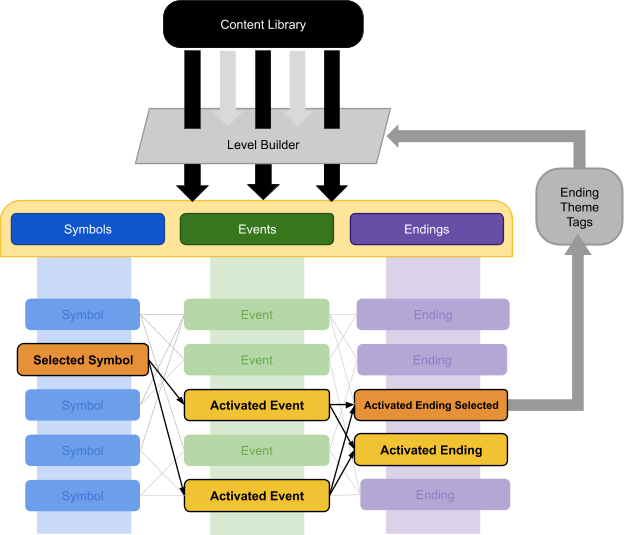
\includegraphics[width=\textwidth]{figures/2-Ice-Bound/ice-bound-system-diagram.png}
    \caption{A diagram of the flow in the combinatorial narrative system. Content is filtered and selected through the Level Builder. Valid symbols, events, and endings are displayed. The player then selects whatever symbols they desire, which in turn activate events, which in turn activate endings. When the reader is satisfied with a given set of activated symbols, events, and an ending, they select the ending. The thematic tags of that ending are then added to the filter logic of the Level Builder, the next level's content is selected, and the cycle begins again.}
    \label{fig:ice-bound-system}
\end{figure}

%%%%%%%%%%%% END FIGURE %%%%%%%%%%%%%%%%%%%%%%%%%%%%%%%%

\subsubsection{Combinatorial Narrative System}\label{subsubsec:combinatorial-narrative-system}

The main \textit{Ice-Bound} game interface is ``blueprint mode" (Figure \ref{fig:blueprint}), which shows a blueprint-style overview of the current level's rooms. Each room has some number of sockets (the ``cigar box" or ``round table" in Figure \ref{fig:blueprint}), each of which is tied to a particular symbol card. Each level, the player is provided some amount of ``light", symbolized by glowing yellow circles, that they can drag around onto sockets to activate the symbol cards.

There are three types of cards in the system: symbols, events, and endings. The player can directly activate or deactivate symbols by moving the light. Combinations of activated symbols in turn activate or deactivate events, and combinations of activated symbols and events in turn activate endings.

%%%%%%%% BEGIN FIGURE %%%%%%%%%%%%%%%%%%%%%%%%%%%%%%%%%

\begin{figure}
    \centering
    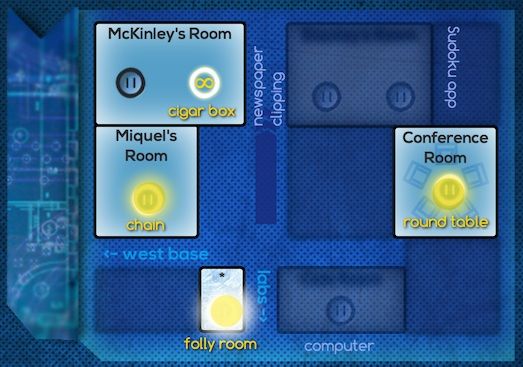
\includegraphics[width=10cm]{figures/2-Ice-Bound/blueprint.jpg}
    \caption{The blueprint UI of an \textit{Ice-Bound} level, showing sockets in rooms. Here we see ``chain", ``folly room" and ``round table" are activated, ``cigar box" is always activated, and ``computer" etc are not activated.}
    \label{fig:blueprint}
\end{figure}

%%%%%%%%%%%% END FIGURE %%%%%%%%%%%%%%%%%%%%%%%%%%%%%%%%

These linkages are established through an authoring convention of content tagging, and simple propositional logic. Most event and ending conditions are based on whether certain symbols or events are active, or symbols and events with particular tags are active. More specific system details will be elaborated on in Section \ref{subsubsec:icebound-complexity}'s discussion of Complexity.

\subsubsection{Tag-based Content Selection System}\label{subsubsec:tag-based-content-selection-system}

When a player has activated symbols such that the resulting story is one they are happy with, they're asked by KRIS to ``confirm he would write something like this" by scanning a page from the book that matches the ending's theme.

\textit{Ice-Bound} uses marker-based augmented reality tracking, so that when the scan mode is activated, players can point the camera of their iPad or computer at the book, and images will display on the pages, revealing further narrative details, or providing some piece of context for how they fit into KRIS's life. The book's format provided us with a chance to write longer story sections, which stood in contrast to the more generative, vignette-like narrative of the digital game. 

Each page in the \textit{Ice-Bound Compendium} is tagged with some number of thematic tags. In contrast to the symbols, events, and endings, these tags are invisible to the reader, prompting a sort of ``thematic scavenger hunt" to find a page which fits the ending selected by the reader. These hidden tags for each page drive recurrent threads or themes throughout the book, but there isn't a set or canonical order to the pages. One might follow the thread of Kris's relationship with his daughter by finding pages scattered throughout detailing its deterioration across multiple themes, but the arrangement of pages was more to provide an equal distribution of tags than any sort of chronology. This was done in order to encourage players to flip through it at length, and reinforced the ``editorial" mode of searching in a body of content for specific evidence to fit a particular narrative.

\subsubsection{Branching Dialogue System}\label{subsubsec:branching-dialogue-system}

%%%%%%%% BEGIN FIGURE %%%%%%%%%%%%%%%%%%%%%%%%%%%%%%%%%

\begin{figure}
    \centering
    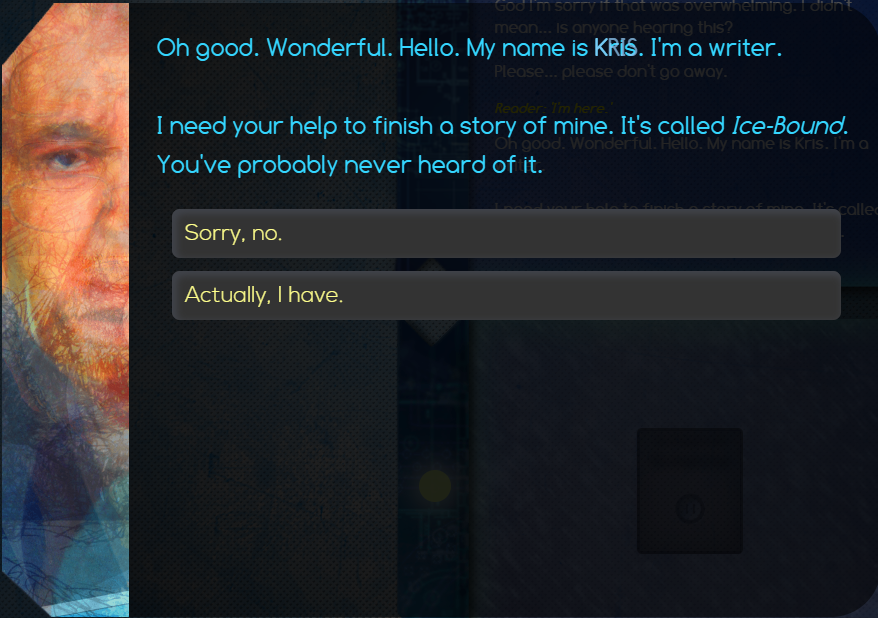
\includegraphics[width=10cm]{figures/2-Ice-Bound/kris-dialogue.png}
    \caption{A screenshot of the dialog system in \textit{Ice-Bound}, where the reader would experience traditional choice-based narrative segments.}
    \label{fig:kris}
\end{figure}

%%%%%%%%%%%% END FIGURE %%%%%%%%%%%%%%%%%%%%%%%%%%%%%%%%


Part of \textit{Ice-Bound} is also talking with KRIS via pop-up branching dialogues. These are done in the usual manner of branching dialogue, where content is authored with links to other content, and the responses the player clicks are their replies to the content displayed. These dialogues have their own state-driven conditions and effects, which allowed us to author dialogues that only appear if symbols with certain tags are activated, or a specific symbol is activated. Combined with state-sensitive templating, this means we could write dialogues with KRIS that leverage the current context of the narrative the player is crafting with great specificity, while still advancing a fairly linear narrative of KRIS's background, and how he was created. The experience this enables is one where KRIS feels like a collaborator who is sensitive to the changes you are making to the story, and that particular context sensitivity is a critical part of communicating that the system is "listening" to the choices the player is making, and that those choices have meaning.

\subsubsection{State-driven Templating and Shimmertext}\label{subsubsec:state-driven-templating-and-shimmertext}

%%%%%%%% BEGIN FIGURE %%%%%%%%%%%%%%%%%%%%%%%%%%%%%%%%%

\begin{figure}
    \centering
    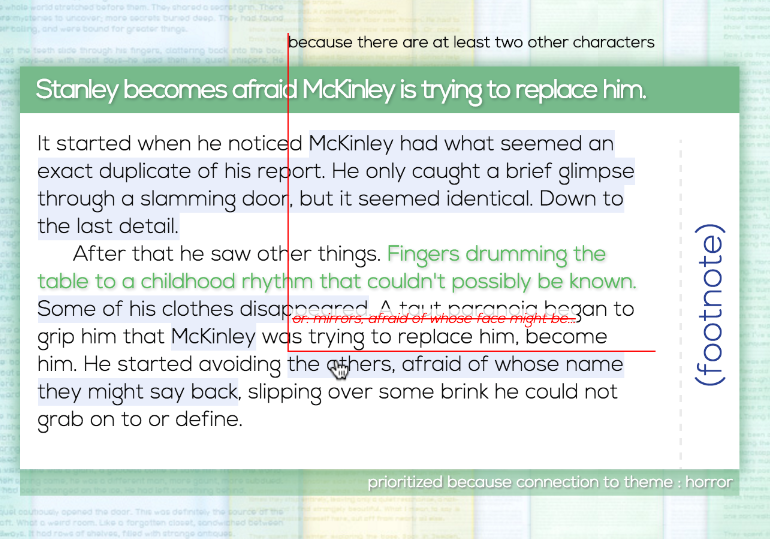
\includegraphics[width=\textwidth]{figures/2-Ice-Bound/event.png}
    \caption{An event in the longer-form portrait-view interface. Note the dynamic text (``McKinley had what seemed an exact…") the shimmertext (``Fingers drumming the table…"), the tooltip-style explanations (``because there are at least two other characters") and the theme trigger text in the bottom right (``prioritized because connection to theme: horror"). The ``footnote", when clicked, starts a KRIS dialogue.}
    \label{fig:event}
\end{figure}

%%%%%%%%%%%% END FIGURE %%%%%%%%%%%%%%%%%%%%%%%%%%%%%%%%


All three systems make use of state-driven templating to change their surface text---sometimes substantially---in order to increase relational cohesion through the different pieces of content displayed to the reader. These were used to keep character casting coherent between fragments, so that the protagonist and antagonist in one fragment would be the same in the next, as well as to bring in key pieces to reinforce flavor from an earlier fragment.

We also made heavy use of ``shimmertext", which is text that shifts between different options continuously. This text styling is supposed to represent places of the story KRIS isn't ``sure about", and the player can help resolve them by tapping on them. Tapping once solidifies the text so it stops shifting, and subsequent tapping cycles the text between its different options. This was a handy catch-all for situations where we wanted to write state-dependent or ``sensible" variation for text, but didn't want to commit to tracking it in the blackboard state or bogging down the pre-conditions. We would simply write the options as ``shimmertext", and rely on the reader to exercise their editorial control to resolve them ``sensibly." Or not! Some players enjoyed the spice of mystery injected into a scene if a character suddenly grimaced at happy news, or seemed happy at misfortune. The fictive framing for this was that it was a shortcoming of KRIS as an artificial entity if they didn't match up, a framing we intentionally leaned into so that, even if the system fell short, it was still a diegetic failure, and not a fiction-breaking one.

\subsubsection{Why the System Works}\label{subsubsec:why-the-system-works}

From a storytelling perspective, \textit{Ice-Bound} makes use of a few ``tricks" to get around some of the pernicious problems with story generation.

As mentioned earlier, we leveraged StoryNexus's design concept of implicit storytelling or ``fires in the desert" \cite{arendt_structuresThree}. As storytellers, we don't need to concern ourselves with what happens between the campfires. The reader can fill in those details, or imagine logically what happens for the character to move between the fires. Scott McCloud had a similar concept called ``blood in the gutter" \cite{mccloud_1994} to refer to action that happens between the panels in the comic. These are narratological leaps the reader is willing to make, ones which, if elided, don't cause too big a disjunct in the reader's model of the story, and can be safely left unspoken. Another way to formulate this is Murray's concept of narrative ``anticipation" and ``dramatic compression." Simply put: as long as the fragments we show the reader shore up and advance the characters or play into narrative conventions, the reader can abstract the rest of the scaffolding necessary to make them sensible \cite{murray_compression}.

Our initial prototype had the player moving between rooms, moving objects, and in general had a more simulationist bent. What we found, though, was that the demands of simulation were moving us further and further away from what we had started out in the project to do: tell a complex, compelling story. After bumping up against simulation complexity when proposing a new part of the story, we decided to shift the design away from that, and let the reader connect the dots themselves. We also didn't want to focus too much on what was ``logical" and therefore ``allowed" in the story, if that meant stifling the player's agency.

The templating system therefore, provided just enough dynamism to keep the campfires in sight, so to speak. Our fictional framing---that the story was riddled with errors and bad drafts---also helped ``frame the failure" such that when our system fell down, we could rely on the player to move away from those mistakes, and even to see them as aesthetic choices we had made \cite{reed2014ice}. As noted earlier, this cohesion bolstering was also accomplished by using shimmertext when we weren't sure or didn't have time to model dependencies for certain sentences or words within sentences. The important thing is that the core causality for these events was preserved as they flowed to create a story for the chapter.

In the course of writing and testing, we found anecdotally that mismatches between time and location were fine, because players would assume a subsequent scene took place later, or was a flashback. More problematic would be when player qualities or emotions didn't seem to match up, where a character's reaction to one event when it happened was anger, but in a later event referencing it, the character was said to have been happy. This led us in writing the cards to craft pieces of story that were relatively self-contained, but had a few tendrils here and there reaching out, usually in the context of their theme or themes.

\subsubsection{25 Themes and 12 Tags}\label{subsubsec:25-themes-and-12-tags}

\textit{Ice-Bound}'s narrative design also makes use of tagging in various ways to provide consistency, and heighten the sense of responsiveness in the system over time.

%%%%%%%% BEGIN FIGURE %%%%%%%%%%%%%%%%%%%%%%%%%%%%%%%%%

\begin{figure}
    \centering
    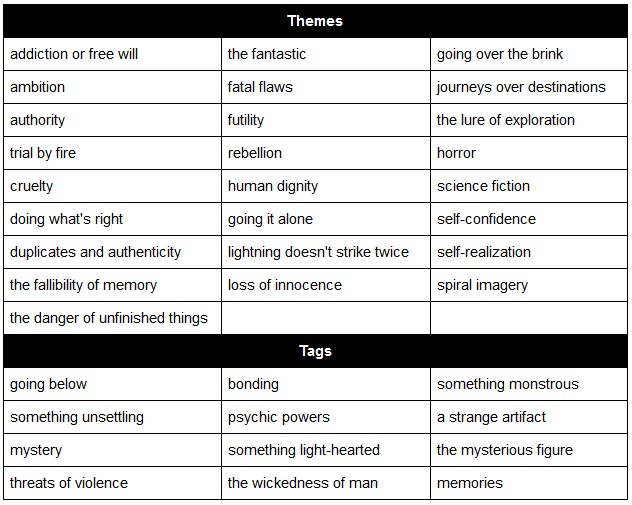
\includegraphics[width=\textwidth]{figures/2-Ice-Bound/themes-and-tags.jpg}
    \caption{Themes and tags used in \textit{Ice-Bound}.}
    \label{fig:themes-and-tags}
\end{figure}

%%%%%%%%%%%% END FIGURE %%%%%%%%%%%%%%%%%%%%%%%%%%%%%%%%

In the course of creating the story, we categorized content broadly into 25 themes. Each piece of content, whether it was a symbol, event, or ending, could have two or three themes applied to it. This was used mainly for the triggering logic between them, so that we could target broad categories of content when necessary. However, it also had another use.

When the player confirms an ending that they think is best, find it in the book, and scan it in using AR, KRIS has a dialogue with them about the page. Each page has roughly three to five themes, and he asks the player which one of them they were thinking of primarily. When the player makes their suggestion, KRIS then picks another theme on the page as one he ``likes" as well.

When the next level is generated, the symbols selected to populate it take into account the themes the player has selected. This means that, as the player continues in \textit{Ice-Bound}, they can end up with stories that cleave closer to the type of content they want to see. Sometimes these differences can be quite noticeable, in the case of more obvious themes like ``science fiction" or ``horror."

\subsubsection{Thematic Finale}\label{subsubsec:thematic-finale}

We wanted to do something special for the finale of \textit{Ice-Bound}, something that would show that all the choices the player had been making along the way had been building towards something. More than anything, we wanted to avoid a situation where the player felt that the ending was ``pre-baked" and only had slight differences depending on their choices. However, we also didn't want to commit to something that would put undue burden on us, such as a wholly new system or mechanic. And we didn't want to commit to a lot of custom authoring, which would most likely never be seen by most players, given the relatively low completion rate of \textit{Ice-Bound} playthroughs as a whole.

%%%%%%%% BEGIN FIGURE %%%%%%%%%%%%%%%%%%%%%%%%%%%%%%%%%

\begin{figure}
    \centering
    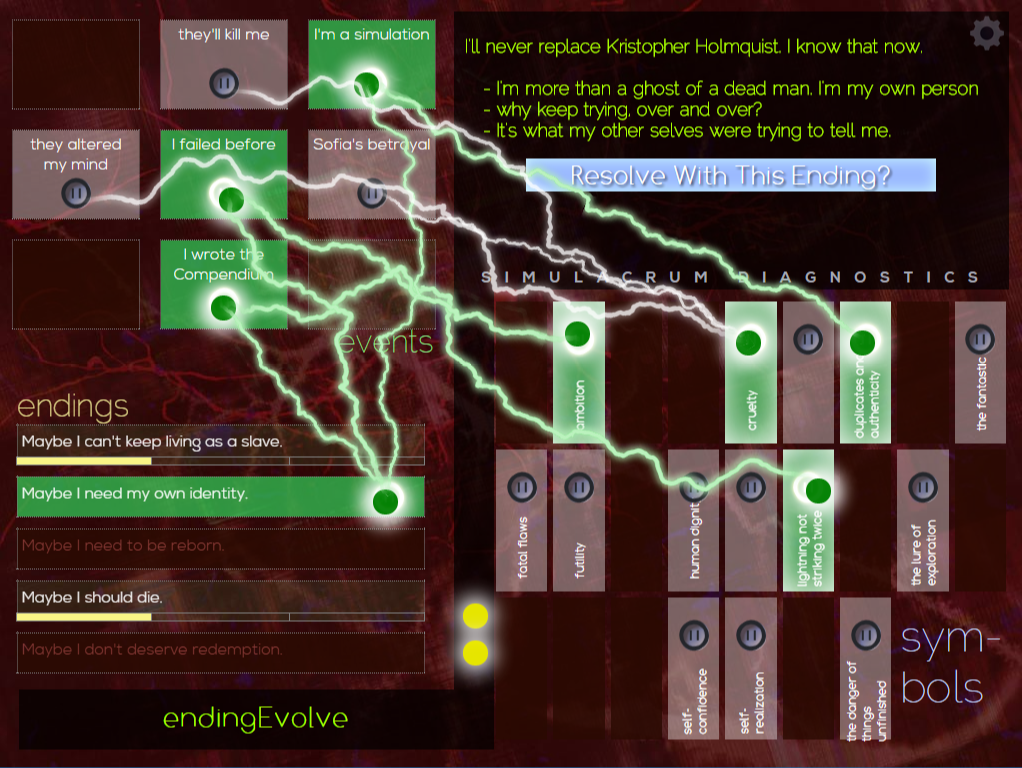
\includegraphics[width=\textwidth]{figures/2-Ice-Bound/finale.png}
    \caption{The final level. The player still drags lights onto symbols (which are now themes) which activate ``events" (KRIS's self-realizations) whose text is in the upper left (``why keep trying, over and over?") and when all three required events are activated, the ending lights up (``Maybe I need my own identity").}
    \label{fig:finale}
\end{figure}

%%%%%%%%%%%% END FIGURE %%%%%%%%%%%%%%%%%%%%%%%%%%%%%%%%

Our solution was to use the themes players (and KRIS) activated in the course of their playthrough as the ``symbols" for the final level. The story of this level is the story of KRIS's life---the justification for the ending action he will take, which can range from escape to self-destruction. In a manner now familiar to players, they drag the lights to activate the themes, which ``electrify" to activate the ``events." In this case the events are more ``justifications" for the action KRIS will take, drawn from information the player uncovered through the course of play, and re-contextualized as justifying a particular action (in Figure \ref{fig:finale} it's ``I'll never replace Kristopher Holmquist”). When all three associated justifications for an action are activated, the ending is unlocked. In Figure \ref{fig:finale} we can see it is ``Maybe I need my own identity."

Because the combinatorics of this play into the same content production flow as earlier levels, there was very little extra code needed to produce this finale. And because the materials are drawn from the symbols and secrets the player has uncovered through their play, it feels customized and unique. Selecting the ending action plays out one of five final custom branching dialogues with KRIS, which also makes use of templating to change the surface text details to match the particular combination used to activate it.

\section{The Question of Authorial Leverage}\label{sec:the-question-of-authorial-leverage}

\subsection{Traversability}\label{subsec:icebound-traversability}
In order to understand the tool support and design decisions made to tackle the authoring task the experience required, we need to first understand the quality of the space fulfilled by the system. This is the question of Traversability, which breaks down into three sub-questions: Explorability (how much content the player can see per playthrough), Replayability (how much of the content is seen by the player in one playthrough, and how many playthroughs is the player expected to undertake) and Reusability (how often content can be reused).

We will tackle each of these in turn. Having done that, we will be well-positioned to detail the different strategies to address the space they describe, in the following section on Authorability.



\subsubsection{Explorability}\label{subsubsec:icebound-explorability}

One of \textit{Ice-Bound}'s strengths lies in the broadly explorable space it provides its players. This was necessary to provide a player experience as one of ``sculptural fiction" (making many low-risk, reversible choices). This is accomplished through a high degree of variability: each socket in a level can be potentially cast with different symbols (although the pool of valid symbols to draw on differs case-to-case). For example, in the third level in the game---about mid-way through the experience---there are technically around 50,000 different combinations of symbols that can be activated, depending on which themes have been strengthened in the previous levels.

That's a large number! But in terms of \textit{meaningfully different} combinatorics, the sets of activated content that feel qualitatively different is smaller, especially given events are typically triggered by tags or themes, which are much more coarsely-grained groups. As mentioned earlier, there are 37 themes/tags content can be tagged with. However, a piece of content can have many tags, thus flexibly collapsing the combinatorics given the discretion of the author. For example, if we authored three pieces of content each tagged with twelve themes, effectively we’re only dealing with combinatorics of three “groups” of tags.  The number of tags per-content piece fluctuates greatly, but in general we would have around three to five themes per symbol. This still means a very broad array of possible content can present itself, especially given that an activated symbol could not only trigger new events (and thus new stories) but also impart qualities to characters, who may be in multiple pieces of content. For example, activating a symbol like ``borrowedKnife" flags the character Miquel with ``guilty", which can change the text that appears in a later event, even if the event itself is not novel.

We knew from a pacing standpoint that we wanted to create eight levels, in order to give us space to tell eight generative stories, and give the player time to become familiar with the system, as well as the many layers of permutation it affords. We also determined that on average, given the number of sockets we wanted to give the player to activate, we wanted to provide about three ``global" sockets per level, in order to provide a way for player-selected themes from previous levels to express themselves. Given that each ending had three to five themes, some rough math meant that if we had about three global symbols per theme (about 75 in total) it would be enough that we could respond to player theme selection.

How much of the total content is explored by the player by the time they have completed a playthrough depends widely on their play style. \textit{Ice-Bound}'s mechanic for revisiting earlier levels means that technically players could see 100\% of the story content, although the exhaustive nature of that makes it very unlikely. Anecdotally across playtests and once the game was released, we saw that players tended to fall into two broad groups: some would go very deep on a particular set of symbols they wanted to engage with. They would take the time to explore their combinations, reading the full text of the events and endings they activated in the ``portrait view", and customizing the shimmer text. Others would go very wide, spending most of their time in the ``blueprint view" and changing symbol activations, and more exhaustively explore the combinations themselves. But, once they switched to portrait view to read the story they'd created, they seldom made further changes.

It would be an interesting and worthwhile pursuit to build a tool to simulate playthroughs and measure the percentage of total content that is ``activated" by a given playthrough, to provide a sense of how much content is being used or re-used. One could imagine it as an addition to \textit{Ice-Bound}'s existing authoring tools detailed in Section \ref{par:icebound-combination-browser}, which make use of automated playthroughs to collate data on the state of the content library. However, we found--having set up particular constraints in the prototyping phase and roughing in content---that the level of explorability we were shooting for was sufficiently high, while still being achievable from an authoring standpoint, so no further support was needed in this area.

\subsubsection{Replayability}\label{subsubsec:icebound-replayability}

Because of the aforementioned dynamism that's driven by player-chosen themes as they progress, \textit{Ice-Bound} is highly replayable as an experience. As designed, we hoped that players really engaging with the work would adopt one of two strategies: perusing through many permutations of each level, and then settling on one combination that they particularly enjoyed, or replaying the game from the beginning quickly, exploring how their choices echoed through the game's different levels and stories as it progressed. This design goal meant that we needed enough content to not feel ``same-y", and to give enough control over variation that the player would feel like a co-author alongside the troubled AI KRIS. Additionally, while KRIS dialogues were the traditional choice structure, their triggers were driven by the activation state of the symbols, and thus (in a way) ``combinatorially revealed." It was therefore easy for repeated playthroughs of the game to trigger different ``static" conversations with the player's collaborator, which helps increase the replayability. In general, however, we planned mostly for one playthrough, though one whose changeful affordances meant that subsequent playthroughs could be easily accommodated.

\subsubsection{Reusability}\label{subsubsec:icebound-reusability}

Content in \textit{Ice-Bound} had a varied amount of reusability. Some content was restricted to a single level (or even a single socket!) whereas the global symbol cards could show up at any point of the game. Similarly, there were KRIS dialogues with a range of applicability. The \textit{Compendium}, of course, was always present, and thus afforded a ubiquitous availability of content and theme throughout a player's experience.

The global cards in particular were the focus of our efforts in reusability. Having a global card with certain themes could provide critical fallback coverage if we couldn't ensure that level-specific content would be appropriate for the player's context. These were more difficult to write at times, because we also wanted the text to be contextual to wherever it was used, and thus had to make much heavier use of state-driven templating. Additionally, their precondition logic needed to be more complex, which in turn required more checking to make sure they worked in all their contexts.

At the end of a level, the player selects a page from the \textit{Compendium} that supports the ending they chose for the level's story. Then, the game prompts them to choose which theme from the page they wish to ``strengthen." Once we do that, we deploy a clever trick to maximize content reusability. KRIS, in the spirit of collaboration, selects a theme as well. This is a design trick purely in service of reining in combinatorial explosion. The system looks at the currently valid content for the next level given the player's chosen themes, and then picks a currently-unstrengthened theme that puts as much content as possible into play. This was used to combat the implication that, by the end of the game, we conceivably would run into ``meta-combinatorics" of needing to have enough content written for someone hammering home on one particular theme every level. Ensuring a mix of themes meant we could lower the authoring requirements significantly.

Core also to making content reusable was the state-driven templates, which could make use of dynamic casting, character qualities, and what other symbols were currently activated to shape their text into something that could tie in with a story told in a multitude of settings.

In a given playthrough, cards were seldom reused between levels. However, across many playthroughs, or taking all playthroughs of \textit{Ice-Bound} as a data point, there is a very high amount of reusability. The same card may show up in dramatically different contexts, and---with the assistance of the state-driven templates---mean very different things to the player's story. Therefore, content was ``reusable" in the sense that one piece could occupy multiple locations within the content library, which is definitionally at the heart of combinatorial narrative.

\subsubsection{Contextuality}\label{subsubsec:icebound-contextuality}

Content that reacted and reflected player choices and game state was very important to \textit{Ice-Bound}. The player choosing themes that sculpt the narrative as they progress, as well as story fragments being sensitive to character qualities and other fragments, meant that (hopefully!) they experienced a collage-style narrative that nonetheless felt coherent and contextual. As a fallback, we could always lean on the ``glitchiness" of the AI. After all, you're only here to help KRIS edit his book, and if something seems out of place, well, as long as the player has the agency to set the world right, it can be framed as a puzzle for them to solve, not a failure of the system itself.

The core premise of \textit{Ice-Bound}'s generativity is that it responds to the state of other cards' activations, and dialogues with KRIS. Therefore, contextuality played a large factor in its narrative design. Additionally, the state-driven templating customized text depending on a variety of factors.

Critically, however, the core unit of contextuality we designed for was on the card-level. The templates and other contextual systems we used always required one thing per piece of content: a fallback. That way, our authoring process for it was more garnish than requirement, freeing us from the additional combinatorics that would entail. Certain cards would be chosen and heavily templated for certain instances, but in general it was considered an additive process that wouldn't jeopardize the experience as a whole if the contextual templates didn't fire all the time. Starting from this standpoint---where we weren't risking breaking the narrative, but constantly improving it---was key. We also leveraged the aforementioned ``fires in the desert" approach, and relied upon the player to fill in the potential gaps between cards. Thus, we freed ourselves from potentially thorny issues of enforcing high levels of contextuality. Taking all these factors into consideration, we could say \textit{Ice-Bound} has Medium Contextuality.

\subsubsection{Traversability Summary}\label{subsubsec:icebound-traversability-summary}

Thus, we could see going into authoring for \textit{Ice-Bound} that we had set ourselves up for a very large task, in terms of Traversability. The entire game, and much of the experience's allure and justification, hinged around a very high Explorability, and a medium Contextuality. In order to combat that, we made several key design decisions to achieve high Reusability as much as possible, relying heavily on state-driven templating to maintain content's Contextuality even if reused in several different potential places.

\subsection{Authorability}\label{subsec:icebound-authorability}

Having established the qualities of the generative space we were hoping to fill, we can now talk about how we tackled it. First we'll talk briefly about Proficiency, detailing the data format we worked in for \textit{Ice-Bound} for authoring content. Then, we'll expand on the data formats between the different forms of content necessary for a level, which is the authoring Complexity. Finally, we'll discuss the various tools we created in order to help surface the content dynamics as we wrote, in our quest to increase authorial Clarity as much as possible.

\subsubsection{Proficiency}\label{subsubsec:icebound-proficiency}

Discussions about proficiency depend on the skillset of the authors creating content for the system. Because \textit{Ice-Bound} was a joint effort between myself and Aaron Reed, and because we were deeply involved at all levels of the project (both in terms of system engineering and content creation) our required proficiency for content authoring could be fairly high. This was reflected mostly in that we had no custom tool for content authoring; we simply wrote the structured JSON files directly, which were then read into the game at its start. 

It does bear mentioning that---even though we both possessed a high technical proficiency---in general it is not best practice to require highly-structured custom syntax in domain specific languages for text authoring, no matter the proficiency level of the authors. Too high a requirement and, even if authors are proficient, you'll risk reducing the clarity of the text, due to the interpretive gap between what is written, and what is ultimately displayed. For this reason, we tried to inject as much ``syntactic sugar" as possible to make it straightforward to write in.

\subsubsection{Complexity}\label{subsubsec:icebound-complexity}

Each level in \textit{Ice-Bound} has a definition file, with three main components: character information, symbol socket information (along with which symbols are valid for them), and level-specific theme filters. It also has an associated cards file, which contains the data for the symbol, events, and ending cards (as well as any card-exclusive templates). There is also a KRIS dialogue file, which contains all the branching dialogues that can be triggered in the level. Lastly, the pages created for the level in the physical book have their themes and behaviors delineated in the book definition file. Each of these had their own JSON data object format, and thus three different modalities of content creation were required, though they had their similarities.

Authoring content for a level therefore required that we write the level definition, the cards for content, the KRIS dialogues, and some number of pages tagged with particular themes. Each one had its own degree of complexity.

%%%%%%%% BEGIN FIGURE %%%%%%%%%%%%%%%%%%%%%%%%%%%%%%%%%

\begin{figure}
    \centering
    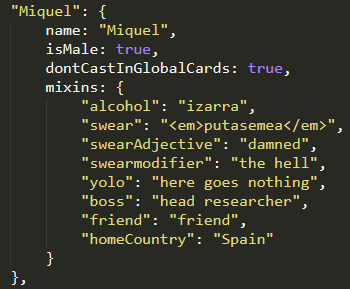
\includegraphics[width=8cm]{figures/2-Ice-Bound/casting-data.png}
    \caption{A character definition within the level definition file.}
    \label{fig:casting}
\end{figure}

%%%%%%%%%%%% END FIGURE %%%%%%%%%%%%%%%%%%%%%%%%%%%%%%%%

\paragraph{Level Definition.}\label{par:icebound-level-definition}

Level definition files are the heart of each level. They define characters, which symbols are available where, and all the art and music files. While the specifics of what values each one would have takes some time to develop, overall these were fairly lightweight to work with. The majority of their contents are actually concerned with the visual appearance and arrangement of items on-screen for the level, and therefore don't come into play as much during the content authoring stage.

We would also define here any custom ``mixins" that could be used by state templates to customize story text to fit particular characters. For example, in an event card about a confrontation with an authority figure (the ``boss" mixin in Figure \ref{fig:casting}) that might be a ``head researcher" in Miquel's case, or a ``government official" or ``naval captain" for different characters.

\paragraph{Cards (Symbols, Events, Endings)}\label{par:cards-symbols-events-endings}

What we call ``cards"---the individual units of content for the digital story in \textit{Ice-Bound}---were the main focus of authoring. The amount of overhead for writing a card was fairly low: one could start by writing a card statically-cast to a certain character, with static text, then go back in and start adding more dynamism progressively, until either the cognitive overhead was too high, or the desired complexity was met. In the case of the former, more cards could be added with conditions to help cover the possibility space between an associated group of cards.

%%%%%%%% BEGIN FIGURE %%%%%%%%%%%%%%%%%%%%%%%%%%%%%%%%%

\begin{figure}
    \centering
    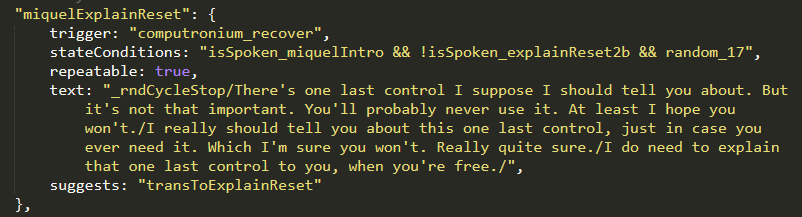
\includegraphics[width=\textwidth]{figures/2-Ice-Bound/dialogue-data.png}
    \caption{Sample JSON from an event card, with character and state templates.}
    \label{fig:dialogue-data}
\end{figure}

%%%%%%%%%%%% END FIGURE %%%%%%%%%%%%%%%%%%%%%%%%%%%%%%%%

These dynamisms could compound to become rather complex. In the example of Figure \ref{fig:dialogue-data}, we can see simple pronoun grammars, but also ones like \newline
``\_socket/miquel5/traitAdjective/." Because each symbol card comes with an associated adjective to describe the character, such as ``lucky" or ``foolhardy", this means you can reference that trait in subsequent cards, as long as we can ensure that character is cast. Because the template refers to a specific socket ``miquel5", which (perhaps somewhat confusingly) is always in Stanley's room, and Stanley is always cast as ``character a", we know by design that this will always line up.

Another interesting use of templates in this card is ``\_socket/miquel4/itemNoun/", which takes the symbol card's object, and inserts that into the text. Since the socket ``miquel4" in this case is a global symbol card, and symbols are always objects, we can get a nice spread of interesting things that Stanley keeps hidden away, and whoever is cast as character b can discover by picking the lock on their room.

While in terms of the discretely different things to be written for one piece of content is relatively low, this example shows how more complex and interesting permutations can be quite labyrinthine to craft. Often for these more complex cards, we would start with a premise (``an event where a character breaks into another's room and sees what's in there") and work from there, as opposed to writing static text, and then making it more generative afterwards.

\paragraph{KRIS Dialogues.}\label{par:kris-dialogues}

%%%%%%%% BEGIN FIGURE %%%%%%%%%%%%%%%%%%%%%%%%%%%%%%%%%

\begin{figure}
    \centering
    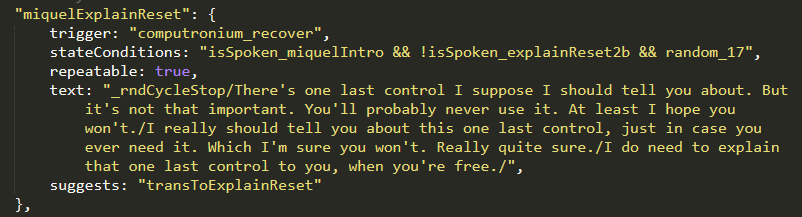
\includegraphics[width=\textwidth]{figures/2-Ice-Bound/dialogue-data.png}
    \caption{A sample KRIS dialogue.}
    \label{fig:kris-dialogue-data}
\end{figure}

%%%%%%%%%%%% END FIGURE %%%%%%%%%%%%%%%%%%%%%%%%%%%%%%%%

The branching dialogues with KRIS were similarly simple to create. Triggers and state conditions controlled when they appeared, which could come from player actions such as activating a symbol, other dialogues being triggered, or even randomly with a given percentage (shown in Figure \ref{fig:kris-dialogue-data}'s stateConditions as ``random\_17"). This text could be made more dynamic later on by going in and adding state-driven templating, or even just random variances for recurring dialogue prompts (as seen in Figure \ref{fig:kris-dialogue-data}). These dialogues could chain immediately to the following one by id, through the field ``suggests." They could also contain an ``options" array which would route the player accordingly once they picked the corresponding choice.

\paragraph{Book Pages}\label{par:book-pages}

Book pages were straightforward to create, being composed of static text or graphical elements, and then a secondary AR element. While they did have themes and tags applied to them, they were more authored as static conceptual narrative support for the digital narrative, to provide longer context and clues for what was going on when KRIS had written drafts of these stories while human. Writing this type of content required equal parts traditional narrative skills, as well as graphic design skills (for layout and design). This proved no problem for the authors, as they could leverage their common professional skillset from previous work as graphic designers.

\subsubsection{Clarity}\label{par:icebound-clarity}

Given the different layers of combinatorics between symbols, events, endings, KRIS dialogues, and theme resolution within the printed book, \textit{Ice-Bound} has complex system dynamics, although each individual piece on its own doesn't pose a particularly high degree of challenge. While it wasn't usually the case that newly authored content could modify state in such a way that necessary later cards were invalidated, the space needing content coverage was complex enough that tools were necessary in order to be sure that we had written enough content to account for all the different combinations of symbols a player may activate in the course of a playthrough. This is the area where we chose to spend most of our labor, in order to reduce the authorial burden. Without assistance here, the authoring task would have become too opaque for us to make consistent progress, and we would have no clear idea of when we had authored enough content to ensure the game was playable.

To avoid that, we essentially wanted to know two things: 

\begin{enumerate}
    \item How many combinations are needed for state coverage without an unattainable amount of writing?
    \item How can we know when we've accomplished coverage for all cases?
\end{enumerate}

In the course of development, we created three different content library visualization approaches to answer these questions. Because they are a bit involved, we'll first talk briefly about previous work in this area, in order to contextualize our decisions.

\paragraph{Historical Visualization Approaches}\label{par:historical-visualization-approaches}

Visualizing possible states the player may explore in a given piece is an authoring problem that’s been addressed in a number of different ways. The most prevalent visualization for interactive narratives is the simple graph (including trees), where nodes are individual story segments (or lexias) connected via the afforded actions of the player. Hyperfiction, for instance, typically uses the display of node connections to show the afforded action of clicking a link. These graph visualizations have been in place since the early days of non-linear storytelling with tools like Aquanet \cite{shipman1999spatial} and Storyspace \cite{bernstein_2007}, and continue to be used today in a variety of authoring tools, from Twine \cite{klimas2008twine} to game modding tools like the Neverwinter Nights toolsets \cite{nwnwiki_2019}. 

These sorts of graphs fill the most immediate need of authors: seeing the overarching structure of a piece, providing a way to see where paths of interaction dead end, where concentrations of links make certain content more likely to be displayed, or the lack of links makes it perhaps impossible.

As said by Mark Amerika, author of Grammatron: ``creating complex hypertext structures for the web is a nightmare because, after a certain point, one cannot visualize a cognitive mapping structure for a webwork that has literally thousands of screens and links" \cite{bernsteinamerika}. In this case, Storyspace’s ability to provide a simple spatial representation of reader pathways proved invaluable to his efforts. Another interesting aspect of tools such as Tinderbox \cite{tinderbox} and Twine, is that the authoring interface can be heavily bound up in the visualization itself, where creating a new node in the visualization directly maps to creating a new node in the work. Semantic flags in the writing itself can create new nodes, which are immediately added to the visualization. In these sorts of environments, the authoring is done from within the data visualization of the media artifact rather than as a response to experiencing the game or text, which (through leveraging good UI design) can dramatically increase an author’s ability to architect complex narrative structures. 

Games that provide powerful tools for the creation of new narratives with game engines, such as the Neverwinter Nights toolsets, still hold to the graph structure for narrative visualization, if they provide one at all. The well-used tree map for branching dialogue with NPCs is still the standard, and well-suited to most forms of menu-driven interaction with game characters. But it also begs the question: with different, more sophisticated visualizations, what narratives could become feasible to create?

Another visualization tool for interactive narrative debugging is the IDE for Inform 7, a parser-based interactive fiction language, which features a view of possible story traversals called the ``Skein." This mode also makes use of a graph metaphor, although with the graph now showing multiple playthroughs of the interactive narrative, which can be replayed upon changes to the narrative code to ensure they still produce the expected output. This opens up interesting diagnostic affordances to authors, allowing them to zero in on specific series of actions taken by players \cite{reed_inform}. However, this visualization has trouble addressing IF’s sheer combinatorial scale. The basic player affordance to interact via an arbitrary combination of nouns and verbs (``get lamp", ``drop lamp", ``light lamp") quickly becomes too large to be tenable for visualization, and would even perhaps not be considered useful. In general, it isn’t sensible to author dedicated content for nonsensical parser commands, such as ``eat lamp." Therefore, the easiest way to generate data for visualization falls back to playtraces, which can rely generally on players to engage in goal-directed play that avoids nonsensical parser command combinations.

Continuing in this vein, research into aggregating playthrough data into playtraces (such as Liu et al's work \cite{playtraces}) provides representations that could be adapted to provide narrative diagnostic strategies for projects where readers have a high level of expressive affordance. For example, Osborn's \textit{Gamalyzer} \cite{Osborn_playtracer} generates graph structures where certain nodes are defined as goal states, and each choice or state the player can induce in the system is a node connected by the action to the previous state. This emphasis on player actions as opposed to game states is well-suited for adaptation to narrative concerns, where many times the focus is on the variety of available player actions or affordance.

There have also been playthrough visualizations used for interactive narratives to better understand the potential space explored through interaction. For \textit{Prom Week}, a game making use of cutting-edge persistent social state modeling to create dynamic experiences for each player, visualization served a critical evaluative purpose in exposing how quickly individual playthroughs become unique \cite{promweek_playtraces}. These same techniques were used to demonstrate a similar property in \textit{Façade}, an earlier work famous for its expressive player affordances.

\paragraph{Design Goals}\label{par:icebound-design-goals}

The goal of the visualization system was to highlight where symbol combinations did not trigger at least three events and two endings, our self-selected minimum requirement for content. Symbol combinations where this is not the case needed more authoring. This metric was also parameterized, such that we could make it stricter later on in the authoring process, to provide finer feedback. When considering where new content would be most useful, the primary consideration was discovering a combination of symbols to be used as a precondition that filled existing holes in the possibility space. The visualization needed to provide information to allow authors to intuitively grasp how to accomplish that. \textit{Ice-Bound}’s engine is written in Javascript, so the visualization tool also needed to run on the same code base. This was necessary to minimize errors that might be introduced through re-implementation of game procedures, and also to ensure any future changes introduced to those game procedures would be faithfully reflected in the visualization. Ideally, the tool would both provide a window on the possibilities for an example level build (where all the symbols have been selected for sockets) and reveal possible level builds where there were not enough events or endings written or triggered, if certain symbols were involved. Furthermore, showing us which specific symbol combinations give rise to these states would give strong indicators for authoring appropriate preconditions to new events and endings in order to fulfill our goals.

\paragraph{System Description}\label{par:icebound-system-description}

The system was designed in two parts: a combination browser and a level profiler. The browser is concerned with broadly classifying combinations which need content, abstracted from a specific level build. The profiler gives a detailed view into the combinations within a specific level build. In operation, the combination browser is used to provide a list of explicit symbol combinations where content is sparse. The user can then click those combinations to build a level containing the given symbols, and through the level profiler, see how much content is needed to fix the scarcity issue.

\paragraph{Combination Browser}\label{par:icebound-combination-browser}

The combination browser engages all possible symbol activations for a level by permuting every unique combination of symbols from the global pool and level-specific pool of symbol cards, equal in length to the amount of available ``lights" on the level (the objects players manipulate to activate symbols) as specified in the levelDef file. It then uses the game logic to simulate activating each symbol, rebuilding the level if necessary to contain those symbols. If the level cannot be built with a particular combination of symbols (i.e. a symbol has a precondition precluding it being chosen if another symbol is present) it discards the combination as illegal. After each activation of symbols on this simulated level, the system records the number of events and endings activated.

Once the system has permutated through all valid symbol activation combinations and constructed this exhaustive list of events and endings, it decomposes the combinations such that it has a record of how many under-authored combinations each symbol is part of. For example, if the symbol combinations A, B, C and A, C, F both lack the appropriate number of events and endings, the system would yield that both A and C are part of two problematic combos, while B and F are only part of one.

This analytical strategy was chosen because the most direct solution to the problems highlighted by the viz is authoring more event and ending cards, with preconditions containing the specific symbols suggested. Thus, a symbol's presence in more than one combination inadequately covered by content is a good candidate for a precondition in future content.

Again, our goal is to increase system dynamics clarity for authors. Therefore, an important quality of this visualization is that it happens quickly enough to make it useful for making small changes and seeing how that affects the possibility space. Furthermore, once formulated, the data in the visualization can be quickly manipulated, which greatly increases its utility.

%%%%%%%% BEGIN FIGURE %%%%%%%%%%%%%%%%%%%%%%%%%%%%%%%%%

\begin{figure}
    \centering
    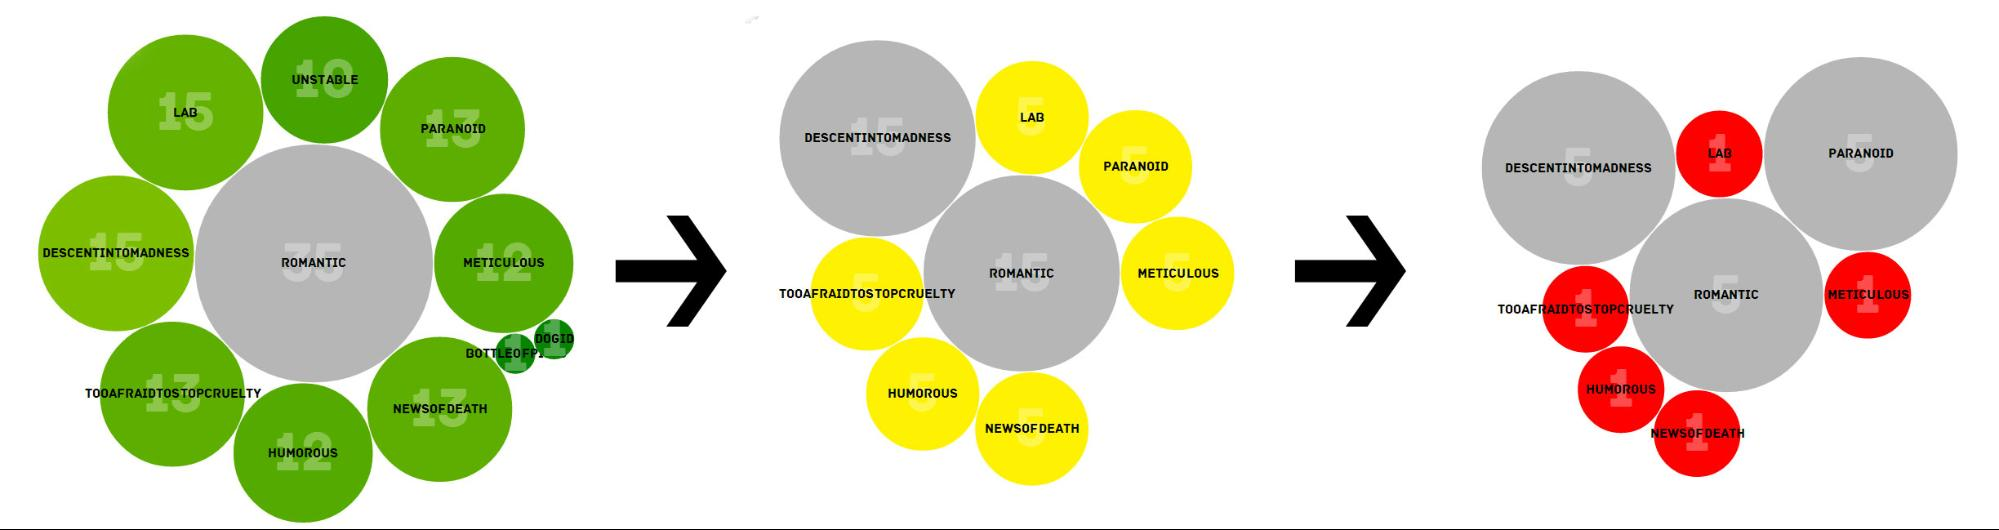
\includegraphics[width=\textwidth]{figures/2-Ice-Bound/bubble-viz.jpg}
    \caption{The combination browser, as the viewer progressively zeros in on problem combinations by clicking the symbol ``romantic", then ``descentIntoMadness", then ``paranoid."}
    \label{fig:bubble-viz}
\end{figure}

%%%%%%%%%%%% END FIGURE %%%%%%%%%%%%%%%%%%%%%%%%%%%%%%%%

\paragraph{Display Strategy}\label{par:icebound-display-strategy}

The browser displays each symbol as a circle in a bubble cluster diagram (Figure \ref{fig:bubble-viz}). The size of the bubble corresponds to the number of problematic combinations the symbol was involved in. Each bubble can be clicked to tell the system to apply the same visualization methods on the subset of combinations involving only the selected symbol. Doing this resizes the other bubbles in the visualization, so their new size corresponds to the number of times they are involved in a problematic combination with the new set of selected symbols. If a different bubble is clicked, the values are again updated. This allows the viewer to interactively evaluate and discover problematic symbol combinations.

There is a specific tension in authoring goals when trying to patch content holes. On one hand, the more combinations an authored event or ending hits, the more effective it is at patching a hole. However, if its pre-conditions mean it is also being activated for combinations which do not need more events and endings, it is potentially diluting that space. During gameplay, if a combination triggers more than five events or three endings, we truncate the list in order to keep the scope of the stories presented to the player from becoming overwhelming. However, the ranking policy we use to determine which to cut is very simplistic; additionally, there's always the risk that the ones we cut have an implicit connection to the symbols that is reflected in the authored surface text, but not reflected in nuanced ways in the content tags. If such events or endings are cut, it's possible it could lessen the perceived causal link between the player's choices and the system's response. Therefore, the closer we can keep all combinations to five events and three endings, the less we need to cut, and the higher the perceived causal link for the player from their actions to the reaction of the system.

To reflect these tensions, a ``traffic light" circle color scale from green to red was adopted to show the ratio of combinations needing content versus not needing content. Red circles have the highest ratio of content-less combinations, and green circles have the least. This is necessary in order to discourage the authoring of content with pre-conditions that trigger for combinations that don't need it. For example, while authoring an event with pre-conditions that trigger for every combination in the game would technically address every combination needing content, it would also appear for many combinations that didn't need additional events and endings. Also, from a narrative design standpoint, the more targeted an event or ending is to its precondition symbols, the better. It leads to content that strongly correlates with the player's selection, communicating that their choices are having a real effect, and that they have agency over the story being formed. Events or endings that show up for many different combinations are also more likely to conflict in some way with other content that is selected.

This means that the author can quickly browse to symbol groups that both have a high content need in their combination sets (by selecting circles with redder color) as well as representing a large number of the total combinations needing content for the level (by selecting circles which are larger).

Because the specifics of this are difficult to grasp, there is an additional info panel that displays the same information as the color and size, using text and tooltips (Figure \ref{fig:viz-detail}). The color, which is determined by the ratio of combos needing content, is reflected as a pie chart (C) with explicit text (B). The size of the circle is also shown numerically (D).

%%%%%%%% BEGIN FIGURE %%%%%%%%%%%%%%%%%%%%%%%%%%%%%%%%%

\begin{figure}
    \centering
    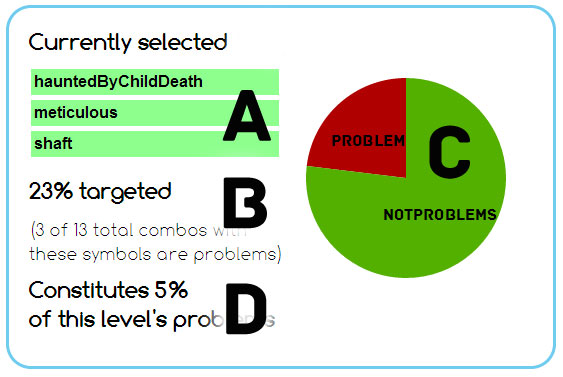
\includegraphics[width=\textwidth]{figures/2-Ice-Bound/viz-detail.jpg}
    \caption{The detail panel in the combination browser, showing the selected symbols (A), and the percentage of their combinations which need content (B), also represented by the pie chart (C). (D) shows how many of the total combinations needing content the current selection is involved in.}
    \label{fig:viz-detail}
\end{figure}

%%%%%%%%%%%% END FIGURE %%%%%%%%%%%%%%%%%%%%%%%%%%%%%%%%

While providing a good top-down view of the content distribution as a whole, the combination browser does not show the content distribution within run-time combinations of a particular level build. This gives rise to a blind spot in authoring considerations. If the combinations lacking content are concentrated in a few specific builds of a given level, that is a bigger problem than a low number of problems that persist across all possible level builds. For example, if only 1 out of 35 content-lacking symbol combinations is present in a level build, it isn't as glaring a problem as all 35 problems being present in one level build, due to the fact that a given level build can have around 30-70 combinations. In the first case, only 1.4 - 3\% of the player's possible chosen combinations are lacking. In the second case, it's closer to 50 - 100\%.

To address that, we needed a visualization dealing with specific level builds, accessible via the combination browser. This is accomplished through listing out the symbols currently being inspected by the viewer. If the symbols ``romantic", ``descentIntoMadness", and ``paranoid" are selected, the list contains every content-needing combination containing those symbols, with a link to ``build." When clicked, the system builds the level containing those symbols, and displays the second visualization tool: the level profiler.

\paragraph{Level Profiler}\label{par:level-profiler}

The level profiler (Figure \ref{fig:bar-viz}) was the visualization most used during the initial round of authoring for \textit{Ice-Bound}. It displays the run-time combinations of a given level build with a given set of symbols in the form of an annotated stacked bar graph. Each bar represents a particular set of active symbols, with the height corresponding to the total number of events and endings it activates.

%%%%%%%% BEGIN FIGURE %%%%%%%%%%%%%%%%%%%%%%%%%%%%%%%%%

\begin{figure}
    \centering
    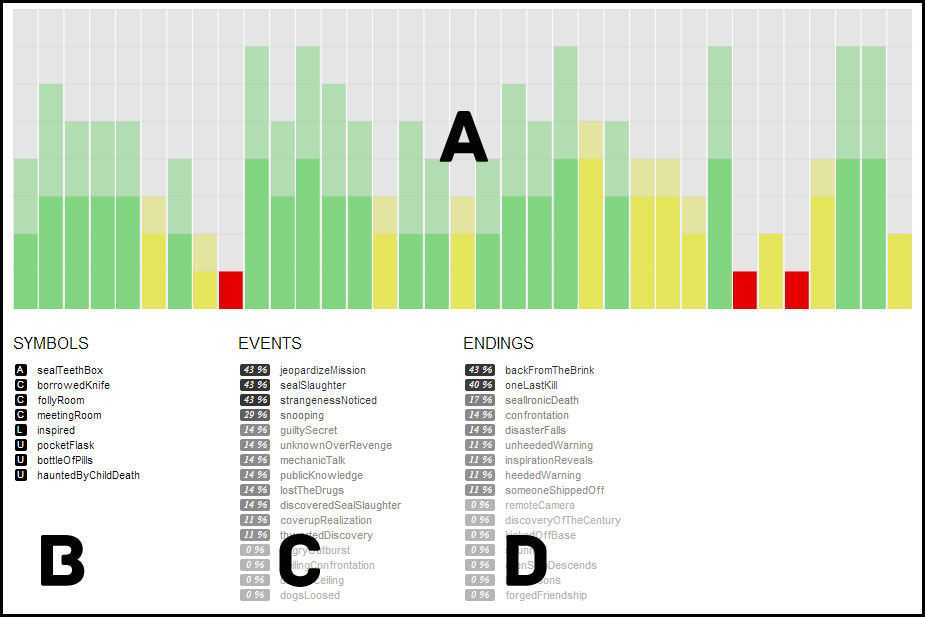
\includegraphics[width=\textwidth]{figures/2-Ice-Bound/bar-viz.jpg}
    \caption{The level profiler for \textit{Ice-Bound}, showing all possible run-time combinations of active symbols for a single build of a level. Red bars indicate content-sparse combinations. Clicking on specific Symbols (B) Events (C) or Endings (D) will re-sort the graph (A) to lump combinations using those cards together.}
    \label{fig:bar-viz}
\end{figure}

%%%%%%%%%%%% END FIGURE %%%%%%%%%%%%%%%%%%%%%%%%%%%%%%%%

The bottom portion of the bars represents events, and the upper portion endings. This provides an easy way to see which combinations do not trigger enough content. The coloration of these bars is either green, yellow, or red. This is dependent again on the two combination minimums we established for a ``satisfying" story: a combination should trigger at least three events and two endings. If a combination satisfies both of those, it is green. If it only satisfies one, it is yellow. If it satisfies neither, it is red.

Below the graph are a list of the symbols present in the level, as well as every event and ending that can be logically triggered by those symbols. Hovering over a given bar in the chart highlights the symbols, events, and endings activated in the lists below. Additionally, each item on the lists below the chart can force a re-sort of the chart upon being clicked. This means if authors want to see content authored for a specific symbol, event, or ending, they click on it, and the graph re-sorts so that all combinations involving that move to the left.

This proved enormously useful in highlighting problems that weren't readily apparent from the complex interactions of pre-conditions for various events and endings. Red bars indicating problem sets of active symbols could be examined to look for common elements, indicating there were not enough events and endings activated by those elements. Using this tool, one could quickly see what the combinations that need more content have in common, and get a feel for how much content is currently available to the reader at run-time. In this way, clarity for authoring was greatly increased.

\paragraph{Pragmatic Tables}\label{par:pragmatic-tables}

In addition to these data visualizations, which took a significant amount of time to build out, test, and deploy, we also used a ``quick and dirty" method to audit combinations. This took the form of a webpage that displayed several tables.

%%%%%%%% BEGIN FIGURE %%%%%%%%%%%%%%%%%%%%%%%%%%%%%%%%%

\begin{figure}
    \centering
    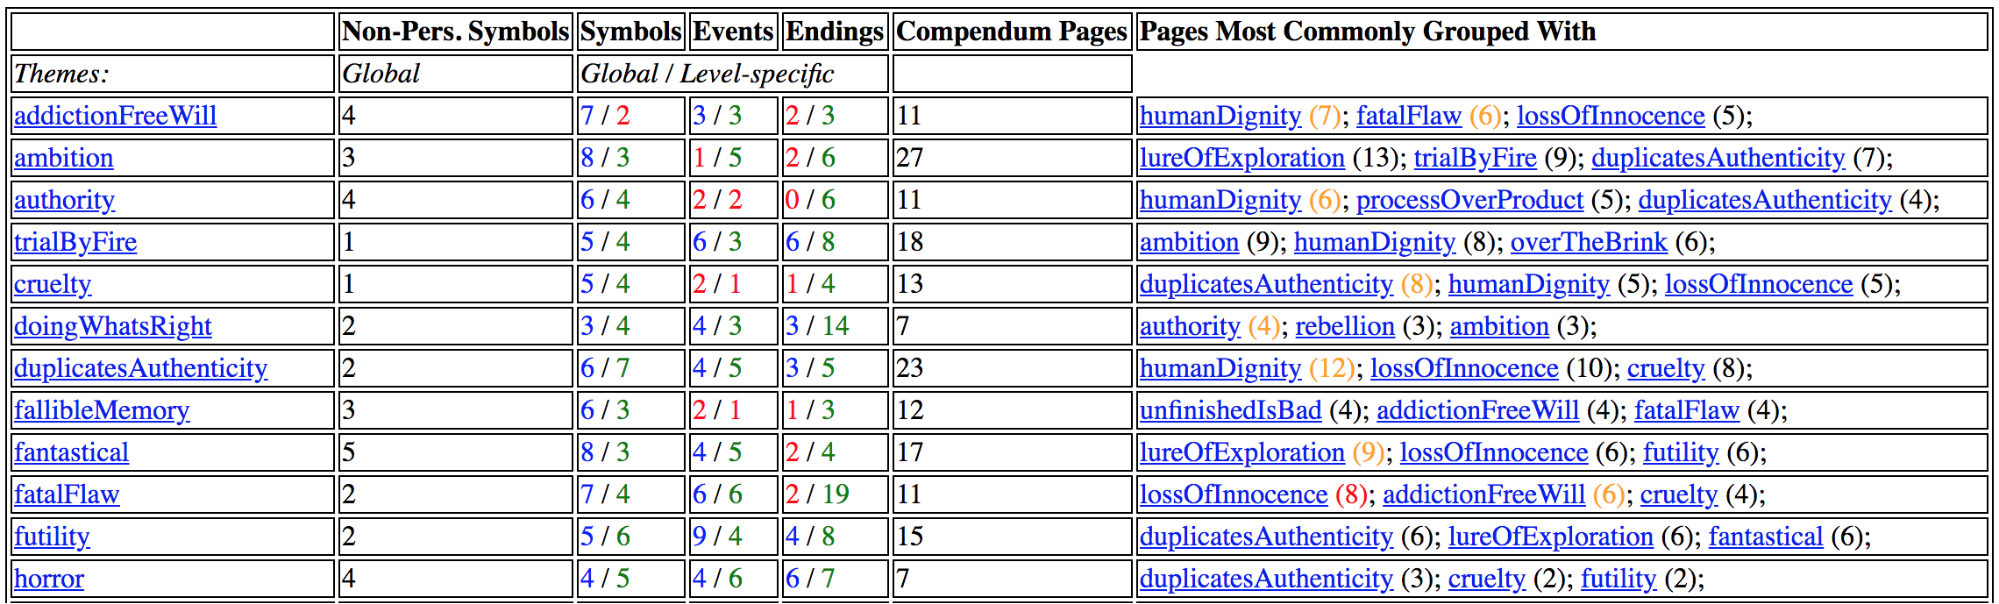
\includegraphics[width=\textwidth]{figures/2-Ice-Bound/pragmatic-tables.png}
    \caption{A table selection showing themes, as well as how many symbols, events, and endings use it.}
    \label{fig:prag-tables}
\end{figure}

%%%%%%%%%%%% END FIGURE %%%%%%%%%%%%%%%%%%%%%%%%%%%%%%%%


As seen in Figure \ref{fig:prag-tables}, each theme is listed, along with how many global or level-specific cards implement that theme for the three types of content cards. Numbers are color-coded red when there is less than a viable amount written. This makes it simple to see at a glance which themes are most in dire need of content.

This same page also has a simple text listing of ``pages with fewest themes", ``tags/themes most used as preconditions", ``tags/themes least used as preconditions", ``cards most used as preconditions", and ``cards least used as preconditions", arranged from highest value to lowest value. This provided us a barebones way to avoid over-using themes, which as mentioned in discussion of the more elaborate visualization, dilutes their perceived effectiveness to the reader.

%%%%%%%% BEGIN FIGURE %%%%%%%%%%%%%%%%%%%%%%%%%%%%%%%%%

\begin{figure}
    \centering
    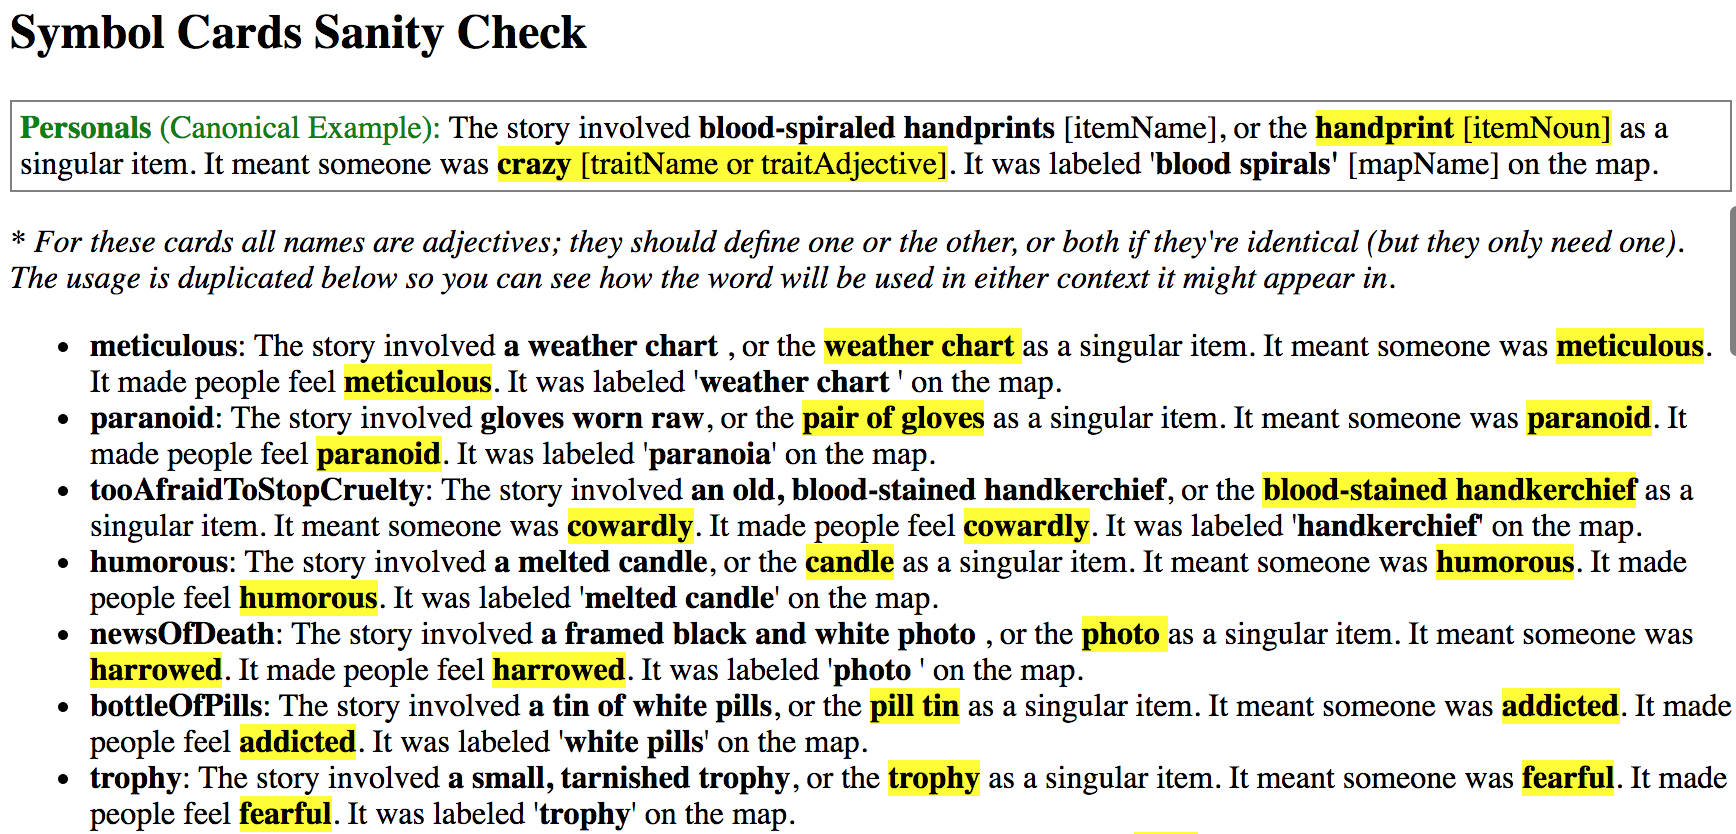
\includegraphics[width=\textwidth]{figures/2-Ice-Bound/symbol-checker.png}
    \caption{Rendered text for symbols, to check for coherence.}
    \label{fig:symbol-checker}
\end{figure}

%%%%%%%%%%%% END FIGURE %%%%%%%%%%%%%%%%%%%%%%%%%%%%%%%%

A separate section displayed all the ways a symbol card could be used in a sentence. This let us audit the creation of new content that might be combined in surprising ways, to ensure it would remain grammatically correct regardless of where it appeared.

\subsubsection{Controllability}\label{subsubsec:icebound-controllability}

The Controllability requirement for \textit{Ice-Bound} was, taking all things into consideration, roughly Medium. Despite the firm target of at least three events and two endings for every combination in the level, we were helped by the aesthetic decision to keep story segments relatively self-contained (which is reflected in the Medium level of Contextuality). This meant that surprising juxtapositions could be plausible explained by the reader as long as the leaps weren't too far, keeping in mind the design mantra of Failbetter's ``fires in the desert." The level profiler and combination browser visualizations here also allowed us to quickly browse through existing combinations, to find situations where badly written preconditions resulted in strangely triggered (or mis-triggered) events and endings. All in all, most events and endings in \textit{Ice-Bound} are adequately controlled by pre-conditions with just three to five terms, all of which are simple booleans checking for the activation of other cards or certain tags.

In terms of the surface text (and in order to support surprising juxtapositions by providing some supporting consistent details) we did want to exert strict control over the casting of characters. This was both to ensure their role persistence through the stories aggregated from the triggered cards, as well as their dominant qualities, since the stories were, aesthetically speaking, predominantly character studies. This we accomplished with the aforementioned DSLs and state-driven templating. However, we also were able to reduce authorial burden here by framing some tricky templating instances as shimmer-text, which allowed us to both showcase the potential variant space while providing a piquant user interaction, while also freeing ourselves from the need to track more variables to do it automatically. This quality parsimony, to borrow another term from Failbetter, also helped keep things relatively simple and increase authorial Clarity as we created content.

\subsubsection{Authorability Summary}\label{subsubsec:icebound-authorability-summary}

Of the three main projects discussed in this dissertation, \textit{Ice-Bound}'s authoring tools were the most well-developed by far. Relatedly, \textit{Ice-Bound}'s content creation system was also the one most ``put through its paces" to create a shippable narrative experience, both in terms of volume and quality.

Because the state and system dynamics of the experience were complex, these different approaches and strategies each provided a lens we could use as authors to increase Clarity, by simplifying those dynamics to either an integer in a list, or a simple visual representation of circles and colors. Also, negative feedback was prominent enough that when content was made that had bad dynamics, it was immediately obvious.

These tools were run continuously throughout content creation for the process, and could give feedback immediately. Because of this, it was easy to create a "todo list" of cards for a given writing session, with specific constraints which---while at a given point the writer may not know how it fits into the bigger picture---mean they will be increasing our content pool as efficiently as possible. The distillation of this was our one sentence prompt at the top of the tables page, which might read something like ``Why don't you write an event or ending card about theme\_ambition (5) triggered by tag\_mazeMemory (1)?"

Towards the end of the writing process, the increasingly-specific constraints took on a form of writing under constraint (reminiscent of the aforementioned Calvino work \textit{Mr. Palomar}) which was actually more of a pleasant challenge than an onerous or confusing burden. Even if the writer came to the table with a certain event or character development they wanted to use, they could then say ``how can I change this such that it's also about ambition, or rebellion." And if a given thematic combination was too difficult to author, these visualizations allowed us to easily find alternate ways to satisfy the requirements using different thematic combinations, despite the complex dynamics at play.

Thus, despite the Complexity being fairly high for authoring content, it was ameliorated by the Clarity afforded by our feedback solutions. Because of aesthetic decisions that meant each card was relatively self-contained, and the aforementioned visualization tools, we could get away with a roughly medium amount of Controllability. And because the Proficiency required for authoring was evenly matched with the author's skills (easily achieved, since we were the only authors!) the net result was a design and creation process with high authorial leverage.

\section{System Summary}\label{sec:icebound-system-summary}

\textit{Ice-Bound} was a successful project, from conception to finished media experience, because we managed to thread the needle of runaway combinatorial authorial burden with solutions to curtail it, and make the content needed for our systems pull double-duty. Our initial concept of the project was one that would require high Traversability. Because of the time invested in paper prototyping and iterating on simple digital prototypes, we were able to zero in on the key ways we wanted the system to shine: high Explorability (through the ``sculptural fiction" mode of interaction) and Replayability, through the use of high Contextuality. In order to help meet that challenge, we put in place designs from the beginning that would help reduce the amount of authoring needed by increasing content Reusability, through card availability in multiple contexts, and cards fulfilling multiple spots in the content library for different sets of preconditions, assisted by the state-driven templating.

In order to meet this content creation challenge, we needed to increase our Authorability as much as possible. Because the content authors were also the system engineers, we were able to get away with a relatively high requirement for Proficiency, while still having the friction for authoring remain fairly low. The many different components required for authoring (cards, KRIS dialogues, Compendium pages) pushed the Complexity high.

However, because of the amount of effort spent on tools---from the simple-yet-informative ``pragmatic tables" to the more exhaustive combination browser and visualizer---we were able to increase our Clarity greatly. These tools enabled us to zero in quickly on bad dynamics or holes in our content library, and also determine when we needed to find ways to increase the reusability of particular pieces of content, and when we needed to simply roll up our sleeves and get to work.

\section{Next}\label{sec:icebound-next}

\textit{Ice-Bound} was a successful endeavor, from both a research and media production standpoint. However, many things were already working in its favor. And while it was still an experimental work by many metrics, many of the decisions made in its development ``reigned it back" in service to releasing a finished product to a waiting audience. Features were cut early on, capabilities that could have pushed the procedurality further were left for ``the sequel" (a facetious phrase we used to make the parting easier) ensuring we could finish a polished work using the system.

Next, we turn to the familiar domain of choice-driven narratives. Driven this time more by a research mandate for the creation of a novel system with a wide array of experimental narrative affordance, we were able to push the boundaries a bit further. The result was a system that advances the evolution of dynamically-assembled choice-based narrative, but fought against ever-escalating authorial complexity. In the course of that fight valuable insights were gained, both in system architecture and narrative design, and resulted in both a publicly available narrative engine, and a finished research game: \textit{Emma's Journey}.


\chapter{StoryAssembler}
% \section{section} (h2)
% \subsection{subsection}
% \subsubsection{subsubsection}
% \paragraph{paragraph}
% \subparagraph{subparagraph}


StoryAssembler is an engine for dynamically generating choice-based narratives. It has a high degree of expressive capability, enabling collaborative authoring of dynamic choice-based narratives by first-time authors. It culminated in the release of both an experimental research game (\textit{Emma's Journey}) as well as an open-sourced library which hopefully will be used in future projects.

%%signposting%%
As with \textit{Ice-Bound}, we'll start with detailing the specific experience we were trying to create. For StoryAssembler, this was a dynamically generated choice-driven narrative, which was reactive to the player in novel ways. Then, we'll detail some related systems and works in the area of hyperfiction (Section \ref{sec:sa-hyperfiction}), planner-driven narrative (Section \ref{sec:sa-planner-refs}), and generative choice-based narrative (Section \ref{sec:sa-gen-choice-refs}). Taking these features and characteristics into account, we'll then do a deep dive of the system architecture and capabilities, as well as implementation-specific features for \textit{Emma's Journey}. This will provide us with the necessary context to discuss the authoring challenge for \textit{Emma's Journey} as it applies to the Authorial Leverage Framework. Namely: a narrative framing with high Contextuality requirements means also a high degree of required Controllability, which if not mitigated can make authoring even modestly-sized works very challenging.
%%signposting%%

\section{Experience Challenge}
\label{experience-challenge}

\textit{Emma's Journey}, the flagship experience for the StoryAssembler system, was planned as a ``serious game" focused on the urgent topic of climate change. As a pedagogical category, ``serious games" is somewhat amorphous and variegated, encapsulating everything from edutainment to military simulations, depending on the use case. Abt, when describing the educational use of analog games, defined it in 1970 as those which have ``an explicit and carefully thought-out educational purpose and are not intended to be played primarily for amusement" \cite{abt1970serious}. Interestingly enough, in the first paper on the subject published with Cogger in 1969 \cite{Abt_Cogger_1969} the two games used as exemplars deal with the topics of evolution and environmental sustainability, two challenging subject areas that unfortunately join climate change in current times as topics requiring sometimes considerable persuasive--in addition to scientific--skills to impart their lessons. Abt characterized serious games as good pedagogical techniques for communicating concepts through the compelling use of simulation, as opposed to traditional static means. Thus, the root of this approach speaks to the use of ``process literacy" as a way of gaining mastery over material, which we will return to shortly.

Years later, the term was translated (or unearthed) to apply to digital games, under the auspices of the Woodrow Wilson International Center for Scholars, who founded the Serious Games Initiative in 2002 \cite{serious_games_init}. In more recent years, Bogost has sought to rehabilitate the notion of ``serious games" as being overly bound to institutional mores by implication, and suggests as an alternate the more content-centered label ``persuasive games", such that it can encapsulate games which seek to challenge--not support--institutions \cite{bogost2010persuasive}.

Regardless, these types of games typically rely on techniques used in entertainment to build rapport with the player, and leverage that rapport to communicate knowledge players may find difficult to otherwise learn. For example, narrative framing techniques can be used to elicit sympathy from the player for a struggling protagonist, whether that's a struggling single mom trying to run a business in \textit{Cart Life} \cite{hofmeier2011cart}, or a harried border agent trying to walk the line between self-preservation and humane action in \textit{Papers, Please} \cite{pope_2012}. Or perhaps the player is engaged as a character in the narrative itself, blurring the line between game and reality, as with participatory transmedia ARGs (alternate reality games) like \textit{World Without Oil} \cite{eklund_mcgonigal_2007}.

Narrative is only one potential strategy, however, and has its limitations. While it can help make topics more relatable through players identifying with the characters, it can be harder to communicate rhetorical points of system dynamics, things that systems-based mini-games might accomplish more easily \cite{frasca2013simulation}. These games can oftentimes achieve their goals with little to no narrative framing, as with the serious games Abt originally outlined, but also in modern digital offerings such as with \textit{newsgames}, meant to provide an editorial opinion on a topic through the use of simple mechanics \cite{treanor2009newsgames}.

%%%%%%%%%% BEGIN FIGURE %%%%%%%%%%%%%%%%%%%%%%%%%%%%%%%%%%%%%%%%%%%%%%%%%%%
\begin{figure}
    \centering
    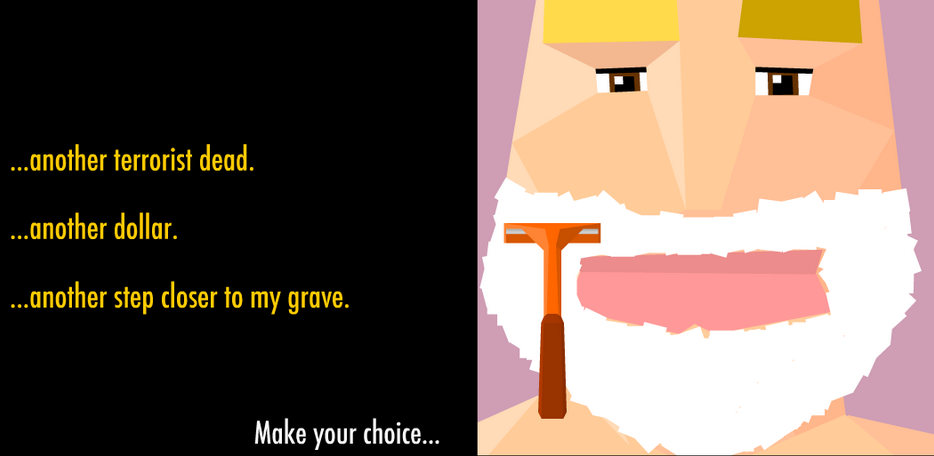
\includegraphics[width=\textwidth]{figures/3-StoryAssembler/unmanned.png}
    \caption{Screenshot from Molleindustria's Unmanned}
    \label{fig:unmanned}
\end{figure}
%%%%%%%%%%%%%%%%%%%%%%%%%%%%%%%%%%%%%%%%%%%%%%%%%%

Given this landscape, we wanted to investigate what could be accomplished by combining the two together, as a sort of simultaneous ``two channel" gameplay / narrative experience. One game that provided an inspiring potential blueprint to follow was Molleindustria's \textit{Unmanned} \cite{pedercini_jim_munroe_2012}, which follows the life of a remote drone operator through a series of vignettes pairing narrative and minigames. The game is highly successful in communicating the absurd juxtaposition present in the day-to-day life of a remote drone operator: shaving, driving to work, authorizing the remote killing of people via drone, then coming home and playing with his son, as a sort of interactive testament to the banality of evil. Each section is a different piece of the story paired with a mini-game that engages the player in a different way, most of them simple choice-driven vignettes (Figure \ref{fig:unmanned}). 

But while this two-channel experience has both mini-game and narrative, the connection between them doesn't extend deeply in a procedural sense. While there is ``gating" (if you perform badly in the game, the narrative vignette doesn't progress) there is no persistent connection in state or dynamics between the two. Choices you make in the narrative also do not impact the gameplay, so the connection is rather limited and one-sided.

Therefore, we wanted to create a two-channel game--one where a mini-game accompanied an ongoing choice-based narrative--and the two could influence each other not just in a lockstep way as in \textit{Unmanned}, but in a more granular, stateful way. Additionally (and most challengingly!) we wanted our system to be able to procedurally generate \textit{both the narrative and the mini-game}, working in unison in such a manner that it could accomplish the same types of rhetorical goals as seen in \textit{Unmanned} and other serious or persuasive games.

Structurally, these vignettes and games would need to be generated from generalizable lists of goal states and game dynamics. This was an initial design preference to accommodate potential future work, where a ``Coordinator" system could procedurally determine the goals for the scene, and from that extrapolate which goals should be sent to the mini-game and narrative sub-systems. As of the initial release of \textit{Emma's Journey}, these were left as hand-authored goals, although as detailed later in Section \ref{dynamic-story-specs}, we were able to inject some template-driven dynamism into them and expose them to the player, in order to provide some control over the starting states, and increase the sense of interactivity.

In form, the types of stories we hoped to create with StoryAssembler for this application were reactive choice-based narratives. Specifically, we wanted to design a system that could receive an input of a goal state, and craft a narrative that would hit all of our goal elements, \textit{no matter what the player chose}. It was hoped that stories created with this system could adapt to the way the player played them, providing an experience where the system's responsiveness would be apparent, but would still be hitting the rhetorical goals the author would encode into the story as goal elements. And through all this the narrative would be fluidly supported by the ongoing mini-game, which through their combined power, it was hoped, would powerfully address the topic of climate change.

\section{Related Works}

\subsection{Hyperfiction / Choice-driven Systems}
\label{sec:sa-hyperfiction}

StoryAssembler generates dynamic choice-based narratives, similar in output to hyperfiction. These types of narratives have also been with us in digital form for quite some time, with early systems like HyperCard \cite{hypercard} and Eastgate's Storyspace \cite{eastgate} creating a fertile initial ground. And their non-digital counterparts have of course been with us for quite some time, with modern choice-driven works like \textit{Choose Your Own Adventure} (CYOA) books and also the earlier dynamically assembled works touched on in Section \ref{subsec:ib-non-digital-combinatorial}.

Hyperfiction experienced a cultural revival of sorts with the rapid adoption and proliferation of Twine works in the early 2010s \cite{twinePlatform}, although there has been a steady stream of systems released throughout the years such as ChoiceScript \cite{choicescript}, Inkle Studios' Ink \cite{ink}, and Undum \cite{undum} (with its later enhancement, Raconteur \cite{raconteur}) to name just a few.

Similarly, there is a rich existing field of hyperfiction design practice, with a myriad of different works making use of their respective software's affordances to achieve various aesthetic effects through the structuring of their choices and links. Some experts have analyzed these choice-based authoring patterns in a more taxonomic and structured approach, such as Mawhorter's work on Choice Poetics \cite{mawhorter} (which we will return to later) and Ashwell's Standard Patterns in Choice-Based Games \cite{ashwell}. Such affordance analysis exists on top of the implicit design practice outlined in software-specific or studio-specific authoring guides also tackling the issue, such as with ChoiceScript \cite{choicescriptGuide} or InkleWriter \cite{inklewriterGuide}. 

StoryAssembler exists in the same family of output, in that its stories resemble those of these systems. However, the highest-level procedures it uses to generate choice-based narratives are planner-based, rather than explicitly coded by the author, which affords potentially richer and dynamic structures to be created, but requires far more complex structural design sensibilities.

\subsection{Planner-driven story systems}
\label{sec:sa-planner-refs}

In comparison to hyperfiction systems, which oftentimes rely on explicitly linked passages for much of their authoring, planner-driven story systems rely on heavier computational lifting to assemble their stories dynamically from a library of authored actions/operations. StoryAssembler's core is a forward state-space planner working in tandem with an HTN-like planner (which we will come back to in more detail in Section \ref{core-architecture}). These qualities put StoryAssembler in line with threads among the planner-based story generation community, a broad swath of research which stretches back to systems such as Lebowitz's \textit{Universe} from 1983 \cite{universe}, one of the earliest examples of planning systems focused on plot generation. 

A useful characterization of narrative generation systems first by Dehn \cite{dehn} (and later applied specifically to planner systems by Riedl and Young \cite{planningRiedl}) is that of having two main approaches: simulationist and deliberative. Simulationist (or emergent) systems (such as Meehan's \textit{Talespin} \cite{meehan1977tale}, Cavazza et al's \textit{I-Storytelling} system \cite{cavazza2002interacting}, and Chang et al's \textit{Othello} \cite{chang2009planning}) rely on bottom-up rules for the world and characters to form the basis of stories, which emerge organically from the processes. In contrast, deliberative systems (such as Lebowitz's \textit{Universe} \cite{universe}, Turner's \textit{Minstrel} \cite{minstrel} and Pérez y Pérez et al's \textit{Méxica} \cite{perez2001mexica}) set up situations to be resolved (usually fulfilling some abstracted authorial goal) or desirable states posited to the system, which has a series of available actions it can take to effect state changes to reach the desired state. StoryAssembler takes the deliberative approach to generation, although it could be stretched to accommodate simulationist systems, by leveraging the mini-game state interface capabilities detailed in Section \ref{implementation-details}'s discussion of \textit{Emma's Journey}.

There have been a number of useful survey papers published on this wide-ranging field, such as Mateas's 1999 survey \cite{mateas1999oz} which focused on story generation in the context of believable agents, Roberts et al's 2008 survey with a focus on drama management \cite{roberts2008survey}, Arinbjarnar et al's 2009 survey with a focus on interactive drama systems \cite{arinbjarnar2009critical}, Goudoulakis planning algorithm survey dedicated specifically to Digital Interactive Storytelling \cite{goudoulakis_2011_survey} and Kybartas et al's 2017 excellent survey positioning planner-driven systems as a form of mixed-initiative storytelling \cite{kybartas_2017}. While the examples and projects are multitudinous, there are a few tackling the similar domain of choice-driven narrative are useful to look at in some depth to help position StoryAssembler's place within this milieu.

Additionally, it should be noted that historically, the media artifacts generated by many planner systems are often not as fully realized as ones generated by hyperfiction authors, as the primary computational research goal for planners can often be accomplished with simple sentences used as story beats, or even through re-purposing existing texts by breaking them into their component parts and procedurally traversing them, such as Yu and Riedl's work with CYOA books \cite{Yu}. It was important in the development of StoryAssembler that the focus remained on the final product being recognizably a choice-based narrative that could hold its own alongside more traditionally authored Twine-based hyperfiction, which necessitated a hybrid approach in system development. In some cases this meant starting from simple planning structures with little generativity that were easy to author, then adding in more robust and generative operations and states later on as part of the editorial process, which required more complex design thinking to achieve. The interplay between this is elaborated upon more in Section \ref{complexity}'s discussion of Complexity. That said, there are some systems that bear similarity in part to StoryAssembler that it is useful to inspect at greater length.

Barber and Kudenko's 2007 system is an early planner-driven choice-based narrative system, which forces players into dilemmas as choice points \cite{barber2007dynamic}. The writer in this case provides STRIPS-style actions and storyworld knowledge of characters, relations, and locations. For their initial world, following the lead of \textit{Universe}, Barber et al chose the domain of soap opera cliches, situating their stories in a mode where drama is high and unambiguous. The system then creates a sequence of actions that lead to a dilemma (such as ``personal gain versus loyalty to friend"). The dilemmas are authored with pre-conditions, and the system moves from dilemma to dilemma as long as possible, using actions to move the state such that it satisfies the dilemma's preconditions. The content for these is very light, and not to the level of a traditional narrative. The focus is rather on the composition of planner actions to generatively move through the state space. To this end, Barber explicitly states, ``Our goal is to keep the story designer’s input to a minimum and the user involvement as high as possible." A sample storylet might be something as simple as ``joe offers to buy you a drink. Do you accept?" While they maintain that longer narratives are possible by chaining together an appropriate library of content to move between dilemmas, there isn't an overarching narrative they are seeking to fulfill, as opposed to StoryAssembler's architecture.
%%GDoc comments%%
Planner-based interactive narrative generation is an active area of research to present day, with systems like Robertson et al's General Mediation Engine \cite{justus} in 2018 making strides towards parser-based generated narrative worlds. This engine iterates on Riedl et al's conceptualization of \textit{narrative mediation}, used to reconcile player agency and authoring constraints \cite{riedl_mediation}. Narrative mediation is made up of two approaches: \textit{accommodation} when the system changes to suit the player, and \textit{intervention} when it modifies the effects of the player's action to preserve the original constraints. Justus and Young then developed a method--called perceptual experience management--which rides the line between each by exploiting a model of the player's incomplete knowledge. This allows it to generate new narrative branches by changing past world events based on their PDDL (Planning Domain Description Language)\cite{pddl} representation. StoryAssembler is also concerned with dynamically changing choice-based narratives depending on player action, although the dynamism of the planner goals is a player-driven affordance, as explained in Section \ref{dynamic-story-specs} on dynamic goal states. Furthermore, while Robertson et al's system initially was textual, it later moved to a 2D Unity representation. This initial textual representation was also that of a parser-based interactive fiction work--where brief, functional descriptions of rooms are given, and player actions may be entered. In comparison, our choice-driven domain has more in common with Twine works of hyperfiction, where substantial thought must be given to the surface text displayed to the player.
%%GDoc comments%%
As a general characteristic StoryAssembler also differs from many narrative planners in that it diegetically surfaces parameterized planner operations to the reader through dynamic scene descriptions. This surfacing is shown in scene introductions, where players can read parameterized goal states as diegetic text, and alter them to suit their tastes before the planner executes to generate the story (more details on dynamic goal states can be found in Section \ref{dynamic-story-specs}). StoryAssembler is still tightly related to these other planners if one considers the potential generative space of their system output as a sort of ``choice-based'' narrative, where the planner makes the choices and then shows the resulting traversal to the player, instead of the player choosing from the myriad options at each step of execution. However, on the whole it is most useful to consider it in dialogue with narrative planner systems that afford interactivity from the player, and most specifically, choice-based works that require discrete moments of interactivity between a small number of options.

\subsection{Generative Choice-driven Systems}
\label{sec:sa-gen-choice-refs}

Procedural systems focusing on generating choice-driven narratives are a rarer niche within this area of literature, but StoryAssembler was developed in an environment where other concurrent threads of research were being developed targeting a similar medium, though with markedly different approaches.

\subsubsection{Dunyazad}

While StoryAssembler was first being conceived, a parallel project was continuing its development after springing from a common root of tackling climate change education through choice-based interaction: Mawhorter's Dunyazad, an Answer Set Programming-driven system for generating situational choices \cite{dunyazad}. 

Dunyazad is an operationalization of Mawhorter's theory of choice poetics \cite{dunyazad}, \cite{mawhorter_diss}, which seeks to model the structure of player choices in narratives. It does this by reasoning in terms of player goals, expectations and perceived outcomes. Player goals are assumptions explicitly coded by the author, such as ``the player will want to preserve their life as well as that of their allies." These goals are surfaced to the player in a scene introduction, priming them for the mode of engagement they should take. Mawhorter also distinguishes three modes of player engagement in his model: power play, avatar play, and role-play. These categories delineate players pursuing ludic goals, such as (respectively) a high score, making choices as if they are the character, or expressing a more abstracted role through potentially multiple characters.

Player expectations and perceived outcomes are both driven by a skill check system. The system reasons based on necessary skills for each action; the action is likely to succeed if the player possesses the requisite skills, unlikely to succeed otherwise. The post-conditions attached to each choice are then evaluated to see if the player would perceive the outcome as positive, negative, or irrelevant, given their goals.

A typical scene in Dunyazad consists of a setup to prime the player, plus some number of ``actions", which can either be choice nodes (where the player makes a choice) or event nodes (system-dictated bridging nodes for continuity). The surface text for these nodes, as with StoryAssembler, makes use of state-driven templating, to handle pronouns and other qualities. Nodes in Dunyazad consist of context (world state), pre-conditions, options (actions the player can take) and outcomes (post-conditions).

In contrast to StoryAssembler, Dunyazad can generate the entire choice graph beforehand, since it has no other process modifying the state blackboard outside it. It generates stories using a predicate representation that can handle story elements such as characters and items, then generates some number of options with an action associated with it along with argument bindings. It generates the graph by reasoning about desired poetics, with the goal of achieving particular effects. It composes groups of choices based on definitions from choice poetics, such as a ``relaxed" choice (low-stakes, with no adverse effects for any option), ``obvious" choice (one option that is clearly positive), and ``dilemma" choice (every option is equally undesirable).

However, the largest difference between Dunyazad and StoryAssembler is that StoryAssembler explores the broader challenges of narrative coherence and dynamic choice construction, as opposed to Dunyazad's tighter focus on the poetics of a set of options at a single choice point. Mawhorter notes that Dunyazad was an environment ``in which the poetics of individual choices (e.g., was the last choice relaxing?) are important to the feel of the story overall, as opposed to merely supporting a dramatic arc defined by traditional narrative elements" \cite{dunyazad}. Our motivation, in contrast, was geared towards how we could assemble fragments and their choices to \textit{support} a well-defined story and dramatic arc, while still being generative.

\subsubsection{Minstrel, Skald, \textit{Problem Planets}}

Mawhorter had previous experience with story generation, working on a generative narrative system with Tearse called Skald \cite{tearse_skald}. Skald was an attempt to rationally reconstruct--and then extend--the seminal work of Scott Turner's Minstrel system \cite{minstrel}, an early story generator famous for its case-based model of narrative creativity. Minstrel used case-based reasoning to assemble stories from a library, adapting them using methods called ``TRAMS" (transform-recall-adapt methods). Unexpectedly, upon successfully reconstructing the system, Tearse and Mawhorter were unable to reproduce Turner's output with any sort of regularity--in early tests of the system only 35\% of 1000 generated results could be deemed sensible \cite{tearse_results}. When they tried different settings to increase sensibility, it precipitated a collapse of the generative space such that only a handful of unique results were returned.

In Skald's case, the system evolution was driven, at least partially, by the concrete media experience \textit{Problem Planets}. \textit{Problem Planets} was an attempt to use Skald to generate narratives for different planets visited by the player, each with their own issues that needed resolving. The idea was that, through showing the player different ways to find solutions to these problems, it would encourage systemic thinking for the player about the real-life issue of climate change.

For this experience, a library of stories were written, paired with TRAMS and ALPs (author level plans). As the team struggled to bend the system to consistent output, they found themselves leaning more heavily on the ALPs to enforce sensible output. Additionally, trying to add new stories to the library to increase the system's expressiveness would frequently introduce new inconsistencies in previously-consistent stories, due to the combinatorial nature of Skald. Additionally, on top of all this was the need to provide interesting interaction in the form of choice points, so the player could determine the course of the story (similar to the challenge later set before StoryAssembler).

The team came to the conclusion that the authorial burden introduced by trying to author new content that wouldn't trigger unforeseen inconsistencies was too infeasible, despite the technical proficiencies and advanced narrative design capabilities of the writers (one member, Aaron Reed, was the co-author of \textit{Ice-Bound}). These challenges--an increase in authorial friction due to Complexity, coupled with a lack of Clarity for the state being written for--were similarly encountered with StoryAssembler, and are elaborated upon in Section \ref{clarity}'s discussion of Clarity.

This project, in a way, is a connection between Dunyazad and StoryAssember, as the project StoryAssembler was created to enable, \textit{Emma's Journey}, is a different, later approach to tackle the same problem: generative choice-based narratives focused around the theme of climate change education.

While certainly challenging, Skald was illuminating. Mawhorter's experience on that project working with authoring constraints for choice-driven narratives is part of what spurred him to create Dunyazad. And given Skald's results, we were very conscious going into development of \textit{Emma's Journey} to build with an eye towards controllability and reliable generation, so that we would be able to hit our communicative goals.

\subsubsection{Lume}

Finally (and most recently) the Lume system \cite{mason2019lume} is similarly motivated to StoryAssembler: its goal is to enable greater expressiveness and reactivity in fully-realized choice-based narratives through increased procedurality. In contrast to StoryAssembler, whose scenes are planner-driven to a goal state composed of several blackboard values (expanded on in Section \ref{system-description}) Lume adopts a model of dynamically constructed node-trees (Scenes) which are then strung together combinatorially based on constraint satisfaction when a given scene concludes. This interplay seeks to achieve a specific experience for the player. While within scenes, the choice and template-driven dynamism surfaces the system state. Content is designed such that, at the conclusion of a given scene, it's intended a player should feel they have made choices that are distinctly impacting the state, and by extension what happens next in the narrative. For the creators of Lume, it is of equal importance that not only is the system capable of reacting to player choices, but that its reactivity is clearly communicated to the player, both on the micro level of surface text, and the macro level of plot combinatorics. In contrast, StoryAssembler's approach to composing its fragments is less strictly defined, relying on project-specific authoring strategies to sculpt content to a particular end.

Lume is driven primarily by Prolog, with a C++ wrapper. This declarative underpinning gives Lume distinct capabilities and emphases that differ from StoryAssembler. For one, scenes are authored with an emphasis more on slots that can be filled with narrative components such as characters, places, or flags. Because of this, the expressive range plays out more in how these specific bindings occur and in what combination they are fulfilled, a task that plays to Prolog's well-developed constraint-solving capabilities.

These enabled strengths are also apparent in Lume's unique approach to blackboard state. Rather than typical variable assignment, where one might create a value like ``friendliness" and increment it by some integer given particular choices, Lume stores node post-conditions in an event list, associated with the nodes where they were fired. This can be powerfully leveraged through the conjunction of node ``recall phrases" and ``bindings", such that an author can have character references to past story events, even if multiple past events are possible. For example, if we decided to give a flower to a character, and thus become their friend, a later node could reference the previous node's recall phrase, to create surface text that incorporates how they became the player's friend.

Lume's C++ wrapper enables state communication with other modules it might be combined with, by duplicating the blackboard using the more traditional value assignment. Typically, Prolog-driven planners and systems--such as Pemberton's GESTER \cite{gester}--are driven more through declarative collections of facts and goals. In contrast, StoryAssembler's architecture is based around the setting and comparing of blackboard variables, in order to enable its pairing with other game processes modifying the blackboard continuously every second, such as in \textit{Emma's Journey} (discussed further in Section \ref{implementation-details}).

\subsection{Relationship To Related Works}

StoryAssembler's position within this body of work straddles the aspirations of the abstract, planner-driven narrative generation systems--capable of great dynamism but sometimes in lieu of exploring the implications hidden in the full expression in interactable works--and the pragmatic design affordances of statically authored hyperfiction works, which can be expressive and communicative, but lack procedural complexity. Informed by these works, we felt the field was ripe for a system which could combine both these strengths, while simultaneously pushing further ahead in generativity. Given that heading, the following system was devised.

\section{System Description}
\label{system-description}

StoryAssembler's general architecture is centered on assembling ``fragments" from component parts in the ``fragment library." Because a fragment consists of multiple heterogeneous parts, the system for creating the narrative's basic ``building blocks" is necessarily more complex than that of \textit{Ice-Bound}. This system represented, in a way, an iteration on the combinatorics encountered in the previous system, and through its affordances we were able to push our investigation into the challenges of authoring narratives with such systems much further. 

We'll start by giving a general overview of the system architecture, saving specific details for Section \ref{complexity}. Next, we'll talk about implementation details as they relate to \textit{Emma's Journey}, the experience StoryAssembler was developed to enable. Once we've described that, we'll dive into the question of authorial leverage with this system, by characterizing the Traversability requirements set up by \textit{Emma's Journey}, and strategies we used to meet them, in Authorability.

\begin{figure}
    \centering
    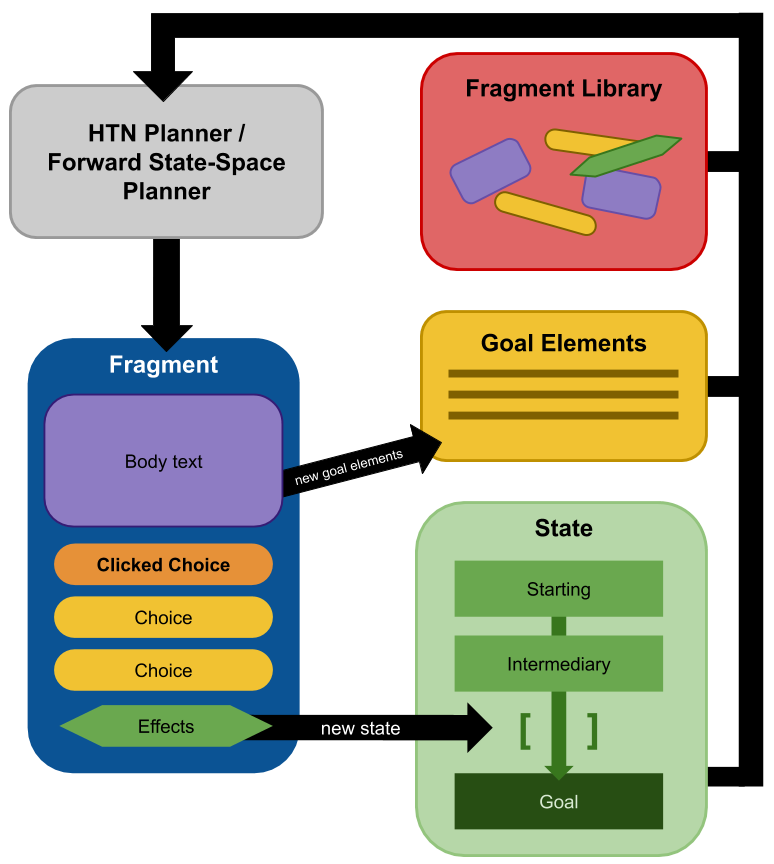
\includegraphics[width=\textwidth]{figures/3-StoryAssembler/storyassembler-system-diagram.png}
    \caption{A flow diagram of the StoryAssembler system.}
    \label{fig:system-diagram}
\end{figure}

\subsection{Core Architecture}
\label{core-architecture}

As mentioned earlier, StoryAssembler's core unit is the ``fragment", which is assembled from component parts in the ``fragment library." It chooses whatever valid combination best results in combined effects that modify the state blackboard to achieve (or make incremental progress towards) the goal state defined by the goal elements (Figure \ref{fig:system-diagram}).

It accomplishes this through two distinct components working in tandem: a forward state-space planner \cite{forwardPlanner} on the highest ``plot-progression" level, and an HTN-like planner  \cite{htn} used for the composition of fragments to accomplish that progression (Figure \ref{fig:htn}). Each StoryAssembler scene has a starting state with initial blackboard values of booleans, strings, or integers, and a goal state, composed of goal elements also represented as blackboard values, such as \texttt{introduceNemesis eq true}.

%%%%%%%% BEGIN FIGURE %%%%%%%%%%%%%%%%%%%%%%%%%%%%%%%%%

\begin{figure}
    \centering
    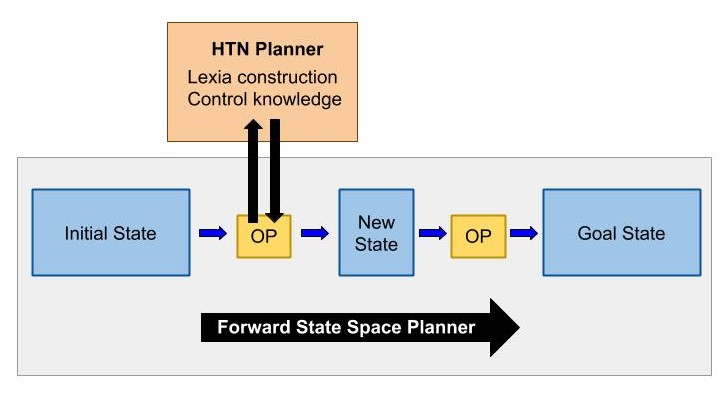
\includegraphics[width=\textwidth]{figures/3-StoryAssembler/htn-diagram.jpg}
    \caption{A simplified flow diagram of how the HTN planner and forward state space planner work together for fragment assembly.}
    \label{fig:htn}
\end{figure}

%%%%%%%%%%%% END FIGURE %%%%%%%%%%%%%%%%%%%%%%%%%%%%%%%%

When executed, StoryAssembler looks at the starting variables' states, looks at the goal state as a list of desired goal states, and then assembles fragments to push it closer to that goal. It does this by recursively searching the library for components---be that body text or choices---to maximize progress towards the goal state. Additionally, it scores fragments higher if they link to other fragments that make goal progress, or incorporate into themselves other fragments that make goal progress as compound fragments. In this way, the search is similar to one done by a hierarchical task network (HTN) planner, where each fragment in the library specifies a set of sub-tasks to pursue (e.g., finding choices or body-text with specific properties). The recursion / look-ahead depth for how many linking fragments are checked for scoring purposes is manually set. For example, in \textit{Emma's Journey}, we found that looking three ``choice-steps" ahead was more than enough to return sensibly-scored assemblages. Anything further may technically return ``better scoring results", but is at (or beyond) the limit of the design skills of authors, given the current tooling and available visualizations (which is discussed in \ref{clarity}).

The final assembled fragment represents the best next ``operation" for the forward state-space planner, and it continues in this manner until the scene ends. In short, StoryAssembler greedily optimizes for fragments that fulfill the maximum number of goal elements, as well as every choice in that fragment going to subsequent fragments that fulfill the maximum number of goal elements, et cetera. While larger questions of hill climbing and getting stuck in local maxima are valid, for us this implementation was sufficient to start tackling the \textit{authorial} concerns around expressiveness and authorial burden, so focus then shifted on how to produce content that could effectively leverage the strengths of this system.

Choice-based narratives are a particularly interesting and fruitful domain for planner-driven narrative systems, due to this additional combinatoric factor in the assembly of choices and displayed framing text. Because the framing text, the choice label, and the destination of the choice link are each their own atomic unit, it means those fragments can combine effects as compound operations, opening up a wide combinatoric space of possibilities. However, it's also these same compound combinatorics that come back to haunt us with challenges to Clarity when authoring content, which we'll expand on later in Section \ref{clarity}.

After the reader selects a choice, the system re-evaluates the current state, looks at the goal state, and re-plans to assemble the next fragment accordingly. Rather than pre-generating possible paths, this ``lazy evaluation'' was chosen because in its initial project (\textit{Emma's Journey}) a mini-game continuously runs in parallel, affecting StoryAssembler's blackboard state. Therefore, it made sense to not evaluate the path forward until the moment of the player's choice, in case an originally valid state was invalidated by gameplay while the text was displayed, or the reverse. 

Additionally, while StoryAssembler operates in this ``live'' mode, it can change displayed text and choices asynchronously in reaction to other game processes, or elapsed time, as detailed in Section \ref{templated-text}'s discussion of text templating.

%%%%%%%% BEGIN FIGURE %%%%%%%%%%%%%%%%%%%%%%%%%%%%%%%%%

\begin{figure}
    \centering
    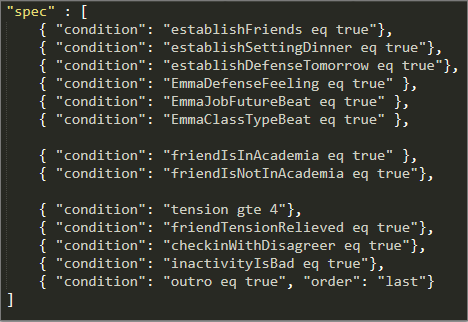
\includegraphics[width=\textwidth]{figures/3-StoryAssembler/story-spec.png}
    \caption{A sample goal state (``spec") detailing dramatic beats to be hit (boolean values) and mood conditions (tension).}
    \label{fig:story-spec}
\end{figure}

%%%%%%%%%%%% END FIGURE %%%%%%%%%%%%%%%%%%%%%%%%%%%%%%%%

\subsubsection{Goal States}

Each scene in StoryAssembler has a corresponding goal state containing a series of goal elements (Figure \ref{fig:story-spec}). A goal element, like blackboard entries, can contain boolean, string, or integer values, and authors may use them for anything from dramatic beats ({introduceFriend eq true}) to mood conditions ({tension gt 5}) or flags to inform the system where the reader has been, or which choices they've made ({complimentedWaiter eq true}). Goal elements can be partially ordered through possession of the optional tags ``first'' or ``last,'' but in general StoryAssembler treats them as an unordered list. The system will end the scene once every goal element has been satisfied at some point in the story (i.e., if a later fragment sets a boolean goal element such that it is invalid, it doesn't ``unsatisfy'' that entry). This design decision was made so that we could have more flexibility in the design of beats within a scene to change the underlying state to multiple values as the scene progressed. For example, if we wanted two characters to increase their \texttt{friendliness} stat after having an argument, we could put two goal elements \texttt{friendliness lt 2} and \texttt{friendliness gt 2} in our goal state. Of course, this also means authors must take care that reconciliation content that increases \texttt{friendliness} has pre-conditions of low \texttt{friendliness}, so that it doesn't prematurely trigger, but it was deemed an acceptable trade-off. This design decision also facilitated splitting up authoring tasks in scenes without reducing Clarity, because authors could focus on their allotted goal elements, and not necessarily worry about other goal elements that may not concern their narrative area.

Goal elements can also be flagged as persistent, which means the system will always prioritize content that satisfies them, but will not evaluate their satisfaction to gate whether the scene ends. This can be used to make the system prioritize repetitive actions, such as a professor calling on students during a lecture, or taking a turn in a conversation. Typically, this strategy is combined with explicit precondition design on fragments for repetitive actions, to control ordering.

A good example of how goal elements work is the first scene of \textit{Emma's Journey}: the night Emma dines with friends before her PhD defense. This scene's goal state (Figure \ref{fig:story-spec}) contains key elements that both communicate setting ({establishFriends eq true}) and initiate the narrative dynamics. The goal state requires two characters to make their cases whether Emma should pursue academia or activism, that the tension in the room passes a certain threshold (via fragments that increment a \texttt{roomTension} variable), and that Emma discusses her own career aspirations. A library of fragments have been authored that can achieve these goal elements in a variety of configurations, which are assembled by the system into a choice-based narrative, and re-shuffled around depending on how the player makes their choices.

\paragraph{Dynamic Goal States}
\label{dynamic-story-specs}

An interesting advanced authoring capability with StoryAssembler is the ability to make goal elements dynamic. This enables techniques such as exposing them to the player as ``scene settings" before the story starts (Figure \ref{fig:parameterized-summary}). For \textit{Emma's Journey}, we implemented this as ``cycling links'' in the scene description. Players can click on the links to change their text values, which in turn affect the goal elements, and the way the scene plays out once they begin. For example, if the player decides to have both friends more critical, the resulting story the planner assembles will have them challenging the player more on their career choices.

%%%%%%%% BEGIN FIGURE %%%%%%%%%%%%%%%%%%%%%%%%%%%%%%%%%

\begin{figure}
    \centering
    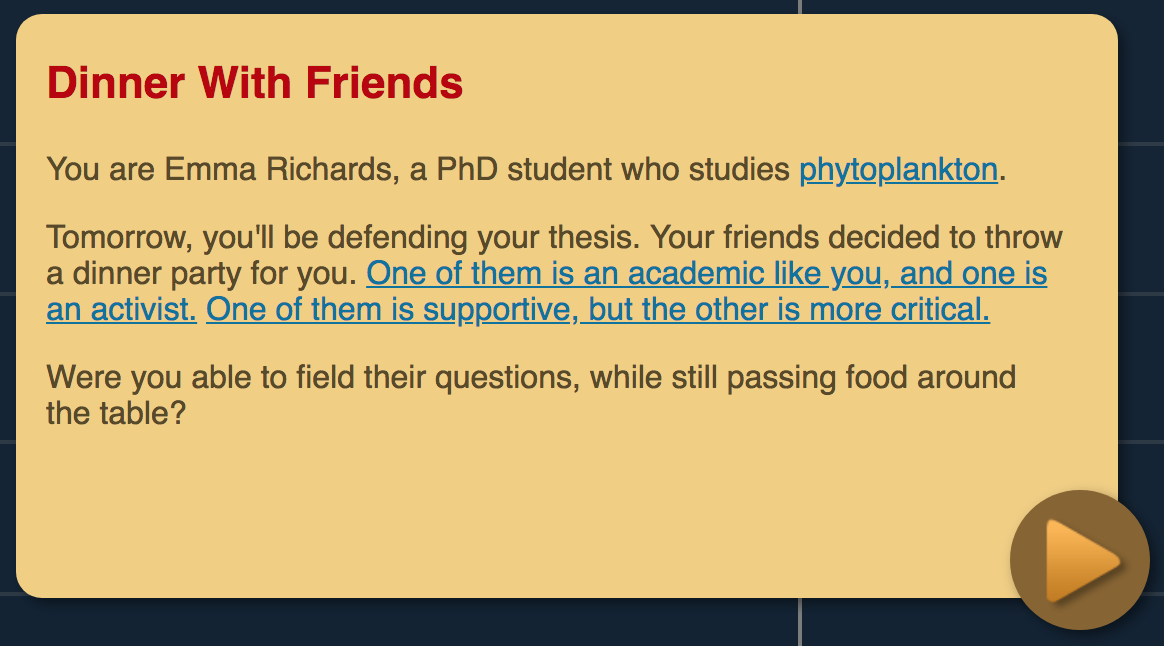
\includegraphics[width=\textwidth]{figures/3-StoryAssembler/parameterized-summary.png}
    \caption{A scene intro, where dynamic goal elements allow players to change friends to be activists or academics, and supportive or critical, as well as Emma's research focus.}
    \label{fig:parameterized-summary}
\end{figure}

%%%%%%%%%%%% END FIGURE %%%%%%%%%%%%%%%%%%%%%%%%%%%%%%%%

In earlier prototypes, this was alternatively exposed as a literal control panel, allowing players to drag sliders around and toggle options on or off. One can imagine this giving rise to several interesting modalities for experiences, and perhaps such controls could even be incorporated into the narrative of the game itself, making them a diegetic way to both surface the capabilities of the system, and deepen the player's engagement.

\subsubsection{Fragment Libraries}

For each scene in StoryAssembler, JSON files of fragments are specified for use. The ability to specify multiple files became a particular asset due to the team-based authoring, as it allowed writers to each use their own file, and substitute placeholder fragments handling other goal elements that other writers were working on. This allowed us to easily develop the game with a sort of rough version control without having to negotiate typical problems with on-boarding such as negotiating merge conflicts, which can be confusing to writers unfamiliar with such systems.

In terms of narrative design pragmatics, this also makes it possible to organize fragment libraries by other features, such as tone, character, or chronology. Or, as in early prototypes of \textit{Emma's Journey}, specify a global library of fragments with highly dynamic, condition-driven text, that could potentially appear within any scene in the narrative. This type of flexibility is similar to what was done in \textit{Ice-Bound} with the level-specific card files, and the global symbol cards file.

\subsubsection{Fragments}

StoryAssembler's core unit of narrative is the fragment. In their canonical form, fragments contain a main section of displayed text (``content"), and a list of choices (``choices"). This is similar to the basic ``passage'' in Twine.

Fragments can also contain pre-conditions to control when they're available. Design-wise, these can be used for causal or temporal ordering. Lastly (and most importantly) fragments can contain effects, which change the state blackboard. This is what is evaluated to determine if the assembled fragment makes progress towards the goal state specified in the scene configuration, and thus drives where and when a fragment will appear. These state modifications can optionally carry through between scenes if authors desire, allowing certain choices to affect later points of the narrative. An example of a fragment data structure can be seen in Figure \ref{fig:sample-fragment}.

%%%%%%%% BEGIN FIGURE %%%%%%%%%%%%%%%%%%%%%%%%%%%%%%%%%

\begin{figure}
    \centering
    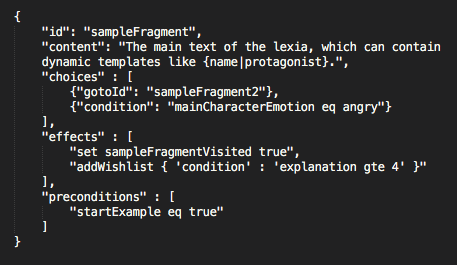
\includegraphics[width=\textwidth]{figures/3-StoryAssembler/sample-fragment.png}
    \caption{A sample fragment showing both static choices (``gotoId") and dynamic choices (``condition") as well as modifying goal elements through effects (``addWishlist").}
    \label{fig:sample-fragment}
\end{figure}

%%%%%%%%%%%% END FIGURE %%%%%%%%%%%%%%%%%%%%%%%%%%%%%%%%

A key capability driving the authorial affordances of StoryAssembler is that fragments can be \textit{compound}, or composed of other fragments. For example, a fragment might contain ``normal" choices (static choice text that directs to another node directly by id) but in place of ``content'' (the main text of the fragment) might instead contain a ``request'' for any valid fragment that increments tension. StoryAssembler then looks for a valid fragment that 

\begin{enumerate}
    \item has effects that increment tension (such as ``tension incr 1")
    \item has a ``content" field with text, but doesn't have choices (ie, it was authored not to stand alone, but to be part of a compound fragment)
\end{enumerate}


It then takes the value in that new fragment's content field, and any effects it has, and combines that with the previous one. The resulting compound fragment would trigger the effects for both of the partial fragments, and would have the body text from the second fragment, with the choices from the first.

Another useful way to think about this is that an assembled fragment in StoryAssembler has three components, each of which uses one of three methods. 

The fragment components are:

\begin{enumerate}
    \item One block of text for ``main content"
    \item A short piece of text for each choice (the ``choice label")
    \item A reference to another assembled fragment visited when the player clicks each choice
\end{enumerate}

Similarly, there are three modes these components can operate in:

\begin{enumerate}
    \item A fragment component can be a non-referential ``string", such as the ``content" field in the Figure \ref{fig:sample-fragment} fragment, which does not reference any other fragment. A fragment can have a string for content and choice label, but a string cannot be used for the choice destination (since by definition it must reference the destination fragment).
    \item A fragment component can be an ``id", which directly links to another specific fragment by its unique id. The first choice in the ``choices" array in Figure \ref{fig:sample-fragment} links to ``sampleFragment2" by id using the ``gotoId" command. All three fragment components can use this mode.
    \item A fragment component can be a ``request", which triggers a search for the most suitable fragment that meets the conditions of the request. The second choice in Figure \ref{fig:sample-fragment} requests any fragment that has an effect setting "mainCharacterEmotion" to ``angry." All three components can use this mode.
\end{enumerate}

Additionally, identical state condition requests can be used for multiple choice destinations, and the system will choose different ``assemblages" to satisfy them, ensuring each choice path is different. For example, one could write a fragment with three choices, two of which increase the tension in the room, and one that alleviates it. StoryAssembler will search the fragment library for unique choice paths that lead to those state changes, and link them in. This enables potentially surprising juxtapositions of paths, and emergent traversals driven by underlying state changes and tracked stats.

While these might seem relatively simple in definition, in practice they can become quite complex, and enable different kinds of narrative experiences. A chart of the different formulations can be seen in Figure \ref{fig:fragment-table}, although many of those remain speculative, given that \textit{Emma's Journey} relied mostly on a handful of formulations, as detailed in Section \ref{implementation-details}'s discussion.

%%%%%%%% BEGIN FIGURE %%%%%%%%%%%%%%%%%%%%%%%%%%%%%%%%%

\begin{figure}
    \centering
    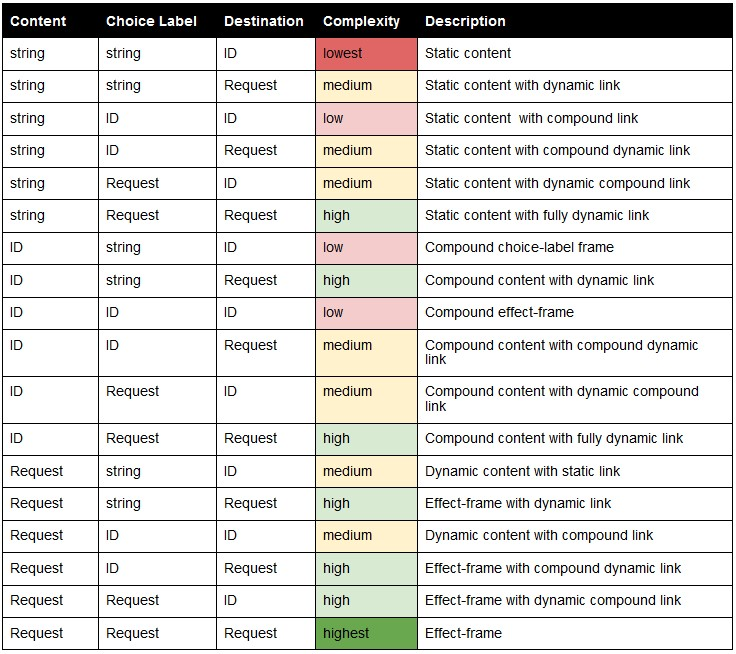
\includegraphics[width=\textwidth]{figures/3-StoryAssembler/fragment-table.jpg}
    \caption{A table of the different StoryAssembler fragment combination methods. Some have somewhat similar affordances (such as ``static content" and ``static content with compound link") and some are quite different. We use ``effect-frame" to designate combinations where the fragment's purpose is to provide a ``frame" for other fragments to be combined within. It has little to no content of its own, but its purpose is a specific content juxtaposition, or addition of its effects to other fragments.}
    \label{fig:fragment-table}
\end{figure}

%%%%%%%%%%%% END FIGURE %%%%%%%%%%%%%%%%%%%%%%%%%%%%%%%%

At the other end of the complexity scale, fragments don't always have to link to other fragments. If no choices are specified in the fragment, the system finds the next best fragment (with valid preconditions) that satisfies the most remaining goal elements, and links to it by creating a ``Continue'' choice. This method frees up authors to author dramatic ``beat'' structures that have internal consistency, but are independently ordered.

In short, StoryAssembler's process is to construct fragments, then evaluate recursively through the choices afforded by the fragment, choosing paths that maximize state changes to fulfill goal elements. In general terms, this means StoryAssembler is always greedily assembling fragments that both contain as many goal-oriented effects as possible, and linking to the most goal-oriented fragments possible. A fragment's effects, choices, and preconditions therefore all play into that process, and must be kept in mind while authoring.

As mentioned before, StoryAssembler can also operate in a ``live'' mode, where at a given interval it re-evaluates the displayed text and choices. If the state has somehow changed while the player was reading the fragment (through an accompanying game mechanic, as with \textit{Emma's Journey}) choices can become unavailable and grayed out, or similarly become available. This affordance can be used to inject urgency into player actions, or make procedurally poignant effects. For example, in a tense conversation with the dean, Emma might lose access to choices to steer the conversation where she wants, if the player's performance in the accompanying mini-game is lackluster. This affordance was added with early Twine works in mind like \textit{Depression Quest} \cite{quinn_2013}, which used the visibility--yet unavailability--of choices as a communicative and persuasive strategy.

\subsubsection{Templated Text}
\label{templated-text}

StoryAssembler's text templates were designed to have similar capabilities to \textit{Ice-Bound}'s. Templates can be used to change the presentation of both fragment content and choice labels. This can be driven by scene state---for example, authors can add hedges like ``umm...'' to dialogue if the state variable ``confidence'' falls below a threshold. This is especially useful when used in tandem with live state modification, as with \textit{Emma's Journey}, where it can signal time-sensitivity to the player, or otherwise communicate the narrative consequences of mini-game performance.

We can also change content more substantially, so that fragments change under different state contexts. For example, we may decide to create a fragment ``complimentHost'' where Emma compliments the host's decor if dinner hasn't started yet, but compliments the food if that fragment is triggered when \texttt{dinnerStarted eq true}. In either case, the fragment's effect to decrease tension is fired, but the text surfacing that is contextual to the current situation.

Templates can also reference character names, pronouns, and other individual mix-ins, so that fragments can be written that are not tied to a specific scene, but rather globally mixed into scenes if their pre-conditions are valid. 

Templates can also be leveraged outside of fragments to have more structural impact. For example, templates can be used in a scene's ``config file", giving authors the ability to cast characters for scenes dynamically, or choose different character qualities before the scene starts that have a perceivable effect on the story. For example, a challenging character can be authored simply as ``antagonist'' and in a previous scene, set as whoever the player escalates a disagreement with. This is gone over in more detail in Section \ref{complexity}'s discussion of Complexity.

\subsection{Emma's Journey}

StoryAssembler was implemented as a JavaScript library. This decision was made due to a couple different factors. One, coming on the heels of \textit{Ice-Bound} (which was entirely built in JavaScript) there was a high degree of comfort with it as a language (the dynamic templating language could be almost directly adapted, functionally speaking). Additionally, the main project driving its development--Emma's Journey--had another component (Gemini) which output Javascript mini-games. The requirement that these two systems talk to each other, and at times modify the state of each other, meant that a common language would be best. While certainly it would be possible to re-implement or ``port" StoryAssembler to another language, its base implementation and feature set was driven mostly through the pragmatics of the project detailed below.

\subsubsection{Implementation Details}
\label{implementation-details}

\textit{Emma’s Journey} is an experimental narrative game that juxtaposes a choice-driven narrative (implemented as a series of StoryAssembler scenes) with a succession of abstract mini-games generated by the Gemini system \cite{Gemini}. It served as a testbed for the development of StoryAssembler and is the first experimental research game to make use of the system \cite{emmaWorkshop}. 

As mentioned in Section \ref{experience-challenge}, the side-by-side presentation of the narrative and generated games is reminiscent of Molleindustria’s ``two-channel narrative game" \textit{Unmanned} \cite{Unmanned}. Players experience a series of scenes from the life of the titular character Emma, initially a climate researcher preparing to defend her PhD dissertation, and make choices that influence the progression of Emma’s career while the world’s climate changes in the background. 

In each scene the player is presented with a single generated mini-game, which interacts with the narrative. We experimented with several different modalities in this project: 

\begin{itemize}
    \item losing the mini-game resulting in a fragment jump in the narrative to a ``losing" path that quickly ends the story
    \item using text templates to change sentences on a word-by-word level progressively as performance worsens in the game for a maintenance task
    \item conditioning choice availability based on game state, making certain choices only available if game performance is good (reminiscent of Quinn’s \textit{Depression Quest} \cite{DepressionQuest})
    \item locking narrative progression to game progression (with no loss condition for the game)
\end{itemize}

In one scene, for instance, Emma is eating dinner with her friends, and the player must play the mini-game to pass food around the table (Figure \ref{fig:gemini-game}). Failure to do so with sufficient frequency will result in the game interrupting the narrative, blocking progression until the player passes the food again. 

In a scene using the ``progression lock", the player must play the mini-game to clean up a beach while holding a conversation with fellow volunteers. The progression of the conversation stops with a ``let's clean up some more" until a checkpoint is passed, which then unlocks the choice to continue. In one of the more difficult scenes, the mini-game performance controls Emma’s concentration during a lecture in front of her class. As the player's performance deteriorates, awkward hedges start appearing in Emma's lecture, ultimately resulting in a narrative failure that ends the scene prematurely if the game is lost. A subsequent scene with the Dean showcases many of these dynamics in unison, as detailed in the following section.

%%%%%%%% BEGIN FIGURE %%%%%%%%%%%%%%%%%%%%%%%%%%%%%%%%%

\begin{figure}
    \centering
    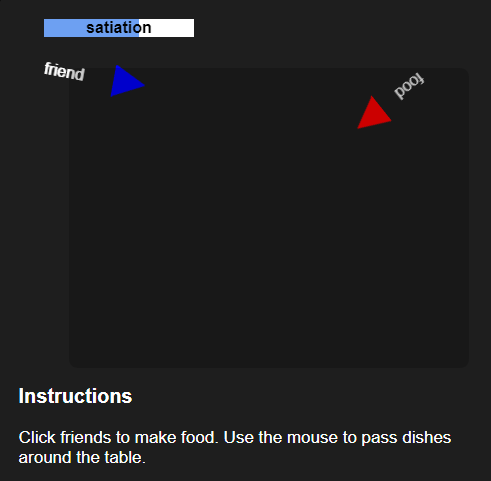
\includegraphics[width=10cm]{figures/3-StoryAssembler/game.png}
    \caption{A Gemini-generated minigame. In this case, the game revolves around passing food around a table.}
    \label{fig:gemini-game}
\end{figure}

%%%%%%%%%%%% END FIGURE %%%%%%%%%%%%%%%%%%%%%%%%%%%%%%%%

Gemini, the system responsible for generating the mini-games that accompany each scene's narrative, is a game generation tool based on what Treanor et al. term proceduralist readings \cite{treanorProceduralistReadings}: interpretations of a game’s ``dynamics, aesthetics, and higher-level meanings" deduced directly from its mechanics, in conjunction with a corpus of cultural knowledge. Gemini accepts as input a file of desired ``readings" or interpretations for the generated game, specified in the form of a logic program, and uses answer set programming to work backwards from these specifications and construct games that can be read in the desired ways. These mini-games have a couple variables that broadcast their values to StoryAssembler, which can then change the displayed fragment, or fragment text, accordingly.

And indeed, some of the most poignant affordances can result from this: a mini-game which requires constant attention as the reader watches Emma’s narration grow increasingly nervous, or confident action choices graying out as the player’s performance in the game lags behind. The trade-off is that StoryAssembler must re-plan at each reader choice, since the mini-game may change the state in the interim before the next click, such that those pathway destinations are no longer optimal or even valid. 

The plot structure of \textit{Emma's Journey} went through many iterations before its release. The scene which showed off the widest array of the system's capabilities in these iterations, however, remained the ``Dean's Office" scene, which occurred third in the final sequence.

\paragraph{Dean's Office}

The Dean's Office scene was third in the progression--after the player had taken Emma through a dinner with her friends, and her first lecture with her students. The player established both her area of expertise and her class dynamics through use of the cycling links that modified the goal state for each respective scene, and were surfaced in fragments during the meeting with the Dean.

%%%%%%%% BEGIN FIGURE %%%%%%%%%%%%%%%%%%%%%%%%%%%%%%%%%

\begin{figure}
    \centering
    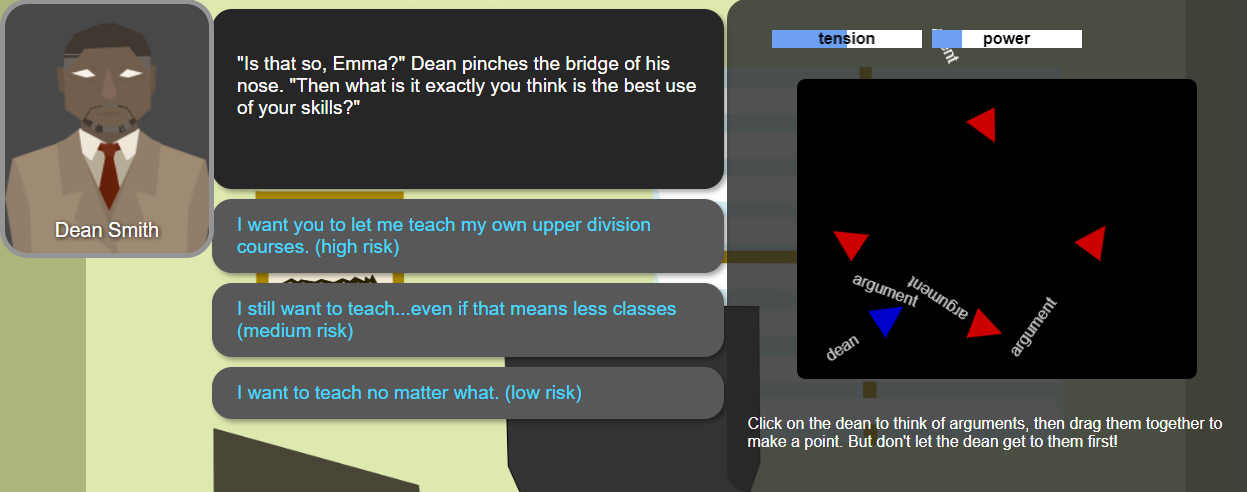
\includegraphics[width=\textwidth]{figures/3-StoryAssembler/dean-level.png}
    \caption{The Dean's Office scene. Here we see the mini-game on the right, which increases power if the player performs well. The choices on the left are labeled ``high risk" to ``low risk." When clicked, they increase the tension, which modifies the game difficulty. Subsequent choices are gated off power values, so poor performance results in not being able to make choices for a good outcome to the scene.}
    \label{fig:deans_office}
\end{figure}

%%%%%%%%%%%% END FIGURE %%%%%%%%%%%%%%%%%%%%%%%%%%%%%%%%

The main dynamic architecture of this scene revolves around whether Emma has succeeded or failed in the previous lecture scene. The lecture scene featured a mini-game that the player could lose, if they weren't performing the maintenance task. Combined with the cognitive overhead of reading a story and making choices, it was easily the most difficult section of the game. If the player had succeeded in the lecture, the Dean would try to pressure them to take on more classes. If they had failed, they would need to justify why they shouldn't be fired.

The Dean's Office has two main variables being tracked: \textit{tension} and \textit{power}. \textit{Tension} relates to whether the scene can finish out to completion (if tension is too high, the scene ends prematurely) and also the difficulty of the mini-game. \textit{Power} is how assertive Emma can be during the conversation to get what she wants (if power is low, conversation options are grayed out and unclickable).

The player can make choices that increase the tension, such as requesting a pay raise or better working conditions. However, if their performance in the game hasn't raised their power enough, when it comes to the choices for giving reasons to justify the requests, they'll be grayed out, forcing the player to capitulate. These values are modified as the game is playing, so may change second-to-second.

Lastly, The Dean’s Office demonstrates on a macro level how scenes can branch based off of conditions in previous scenes. Depending on which ending occurs here, the next scene is dynamically chosen to be either one in which Emma gives a presentation at the UN on climate change for a more ``global effect", or one in which she helps a local non-academic organization relocate an endangered crab species to a new location, for a more ``local effect."

This scene flexed many of the StoryAssembler's interfacing capabilities, and showed how one scene can both have different ways it plays out due to context from previous choices, and can also lead to different subsequent scenes based on the player's choices and performance within that scene.


\subsubsection{Additional Capabilities}

Some capabilities of StoryAssembler were developed, then disabled later on as \textit{Emma's Journey} neared completion. These cuts were made due to pragmatic reasons--sometimes due to difficulties they introduced in content design, sometimes due to feedback from UI usability--but are still interesting to highlight from a system capability standpoint, and as a point of reference for people pursuing similar capabilities.

\paragraph{Global Fragments}
\label{sa-global-fragments}

Initially, we wanted to have a library of global fragments that could be used in multiple contexts within different scenes. It was thought that, if appropriately authored, this could reduce authorial overhead through contextual reuse, without the story seeming to repeat itself. However, in practice it became difficult enough to author fragments that wouldn't seem out of place, that the work involved became greater than if more numerous, specific fragments had been written. As a result, this approach wasn't pursued for \textit{Emma's Journey}. However, the use of multiple content libraries for an individual scene was used to enable multiple authors to work in parallel on the scene, so this capability still exists, just not in the design of \textit{Emma's Journey}. This is elaborated upon in Section \ref{sa-reusability}'s discussion of Reusability.

\paragraph{Dialogue Mode}

For a time we experimented with using a ``dialogue mode" for scenes, which could be set to ``monologue" or ``dialogue" (Figure \ref{fig:discourse-data}). This was then used as an additional scoring heuristic for fragment selection, in the attempt to prioritize fragments that had the correct speaker. This in turn predicated us adding a new field of ``speaker" to every fragment. These values could be statically set to be specific characters, or dynamically determined based on character tags or traits. Speaker fields would be resolved at the beginning of each scene. It was hoped that, since it would position fragments with primary speakers, we could then lean into templated ``mixins" to give them more individual flavor, and add more replayability. It was hoped that if a scene were replayed with different characters cast into different roles, it would feel substantially different, even if the ``bones" of the scene remained the same.

%%%%%%%% BEGIN FIGURE %%%%%%%%%%%%%%%%%%%%%%%%%%%%%%%%%

\begin{figure}
    \centering
    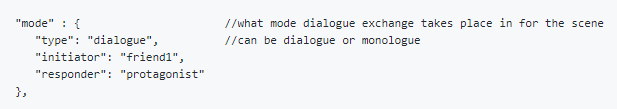
\includegraphics[width=\textwidth]{figures/3-StoryAssembler/data-object-2.png}
    \caption{Data object for discourse mode, here set to ``dialogue" with the character cast as ``friend1" starting off the scene, and the ``protagonist" responding.}
    \label{fig:discourse-data}
\end{figure}

%%%%%%%%%%%% END FIGURE %%%%%%%%%%%%%%%%%%%%%%%%%%%%%%%%

This was simplified out of the library, because after many drafts of content in \textit{Emma's Journey}, it was determined the complexity overhead it added to authoring (See Section \ref{complexity}) wasn't worth the small amount we were leveraging for the story. Additionally, on a narrative design level, it would require adding meaningful differences or changes to the scene story depending on different speakers, and it was hard enough keeping within scope with a static number of characters.

\paragraph{Avatars and Exposed Character Stats}

We did end up using the ``assigned speaker per fragment" design for providing an avatar for whichever character was speaking. These weren't just static images--different avatars for character emotions were created, and then set with value boundaries tied to different state variables. For example, if Emma's confidence falls below a certain threshold while giving a lecture, her avatar changes from a smiling one to a more worried one. The purpose was to provide another avenue to surface the blackboard values to the player (in addition to what was going on with the mini-game) and increase the feeling that the game was reactive and ``listening" to them.

While only one character is shown per fragment in the final version of the game, in early drafts the salient characters for a scene would be shown at the bottom of the screen in a manner reminiscent of RPG characters. Rather than simply binding variable thresholds to control which avatars were shown, multiple values could be bound to single or multiple characters, which would display as ``stat bars" (Figure \ref{fig:lecture}).

%%%%%%%% BEGIN FIGURE %%%%%%%%%%%%%%%%%%%%%%%%%%%%%%%%%

\begin{figure}
    \centering
    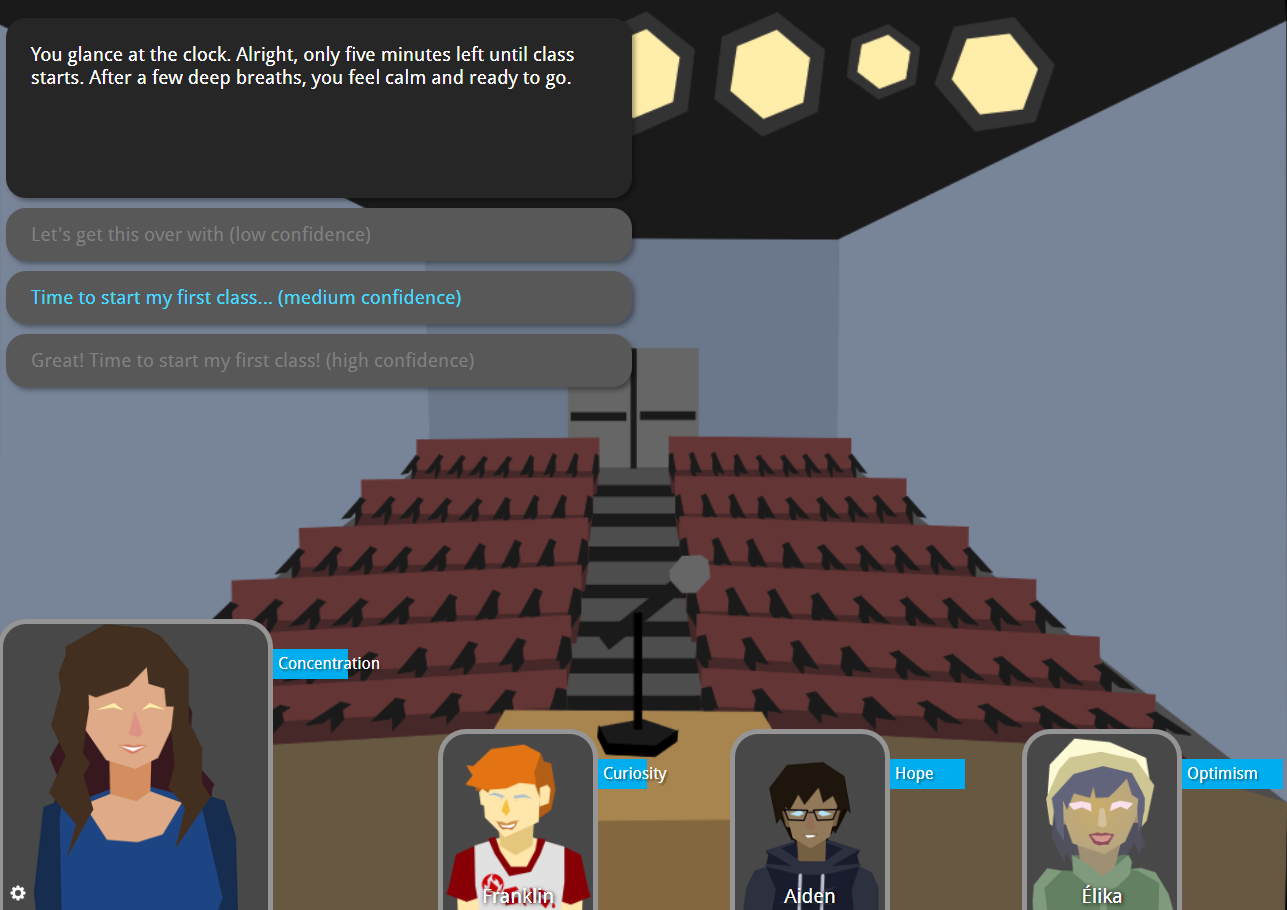
\includegraphics[width=12cm]{figures/3-StoryAssembler/lecture.png}
    \caption{An early prototype, showing state variables bound to characters as ``stat bars" that updated as their values changed.}
    \label{fig:lecture}
\end{figure}

%%%%%%%%%%%% END FIGURE %%%%%%%%%%%%%%%%%%%%%%%%%%%%%%%%

As choices were made with the narrative, players could immediately see how certain choices would change values for other characters, such as ``curiosity", ``hope", or ``optimism." It was hoped that this would help drive home that the choices the player was making were having an effect on the state of the game. After some focused testing with players, however, it was found that the stat bars--when seen in concert with the also-changing mini-game bars--created an information overload, which decreased their utility. Therefore, we made the design decision to only reflect macro-changes through avatar state changes, and keep the mini-game stat bars as the only surfaced qualities the player sees. This made sense for \textit{Emma's Journey}, as most of the scenes where the values were important information were scenes in which the mini-game was the main method used to modify them. However, for possible future games using StoryAssembler, the use of stat bars with characters may prove a useful capability.

\paragraph{Scene Selection UI}

For \textit{Emma's Journey}, two different UIs were developed for scene selection. The first was a scene selection list, where each story scene was placed in a column incrementing through the years (Figure \ref{fig:scene-ui-proto}).

%%%%%%%% BEGIN FIGURE %%%%%%%%%%%%%%%%%%%%%%%%%%%%%%%%%

\begin{figure}
    \centering
    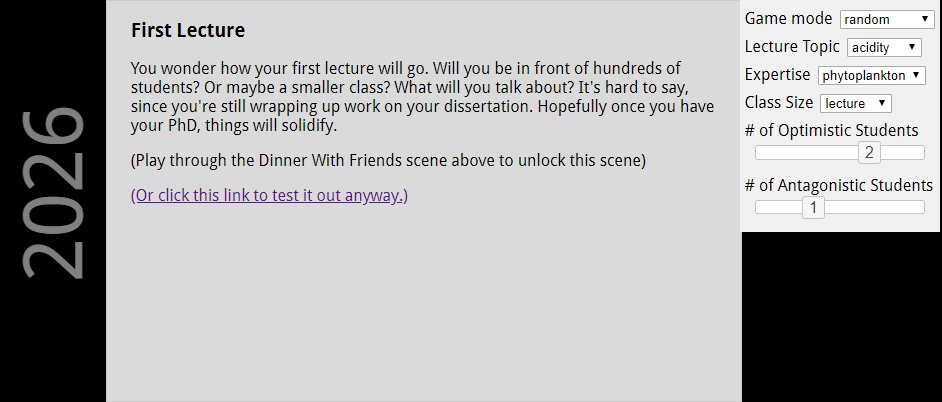
\includegraphics[width=\textwidth]{figures/3-StoryAssembler/proto-UI.png}
    \caption{The ``scene selection" UI layout. Notice the panel to the right. Changing the values here changed parameterized goal elements, driving different priorities for the planner once the scene was begun. This was a less diegetic way of achieving the same effect later realized through cycling links in short scene descriptions.}
    \label{fig:scene-ui-proto}
\end{figure}

%%%%%%%%%%%% END FIGURE %%%%%%%%%%%%%%%%%%%%%%%%%%%%%%%%

When the player clicked the scene, a pop-out control panel on the right would let them set individual scene parameters, which were then sent to the system as modified goal elements. Because the goal state would be different, players could force the system into different formulations for the scene. 

We also experimented with players being able to start a scene at any point in the story timeline, even the last scene first if they wanted! However, the paradoxes of players experiencing scenes out of order, yet wanting to have consequences from earlier scenes affect scenes later in time, meant that we needed to move to a more temporally restricted interface. We attempted having ``bindings" between scene variables, such that players could change variables in temporally earlier scenes to effect later scenes, but in the end it was determined it was too complex an interface for the dynamisms it represented, and we went with a more streamlined appearance.

%%%%%%%% BEGIN FIGURE %%%%%%%%%%%%%%%%%%%%%%%%%%%%%%%%%

\begin{figure}
    \centering
    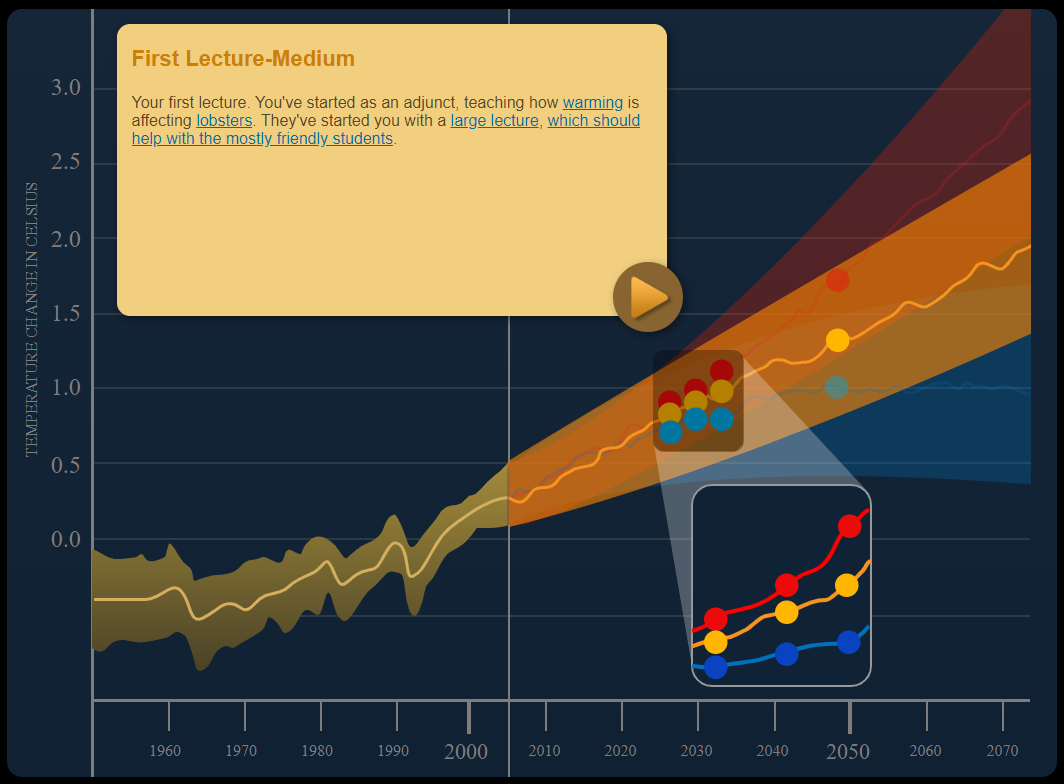
\includegraphics[width=12cm]{figures/3-StoryAssembler/scene-ui.png}
    \caption{Timeline interface for \textit{Emma's Journey}.}
    \label{fig:scene-ui}
\end{figure}

%%%%%%%%%%%% END FIGURE %%%%%%%%%%%%%%%%%%%%%%%%%%%%%%%%

The final interface for \textit{Emma's Journey} was a timeline of the three climate change curves from the \textit{IPCC Report} \cite{ipcc}. The low blue curve represents action taken such that emissions tail off (referred to as the RCP 2.6 curve). The medium yellow curve (RCP 4.5) is if only some action is taken, and the high red curve (RCP 8.5) is if little to no action is taken. At the beginning, the player chooses which line they want to play out. This sets a particular variable for the scenes, which changes some subtle things in the way it is realized. Play then continues scene-by-scene. 

As mentioned earlier, each ``dot" on the timeline has a pop-up paragraph of text with cycling links, which change to new values when clicked. This way, the player can still influence the parameters of the scene, but in a more diegetic way, compared to the previous control panel. Additionally, constraining it to only be traversable in temporal order meant we could side-step potentially confusing the player before they even started playing.

This interface of navigating through a game by traversing a graph is one that has been used in other games as well to emphasize and showcase the choice-driven nature of their narrative, and allow the player to properly appreciate how their decisions scene-to-scene are mapping to the overarching story. For example, the game studio Chunsoft's \textit{Zero Escape} (2012) and its sequel \textit{Zero Time Dilemma} (2016) both prominently feature an interactive flowchart for narrative navigation, allowing the players to choose which scene they play next, or whether they want to replay an earlier segment to get different outcomes and options \cite{mackey_2016}. A screenshot of the ``global flowchart" can be seen in Figure \ref{fig:ref-plot-diagram}. The interplay in that game series between mini-game and narrative is also similar to \textit{Emma's Journey}, in that scenes are predominantly story-based (similar to a visual novel) or game-based (where players have to complete skill-based challenges). Later works like Quantic Dream's \textit{Detroit: Become Human} \cite{dream2016detroit} and Netflix's \textit{Bandersnatch} \cite{bandersnatch} also use this strategy, perhaps as well to show that despite the filmic qualities of the media (that one might then associate with linearity) there are many different paths to the experience, in the hope of foregrounding replayability.

%%%%%%%% BEGIN FIGURE %%%%%%%%%%%%%%%%%%%%%%%%%%%%%%%%%

\begin{figure}
    \centering
    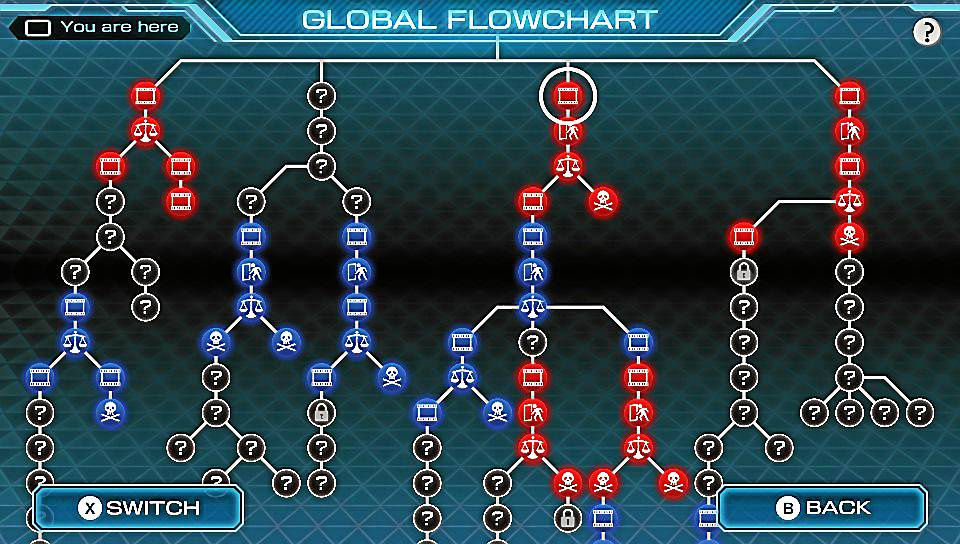
\includegraphics[width=\textwidth]{figures/3-StoryAssembler/ref-plot-diagram.png}
    \caption{Screenshot of the scene selection interface in Zero Time Dilemma.}
    \label{fig:ref-plot-diagram}
\end{figure}

%%%%%%%%%%%% END FIGURE %%%%%%%%%%%%%%%%%%%%%%%%%%%%%%%%

Other games, like \textit{Radiant Historia}, incorporate timeline views as diegetic elements of their story the player accesses and traverses, in this case enabled by a magical book that lets them explore ``Time Nodes" \cite{radiant_historia}. Regardless of diegetic situatedness, this concept of ``exploring different timelines" was something we wanted to employ for \textit{Emma's Journey}, to encourage the player to try different RCP curves and see how the future--and Emma's options--differed.

\section{The Question of Authorial Leverage}

In contrast to \textit{Ice-Bound}, the development of StoryAssembler (and through it, \textit{Emma's Journey}) was much more focused on the development and exploration of new dynamic choice-driven narrative capabilities than the telling of a particular story. For \textit{Ice-Bound}, much of the story was developed up front, and once we had a system capable of telling that story, development of additional system features largely stopped. For StoryAssembler, the exploration of new territory and capabilities was the priority, and we would then see what sort of stories were enabled by them. As such, the story scope and system were under more flux as capabilities were explored, authoring was attempted with them, and they were either reinforced or discarded as infeasible for content production, given the parameters of the project. 

Because of this, \textit{Emma's Journey} has a wide range of Traversability taken across its prototypes, and Authorability for those differed based on efforts made to mitigate the increase in state space and complexity. We will dive into these different states of the project, what we did to try to manage the complexity, culminating in some lessons learned and authoring patterns used along the way.

\subsection{Traversability}

\subsubsection{Explorability}

The entire motivating premise of StoryAssembler revolves around the idea that the content can be dynamically assembled, thus used in a variety of contexts, thus increasing authorial leverage. Ideally therefore, something in the neighborhood of 75\% of authored fragments should be used within a given playthrough of the game, consisting of a complete path through the scenes. In subsequent playthroughs, many of the same fragments might be re-visited, but some different scenes may be triggered due to state differences, driven in part by the state dependency on the mini-game, resulting in a very different outcome.

%%%%%%%% BEGIN FIGURE %%%%%%%%%%%%%%%%%%%%%%%%%%%%%%%%%

\begin{figure}
    \centering
    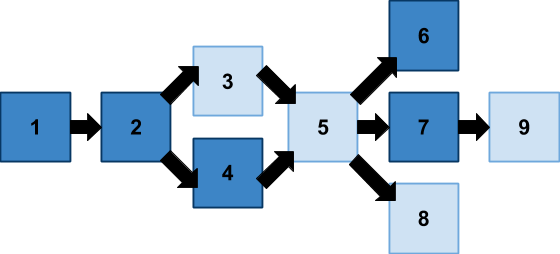
\includegraphics[width=\textwidth]{figures/3-StoryAssembler/plot-diagram.png}
    \caption{A scene-flow diagram for \textit{Emma's Journey}. Light blue squares denote scenes that existed in earlier drafts, but were cut for the final version.}
    \label{fig:plot-diagram}
\end{figure}

%%%%%%%%%%%% END FIGURE %%%%%%%%%%%%%%%%%%%%%%%%%%%%%%%%

Figure \ref{fig:plot-diagram} shows a scene-flow diagram for the intended experience, with lighter squares being ones which unfortunately had to be cut due to time constraints, though they existed as completed StoryAssembler scenes and could be played through in earlier drafts. The goal was to provide both individual variability on the level of the ``choice-trees" constructed in each scene, and from the performance and choices in those scenes, determine which scene would come next.

In terms of how large a state space the narrative is responsive to, \textit{Emma's Journey} was designed with a few key variables for each scene that would vary by a certain amount. When planning out each scene in narrative design meetings, we would make a list of the variables that affected the narrative, the game, and both, and enumerate their dynamics. For example, in Scene 1 (the dinner scene) we track ``confidence", ``enthusiasm for academia", ``tension", and the two friend relationships. Higher confidence opens up more options for Emma to diffuse tension when her friends argue, and her enthusiasm for academia determines which friend dominates the exchange. The tension variable, which rises as the friends disagree, increased the difficulty of the game (in earlier drafts). Enumerating these dynamics early on became critical as authoring progressed for the game, because once the individual fragments were being authored, it would be easy to lose sight of the scene-wide dynamics we were hoping to achieve.

Those were the specific considerations for \textit{Emma's Journey}. In terms of general capability, however, StoryAssembler's state space is left unformalized to the point of being a simple dictionary. Thus, there are no system-imposed limitations on how large a state space stories in StoryAssembler can have. In works like \textit{Emma's Journey}, where it was placed in dialogue with a mini game, the state space could be rather fine-grained (for some levels, we would track multiple values of variables between 0 to 10, whose combinatorics quickly raise that number). However, due to authoring pragmatics, we would ``bin" these values between ranges, and those ranges would typically be simple thresholds to binaries, or three-bin states. Additionally, taking an aforementioned page from Failbetter's book, we tried to hew closely to ``quality parsimony," and use as few variables as possible for these dynamics, in order to make it easier to track state when authoring.

In summary, the types of narrative design StoryAssembler supports and enhances are geared towards context-sensitive and adaptive content, through both the pre-condition logic, and the state-dependent templating that can rework the surface-level text of fragments to preserve coherency if displayed in different situations. Therefore, by implication, the types of games it enables should lean from medium to high explorability, in order to leverage these strengths.

\subsubsection{Replayability}

For \textit{Emma's Journey}, it was hoped that the player might play through multiple times, to experience the difference of the three climate timelines, or make different choices in the scenes. After all, even if interesting choices exist, players may also wonder about branches they haven't explored, which could potentially set us up with issues of repetition for replayability. However, the main focus was on variability and reactivity within the fragments themselves, with a couple hooks present to change which scenes would be activated next. The design implications of this were that we needed to surface the dynamism of the system to the player as we went, as we wouldn't rely on subsequent playthroughs or going back to a previous scene to showcase the variance of fragments. Because the partnered mini-game interaction provided a way to modify the fragments live, this was something we could lean into, as opposed to hoping a subsequent playthrough might get the player into a different situation. However, that still set us up with a requirement of medium to low Replayability, specific to \textit{Emma's Journey}. This de-prioritization is in contrast to \textit{Ice-Bound}, whose centering on the idea of ``sculptural narrative" meant that it was critical to keep replayability, though both still also demanded high explorability.

However, as a general rule, StoryAssembler should be able to support experiences with a very high degree of replayability. Because fragments are state-driven through their pre-condition logic and can have context-dependent content changes through state-based templating, they can (and should) be designed for replayability. This could be pushed further if the narrative design required it. Whether that took the form of repeating individual scenes multiple times between a single playthrough, or doing multiple playthroughs of the entire scene set, an important strategy for ``cashing out" the extra authoring effort for dynamic fragments is to make it possible for different deployment in subsequent playthroughs. Additionally, the goal elements that drive StoryAssembler can be made dynamic, and those controls exposed to the player (as was done with \textit{Emma's Journey}). This could be pushed as a focus for an experience as well, where a player could experiment with modifying the goal state of the scene before entering it, with different fragments being selected to satisfy this changing goal state playthrough-to-playthrough. Managing the combinatorics of changing goal elements, however, would then become the dominant challenge for such a work.

\subsubsection{Reusability}
\label{sa-reusability}

For \textit{Emma's Journey}, we didn't focus as much on fragments appearing multiple times in the same playthrough, but rather dynamic assembly for a single playthrough. Outside deliberate repetitions of content (such as returning to a base fragment where Emma reads an article each time, and it only exits after three articles are read) not many fragments are repeated. This emerged mostly from the fact that authoring with StoryAssembler was already quite complex, and incorporating fragments that would need to show up and have their effects run multiple times through the experience proved too challenging. 

As mentioned earlier in Section \ref{sa-global-fragments}, in early attempts we experimented with ``global fragments", in the hope that generating a wide swath of content, capable of instantiation in any scene, would eventually decrease the difficulty of authoring new scenes, or at the very least start raising the generativity of the narrative across the board. After all, a similar approach had been used in \textit{Ice-Bound}, with good results! However, we found in initial experiments that the differences between a global symbol or event in \textit{Ice-Bound}, and a global fragment in StoryAssembler, were great.

Symbols, events, and endings in \textit{Ice-Bound} are more \textit{discrete} as content units, and structurally, the type of narrative we set out to create with it was centered around that self-containment. We leveraged the ``fires in the desert" modality discussed in Section \ref{subsubsec:failbetter-and-qbn-systems}--where players see a series of scenes, and infer their connections--to avoid difficult problems of connecting content closely together. In contrast, \textit{Emma's Journey} centers around \textit{continuous} content units, where one fragment is connected to the next via a choice. This already presents a difficult problem with the ``choice label" given different contexts. Even more difficult, \textit{Emma's Journey} features conversations as the main focus of scenes, and the \textit{types} of conversations happening in different scenes are not concomitant. Conversation modes may range from talking with two friends, to giving a lecture and answering student questions, to defending against probing questions from the Dean, to having a low-key conversation with a co-worker while cleaning a beach, or parrying confrontational provocations from a corporate interest representative at a UN talk.

Some efforts were made to bridge these differences through the addition of some new syntax and systems. We added the ``Dialogue Mode" capabilities to StoryAssembler primarily because it was hoped that, combined with the use of custom templates per character, we could constrain the appearance of fragments (or composite parts incorporated into other fragments) to situations where the manner of conversation matched up, and then rely on the surface text templating to customize that text to something sensible. In practice, however, the task of conforming the scenes to particular dialogue modes introduced difficulties, and by the time particular fragments were customized to be interchangeable, the complexity of writing them put the time commitment higher than if we'd simply written targeted fragments for each case. 

Thus, due to these \textit{content} commitments for \textit{Emma's Journey}, we decided to move away from using global fragments. As a general rule, however, StoryAssembler greatly facilitates content reusability, whether that's through fragment or scene-level cases. One could imagine a work written with this system where each fragment is instead a short scene, and is more self-contained, perhaps with more generalizable choices that more resemble planner actions (pick up lamp, move to livingroom, etc). Then it would be far easier to incorporate global fragments without running into these \textit{non sequitur} issues. Or perhaps the goal state could be modified such that a given goal element like ``tension eq 5" could happen in different scenes depending on what choices are made, and thus similarly content could be designed to be reused in different scenes where tension-raising fragments were needed. Regardless of the case, StoryAssembler's state-driven templating system means that we can write fragments that display different text when they're repeatedly visited, making fragments feasible across different contexts, or even repeatedly visited ones. However, all of these capabilities come with their own authorability issues that must be kept in mind, which are detailed in the Authorability section.

\subsubsection{Contextuality}

For \textit{Emma's Journey}, it was important that the way fragments were assembled was contextual and made sense as a unified flow from goal element to goal element, while also honoring the player's decision. Especially in choice-driven narratives, a player expects their agency to shape the path through the story, and they can be sensitive to feelings of being ``railroaded" or forced into situations they make choices to avoid. Indeed, the whole affordance around making ``inactive choices," that are shown but can't be clicked, derives its power from displaying the ability to control the narrative, which is then withheld from the player. Therefore, the narrative needs a high level of contextuality to show that it's ``listening" to the player's choices. Compared to \textit{Ice-Bound}, which is more about presenting areas of \textit{possibility} and which can rely on the player to fulfill contextuality through their own ``editorial efforts" (the conceit of the framing story), \textit{Emma's Journey} needed to close that gap on its own. Additionally, the interaction with the mini-game meant that, as much as possible, fragments should change to surface changing game state. As mentioned previously in Section \ref{implementation-details}, specific narrative mechanics such as changing surface text, changing choice availability, or progressing to different fragments automatically, all could happen based on mini-game state.

Because these capabilities are so central to StoryAssembler, it could be generalized to say that all StoryAssembler narratives are setting up an authoring task requiring very high levels of contextuality, and thus care and consideration should be taken for the state space, in order to not inadvertently over-scope.

\subsubsection{Summary}

Thus in summary, the narrative design of \textit{Emma's Journey} was setting us up for the following authorability challenge:

\begin{itemize}
    \item \textbf{Medium Explorability}: While we wanted players to be able to potentially explore the states through the mini-game, due to the choice-based nature of the narrative, not too much explorability is possible in a given playthrough.
    \item \textbf{Medium Replayability}: the three provided climate graphs beckon for replays, as well as the changeable scene introductions which alter the scene goal elements, but the main message of the game--and the main points of research we wanted to pursue--could be satisfied with a single playthrough (though the game would support multiple playthroughs).
    \item \textbf{Low Reusability}: initial drafts and experiments with global fragments proved too complex and labor-intensive for the benefit they provided, given the range of conversational tones within the game. While one could consider each potential narrative path that shares a fragment a ``reuse" of it, the number of different paths was still relatively low, for reasons expanded on in Section \ref{complexity}'s discussion of Complexity.
    \item \textbf{Very High Contextuality}: the demands of our narrative--conversations between characters in very different modes--meant fragments needed to have very high contextuality to fit into the flow and not seem like non sequiturs. It also needed to reflect the player's choice, and react to changing mini-game state, potentially in a live manner.
\end{itemize}


 


Emma's Journey was a narrative design challenge on many fronts, which stretched our capabilities in many ways as we explored different narrative and system dynamics. Our goal was a lofty one, and though by the end compromises needed to be made in order to finish the experience, many valuable lessons were learned across the three main categories of Authorability.

\subsection{Authorability}

Having established the authoring challenge set to us by the experience we wanted to provide through \textit{Emma's Journey}, we can talk in a detailed and structured manner about how authoring with StoryAssembler works, and the pragmatics of content creation for this motivating game. As before, we'll start with Proficiency, detailing our process of working with a team of novice writers to create content for the game, and how we sought to amplify and support their efforts. Next, we'll talk about Complexity, and dive into the deep details of what writing a scene with StoryAssembler entails, from both a narrative design standpoint and a technical standpoint. Last, we'll talk about StoryAssembler's biggest stumbling block: Clarity. We'll walk through the challenges we faced trying to surface the system dynamics to authors, some of the strategies we used to mitigate it, and compromises we were forced to make.

\subsubsection{Proficiency}

StoryAssembler requires authors write fragments as JSON objects. This format was chosen because JSON is a very well-supported and abstracted format, that has third-party tools already created to help write it. For \textit{Emma's Journey}, we had our writers use a free, off-the-shelf code editor (Sublime Text) which comes with highlighting for malformed JSON.

We also used a library called HanSON (\url{https://github.com/timjansen/hanson}), which allowed us to add comments to our JSON files. This proved critical not just so that others looking at files could understand what a particular fragment or group of fragments accomplished, but for the authors themselves to organize and tag different fragments with what they should be accomplishing.

JSON as a format is fairly forgiving--with some content parsing passes to make syntax error messages more understandable and specific, we got to a point where most of the writers were comfortable writing with it, and could produce content relatively quickly.

It bears mentioning that, for \textit{Emma's Journey}, we had a ``proficiency case" closer to that which is the norm for non-academic projects. As opposed to \textit{Ice-Bound}, where the only content creators were the same people developing the system, \textit{Emma's Journey} was collaboratively authored between a team of undergrad writers, and some peer collaborators. The bulk of the writing done for \textit{Emma's Journey} was undertaken by novice writers, some of which were unfamiliar with even Twine as a writing tool. Thus, while initially it was thought that we could potentially drastically increase our ability to produce content for the game (and quickly move into territories where the system, having a greater library of content to select from, would start to show some procedural muscle) it turned out more focus needed to be given to support our writers in those goals.

There is also a Proficiency issue that similarly afflicted Spierling and Szilas with authoring for their IDtension and Scenejo systems. Namely: the system was still being developed while authoring was underway, and features might be added or changed as requirements for the project and scope changed. While Spierling and Szilas noted ``it is necessary that both lines develop in co-evolution" (which we similarly hold true) ``there is a vicious circle at the beginning of this co-evolution, as there are mutual dependencies between the two actions [...] we cannot expect that newcomers as authors in Interactive Storytelling provide us with proper specifications of their needs, when they still cannot grasp the potential offered by engines and by the medium" \cite{authoring_issues}. As an extension of this, the changing nature of the system and experience meant that our authoring team's Proficiency would be ``reset" or lowered, as new features were added that they were expected to use in their writing.

Proficiency also isn't necessarily limited to technical proficiency, or even systemic narrative design proficiency. We also needed to overcome project management challenges in dividing up content creation responsibilities, and in order to do that, long design meetings needed to happen on a frequent basis, in order to provide consensus on the systemic dynamics each scene would need to show, and how those would interact with the mini-game. Thus, an important lesson learned here was that providing not just technical support, but structural support for writers when working in groups to create content for one's system, was a significant amount of effort that needed to be planned for.

\paragraph{Authoring Tool}

While JSON is a relatively friendly syntax to author in, we wanted to make things even simpler. Small mistakes, like forgetting to put a comma between properties in a data object, could result in unintuitive error messages that could take time to figure out, and pop the writer out of ``writing mode" and into ``syntax troubleshooting" mode. Additionally, the presence of syntax errors in another person's file, if they committed it (a practice we did our best to discourage) could wrongly give the impression a person's fragments were malformed. To try and mitigate this (and to try to head off other issues) we attempted a rough pass at creating an authoring tool.

To accomplish this, we adapted code from a library called ``JSON Editor" (\url{https://github.com/json-editor/json-editor}) to work with StoryAssembler fragments. This allowed us to quickly create a clear and uncluttered GUI that eliminated the problem of forgotten commas, etc. However, we traded one set of problems for another: we found ourselves trying to thread the needle between displaying as much information as possible on the screen, and keeping the interface clean and intuitive to use. Because of the high referentiality of fragments between each other, it was important to be able to see many at once, in order to compare different values for combination. Also, while having a GUI gets rid of input errors, it also makes that most critical of systemic writing tools--text search--a complex problem to deal with.

We were able to spin up a tool relatively quickly using the aforementioned libraries, and it worked well for simple cases of StoryAssembler authoring. However, the sticking point which ultimately led to our abandonment of it, was that various edge cases--such as various classes of compound fragments--were prohibitively difficult to modify the library to handle. What made this problem even more pernicious was that it was exactly these types of cases that were the most procedural, and therefore most in need of tool support. Rather than split the authoring paradigm between a GUI for ``simple" cases and a code editor for ``complex" cases, we opted to continue with the unified approach using Sublime Text.

\subsubsection{Complexity}
\label{complexity}

StoryAssembler can be a simple system to work with. One could use it to write static hyperfictions, identical in form to Twine works, relatively easily. But in practice this would be like using a rather complex Rube Goldberg machine to butter toast. Given the high amount of support for complex dynamisms, it is incumbent on authors choosing to use such a system to push its limits. Certainly, the framing of its creation for \textit{Emma's Journey} was one in which we were trying to push it as hard as possible, adding capabilities as we went to explore how that impacted authorability and the generation of the narratives. Thus, StoryAssembler as a rule is a has high Complexity. This stems primarily from the richness of its capabilities, and the number of different narrative design strategies it can accomodate. In order to understand this fully, we need to take a close look at the authoring process for a scene, and a fragment within it.

StoryAssembler narratives are comprised of scenes, one or many in sequence. Which scene follows another can be statically determined, or dynamically assigned via state in the previous scene. To create a scene, authors must complete two main tasks: constructing a scene's goal state, and authoring content that fulfills it. In terms of authoring pragmatics, this typically means a back and forth between authoring of the goal state--a list of goal elements--and fragments which can be assembled to fulfill them.

By the time we hit our stride authoring content for \textit{Emma's Journey}, our process for authoring a scene would go through a series of stages. First among those stages was a rough outline of the type of story we wanted to tell in more abstract terms. ``Emma has a disagreement with her friends over dinner" or ``Emma has a challenging first lecture." We would also have a list of qualities we wanted the mini-game or the narrative to influence. Then we would construct the ``beat clusters" of what we wanted to happen in the scene, and what ordering constraints (if any) they had. These ``beat clusters" would then be reified into goal elements, which we would then put into the scene's goal state. For \textit{Emma's Journey}, a typical scene would have roughly fifteen goal elements in its goal state, and around fifty to seventy-five fragments.

Before you can write fragments to fulfill the goal elements, though, you need to set up the scene config file. This is quite an involved process, that also requires some planning in advance. The list of required components is displayed in Figure \ref{fig:scene-components}.

%%%%%%%% BEGIN FIGURE %%%%%%%%%%%%%%%%%%%%%%%%%%%%%%%%%

\begin{figure}
    \centering
    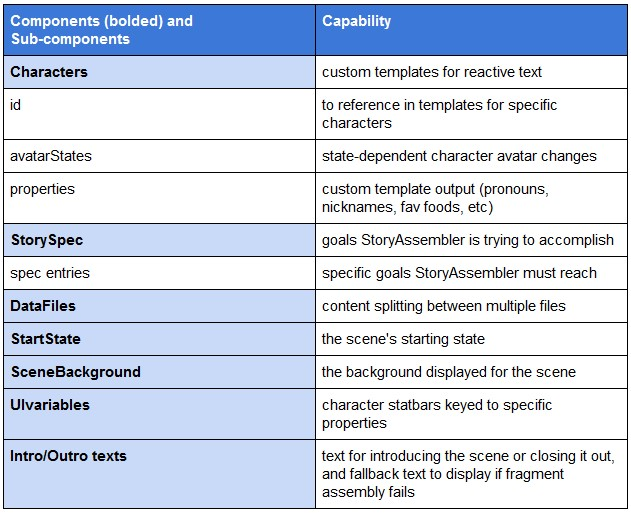
\includegraphics[width=\textwidth]{figures/3-StoryAssembler/scene-components.jpg}
    \caption{A list of required components for a StoryAssembler scene.}
    \label{fig:scene-components}
\end{figure}

%%%%%%%%%%%% END FIGURE %%%%%%%%%%%%%%%%%%%%%%%%%%%%%%%%

Some of the most critical info in this, namely the goal state, requires that writers plan out their scene before committing to writing content for it, as we did for \textit{Emma's Journey}. Unlike authoring systems like Twine or Ink, this sort of up-front narrative design can stifle creativity initially, but hopefully as scene writing continues and the goals are fully fleshed out, experimentation with creative ways to achieve said goals can provide fertile ground for writers. This is similar to our experience writing for \textit{Ice-Bound} under thematic constraints towards the end of content creation, and also echoes some of the constrained writing practices from Oulipo. Obviously, the information encoded in the config file is subject to change as the scene evolves, although the more elaborate the goal state, the more ``finicky" changing goal elements could be, resulting in ``unhappy accidents" where the system would be unable to bridge to necessary choice branches, due to pre-conditions or effects not firing in the same way.

Once the planning was done and the goal state filled out, we could move on to fragment authoring. This also could become quite complex, as more features were added to the system that resulted in additional fields needing to be written and accounted for in subsequent fragments. A list of all fragment components can be seen in Figure \ref{fig:fragment-components}.

%%%%%%%% BEGIN FIGURE %%%%%%%%%%%%%%%%%%%%%%%%%%%%%%%%%

\begin{figure}
    \centering
    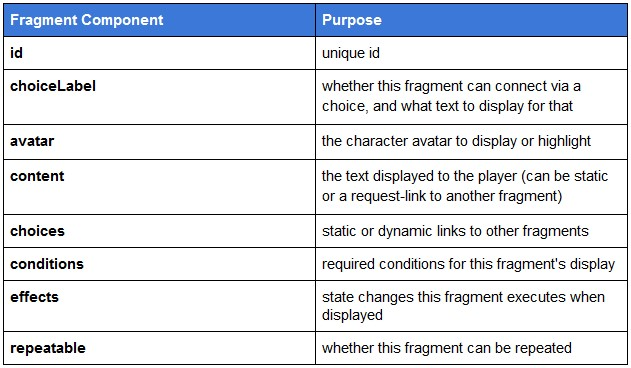
\includegraphics[width=\textwidth]{figures/3-StoryAssembler/fragment-components.jpg}
    \caption{Fragment components.}
    \label{fig:fragment-components}
\end{figure}

%%%%%%%%%%%% END FIGURE %%%%%%%%%%%%%%%%%%%%%%%%%%%%%%%%

In \textit{Ice-Bound}, there was a sense while writing that one could start with static, simple content, then add the dynamism as you went along. That way the system would get progressively more dynamic, but you would always have a ``fallback." You wouldn't fail, just successfully work with less than the desired dynamism. Common sense dictated that a similar strategy might work with \textit{Emma's Journey}.

However, we found that the difference between the simplest formulation--that of the static link fragment with string body text and choice label--did not ``play well" with more dynamic fragments (as detailed in the next section). In the end we pushed as much dynamism as we could get and still ensure a playable narrative experience, but these difficulties with the incremental addition of dynamic content meant that there were still far more static fragments in the final project than we originally intended. Our ideal fragments, composed of several interchangeable sub-fragments, remained more ``hero" content creation than anything. A diagram of a hypothetically ``maximally dynamic" fragment can be seen in Figure \ref{fig:maximal-components}.

Even if a fair number of \textit{Emma's Journey} fragments themselves were static, however, there was still the state-driven templating aspect that could change their surface text, and even statically linked fragments could be ``dynamically triggered" if they depended on parameterized goal elements, and then exposed in the scene description for the reader to change. Thus, while falling short of our initial expectations for dynamism, there was still plenty left to surprise us, given these other affordances.

%%%%%%%% BEGIN FIGURE %%%%%%%%%%%%%%%%%%%%%%%%%%%%%%%%%

\begin{figure}
    \centering
    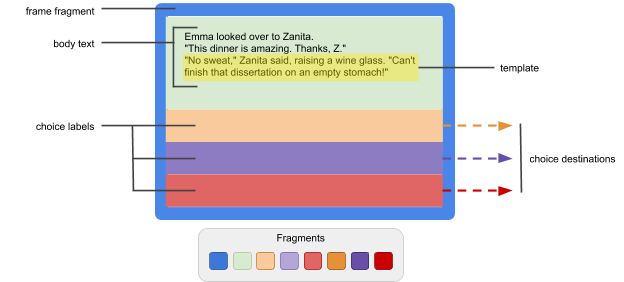
\includegraphics[width=\textwidth]{figures/3-StoryAssembler/fragment.png}
    \caption{An example 3-choice StoryAssembler fragment with eight different fragment references (a frame fragment, body text from a fragment, three choice labels and three choice destinations, each to unique fragments).}
    \label{fig:maximal-components}
\end{figure}

%%%%%%%%%%%% END FIGURE %%%%%%%%%%%%%%%%%%%%%%%%%%%%%%%%

Regardless, planning the goal state and writing the fragments to fulfill it involved a high amount of Complexity. The aforementioned issues with unintended side effects, while a product of the content creation complexity, play into StoryAssembler's most dogged authorability challenge: Clarity.

\subsubsection{Clarity}
\label{clarity}

Because of all the components required for both goal elements and individual fragments, reaching high Clarity for authors using StoryAssembler can be a stiff challenge. Because the baseline unit of content for StoryAssembler is the fragment, finishing a story ``beat" frequently, if not always, requires writing multiple fragments (not to mention the additional fragments required if one wants to provide choices, which is the point of the whole system!). This means that, when writing for StoryAssembler, the dynamics of how content is selected can never be far from the writer's mind. This is in contrast to systems like \textit{Ice-Bound} or Delve, where the individual units of content are more self-contained. This is reflected in their lower Contextuality score, and is directly tied to author's ability to author for them in a more isolated, standalone fashion.

\paragraph{Data Visualization}

As with \textit{Ice-Bound}, one thing which can greatly increase Clarity for authors is data visualization. This allows them to get a sense of what shape the story is taking, and what content needs to be authored to fill gaps in coverage.

Without a tool, the only way to double-check content authoring in StoryAssembler works is through exhaustive traversal of the choices. Due to their dynamic assembly, this means the entire structure must be re-verified with each added fragment or choice, to ensure a changed or added fragment isn't showing up in an undesired spot due to unforeseen state conditions.

Therefore, the visualization solution created for StoryAssembler needed to show three things: the assembled choice structure, when goal elements were being fulfilled, and how content was being re-used. Given that the code underlying StoryAssembler was under active development, we got our data by running a ``headless" version of the scene, and automatically traversing it. This meant that the code running for the visualization was the same as what ran the game, and changes to the engine as it was developed were always faithfully reflected in the visualization. 

The viz tool would traverse the structure in a depth-first manner, keeping a list of the choices it had not yet visited as unique entries of ``clicks" on the UI from the beginning of the scene. When it reached the end of the scene, it would go to the array, run the clicks of the next entry, and proceed from there. In the case of ``no path found" errors, it would flag that data to be represented as an error.

The resulting data was displayed as an interactive directed graph using the Cytoscape.js library \cite{cytoscape}. We chose this library because it comes with built-in graph traversal and layout algorithms, which streamlined some of the development. In addition to graph layout, other strategies were used to expose some of the underlying structure.

%%%%%%%% BEGIN FIGURE %%%%%%%%%%%%%%%%%%%%%%%%%%%%%%%%%

\begin{figure}
    \centering
    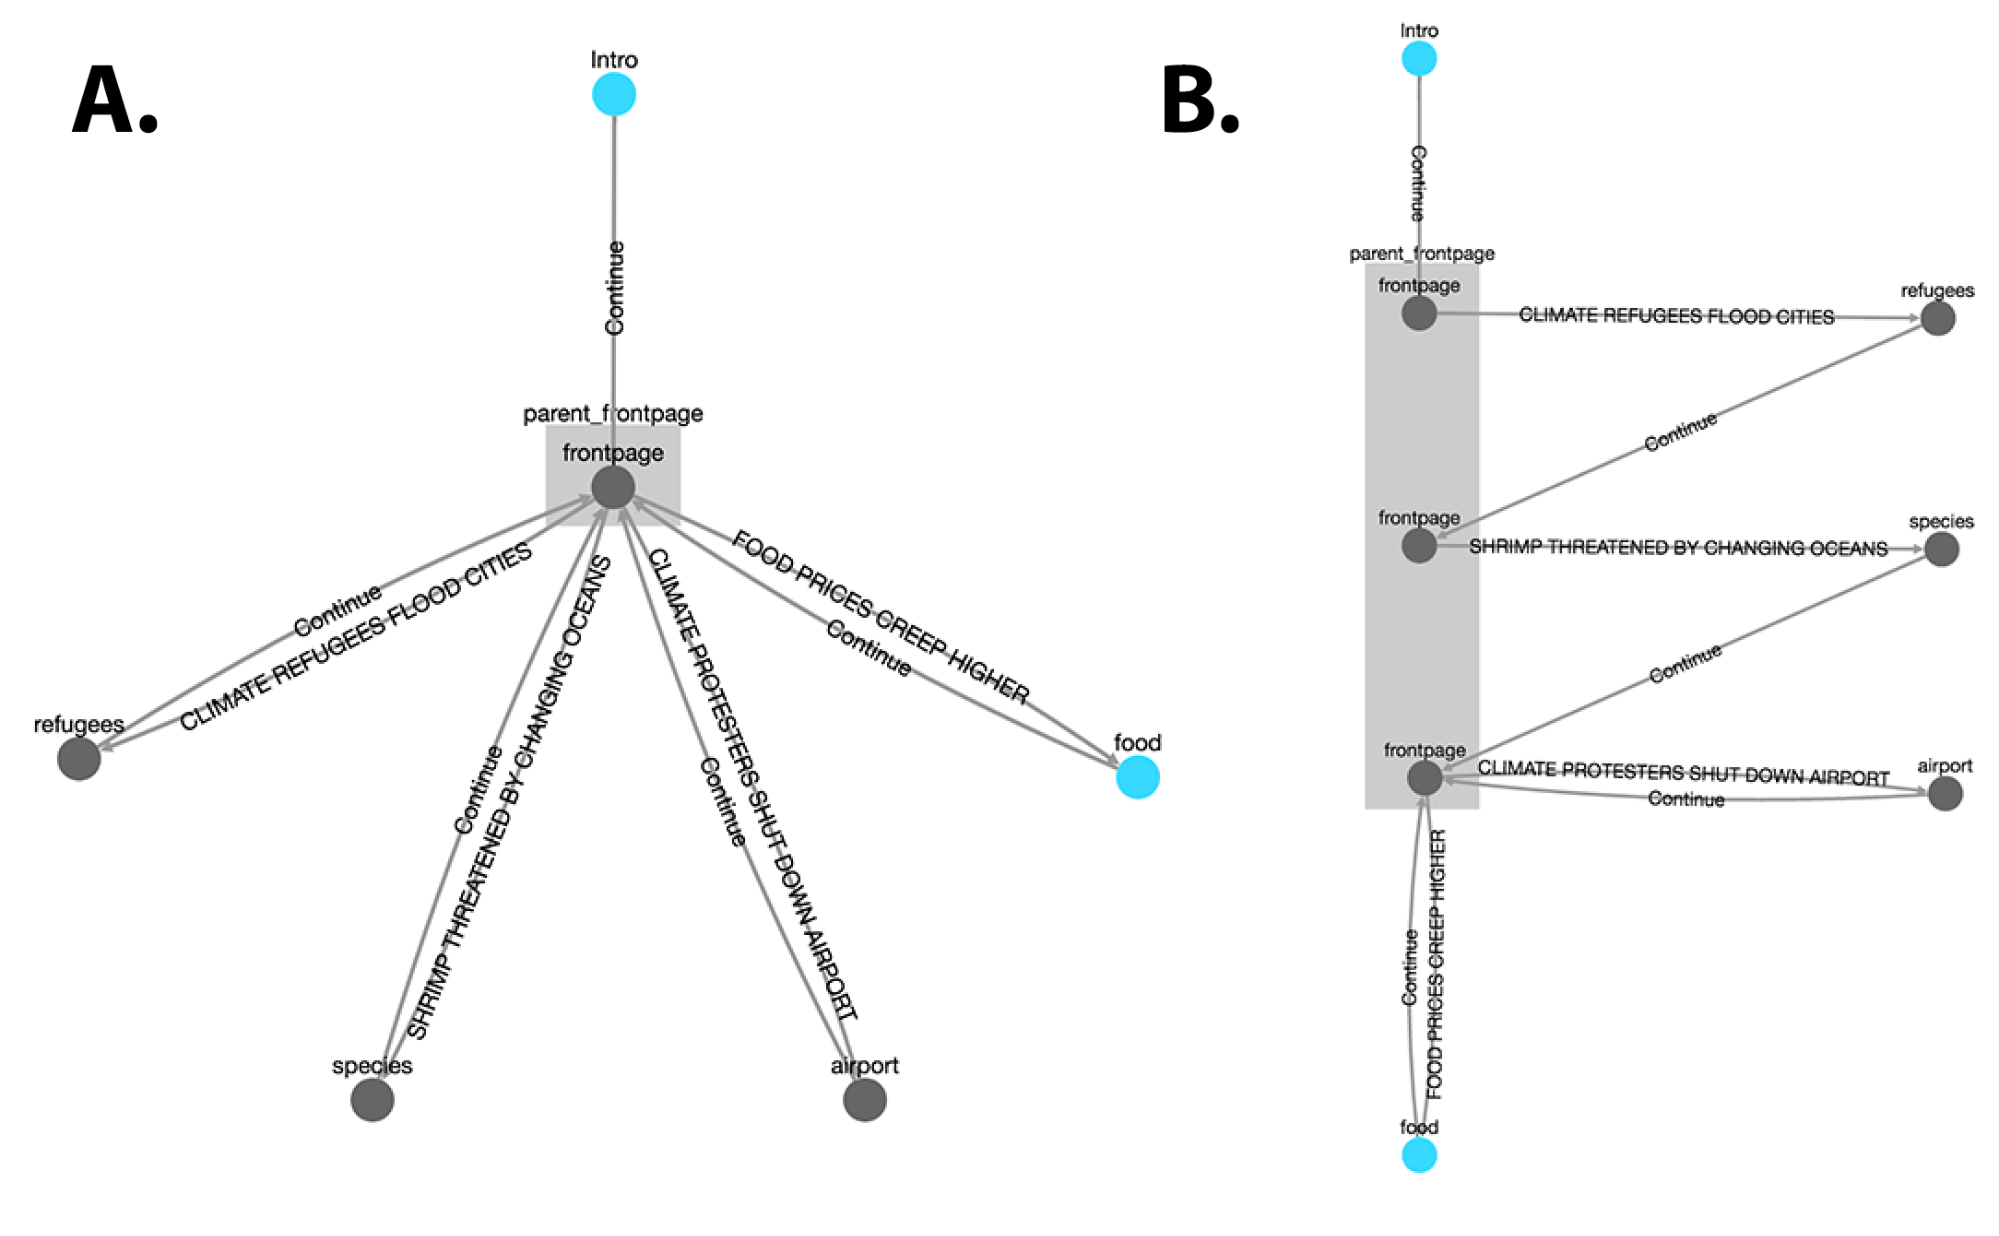
\includegraphics[width=\textwidth]{figures/3-StoryAssembler/viz1.png}
    \caption{Visualization with articlesRead as differentiating state value (B) and not (A).}
    \label{fig:viz}
\end{figure}

%%%%%%%%%%%% END FIGURE %%%%%%%%%%%%%%%%%%%%%%%%%%%%%%%%

In the visualization, we specify a subset of the narrative's state variables to establish whether a node in the structure could be considered structurally identical under different contexts. A good example is a short test segment where Emma is sitting in an airplane reading the newspaper. After an introduction (which fulfills an introductory goal element) she has a choice to read any of four articles, incrementing a state variable \texttt{articlesRead}. When four articles are read, the last goal element is fulfilled and the segment ends.

If we set the visualization to not consider \texttt{articlesRead} as a differentiating state value, we get a flower-like structure with the central node as the recurring fragment (Figure \ref{fig:viz}a). If we set \texttt{articlesRead} as a differentiating state value, however, we get a different structure (Figure \ref{fig:viz}b) where the recurring node, although identical in content, appears as a separate entry. However, they are still grouped together in a box, due to their shared content ID. This type of viz flexibility is desirable, as there are cases where authors may want to change what is considered a revisited node, in order to ensure the proper state changes are occurring. This may also be a good strategy to use in works where most of the dynamism results from state, and the viewer can toggle which variables are being considered to differentiate a node as unique.

%%%%%%%% BEGIN FIGURE %%%%%%%%%%%%%%%%%%%%%%%%%%%%%%%%%

\begin{figure}
    \centering
    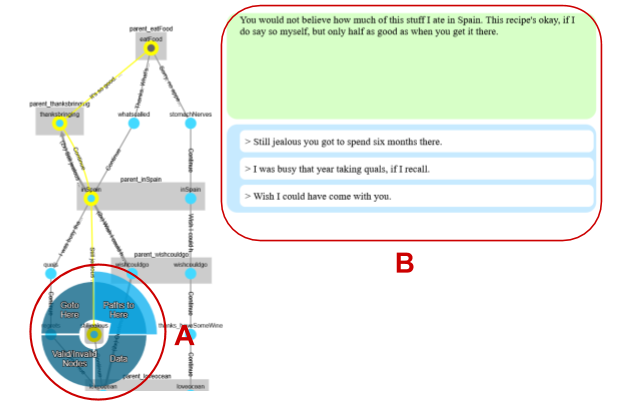
\includegraphics[width=\textwidth]{figures/3-StoryAssembler/viz2.png}
    \caption{When right-clicked, a node in the visualization brings up a contextual menu. Clicking ``paths to here" will highlight paths to this node in yellow (as shown), while also bringing up the narrative at that state (B). Valid and invalid nodes for this point of the story can also be shown.}
    \label{fig:viz2}
\end{figure}

%%%%%%%%%%%% END FIGURE %%%%%%%%%%%%%%%%%%%%%%%%%%%%%%%%

Blue nodes are used to signal when fragments are satisfying goal elements. Right-clicking nodes brings up a contextual menu (Figure \ref{fig:viz2}), allowing the viewer to highlight narrative paths through the diagram leading to this node. Additionally, the viewer can also use this menu to see which fragments were considered valid and invalid by StoryAssembler when it selected that fragment as the best fit in the progression. This was enormously useful for situations where the author has in mind a specific spot for a fragment, but it isn't currently being assembled there. They can right-click where a different node is selected, see the desired node, along with a listed state condition that failed, precluding its appearance.

Lastly, paths between nodes are aggregated into thicker lines in the case where multiple unique playthroughs traverse the same connection. This helps convey the scale of difference between main paths and unique side paths at a glance.

Because of these features, authors were able to locate out-of-place nodes in initial scene drafts quickly, and see if tweaks to those nodes (be that in conditions, effects, or some other detail) resulted in correct placement across many branches. It would also show when nodes were inadvertently orphaned by changes to other parts of the story (typically by modifying state the orphaned nodes depended on) thus saving time in some of the initial stages of scene composition.


\paragraph{Compound Fragment Authoring Patterns}

In the course of trying to navigate the particular challenges with compound fragments, we found that establishing abstract authoring patterns to copy and paste provided useful templates for writers to use. An example pattern can be seen in Figure \ref{fig:auth-pattern}, which allows for fragments to be available both as standalone beats (linked to another via a system-inserted ``continue" link) or by virtue of a ``linking choice label fragment", here seen as ``optionalChoiceLabel."

%%%%%%%% BEGIN FIGURE %%%%%%%%%%%%%%%%%%%%%%%%%%%%%%%%%

\begin{figure}
    \centering
    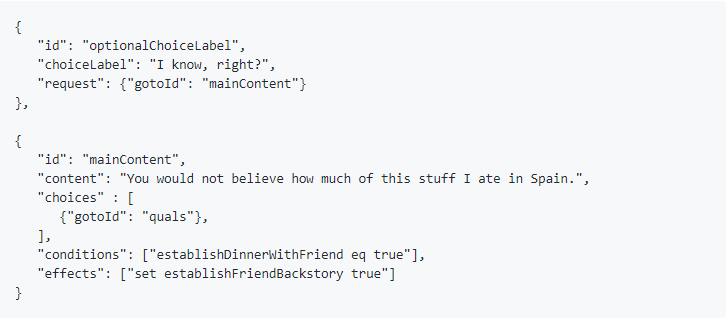
\includegraphics[width=\textwidth]{figures/3-StoryAssembler/data-object-1.png}
    \caption{A sample authoring pattern for a fragment which is available both through a choice (by way of the ``optionalChoiceLabel" fragment) and as a standalone fragment linked via ``Continue."}
    \label{fig:auth-pattern}
\end{figure}

%%%%%%%%%%%% END FIGURE %%%%%%%%%%%%%%%%%%%%%%%%%%%%%%%%

Of equal or more importance to these snippets themselves, was a paired summary of ``features and caveats" for each pattern. These ``gotchas" could frequently be unintuitive and difficult to remember, and were recurring stumbling blocks for content creation. For example, in the aforementioned pattern (due to vagaries of StoryAssembler's state evaluation system) an ``optional choice fragment" can't have effects that satisfy the main content fragment's preconditions. This is only something that would be apparent after much debugging and stepping through state logs, and not something in practice we would want our authors to have to deal with. Even describing the caveat at times could stretch a writer's ability to maintain clarity about what the fragment was enabling, but if nothing else it helped clarify system capabilities.

Over time, these system-specific patterns were aggregated in our ``writer's bible", which also contained a shorthand reference for the template syntax, dynamic goal element syntax, and other domain specific languages. The creation of such documents should be of high importance for complex dynamic narrative systems, as they pave the way for later efforts like opening up authoring to novice writers, or open sourcing the library. The writer's bible for StoryAssembler was cleaned up and formalized, and is currently available as part of its open-sourced library on Github \cite{github_storyassembler}.


\subsubsection{Controllability}

Because of our choice to pursue a narrative driven by conversation, we set up a situation with 
very high Contextuality. This in turn demands high Controllability, such that we don't generate juxapositions of content that don't make sense. This problem is compounded by the fact that, due to high Complexity, it's easy to write something in StoryAssembler with bad dynamics. This manifests itself as paths that, when traversed, result in a ``No Path Found" error, meaning the system cannot find any content that fulfills the current state conditions, while making progress towards the goal state. StoryAssembler has a boolean variable in its configuration for ``randomness" which forces it to, instead of picking the first top-scoring fragment assembly from the sorted list of possible assemblages, randomly pick from the multiple top-scoring assemblages, if their scores are identical. In very early prototypes of \textit{Emma's Journey}, however, it was so confusing and difficult to debug problems with bad content dynamics that we kept it turned off for the rest of the project, leaving it for some future date once we had the baseline content ``locked down."

This problem with complex state conditions isn't unique to StoryAssembler. Indeed, in many ways authors trade one set of problems for another when trying to systemically generate content rather than hand-author it. For example, Mawhorter noted when writing for Dunyazad stories that ``by limiting the complexity of vignettes and refreshing most of the world state between vignettes [...] the system has fewer opportunities to accidentally create plot holes" \cite{dunyazad}. However, for the task we set ourselves with \textit{Emma's Journey}, we wanted to confront the challenge directly, by pushing the complexity of individual scenes, and even having world state bleed over from one scene to the next.

When starting, our first instinct when confronting this Controllability problem was to apply strategies that normally work with systems like Twine or Ink. We thought we could first go through and write a static story graph for the scene, then go back through and slowly introduce complexity, until we reached a point where the scene's dynamicness and flexibility fulfilled our requirements (or at least until we'd exhausted our available time!).

In practice, this turned out not to be as feasible a plan as we'd hoped. Because StoryAssembler is greedily searching for fragments to fulfill goals, no matter the order, content added to increase dynamicity in one section of a narrative could break the progression in earlier parts of the scene because it technically satisfied a requirement earlier on. In reaction to this, our authors became proscriptive with state gating through flags or other variables. This uncomfortably echoes the same issues Tearse, Mawhorter, and Reed encountered when writing in Skald for \textit{Problem Planets}, where ALPs restricted the state so much, they were effectively pre-scripting the scenes.

Spierling and Szilas had a similar problem with authoring for their IDTension and Rencontre systems:

\begin{quote}
    Since it appears difficult to grasp the specifics of an engine, and therefore to ground any story design around the underlying computational models, some authors tended to use only a subpart of the engine's features. As a typical experience in first authoring
attempts with each of our engines, an author would naturally try to reduce the functionality to a linear or branching structure, which is more intuitive.
For example, the first story that was written with Rencontre by an author external to the project did not use fuzzy hypersections, which constitute one of the distinctive features of this engine. [...] In other words, the result was far from conversational storytelling. It rather resembled well-known structures of casual or adventure games \cite{authoring_issues}.
\end{quote}

There was a further problem that emerges from this. Even scene fragments that are ``dynamically linked through state" can be functionally static, if the conditions gating their appearance are only satisfiable in one way. Given the cognitive overhead of state tracking for dynamic links, authors could potentially cover ground faster by authoring several statically-linked fragments, as opposed to fewer (but more dynamic) fragments. This is the heart of the ``authoring wall" issue we introduced in Section \ref{authoring-wall}, where a dynamic unit of content that covers ten games states (but takes an hour to write) is ``slower" than ten units of static content that cover one state per piece and can all be written in half an hour.

For \textit{Emma's Journey}, we sought to get around this problem by splitting the authoring tasks into two types: structural design and implementation. As mentioned earlier, for each scene, we would go over the beats of content we wanted to be present. Then, we would come up with a structural framework to deliver that content. We would ``clump" content into more manageable segments (typically five or six per scene) and then think about how those clumps could be rearranged dynamically within the scene, while still retaining coherency.

After these sessions, we would make placeholder fragments (with no surface text, just descriptions) and link them together dynamically as we'd outlined in the diagram. Troubleshooting then could be confined purely to syntax errors and state errors, not things relating to surface text templating or other issues. The simple one-sentence descriptions for content would provide just enough context that if they appeared in strange places, it would be noticeable, but not so much that we would get distracted by trying to make transitions seamless.

After the fragments were in place and behaving correctly, we could then do a pass where writers would put in the text content, as well as the choice labels and other components. The final pass was for injecting more dynamism or smoothing transitions using state-based templating, or trying to add more choices to flesh out the dynamic core, even if said choices provisionally only had a few different ways they could link. At the least, they provided easy ``hooks" for returning later to add even more dynamism. The main focus of our design centered around increasing dynamism for the ``beats" satisfying the goal elements.

This tactic of structural design meetings up front also enabled us to divide labor between scene beats, and the capability to combine libraries of content between files meant that writers could then go off separately and create content to fulfill them, knowing what the other beats would be in the scene, and a rough idea of what they would entail. Writers could also coordinate on state changes they wanted to make in their section, and which variables were available for them to use to customize the state templating to make the text more reactive to player choice and gameplay. Then, a final editing pass was done once they brought their files together to smooth out rough edges.

\subsubsection{Authorability Summary}

The challenge set before us by \textit{Emma's Journey} was a steep one. While (from a technical format perspective) content creation for StoryAssembler is very similar to \textit{Ice-Bound}, the Proficiency required for the specific case of this project extended beyond software. It provided an exciting opportunity to head up a ``writer's room" of novice writers engaging with procedural authoring, with its own set of issues that comes from any project management endeavor. StoryAssembler's capabilities to enable collaboration between multiple writers on single scenes helped ease the pain points, but careful planning was still required from a narrative design standpoint, making this a medium Proficiency endeavor.

In comparison with \textit{Ice-Bound}, StoryAssembler's fragment construction driven by goal elements is far more complex to author for. Additionally, it has all the surface text templating complexities of \textit{Ice-Bound}, but also potentially applied to the goal state itself, in addition to the content. Therefore, on the standpoint of content authoring (excluding issues of narrative design) StoryAssembler has high Complexity.

Because we had high standards for the Contextuality of the narrative, and we chose to pursue a story mediated through character dialogue, we set ourselves a requirement for high Controllability. Many of the most pernicious problems writing for this system came from the juxtaposition of fragments with effects that would invalidate later fragments, meaning seemingly-innocuous changes could have outsize effects on the story as a whole.
%%GDoc comments%%
Navigating the proper arrangement of these fragments to satisfy goal elements, all while having to keep in mind changing variables affected by the mini-game, was very challenging. Additionally, we needed to push away from static linking (whether explicitly static by linking through id, or by implication through there only being one valid fulfillment of the state-driven call). While we tried to mitigate this with visualizations, their full development lies with future work. All these factors taken together gave StoryAssembler low Clarity. 
%%GDoc comments%%
We also found that StoryAssembler's ability to support both static and more dynamic authoring meant that, when hard-to-find narrative bugs manifest due to low Clarity, authors tend to reduce the procedurality of their story structures and link choices together statically just to ``get something reliably working''. Essentially, authors have a comfort zone for authorial Proficiency and Clarity, and will reduce content complexity to stay within that zone. Given that we wanted to push the dynamism as much as possible, this capitulation over time somewhat undermined the long-term dynamic goals of the project. Our JSON editor attempted to lower required Proficiency, and the visualization tried to increase Clarity, but tool enhancements were needed to reliably represent more complex structures in longer narratives, which is exactly where authors need the most support. For the editor, an example is the aforementioned issues with edge cases in complex fragments (with dynamic choices or content compounded from several nodes). For the viz, a particularly thorny example is how best to represent the traversal graph where the indexicality of each node (fragment) is very high, but differentiating between different cases of state-dependent linkages is very important.

In the future, this might be avoided by treating authoring requirements and system capabilities more as equal partners. For \textit{Emma's Journey}, it might have served better to balance complexity such that the authoring tools kept pace with system capabilities, rather than extending system capabilities beyond the reach of the authoring tools. While we did push the dynamism of the system a great deal, complex structures many times required extensive ``design debugging'' to ascertain why certain content was being displayed at certain times, which cut into time that could have been used to deepen the narrative content.

\textit{Emma's Journey} was a valiant first effort, but StoryAssembler is capable of even more complex narrative dynamics, \textit{if the clarity while authoring enables it}. These could enable potentially new experiences, but equally valid would be focusing work on better supporting the basic authoring patterns and capabilities, until such authoring becomes more tenable.

\subsection{Future Work}

After \textit{Emma's Journey} was finished and released, StoryAssembler was extracted from the game's codebase, and roughly formulated into an open source standalone JavaScript library \cite{github_storyassembler}. While functional, it's still in its early stages, with a few key expressive capabilities from \textit{Emma's Journey} left to be abstracted and formalized for reuse in other contexts. It's hoped that with further development it will become an attractive beachhead for practitioners seeking to tackle problems in a similar space.

Of particular interest is the further development of authoring tools similar in sophistication to the \textit{Ice-Bound} visualizations that could help increase Clarity for authoring with the system. StoryAssembler's capabilities have not yet been fully plumbed, and so the next ``technical push" in terms of the system must be for systemic authoring support tools, such that the unexplored capabilities can be leveraged for new types of interactive experiences.

In the realm of more wildly ambitious possibilities, the StoryAssembler system has been extracted while preserving the separation between the HTN-like planner system (internally called bestPath) and the general forward state-space planner that calls it. It may be possible, if the code is further segmented and abstracted, to ``substitute in" different algorithms to either of these systems, in order to even more widely explore its systemic dynamics, perhaps as more a platform for telling stories than an individual system. Integration of systems such as a javascript port of a Prolog interpreter or a JSHOP-style planner would enable intriguing new explorations, though they would undoubtedly come with their own content authoring complexities and concomitant issues.

\subsection{System Summary}

\textit{Emma's Journey} had ambitious desired features which set us up for a difficult authorial challenge. It was of \textbf{medium Explorability} and \textbf{medium Replayability}, because we wanted players to both be able to explore different states through performance with the mini-game, and also go back to try scenes multiple times to make different choices, or experiment with different starting conditions. Unfortunately, due to the \textbf{high Complexity} derived from the complex interplay between hierarchically-assembled fragments and the goal elements, we weren't able to reliably author fragments that were reusable across many different contexts, leaving us with \textbf{low Reusability}. Finally, the demands of the specific narrative format of \textit{Emma's Journey} meant that fragments needed to be tightly connected and avoid nonsensical juxtapositions. We did not have the benefit of a forgiving frame narrative as in \textit{Ice-Bound}. Therefore, we were setting ourselves up for a \textbf{very high Contextuality} requirement.

In order to meet this challenge, we tried to keep the proficiency requirement as low as possible. However, the choice to engage a team of writers, rather than two writers also doubling as system engineers as in \textit{Ice-Bound}, meant that our requirements for teamwork and collaborative narrative design pushed us to \textbf{medium Proficiency}. The expressiveness of the system, driven as it was by the various possible fragment assemblages and goal state possibilities, meant we also had a \textbf{high Complexity} problem. This was compounded by the emergent narrative dynamics, which made it difficult when adding content to predict how other content in the scene would then be assembled. We tried to ameliorate this through the use of some system-specific authoring patterns and an initial attempt at a visualization tool, but StoryAssembler remains a challenging system with \textbf{low Clarity}. Future work hopefully can develop these tools further, in order to enable authoring which can leverage its full potential.

\subsection{Next}

Despite the challenging hurdles \textit{Emma's Journey} presented, we were able to overcome them to offer a completed experimental research game which generates choice-driven narratives in concert with generated mini-games, all working together to create a unified, compelling experience.

Both \textit{Ice-Bound} and StoryAssembler were combinatoric, leveraging their systems in a similar approach to juxtapose content together based on pre-condition logic and blackboard state, though the final expression of that form (and how that juxtaposition was controlled) differed greatly.

However, what if one could take such approaches, but apply the combinatorics to ``pattern match" to a simulation of already existing events? And what if one pushed on that symbolic connection between simulation and narrative representation, to make even the connection itself  something which could be procedurally manipulated?

This is the motivating premise of the final group of prospective systems and prototypes, each an exploration of a similar approach, using a different methodology: \textit{LegendWriter}, \textit{Argosy}, and \textit{Delve}.

\chapter{Delve}
%\section{section} (h2)
%\subsection{subsection} (h3)
%\subsubsection{subsubsection} (h4)
%\paragraph{paragraph} (h5)
%\subparagraph{subparagraph}


%%signposting%%
\textit{Delve} is a narrative game currently in development. Its main interaction is player manipulation of objects in a 3D environment to influence character memories. Initially the research focus was on generating simulation events which could be narrativized and instantiated as metaphorical objects in a 3D environment. However, enough fruitful insights and challenges were generated by development of the narrativization system itself that it was eventually decided to reduce the scope of the project to just the narrativization system, and decouple it from the simulation. In comparison to \textit{Ice-Bound} and StoryAssembler, \textit{Delve} is system-complete but not content-complete. Thus, it affords an excellent opportunity to show how the Authorial Leverage Framework can inform design decisions before authoring has begun in earnest.

As with \textit{Ice-Bound} and StoryAssembler, we'll first detail the experience challenge we hoped to tackle. Then we'll detail related works in similar spaces. Because initial \textit{Delve} prototypes involved simulation-driven narrativization, we'll look at similar systems in Section \ref{subsec:simulation-driven-narrativization}. We'll then introduce Expressionist in Section \ref{subsec:expressionist}, J Ryan's system for surface text production which was used to generate the memory text. Last, because \textit{Delve} makes use of an ontology to connect between text production and object state in a metaphorical manner, we'll talk in Section \ref{subsec:computational-metaphor} about other works that have used similar techniques for a variety of aims.

We'll then discuss two prototypes that informed \textit{Delve}'s development, and yielded insights into simulation-driven narrativism. The first is \textit{LegendsWriter} in Section \ref{subsubsec:legendswriter}, a prototype that generates stories from \textit{Dwarf Fortress} game logs. We'll also discuss \textit{Argosy} in Section \ref{subsubsec:argosy-and-sculptural-sifting}, a game where the narrativism is leveraged as a player interaction mechanic. 

Having introduced these works, we'll be well-positioned to tackle \textit{Delve}'s system architecture in Section \ref{sec:delve-system-description}. Having detailed that, we'll then be able to talk about specific implementation details in Section \ref{subsec:delve-implementation-details}, leading to content creation in Section \ref{subsec:content-creation-for-delve}. With all this contextualized, we will in conclusion show how the application of the Authorial Leverage Framework applies to \textit{Delve}'s content challenges. In Section \ref{subsec:delve-traversability} we'll detail the Traversability challenges it poses, and in Section \ref{subsec:delve-authorability} how different design choices can be made within the constraints of the implemented systems to lessen the authorial burden for the upcoming content creation push.
%%signposting%%

\section{Experience Challenge}\label{sec:delve-experience-challenge}

\textit{Ice-Bound}'s system has no simulation. Its ``starting state" is whatever effects run on fixed symbol cards for a given level, and whatever themes the player has picked so far. This is less a simulation than a record of play so far, or initial constraints for story generation.

\textit{Emma's Journey} has some light simulation. Each level has a starting state for the blackboard, and each fragment can execute effects. One could make a simple simulation from these materials with each fragment executing some state change, though making such a low-grain simulation the focus of the system would be considered an ``abuse", and outside the primary aim of it. In \textit{Emma's Journey} it functioned much the way \textit{Ice-Bound}'s blackboard did: a simple record of which choices the player had made so far, available to be logically operated upon to filter future content. 

Peculiar to \textit{Emma's Journey}, StoryAssembler interfaced with the \textit{Gemini} game system \cite{summerville2018Gemini} and updated fragment text and choice availability based on a few variables that continuously changed while the mini-game was running, which could be considered a ``simulation" of sorts. But again, leaning heavily into that direction would also be outside the intended use of the narrative system.

But what if we had a narrative system that had simulation considerations ``baked in"? How can we incorporate the combinatoric design considerations of \textit{Ice-Bound} with the goal-driven capabilities and considerations of StoryAssembler within the context of a narrative simulation?

The system created to explore this narrative possibility space was \textit{Delve}. Two exploratory systems (\textit{LegendsWriter} and \textit{Argosy}) were made along the way to explore some of the affordances and implications of simulation-driven narrativization, one of the core areas \textit{Delve} engages with. \textit{LegendsWriter} and \textit{Argosy} are prototype systems created to narratively illustrate independently-operating simulations. These simulations generate a series of events according to their own logics, with their own set of considerations. The generated record of the events composes an intermediary data object. The narrative systems then use that data object to guide character story creation, threading the needle between the expressiveness of human-authored narrative, and the emergent state arising from the simulation. This approach is more ``bottom-up," because it is working to build narratives up from individual pieces, matching patterns from each step of the simulation.

After realizing how rich a simulation would be required to provide adequate material, we pivoted for \textit{Delve} to explore the idea of generating history through more of a ``top-down" method, where simulation steps are paired with narrative pieces, but the scope of the simulation goes from large to small. For example, the first step of the simulation is to find a general event which can encapsulate the totality of the time period being simulated, which is then subdivided into smaller and smaller sub-steps until it gets to individual timesteps. This afforded us more narrative control, without requiring fine-grained simulation from the get-go.

The desired play experience for \textit{Delve} necessitated taking that system further, however, as this process was meant to enable an interactive---not passively generated---experience. To accomplish this, Expressionist grammars \cite{ryan2016expressionist} (covered in Section \ref{subsec:expressionist}) are used to generate the surface text for character memories. These grammars, along with their semantic tags, are output as an intermediary data object. A translation system converts these tags to new values, which are consumed by a second system in order to create instantiated, interactable 3D objects. 

The ambitious intent with this was to create not only a system that could generate character histories, but also represent them symbolically via interactable objects in a 3D game, specifically through the lens of the \textit{method of loci} or ``memory palace", a visualization technique that dates back as far as Cicero \cite{Herrmann1988}. Said objects could then be manipulated by the player, and thus the ``memories" of the character in question could be modified, given the translation of the object's state change back into the narrative space, through the symbolic mapping (implementation details are expanded upon in Section \ref{subsubsec:delve-implementation-memory-palace-generation}).

This sort of experience would allow the playful exploration of the narrative possibility space of a character's memories, but through a level of symbolic and metaphoric remove. The main drive of gameplay would center around getting character memories into certain states, through a process of experimentation to determine what the metaphoric mappings were. These memory manipulations would pose ``mnemonic puzzles", where the player would need to figure out how to either restore or mould a character's past to a particular state, in order to reveal critical bits of the overarching narrative. This is similar in gameplay design to Horswill's \textit{MKULTRA} \cite{horswill_MKULTRA}, an AI-driven game which allows players to modify NPC beliefs through ``brainwashing" to accomplish level goals, such as retrieving an object the NPC wants to keep hidden.

These are \textit{Delve}'s long-term plans, but our first goal was building a system enabling such content to be created in the first place, so that the feasibility of the gameplay experience (and the authoring it required) could be explored. This goal was achieved, though authoring of content has yet to begin in earnest. Thus, this section will be focused on details from development of \textit{Delve} to the stage of ``all systems prototyped and operational", as well as talking about useful insights gained from two prototypes (\textit{LegendsWriter} and \textit{Argosy}) along the way. We will then show how applying the Authorial Leverage framework to \textit{Delve} before substantial authoring starts can help identify key forthcoming challenges, and suggest design and tool approaches to make authoring for \textit{Delve} more tractable.

\section{Related Works}\label{sec:delve-related-works}

\textit{Delve} touches on topics covered by a wide field of systems. Generally speaking, they fall into two broad categories: simulation-driven narrativization systems (relating to how it generates memories for characters), and computational metaphor systems (relating to how it represents them to the player). It also makes use of J Ryan's Expressionist system, which generates the surface text of memories, as well as provides the connective tissue between the two categories through semantic tagging.

We'll first talk about simulation-driven narrativization, which generates narratives using event logs from simulations. Then we'll talk about Expressionist, a system that leverages semantic tagging on grammar output to generate text. In the case of \textit{Delve}, the semantic tagging of simulation event text bridges us to the last step: translating it into a new form. The related work in ontologies and computational metaphor situates that translation process, by showing how previous efforts have been made in systemic content transformations through the use of such approaches.

\subsection{Simulation-driven Narrativization}
\label{subsec:simulation-driven-narrativization}

``Simulation games" is a broad categorization that encapsulates a variety of works made for many different artistic and entertainment goals. However, we are concerned here not so much with their form, but their \textit{substance}. Which is to say: their event data. Specifically, we are concerned with both how simulation games represent their interior events to the player, and also how third-party, external systems can make use of exported event logs to then construct post-facto narrativizations of what happens within the game.

Narrativization of games has a rich history rooted in both computer science and narratology. Most salient to our immediate purposes is ML Ryan's 1993 work on narrative in real time \cite{mimesis_baseball},  which provides a highly useful conceptual framework for thinking about how these processes interact. In it, she divides narrative into three aspects:

\begin{enumerate}
    \item the chronicle (the \textit{what}, enumerating events)
    \item the mimesis (the \textit{how}, transporting readers through description)
    \item the emplotment (the \textit{why}, the logic and design making events sensible)
\end{enumerate}

ML Ryan's framework is presented in the context of listening to a live broadcast of a baseball game and forming a narrative of what's happening, a task directly mappable to many systems through the years---up to recent efforts---that we will shortly enumerate.

ML Ryan also emphasizes a key distinction in her framework between \textit{real-time} and \textit{retrospective} narrative acts, and the tension between being able to substantially provide plot when future events are not known, versus the increased importance of plot to provide a \textit{reason} for the events to have been worth telling a story about. For example: we don't necessarily know whether a baseball game will hinge on a particular critical play. When the play first happens, the focus is on the chronicle, or \textit{what}, of it. We may also have an equivalent emphasis on \textit{mimesis}, to try to transport listeners to the stadium, so we hear the roar of the crowd, the crack of the bat, the cry of the umpire. But the emplotment, the \textit{why}, the significance of that particular play within the arc of the game, isn't wholly known---and won't be known!---until the game concludes.

However, a newspaper or announcer trying to entice people to view a game that has already concluded, will leverage all the persuasive powers of emplotment to promote the event as narratively engaging---perhaps employing some well-known tropes such as the big come-back, the upset of a champion, etc. That is, they will apply an \textit{interpretation} onto the chronicle of events to present a compelling \textit{why} of the game---how it fits into the narrative of a season or a particular team. And they will do this by (among other methods) choosing specific events in the chronicle to emphasize and report, and others to minimize or discard. This emphasis is most easily accomplished by levering a heightened \textit{mimesis} of the given events, to render them in more exquisite detail. ML Ryan's idea of history as an interpretive storytelling act is drawn and elaborated from White's earlier work on interpretive historiography \cite{white_1973}.

Therefore, this tension between chronicle and emplotment comes from an inability to predict the future. Even if we had perfect knowledge of all the events currently happening as they happened (a thought experiment Danto called the ``ideal chronicler" \cite{danto}) we would still be unable to make full use of whatever interpretive frameworks we can bring to bear on a situation. As an omniscient baseball announcer we may relate all manner of information, but despite our awesome hypothetical powers, what we \textit{wish} for is a specific set of events to happen next, a narratively charged pattern that can both make the events in the past have dramatic shape and sense, and forecast the potential of exciting developments in the future. We know the types of narrative we would \textit{like} to occur---for example, rooting for the underdog to upset the current champions---but it is impossible to tell whether that story will be the story of the game we are experiencing until certain events in the chronicle have happened.

To that related end, there's a rich seam of narrativization work in games centered around the creation of stories from chronicles of sports games, running the gamut from more traditional symbolic AI methodologies to machine learning-driven approaches, for both real-time and offline use cases. While the domain may be different, the system application and techniques are generalizable to the task of story generation from game simulation events.

\subsubsection{Live Commentary and Compelling Chronicles}\label{subsubsec:live-commentary-and-compelling-chronicles}

The Robot World-Cup Soccer (RoboCup) Simulation League is a virtual outgrowth of a physical robot competition of the same name, established in 1997 \cite{robocup} to provide a lively competitive environment to stimulate AI research on a variety of fronts. A rich community of AI researchers sprung up around it---initially for the multiple challenges of physical robot soccer. However, with the use of a server that provided the ability to stage virtual matches and export state data from them, a new opportunity presented itself: match commentary.

Three initial systems stand out for their sophistication, each from different labs: Rocco, Byrne, and MIKE \cite{andre2000three}.

Rocco is an expansion on a late 1980s prototype from the German Research Center for Artificial Intelligence (DFKI), used for automated descriptions of short soccer scenes. It was augmented by later work that resulted in a generic architecture used for multimedia reporting that could handle transformations from visual data to various styles of output, such as television-style reports and newspaper articles. To accomplish this, it used an ``incremental discourse planning mechanism", which would consult a library of previously coded knowledge on kicks or movement to match the input state, and at each increment of a time counter, calculate event salience. If no events were available, it would substitute random background information.

Rocco used state-driven templating for the generation of its surface text. The template library was hand-coded from 13.5 hours of televised soccer reports with metadata such that it could appropriately select them based on available time, bias, and report style. Rocco used a simple emotion model which could flag to change the pitch of its text-to-speech module, to communicate the agent's excitement level.

All three systems' output was speech, which introduced some productive constraints for their commentary creation. It forced not only a hard cut-off filter for events (a sports commentator can only speak so fast) but also by implication a \textit{saliency} issue---if the play had moved on while more was still to be said about a certain player or team's actions, the time to report it was lost.

Byrne, from Sony CSL, pushed the commentator aspect much further. In addition to speech, it also featured an animated head, which could express emotions while it relayed commentary. These emotions were controlled by the emotion-generation module, which managed a hierarchy of emotions ranging in intensity (1-10), a target or cause (a player action) and a decay function so they faded over time. The commentator also had a simple nationality character model, which would give it a team it supported, and some other simple variables to affect reaction emotions.

Again, because of the bandwidth constraints of speech, Byrne pruned its matching events by using a priority-scheduling algorithm. In addition to priority, events also had a ``birthday" (when it was added to the queue) and ``deadline" (when it would no longer be relevant) which were used to keep the collection of valid events fresh and topical.

The last system, MIKE, came out of the Electrotechnical Laboratory (ETL). It has the most sophisticated textual output, driven by six game state evaluation modules running simultaneously, operating at different levels of analysis. This might range from basic events (``Red3 collects the ball from Red4") to more high-level analysis like player performance evaluation (``Red1 is very active because, Red1 always takes good positions") and multi-agent strategy (``The Red-Team's formation is now breaking through enemy line from center").

Each commentary fragment is modeled as a proposition, and all modules put their fragments into one pool with importance scores, which gradually decay over time. The system selects the most salient proposition, passes it to the natural language generator, and then updates the currently active subject back to the system, to help adjust priorities for subsequent utterances. This system was later adapted by ETL into a navigation system for the blind, making use of these core architectures.

The domain of generative commentary extends to many other sports, such as horse racing. For example, systems like DEIRA \cite{deira} focus on the realism and emotional model of the commentator, using simple pre-conditions to trigger narration events, which are then grounded out using context-free grammars enhanced with state-driven templating.

The multi-agent architecture approach of MIKE has also inspired similar implementation in different contexts. Fielding et al \cite{embodied_agents} adapted a similar architecture to put actual reporters into the game as neutral players in an \textit{Unreal Tournament} capture the flag game, which then report back their observations to \textit{other} agents acting as ``editors", towards the goal of generating reports on the in-progress grame. This approach was later developed further by Tallyn et al to output both a live chronicle of the match (which more resembles a game log than human-like narration) and a longer narrative match summary \cite{embodied_agents}.

\subsubsection{Post-Match Summaries}\label{subsubsec:post-match-summaries}

There is a different thread of work for post-facto narrativization of sports games, more salient to our project with \textit{Delve}, as they operate on completed matches, and thus are released from the challenging (while productive) constraint of ``liveness", which not only limits processing time, but also the amount of emplotment that can be deployed, given the uncertainty of outcome.

Rhodes et al \cite{sports_freytag} took the example sports commentary themes from the aforementioned Ryan (\cite{mimesis_baseball}) and instantiated them through the lens of Freytag's five stages of dramatic structure \cite{freytag}, though the rise and fall of the action was replaced with the rising and falling emphasis of a particular theme. Rhodes used Lexicalised Tree-Adjoining Grammars (LTAGs) \cite{joshi1997tree} for surface text realization, which let him surface state information while avoiding repetition through the liberal use of random synonyms, which can be tweaked for intensity. While it would be a stretch to say it's on the level of color commentary, it is an interesting application of multi-event thematic progression tracking, through the application of a narrative formalism.

A couple years later in 2010, automated sports commentary was ``in the wild" with Statsheet, a sports commentary company which launched 345 websites to cover all the basketball teams of the NCAA Division 1 college basketball program, completing the task of generating over 15,000 game summaries a month \cite{statsheet}. This caused quite a panicked splash in the sports journalism community, especially in the medium of match reports, which in format are more akin to a chronicle to any sort of dramatically told story. The well-justified worry was that automated processes could provide the same level of summary with a breadth of game coverage that isn't easily achievable using human writers.

Concurrently, another sports writing website, BigTenNetwork, was also making use of a system called StatsMonkey \cite{statsmonkey} to generate match reports. StatsMonkey's architecture is centered around techniques sports reporters might use to describe a game, reified as 35 ``narrative angles", which were informed by Schank's concept of thematic structures. The events of the game are filtered by three central baseball statistics that allow them to calculate saliency values over multiple game events:

\begin{itemize}
    \item \textbf{win probability}: the likelihood of a team winning the game given the current game state
    \item \textbf{leverage index}: the historical likelihood a given event can alter win probability
    \item \textbf{game score}: a composite value to select the best players
\end{itemize}

In order to generate a match description, StatsMonkey determines a narrative angle prioritization, informed by these multi-event heuristics, and uses that, along with state-driven templating, to generate the natural language. While example output text is still succinct and seems to lack narrative concerns, these principles can be seen on display in the following example given by Allen et al \cite{statsmonkey}:

\begin{quote}
    Friday was a great day for Indiana’s Michael Earley. He hoisted the Indiana Hoosiers to an 11-9 victory over the Northwestern Wildcats (20-26). Earley blasted two home runs for Indiana (22-21). The senior right field went 3-for-5 in the game with four RBIs and two runs scored. Earley homered in the first and second innings.
\end{quote}

StatsMonkey in this case analyzed the game states and determined that Early was the most report-worthy aspect of this game, matching the ``narrative angle" of a single player carrying the team to victory, and appropriately prioritized the summary to feature him, pruning out reporting of other events as not salient to the given angle selected.

%%GDoc comments%%  
% Re-located to proper section
In more recent work involving video games as opposed to sports matches, \textit{Bardic} \cite{barot2017bardic} is a 2017 flagship system for the Liquid Narrative Group's \textit{Narrative for Sensemaking} project, which seeks to generate multimedia narratives from underlying structured game data. \textit{Bardic}'s target game was \textit{DOTA 2}, a popular multiplayer battle arena game \cite{dota}. Its goal was centered around providing several different modalities of gameplay narrativization, in order to convey different dynamics of the underlying gameplay data. For our purposes we are concerned chiefly with how it creates small stories from game logs, though it also provides generated video and a sophisticated visualization and querying tool.

To do this, \textit{Bardic} takes a game log from \textit{DOTA 2} which provides snapshots of game state at a rate of 30 times a second, with each game state containing all the attributes of each played character. Separately, the game log also includes a list of every action in the game (for their typical playthroughs the researchers dealt with roughly 60k game actions). That data then goes through a number of processes to translate and augment it, resulting in a formatted dataset. \textit{Bardic} uses an intermediary language called \textit{Impulse}, a logic-based language for narrative encoding \cite{eger2015impulse}. \textit{Impulse} represents data as \textbf{facts}, which are changed by \textbf{actions} over time, and which concern \textbf{actors} and \textbf{objects}.

\textit{Bardic} also contains hand-authored event pattern matching sequences, called \textbf{narrative tropes}. The version of \textit{Bardic} reported in \cite{barot2017bardic} contained four initial tropes (though the team expressed a plan to add more in the future): 

\begin{enumerate}
    \item chase fight (one character fleeing while being attacked)
    \item alpha strike (many on one)
    \item hard work montage (repeated actions to achieve a goal)
    \item failure montage (multiple actions and failing to reach a goal)
\end{enumerate}

\textit{Bardic} then takes a user-selected subset of this data, and---given a list of which valid narrative tropes to apply---uses a planner to filter events to the subset that fit that trope. Once achieved, it grounds out the event symbols (such as characters or properties) to surface text.

The output text is simple and descriptive. For example: ``Dazzle was a main-actor. He damaged Crystal Maiden for 22 damage with a poison touch. Then he moved from the Radiant Base to the Bottom Inner Radiant Tower. Next he damaged Crystal Maiden for 22 damage with the poison touch. Then he killed her because he damaged her for 22 damage with the poison touch. Next he healed Wisp for 25 damage. Then he died" \cite{barot2017bardic}.
%%GDoc comments%%  
%%GDoc comments%%
This is still an active area of inquiry, with efforts like Shah et al's work in 2019 \cite{shah} tackling commentary generation for ``Let's Play" videos of \textit{Minecraft}, using a convolutional network. However, for our purposes we are more concerned with output resembling well-formed narrative in its own right, rather than simply descriptive sequences of game events. That said, these systems and the formalizations they employ to achieve their generative goals are potentially fruitful lessons in techniques that could be applied to such a task.
%%GDoc comments%%

\subsubsection{Playthrough Retellings}\label{subsubsec:playthrough-retellings}

Other formalisms have been used to convert playthroughs of simulation games to story in a more structured way. Antoun et al \cite{antoun2015generating} tackled creating narrativizations of the high school drama simulation game \textit{Prom Week} \cite{mccoy2012prom} using story intention graphs (SIGS) \cite{elson_SIG}, a semantic narrative representation that has been applied by other researchers to other works such as TellTale's \textit{The Wolf Among Us} \cite{Murray_wolf}. While their work remained somewhat proof-of-concept, Antoun et al's approach was to automatically derive structured plot data from harvested playthroughs of the game. Unfortunately they found in the pursuit of this that, while with some effort on their part they were able to encode the features of playtraces into SIGs, the stories generated by the playthroughs lacked coherence. This potentially could have been due to a feature mismatch of the SIG specification and the underlying simulation of \textit{Prom Week}, which made translation between the two difficult. Regardless, the approach of taking a technique usually deployed to hand-encode stories for analysis, and attempt to backchain it instead to generate stories from structured data, is a compelling thread of research.

So far we've seen how third-party applications might make sense of a game, whether that be baseball, horse racing, first-person shooters, or high school social simulations. However, there are also games which generate and represent their own histories to players internally. This is also useful for us to examine, as it directly relates to surfacing simulation state in a narrative manner.

\subsubsection{Internal Representations: History as Process and Artifact}\label{subsubsec:internal-representations}

Simulations are excellent event generators. Their positioning as a cohesive world, even if fictional, means that their events suggest an authoritative history, or at least a historical chronicle. But because history is intrinsically the process of meaning-making, a simple recording of events isn't enough to relate a story. As put forward by ML Ryan and White, that requires interpretation. In our case that might mean the person reading the record, or perhaps other processes within the game.

There are some illustrative simulation games that pre-generate events to create their worlds. When a player starts a game of \textit{Caves of Qud} \cite{qud}, an indie procedural rogue-like game, the system first generates the history of the world up to that point, populating the sultans and their respective historical domains, and using that to drive other processes to formulate groups and societies, complete with rivalries and alliances. Grinblat and Bucklew, the creators, are very conscious of the choices made to create this historical narrative, and broadly categorize two different approaches to simulating history in games: history as process, and history as artifact:

\begin{quote}
    There’s a distinction to be made between history as a process and history as an artifact. The former can be conceptualized as the playing out of rules and relationships that continually produce the present. To simulate this process, we might seek to reproduce its logic. On the other hand, the latter is a constituent of the present, something we engage with through a contemporary lens and whose complexities may be obscured by that flattening of perspective. \cite{grinblat2017subverting}
\end{quote}

Viewing this from a systems design standpoint, one could say that generated history as a process directly engages with the code that produces the events in-game, and history as an artifact takes the data generated from the event simulation, and uses that in a separate system to generate a history that can either cleave tightly, or distantly, to the original events. The latter is an intriguing design space that the systems in this section engage with.

\textit{Dwarf Fortress} \cite{dwarfFortress}, a famous work within the genre of rogue-likes, could be said to be the exemplar of ``history as process." \textit{Dwarf Fortress} is a massive simulation game that has been in focused development since 2004 \cite{df_history}. The seventeen years of effort have resulted in one of the most baroque, elaborate, and intricate works of simulation in perhaps all of games as a medium.

Foregrounded by the game is its autonomous simulation of history. The first thing a player does when starting a new game is decide how big a world they want to play in, and for how long the simulation should create world history before their game starts. World generation can run from a minute or two, to the extreme case of more than a week, if all parameters are maximized. In this last case, I generated the world Opuorid with maximum settings (a large-scale world for 10,000 years of history) and after several failed attempts, lucked into a random seed that completed in just a little over ten days of constant generation.

\textit{Dwarf Fortress}'s simulation runs a gamut of processes, from simulation of physical geologic forces that form mountains and valleys, to erosion, to the propagation of plants to form biomes, to the socioeconomic forces governing the expansion of cities, complete with alliances, political intrigue, wars both military and trade, as well as a wealth of culture, including unique dance, poetry, and song. This all happens without player input, is absolutely unique each time, yet utilizes the same processes in a predictable---if staggeringly complex---manner.

Once world generation has concluded, the player is presented with three ways to interact with the game. In ``Fortress Mode", the titular and perhaps most well-known mode, the player picks an embarkment site, and begins the game with a group of dwarves. From there, they command the dwarves to complete various tasks, with the ultimate goal of creating a successful fortress. In ``Adventurer Mode", the player chooses a race and town to start in, and is instantiated into the game as a character. This mode is a bona fide rogue-like, where the player controls their character, levels up skills, has adventures, and explores the world. In the mode we are most interested in, ``Legends Mode", the events of the world simulated to date are presented to the player in a simple text interface, and they can read about historical figures, large battles, and important historical sites. They cannot impact or enact change upon the world in this mode, only read what has been generated thus far.

While there are three different modes, all three interact with the same underlying world, and the same event and entity materials generated by it. A player can play as a single character until they are a high level, retire that character at a town, start a game to form a fortress, and have their old character come to investigate the fortress once it's established. If the player then commands the dwarves to take in that adventurer and they play a pivotal role in the fortress, the player can later check in Legends Mode and see a terse chronicle of those exploits.

Similarly, a player can successfully play a fortress until it is established and mighty, retire the fortress, let time pass, start an adventurer, then find its ruins. By talking to townsfolk (or using Legends Mode) they may learn a terse description of what befell it, and piece together a narrative.

Importantly, there is no win state in \textit{Dwarf Fortress}, although one can---and undoubtedly will---lose frequently. In no matter the mode, the player continues to play until they tire of their world, and stop the game when they are satisfied. This is an intriguing positioning for a game, because it foregrounds the world as something that is largely happening---for the most part---without player intervention, and furthermore has existed without player input for many more years than their impact upon it. Before the player's very first action, there are already far more events generated by the system than the player could ever generate through their gameplay. Thus there's a sense that whatever small dramas play out in the course of their game, they take place against a large and intricate backdrop of story that makes up every town, every goblin and kobold and elf in the game.

The logics for these generated events are systemically implemented, but a good portion actually have their genesis in short stories. In an interview with GamaSutra \cite{df_history}, Tarn Adams revealed that development of which systems to simulate is driven---at least partially---by the short stories of his brother Zach. Indeed, a section of \textit{Dwarf Fortress}'s website has a listing of Zach's stories, after which is a detailed breakdown of what systemic formalizations they seem to suggest, to be added into the feature queue for further development \cite{df_stories}. A story about assassination might yield development of animals as messengers, or a relatively short story about magic may seed a staggering litany of development tasks that stretch over multiple years.

However, while \textit{Dwarf Fortress} may have as one of its goals the faithful simulation of a world that can give rise to stories such as the ones written by Zach Adams, the Legends mode for browsing the storied events has more in common with the medieval chronicle than a short story, as Boluk and LeMieux noted \cite{boluk2013dwarven}. Talking to characters in-game can yield short descriptions about historic events or figures, but ultimately the task falls to the player to flesh out these chains to fully-formed stories, usually ending with the character or fortress's untimely demise. Boluk and LeMieux term these ``Dwarven Epitaphs", ``postmortem accounts of play [that] navigate the interstices of fanfiction, fan translation, and fan archiving not only to expand the field of play beyond the boundaries of software but also to explore the intersection of making and critique" \cite{boluk2013dwarven}. These epitaphs might take the form of serial posts on forums (as with the Chronicle of Boatmurdered \cite{boatmurdered}) serial comics (such as Oilfurnace \cite{denee}), or any number of other media. The purpose of all these engagements in the liminal space between the game and the fans is to ``convert world generator to story generator and mark the dissonant registers produced between human operators and nonhuman operations." \cite{boluk2013dwarven}

What if a second set of systems was developed to do just this? As with the sports commentary systems, which seek to narrativize the processes and outcomes of the games (which the viewers have no impact or role in), what if we applied that same descriptive goal to \textit{Dwarf Fortress}? Indeed, \textit{Dwarf Fortress} is a uniquely suited testbed, as one can export its ``Legends file`` as an XML with a representation of every simulated event in the game, along with the relevant historical figures and entities (such as civilizations, armies, etc). Furthermore, through a set of Lua tools called DFHack \cite{dfHack}, modders have been able to construct tie-in programs that react to and work with \textit{Dwarf Fortress} data by reading the states of memory addresses. One such program is LegendsViewer \cite{legendsviewer}, which works with all the events generated by the game during its world generation phase, collates them to XML, and parses them into a .Net application, namely an explorable wiki. From this, it is possible to trace historical figures through their lives as they fight, change professions, marry, form empires, and die (to name but a few possibilities). Even more critically, LegendsViewer is open source, and thus easily accessible to extend and modify the work already done to provide its chronicle-like output to something more closely resembling a story.

If \textit{Dwarf Fortress} handles the logic of simulation, and those processes are fairly well known, then one should be able to craft a separate series of systems that can generate stories from those events, using the procedures and logics of the simulation to bolster their narrative connective tissue. Or, to borrow Grinblat and Bucklew's terminology, we can construct our own historical artifact, using as raw material the XML generated by the history-as-process of the game itself. This artifact could be colored by perspective and processes totally outside the scope of the original data, and still be a compelling retelling of the ``historic events" of the simulation.

J Ryan formalized this approach as ``curationist architecture" \cite[p.~232]{ryan2018curating}, which is a useful lens to view not only this project, but narrativist systems in general. This particular approach is more specifically ``feedforward" curation, in which the story that's created has no procedural hook back into the simulation. It exists independently, a sort of generative spandrel\footnote{A spandrel in evolutionary biology is a characteristic which is orphaned from the process of natural selection, yet still provides the organism with a distinguishing characteristic.} to the core procedures of the game itself. This architecture can be summarized as the components in Figure  \ref{fig:curationist-architecture-components}.

%%%%%%%% BEGIN FIGURE %%%%%%%%%%%%%%%%%%%%%%%%%%%%%%%%%

\begin{figure}
    \centering
    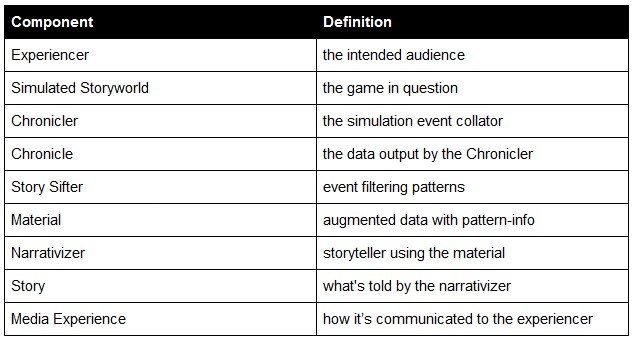
\includegraphics[width=\textwidth]{figures/4-Delve/curationist-architecture-components.jpg}
    \caption{A table of J Ryan's curationist architecture components.}
    \label{fig:curationist-architecture-components}
\end{figure}

%%%%%%%%%%%% END FIGURE %%%%%%%%%%%%%%%%%%%%%%%%%%%%%%%%

Some of these are somewhat extraneous to our purposes, but the critical components are the \textit{simulated storyworld} (the game itself), the \textit{chronicler} (the system collating and abridging game events), which outputs the \textit{chronicle} (a data object another system can operate on). What's left is a set of procedures to take on the role of \textit{story sifter} and \textit{narrativizer} to make use of the material to generate a story. Those roles are fulfilled by a prototype created in 2014 called \textit{LegendsWriter}, which operates as a component within LegendsViewer. We will return to this in more detail in Section \ref{subsubsec:legendswriter}.

\subsection{Expressionist}
\label{subsec:expressionist}

Now that we've shown some related work in simulation-driven narrativization---which covers how we acquire the \textit{chronicle}, or data object with simulation events---we can talk about how we translate that for \textit{Delve} in order to be narrativized.

This was accomplished using Expressionist, a grammar system created by J Ryan \cite{ryan2016expressionist}. Expressionist is used in several of Ryan's works, including Talk of the Town \cite{ryan2016characters} and Sheldon County \cite[p.~647-681]{ryan2018curating}. For \textit{Delve}, it was used as part of the event generation pipeline, specifically the surface text generation for character memories, and controlling how they change given player interactions.

Expressionist is an authoring system for context-free grammars \cite{bundy1984catalogue} that allow tagging on their nonterminal symbols. The tagging capability of the system puts it conceptually close to Knuth's attribute grammars \cite{knuth1968semantics}, but with the key difference that Expressionist grammars attach tags to its nonterminal symbols, not the production rules themselves.

Expressionist operates as part of a duo that together make a dynamic text generation system. Expressionist is Ryan's term for the editor that facilitates authoring, and the data structure exported from it. Productionist is a general term for the system that generates text from an Expressionist-authored grammar, and is thus called from the game’s code. Some implementations of Productionist pre-render text for different combinations of tags, so that at runtime generation becomes a lookup rather than search. While the authoring tool of Expressionist (and the data object it outputs) remain relatively the same no matter how the systems are using them, each Productionist is in practice a handcrafted, customized module that crosses that last bridge to output the necessary text, though Ryan provides an example implementation of Productionist in the public repo.

Text is generated using this system by sending a ``content request" to the Expressionist data object. This content request is composed of tags, or even hierarchies of tags, which can also be fine-tuned as ``required", ``desired" (with a simple scoring metric applied), or ``prohibited." The returned data is then processed by the custom Productionist module.

Because Productionists are custom to each implementation, they can vary widely. For example, tags on nonterminals don't necessarily have to be simple semantic strings like ``angry", ``sad", etc. They can even be code, as with Jonathan Lessard and the \textit{LabLabLab} collective's game Hammurabi \cite{lessard2017striving}. In their implementation, the ``code tags" decorating the nonterminals returned in response to queries were executed to affect the state of the game.

While not as complex as that use case, \textit{Delve} makes use of simple semantic tagging, which is later processed and translated through an ontology to new values, and then subsequently operationalized (discussed later in Section \ref{subsubsec:delve-writing-the-generative-grammars}).

This system is powerful, flexible, and expressive. But what about the combinatorics? Surely the ballooning number of combinations makes doing live queries a nightmare! This problem is solved by a third module, bundled in with Expressionist when it does its data export, called Reductionist. This module reduces the massive combinatorial space of potential grammar outputs to an optimized format that allows queries to be made quickly across the total tag combinations. It accomplishes this by ``semantically compressing" combinations to just ones with unique sets of semantic tags, bundling all the ``recipes" possible within that.

When a content request is made to the data object, the search can happen quickly to get to these groupings of recipes. And because the only text output processing is through the semantic tags, operationally it can treat any recipe it uses from that family as a valid answer to its query. The granularity of the tagging is left to the author, so if they find that certain things are returned as valid satisfactions to a tag set query that seem amiss or out of place (such as an angry reply when what was needed was an angry question) then what is required is higher definition on the tagset and tagging of the Expressionist nonterminals.

Because of Reductionist, it remains feasible to do run-time Expressionist queries for text generation despite its combinatorics, which is critical when it's used for dynamic dialogue or other instances where player interaction has changed the state space, and thus the types of tags required in queries.

\subsection{Computational Metaphor}\label{subsec:computational-metaphor}

Between simulation events and Expressionist tags, \textit{Delve} has a rich expressive state to use. But also at play with those tags is their embedding within an ontology, which is subsequently leveraged for metaphoric connections between concepts, and used to instantiate memories as physical objects, which the player can manipulate. For example, a sad memory may be tagged with the concept ``sad", which may route through the ontology to ``blue", which then grounds out in a ``blue rose" asset, which the player can interact with.

\subsubsection{Ontologies}\label{subsubsec:delve-ontologies}

When speaking of \textit{Delve}'s ontology, it's meant in its computer science context. Specifically:

\begin{quote}
    a set of representational primitives with which to model a domain of knowledge or discourse. The representational primitives are typically classes (or sets), attributes (or properties), and relationships (or relations among class members). The definitions of the representational primitives include information about their meaning and constraints on their logically consistent application. \cite{liu2009encyclopedia}
\end{quote}

%%ontologyDef%%
The core connection between \textit{Delve}'s two families of content--text memories and 3D objects--is mediated by the ontology. The core interaction of the game--manipulating the objects to change memories--relies on the players gradually understanding those connections through experimentation and play, then leveraging that knowledge to affect specific transformations. Because this desired gameplay relies on--and is driven by--the ontology, we say \textit{Delve} is an \textit{ontology-driven game}.
%%ontologyDef%%

Other games in this ontology-driven space occupy a unique intersection between the field of knowledge representation and computational media, in most cases utilizing their ontologies to procedurally generate content. While there are only a few examples, some games have successfully integrated this area of knowledge engineering into the core mechanics of their game.

\paragraph{\textit{Scribblenauts Unlimited}}\label{par:scribblenauts-unlimited}

%%%%%%%% BEGIN FIGURE %%%%%%%%%%%%%%%%%%%%%%%%%%%%%%%%%

\begin{figure}
    \centering
    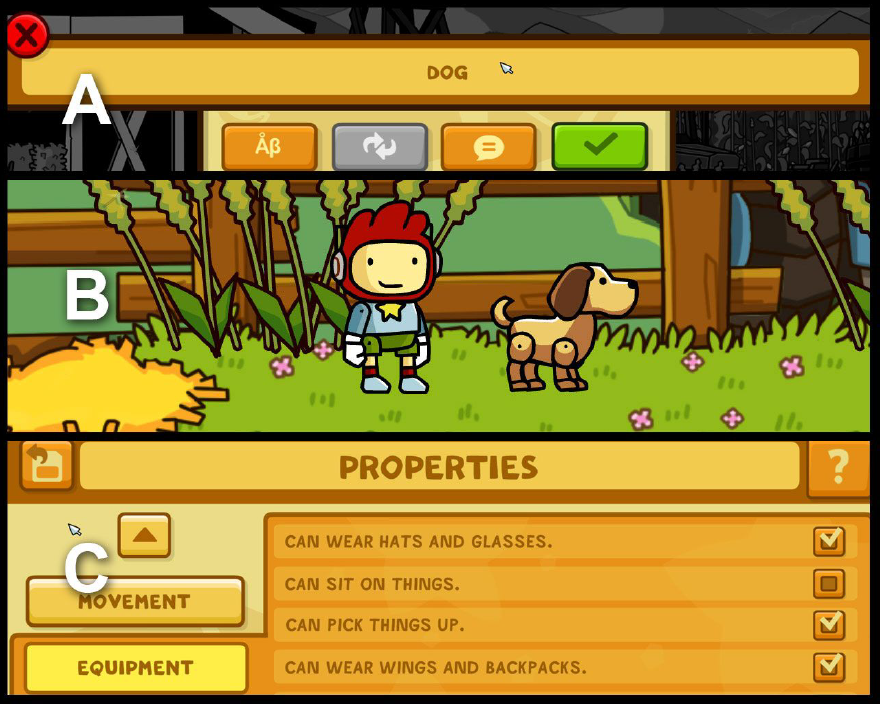
\includegraphics[width=\textwidth]{figures/4-Delve/scribblenauts.png}
    \caption{Three screen areas of \textit{Scribblenauts Unlimited}, where players type a word into their magic notepad (A) and it is instantiated in the world (B). They can also edit its properties using the Object Editor (C).}
    \label{fig:scribblenauts}
\end{figure}

%%%%%%%%%%%% END FIGURE %%%%%%%%%%%%%%%%%%%%%%%%%%%%%%%%

\textit{Scribblenauts Unlimited} is an ontology-driven game in which you solve puzzles through virtue of the main character's magic notepad. As shown in Figure  \ref{fig:scribblenauts}, the player can type in almost any word imaginable (A), and instantiate it in the game (B). The central thrust of the game is that players find emergent solutions to puzzles through the use of different objects, singly or in combination.

These objects are described in the Objectnaut database according to a schematic including ``around 40 key properties to determine an object’s behavior, including physical properties, material, electricity, temperatures, and many more attributes" \cite{tringali_2009} and are editable in the game (C in Figure \ref{fig:scribblenauts}). This database was adapted in size to be as large as possible and still fit on the target platform (Nintendo DS, iPhone, PC). At full size it has more than 10,000 unique entries.

Content is instantiated via a procedural animation system and 2D sprites. Limbs, wings, heads, and other parts each exist separately and can be modified and recombined, as can the color of each item. 

In terms of the gameplay, it's focused entirely on puzzle solving, which can only be accomplished through summoning objects or modifying objects in-game using the notepad. As a matter of fact, there are few verbs afforded to the player outside writing in the notepad, relating mostly to movement or attacking. Thus, the ability to solve puzzles is driven by an understanding of the properties of objects.

\paragraph{\textit{Argument Champion} and \textit{Dreamer of Electric Sheep}}\label{par:argument-champion}

\textit{Argument Champion} makes use of ConceptNet nodes and edges to determine valid logical connections between a starting concept and a goal concept, with the in-game purpose of convincing an audience that either your character's position on said concept is defensible and good, or that your AI opponent's position on a concept is bad \cite{smith_2012}. Harnessing ConceptNet, while notoriously problematic, lends the game an ontological model of over 1.6 million concepts and relations \cite{liu2004conceptnet}. As seen in Figure \ref{fig:dreamer-of-electric-sheep}, the words themselves are grounded out as direct printouts to the screen, contextualized as part of a speech. And the player's understanding of ConceptNet's somewhat quixotic conceptual relations directly translates to more successful arguments and a higher score.

%%%%%%%% BEGIN FIGURE %%%%%%%%%%%%%%%%%%%%%%%%%%%%%%%%%

\begin{figure}
    \centering
    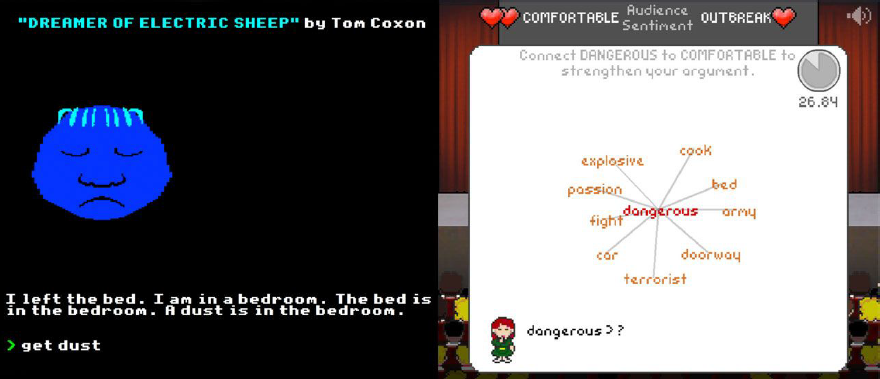
\includegraphics[width=\textwidth]{figures/4-Delve/androids-sheep.png}
    \caption{Sample output from \textit{Dreamer of Electric Sheep} (left) and \textit{Argument Champion} (right).}
    \label{fig:dreamer-of-electric-sheep}
\end{figure}

%%%%%%%%%%%% END FIGURE %%%%%%%%%%%%%%%%%%%%%%%%%%%%%%%%

\textit{Dreamer of Electric Sheep} follows a similar pattern, importing a subset of ConceptNet and then using certain connecting relations between nodes to afford actions reminiscent of interactive fiction parsers to the player (look, enter, leave, take, drop, give). Like \textit{Argument Champion}, it grounds out the representations as words on the screen that are put into sentence descriptions (Figure \ref{fig:dreamer-of-electric-sheep}). The player’s understanding of the network helps inform their actions in the game.

\paragraph{\textit{Imaginarium}}\label{par:imaginarium}

\textit{Argument Champion} and \textit{Dreamer of Electric Sheep} both make use of a very large third-party ontology (ConceptNet) and \textit{Scribblenauts} makes use of an ontology that, while hand-authored, still has over 10,000 nodes. \textit{Delve}'s ontology authoring approach, however, has more in common with approaches such as Horswill's \textit{Imaginarium} system \cite{horswill_2019}. \textit{Imaginarium} is intended as a tool for creating smaller, ad hoc ontologies for tabletop RPGs. While many ontology authoring interfaces can be complex and daunting for those unfamiliar with the space, \textit{Imaginarium}'s goal is to make that task easy enough to approach that of a casual creator \cite{compton-iccc2015}. Similarly to that, the ontology authoring in \textit{Delve} is intended to be as frictionless as possible (elaborated on in Section \ref{par:delve-implementation-the-substrate}), and authored as a way to additively connect nodes (be those Expressionist semantic tag nodes or nodes corresponding to objects and physical properties) together to facilitate the translation from memory surface text to memory palace object. However, in contrast to \textit{Imaginarium}'s interface which is evocative of natural language input, \textit{Delve} requires the user to input JSON data structures. Additionally, \textit{Imaginarium} is constraint-based, which means the data and output are guaranteed to be well-formed, whereas no such guarantees can be said about \textit{Delve}'s ontology (although that may become necessary in the future, once authoring has begun in earnest).

\subsubsection{Metaphor Systems}\label{subsubsec:metaphor-systems}

One way to drive the player to more directly engage with an ontology-driven experience is to complexify the conceptual relations, in turn requiring deeper interpretive work on the part of the player to understand. This increased engagement would (hopefully) map to increased proficiency in game tasks. In \textit{Scribblenauts} and \textit{Argument Champion} this is not the case: the instantiation of the content is a 1-to-1 correlation, the ontological frameworks largely representational, their relations descriptive of real-world qualities the objects possess. If you type ``dog" in the notepad in \textit{Scribblenauts}, it will make a cartoon version of a dog.

However, games need not be limited to literal ontologies to drive their procedural systems. There is a rich field of experiences to be created by grounding out more complex ontological relations to game assets and behaviors, and thus encourage player engagement with the underlying system.

The field of computational metaphor has insights to provide in this vein, particularly the early work of Fox Harrell and Jichen Zhu. Harrell's \textit{Alloy} and later \textit{Griot} system, and Zhu's \textit{Riu} system have been successfully used to create computational media works, grounding out their roots in semiotics and semantic theory into playable experiences.

\paragraph{\textit{Alloy} and \textit{Griot}}\label{par:alloy-and-griot}

Conceptual blending provides a methodology for combining and making connections between these frames or mental spaces, a process occurring all the time in our ``backstage cognition" \cite{fauconnier2001conceptual}.

Harrell’s \textit{Alloy} system took this conceptual blending model and translated key aspects of it into a computational model, implementing it through Goguen’s algebraic semiotics approach to blending \cite{goguen2010style}. It takes as input the data structures of the conceptual spaces and the maps between them, and outputs a diagram of a blended space, complete with mappings. A key insight here is that Harrell was not positing a sort of ground truth for these mappings as one might with symbolic AI approaches, but instead performing operations on subjective conceptual networks, which must be explicitly given to the system, pre-baked with the programmer’s preconceptions \cite{harrell_2007}.

Harrell iterated on \textit{Alloy} to create the \textit{Griot} system, which was used initially to generate his
``polymorphic poetry" works, such as \textit{The Girl With Skin of Haints and Seraphs} \cite{harrell2005shades}. This again was drawing from Goguen’s theories of algebraic semiotics to describe the sign systems involved. \textit{Griot} operated on ``theme domains", which were represented as ontologies of axiom sets relating to a specific theme. The \textit{Alloy} algorithm would then operate on those theme domains to translate between them, and then ground out the result through ``media morphisms" (which in these initial works was natural language, but in later instantiations incorporated graphics).

Additionally, Harrell also added a new type of automaton called a ``probabilistic bounded stack transition machine", or ``event structure machine" to select how the phrase templates for output were composed and arranged \cite{goguen2010style}. This sort of translation and systemization of theory-based models is very powerful, providing a way to ``ground out" the implications of the theory, to test its limits and confront its implications.

\paragraph{\textit{Riu} and Force-Dynamics}\label{par:riu-and-force-dynamics}

Zhu’s \textit{Memory, Reverie Machine} also used axioms selected from different ontologies for blending through \textit{Griot}, and applied the result to ``experiences of events, objects, and actors to affective concepts determined by current state, in this case emotional state, of the protagonist" \cite{zhu_harrell_2011}. This grounded out in the textual display of memories, which were annotated based on their subject, and retrieved through actions of the main character, the robot Ales. Zhu’s later work \textit{Remembrance} applied this approach to perform changes to the environment around the protagonist based on their current emotional state, which could result in changes from a well-lit room with cheerful music and nice furnishings to a darker room with dirtier, more bedraggled objects and more ominous music \cite{zhu2011representing}.

Another thread of work pursued by Zhu is the \textit{Riu} system, whose approach to computational analogy, specifically story representation, draws from Talmy’s theory of force-dynamics, as opposed to \textit{Griot}’s conceptual blending roots. Force-dynamics allows the formulation of graded relationships between entities, which allows more expressivity when modeling them for the purposes of story planning \cite{zhu2010story}. The particular component of this system most pertinent to \textit{Delve}'s development is \textit{Riu}’s Structure Mapping Engine (SME). 

The SME is what computes the similarity level between two ontological domains in this work, on both a surface and structural level, informed by Gentner’s structure mapping theory. \textit{Riu} uses a two-step process, starting with a surface level comparison of keywords in each content segment, and pulling out some number which have the highest level of tag overlap. Secondly, it uses structure mapping to determine on a deeper level which one of the selections provides the most similar translation into the new domain. Taking a cue from other systems, \textit{Riu} does this so that the second, computationally expensive operation is only called on a list of comparisons filtered by the shallower, yet faster, selection process.

Zhu’s later work with Ontañón pushed the idea of this mapping further through the SAM (Story Analogies through Mapping) algorithm \cite{ontanon2011sam}. SAM provides a vector for including domain knowledge in the process of generating analogous stories to the input, allowing a story with certain ontological content to be metaphorically translated across different domains.

\subsection{Summary}\label{devel-related-summary}

In summary, we've seen threads of work addressing simulationist narrativization---the practice of third-party narrative generation using data from separate systems as input, then creating narratives to enhance said systems' experiences. These works range from automated sportscasters and embedded agents in FPS games (which narrate while events happen live) to automated sports journalism systems and the use of story intention graphs to formally represent game playthroughs (narrated after play has concluded).

We then looked at Expressionist \cite{ryan2016expressionist}, J Ryan's system for semantically tagging grammars used for dynamic surface text, which is used in \textit{Delve} for character memories.

We then looked at ontology-driven games, to get a sense of related systems that have incorporated this knowledge engineering approach into their game systems. Like those, \textit{Delve} uses a simple ontology that bridges Expressionist tags with 3D game objects (which we'll explore in Section \ref{par:delve-implementation-the-substrate}). This process of computational metaphor puts it in dialogue with previous works like Harrell and Zhu's, though for our purposes our ontology is a less rigourous, and more hand-authored one.

The concept of ontology-driven gameplay through computational metaphor is one which has been with \textit{Delve} since its first conception. However, the method for how character memories are generated has gone through iteration. This iteration was mostly carried out in a previous project \textit{LegendsWriter}, while some other potential applications were explored in \textit{Argosy}. We will next briefly look at these projects, to help clarify how the event generation strategy in \textit{Delve} was solidified.

\subsection{Prior Works}\label{subsec:delve-prior-works}

\subsubsection{\textit{LegendsWriter}}\label{subsubsec:legendswriter}

As with the earlier-mentioned simulationist narrativization works, the basic premise of \textit{LegendsWriter} is that game data from a high-fidelity simulation provides a body of causally-linked, domain-constrained events as the raw material for story generation (here conceived of as narrativization). Because the generated events follow a rigorous simulation logic, the ``facts" of the stories are already baked in. We can rely on the simulation to only give us causally consistent events, not ones where, for example, the main character dies in the middle, or somehow is in two places at once, etc. The conventions of the simulation logic are the bare minimum conventions of the storytelling about that world, so they do the heavy lifting.

Note that in plan-based story generation, much of the effort of domain modeling is precisely in authoring operator preconditions and effects to correctly model the causal structure of the domain. But using the narrativization paradigm, our attention can turn to focusing on the aesthetics of narrative structures and tropes. Even though the other systems presented in this dissertation, \textit{Ice-Bound} and StoryAssembler, are not classic story planners, they too depend on the correct chaining of preconditions and effects (as well as clever state-based templating) to achieve causal coherence. \textit{LegendsWriter} gets this causal coherence for free, through virtue of the simulation it uses as input. 

The high-fidelity simulation we targeted for this was \textit{Dwarf Fortress}, and the third-party program LegendsViewer. LegendsViewer already provides simple descriptions for exported \textit{Dwarf Fortress} character events in LegendsViewer are one-line sentences, such as ``In 96, Almo confronted the night creature Ayanu Cryptmurk in the Tomb of Dusk." A selection of such a chronicle can be seen in Figure \ref{fig:legendsviewer}. When the events are read in sequence, they definitely suggest a story unique to the character involved, approaching something akin to Tale-Spin, the descriptions of sport games, or a medieval chronicle. The bones exist, but there's no meat, no leveraging of dramatic build-up. That is left as an exercise to the reader.

%%%%%%%% BEGIN FIGURE %%%%%%%%%%%%%%%%%%%%%%%%%%%%%%%%%

\begin{figure}
    \centering
    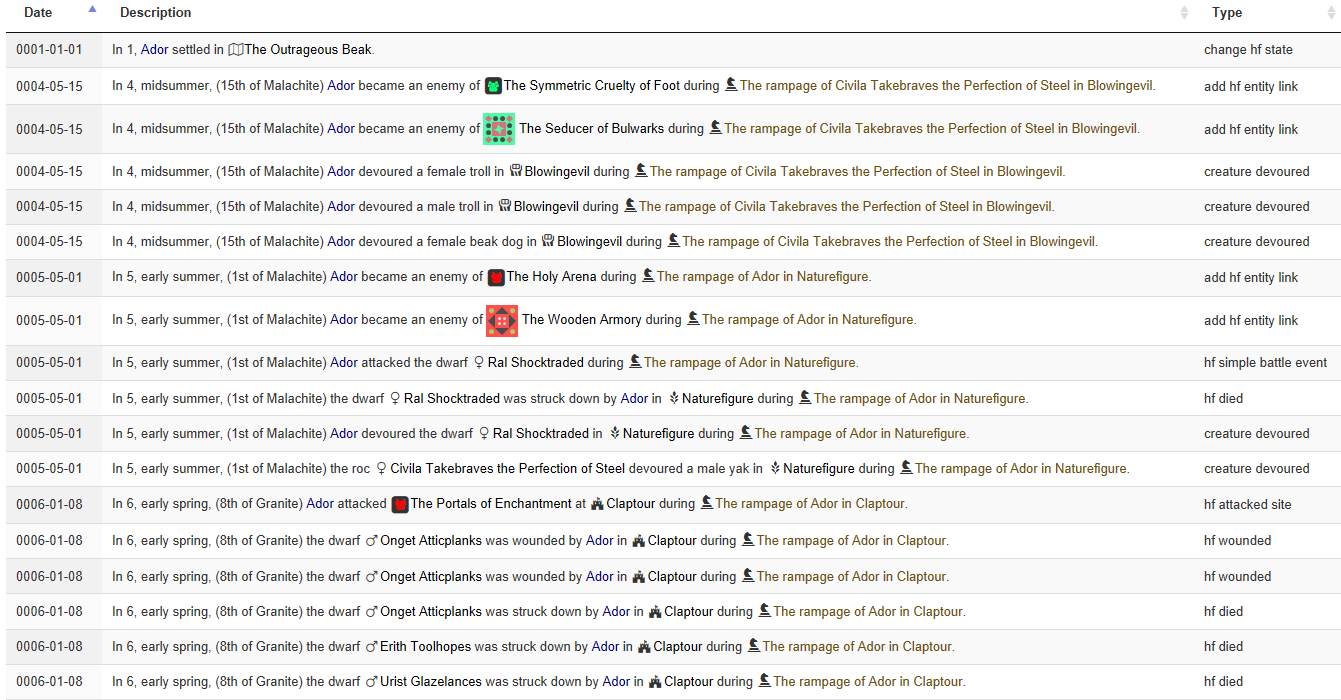
\includegraphics[width=\textwidth]{figures/4-Delve/legendsviewer.png}
    \caption{A view of character life events in LegendsViewer.}
    \label{fig:legendsviewer}
\end{figure}

%%%%%%%%%%%% END FIGURE %%%%%%%%%%%%%%%%%%%%%%%%%%%%%%%%

Thus, if we adopt the curationist architecture for this (Figure \ref{fig:curationist-legendsviewer}), we can use \textit{Dwarf Fortress} as our \textit{simulated storyworld}, the exported legends data as the \textit{chronicle} (facilitated by the third-party program DFHack) and create a new system (\textit{LegendsWriter}) to process that to create stories. The \textit{story sifting} it uses to determine which stories to tell for which characters, is something we will return to in much greater depth in Section \ref{par:sifting-patterns}, where we discuss the approach in detail for \textit{Delve} event generation. For now, we can say simply that it looks for certain sequences of events (\textit{sifting patterns}) and if matched, it runs state-driven templates to create surface text of a \textit{story} from those event sequences.

%%%%%%%% BEGIN FIGURE %%%%%%%%%%%%%%%%%%%%%%%%%%%%%%%%%

\begin{figure}
    \centering
    \includegraphics[width=\textwidth]{figures/4-Delve/curationist-legendswriter.jpg}
    \caption{A table of J Ryan's curationist architecture components, with their \textit{LegendsWriter} corollaries.}
    \label{fig:curationist-legendsviewer}
\end{figure}

%%%%%%%%%%%% END FIGURE %%%%%%%%%%%%%%%%%%%%%%%%%%%%%%%%

Though \textit{Dwarf Fortress} allows us to circumvent the ``causal coherence" problem, it presents a potentially even greater challenge of its own in the high resolution of its simulation. Character life stories can have anywhere from a handful to thousands of life events. Each one of these life events can be in one of 62 different categories (see Figure \ref{fig:DF-event-types}). Furthermore, each category may contain sub-categories, such as with ``hf change state." Depending on the state change, that category can encapsulate a character settling down in a new town, scouting locally for trouble, becoming a thief, hunting for food, becoming a kidnapper, or any combination thereof.

%%%%%%%% BEGIN FIGURE %%%%%%%%%%%%%%%%%%%%%%%%%%%%%%%%%

\begin{figure}
    \centering
    \includegraphics[width=\textwidth]{figures/4-Delve/dwarf-fortress-event-types.jpg}
    \caption{Different life event categorizations. ``HF" here means ``historical figure", a civilization or individual who has accumulated enough life events to merit recording in the Legends XML chronicle.}
    \label{fig:DF-event-types}
\end{figure}

%%%%%%%%%%%% END FIGURE %%%%%%%%%%%%%%%%%%%%%%%%%%%%%%%%

However, we don't need to solve all of \textit{Dwarf Fortress} to create interesting stories. We can start by covering subsets of event types as selected by a user.  Because LegendsViewer is available as an open source project, it was possible to modify its code directly, such that character events we pull out to narrativize are given a ``storyedness" amount. This amount can be determined by the author while writing---for example if they want to take significant time to build out a particularly elaborate story, they can give character events involved in it a ``storyedness" rating of 5. Smaller stories can be 1, and so on. These events can them be summed up per-actor, to give each actor a total ``storyedness" amount.

We can then add ``storyedness" as a filter to LegendsViewer's UI, which is already capable of navigating between characters. By adding an additional ``storyedness sort field" to the LegendsViewer interface, we gain the ability to pluck out only characters that possess rendered stories that we've authored content for. This approach means content can be authored incrementally, and we can see the exemplar stories by leveraging the existing LegendsViewer interface. Essentially, we gain event generation from \textit{Dwarf Fortress} ``for free", and leverage an existing well-developed project that allows us to sensibly navigate and filter the dataset. All that's needed now is to author the patterns.

\paragraph{\textit{LegendsWriter} Pattern Authoring}\label{par:legendswriter-pattern-authoring}

As can be seen in Figure \ref{fig:legendswriter-output}, these experiments with handcrafting story sifters centered around night creatures (vampires), a specific subset of \textit{Dwarf Fortress} characters. These were chosen as an initial focus for two reasons. One, such characters reliably have at least one sequence of events with three specific categories: ``hf gains secret goal: immortality", ``hf profaned structure", ``hf does interaction: deity curse." In \textit{Dwarf Fortress}, one becomes a vampire after desecrating a sacred site, and being cursed by a deity. This naturally lets us create a sifting pattern ``storyOfImmortality", composed of those three event categories. The second reason is that night creatures are immortal. Unless meeting a grisly end, their lives typically contain several hundred events. This gives us a wider variety of events to filter, thus increasing the chances that our patterns match. This makes the bar for catching things in our sifting patterns very low, which is good for exploratory prototyping.

% \begin{quote}
%     In the year \textbf{121}, \textbf{as summer withered into fall}, trouble found \textbf{\underline{Rakust}}. It was in \textbf{\underline{Painttarget}}, where members of \textbf{\underline{The Humid Lance}} accused \textbf{\underline{Rakust}} of \textbf{murdering a local}. \textbf{Ironically,} \textbf{\underline{Rakust}} \textbf{had not murdered anyone...in \textbf{\underline{Painttarget}}, at least. Her} accuser stepped forward and \textbf{laughed unpleasantly. ``To kill is a terrible crime."} \\
% \textbf{\underline{Rakust} flicked her eyes} to the \textbf{grumbling} crowd. \textbf{``What is that supposed to mean to me?"} \\
% \textbf{After muttered imprecations}, the \textbf{locals dissipated}. \\
% After that, \textbf{\underline{Rakust}} decided discretion was needed, and so left \textbf{\underline{Painttarget}} to settle in \textbf{\underline{Championgirders}}. \\
% For \textbf{a while things were quiet, but once again \underline{Rakust}'s past, or at least reputation, would come back to haunt them}. This was \textbf{four} years later, \textbf{in spring, when the crocuses had just sprouted}. Everything had been uneventful since she'd re-settled in \textbf{\underline{Championgirders}}. \\
% Then one day, there was a knock at the door. \textbf{\underline{Rakust}} opened it, to reveal \textbf{most of \underline{The Fortification of Truth}}, who immediately accused her of \textbf{murdering some nobody}. Ironically, \textbf{\underline{Rakust} had not murdered anyone...in \underline{Championgirders}, at least. Her} accuser stepped forward and \textbf{glowered. ``We don't take kindly to murderers here."} \\
% \textbf{\underline{Rakust} swallowed carefully. ``I'm sure I don't know what you're talking about."} \\
% After \textbf{a few minutes of hot silence, the mob dispersed}.
% After that, \textbf{Rakust} decided discretion was needed, and so left \textbf{Championgirders} to settle in \textbf{Foggyrims}.
% \end{quote}
%%%%%%%% BEGIN FIGURE %%%%%%%%%%%%%%%%%%%%%%%%%%%%%%%%%

\begin{figure}
    \centering
    \includegraphics[width=\textwidth]{figures/4-Delve/legendswriter-output.jpg}
    \caption{Example \textit{LegendsWriter} output. Bold words are dynamic. Underlined words are simulation entity references.}
    \label{fig:legendswriter-output}
\end{figure}

%%%%%%%%%%%% END FIGURE %%%%%%%%%%%%%%%%%%%%%%%%%%%%%%%%

\paragraph{Procedural Subjectivity}\label{par:procedural-subjectivity}

This approach could also facilitate the creation of a system where there is a subjective notion of history, and those notions can be unique to different character perspectives, as we saw adapted with the sports commentators in Rocco and Byrne \cite{andre2000three}. Originally, \textit{LegendsWriter} was titled ``Dwarf Grandpa", because the idea was that simple filtering metadata could be added to the sifting patterns, such that a ``farmer grandpa" or ``battle-worn grandpa" etc would have different sifting pattern pre-conditions, and thus yield different stories from the same set of events.

The combination of hierarchical nesting along with ``role-based narrator" preconditions on sifting patterns could be an incredibly powerful design pattern to use in dynamic narratives. While it remains the domain of future work, one can easily imagine a set of global patterns that can be applied, then culture-specific patterns nested beneath that, then character-specific patterns, then state-specific patterns. For example, a character could relate a story who reads lots of romances. If one wrote many patterns with ``romance" tags, then when you have a player ask them to describe a brooding, aloof character, they may come up with a very different interpretation of said character’s history than if you asked someone who hates people that brood. None of the actual motivations or things referenced in the event text need necessarily be modeled in the simulation, so long as they’re consistent to the narrator.

This technique could be potentially used to create conflicting accounts that, critically, conflict in consistent ways. You could have two characters witness a murder, one who’s a pessimist, and another who believes in justice in the hereafter. When asked to describe the event, the pessimist would consult their library of patterns, output the text ``Someone was murdered–which just goes to show that life is short and brutal." and you could surface why to the player with something like ``(Char1 is a pessimist)." The other character would have access to patterns that would render text ``Someone was murdered–but the murderer will get what’s coming to them, in life or the hereafter" with the explanation ``(Char2 believes in justice in the hereafter)." Again, the power of this approach depends wholly on the sifting pattern library and narrativizer, which can be gated on groupings of characters on culture, socio-economic status, disposition, or even dynamic tags that happen as a result of the simulation, like ``survived trauma" or ``wonderful childhood." 

While only a preliminary amount of authoring was done with \textit{LegendsWriter}, it did provide fertile initial ground for exploring the technique of story sifting, and generating stories from particular sequences of simulated events. The techniques explored for this could be broadly categorized as ``top-down" and ``bottom-up", which will be covered in Section \ref{par:sifting-patterns}.

However, these patterns were matched automatically by the system, and getting to acceptable levels of ``event coverage", where many of the simulated events were able to be encapsulated by these patterns, proved very difficult. Getting to the point where readers could get an appreciable amount of interesting and diverse stories from \textit{Dwarf Fortress} events would take a lot of authoring. This prompted a different design approach for a later prototype, \textit{Argosy}.

\subsubsection{\textit{Argosy} and Sculptural Sifting}\label{subsubsec:argosy-and-sculptural-sifting}

In \textit{LegendsWriter} the application of sifting patterns was automatic, controlled by the heuristics and pre-conditions added to them when they were authored. As such, it isn't interactive, though it is generative.

In order to explore how sifting patterns can be shifted from a post-generation process to a core part of a game's mechanics, controlled by the player, a prototype game called \textit{Argosy} was created. 

The narrative framing is that you're an occultist who has been unexpectedly put in charge of a secret government lab of scientists, after your predecessor went mad. The scientists are working on a weapon to close eldritch portals, which have unexpectedly started opening all over the world. 

%%%%%%%% BEGIN FIGURE %%%%%%%%%%%%%%%%%%%%%%%%%%%%%%%%%

\begin{figure}
    \centering
    \includegraphics[width=\textwidth]{figures/4-Delve/argosy.png}
    \caption{Screenshot of \textit{Argosy}.}
    \label{fig:argosy}
\end{figure}

%%%%%%%%%%%% END FIGURE %%%%%%%%%%%%%%%%%%%%%%%%%%%%%%%%

At the end of each turn, each member of your team takes sanity damage from the number of ``unexplained events" on their timeline. As the leader and an accomplished occultist, you have access to ``supernatural schemas" which you can use to ``explain" a certain number of events, by allocating the schema to them. Your goal is for your team to survive a certain number of turns without going mad, so they can close the portals.

Mechanics-wise, each team member has their own timeline of events. Each event is one of five different types. At the end of your turn, each scientist takes ``unexplained event" sanity damage. If their sanity falls to zero, then they are removed from the game. If they survive, five new events are added to their timeline

Each turn you are granted some number of schemas (the in-game term for sifting patterns) which each have three ``anchors." The anchors' colors correspond to the event types. The player drags these anchors onto events matching that color on any of their scientists' timelines. When they do, the anchor connects to that event. When the player matches all three anchors to the timeline, the span of events covered by the schema are then ``explained." A simple heuristic is used for calculating the ``amount of explanation" that it affords, a linear falloff based on distance from the anchors. This prevents players from using a schema to simply cover an entire character's timeline from beginning to end.

As with \textit{Ice-Bound}, this game shows promise because of its systemic framing that sidesteps some of the pernicious authoring problems for combinatoric narratives. By framing the explanation of events with the schemas as a goal, we shift the player's role from generative narrative critic to constructive collaborator. System shortcomings (such as a lack of schemas that can adequately cover timeline events) are cast instead as deliberate designs for challenge, rather than an authoring failure.

\paragraph{Surface Text}\label{par:argosy-surface-text}

Because the usual concerns of how to accomplish coverage of events through story sifting patterns is set aside as a game mechanic, our main focus for this prototype is the surface text for events, and the explanations generated by putting schema anchors on events. The ``narrativizer" for \textit{Argosy} works through a combination of simple context-free grammars (using Compton's \textit{Tracery} library \cite{compton2015tracery}) synced between the event and the schema anchor. For example, an event might have the description ``The statues in Times Square started speaking in blood." after running the grammars in Figure \ref{fig:argosy-event-data} (in the field ``description"). A schema with an initial tag of ``omens" (like the one in Figure \ref{fig:argosy-event-data}) could put the first anchor on this event. When doing so, the hook in the event is populated to the schema, such that the ``explanation" field's first entry reads ``The statues are conduits for eldritch energies." If the anchor is switched to a different ``omens" event, it will likewise update.

%%%%%%%% BEGIN FIGURE %%%%%%%%%%%%%%%%%%%%%%%%%%%%%%%%%

\begin{figure}
    \centering
    \includegraphics[width=\textwidth]{figures/4-Delve/argosy-event-data-object.png}
    \caption{\textit{Argosy} event data object, containing a ``hook" that is set in the ``description" that is used by anchors in schemas.}
    \label{fig:argosy-event-data}
\end{figure}

%%%%%%%%%%%% END FIGURE %%%%%%%%%%%%%%%%%%%%%%%%%%%%%%%%

%%%%%%%% BEGIN FIGURE %%%%%%%%%%%%%%%%%%%%%%%%%%%%%%%%%

\begin{figure}
    \centering
    \includegraphics[width=\textwidth]{figures/4-Delve/argosy-schema.png}
    \caption{Data object for an \textit{Argosy} schema. The \_anchor1:hook1\_ syntax allows the explanation text to change depending on which event the anchor is attached to.}
    \label{fig:argosy-data-schema}
\end{figure}

%%%%%%%%%%%% END FIGURE %%%%%%%%%%%%%%%%%%%%%%%%%%%%%%%%

These schemas also have metadata, in the form of the ``traits" field, which are applied to scientists when a schema is applied to their timeline. These are simple flags which can be set as preconditions for further schemas. Therefore, using schemas on characters changes the characters, which can potentially impact which explanations are valid for them in the future, or perhaps even more game processes tied to different mechanics.

While only a prototype for now, this game design shows there are substantial ways that story sifting can be adapted to not only provide generative text for events that have already happened, but put the player ``in the loop" and expose part of the process as core game mechanics, and thus also avoiding some potential authoring pitfalls.

\subsubsection{Prior Works Summary}\label{subsubsec:delve-prior-works-summary}

These two experiences represent generative narrative internally, as well as externally through third-party programs. This allowed us to demonstrate two prototypes that leveraged ``curationist architecture" to tackle narrative generation in dialogue with the simulation systems. In the course of this we were able to explore authoring approaches for sifting patterns, which we'll return to in \textit{Delve} in the following section.

Bringing both Related and Prior Works together, we're now sufficiently positioned to talk about \textit{Delve}, an exploratory system that pre-generates history for its characters, in service of constructing a chronology of memories for each one. Those memories are instantiated in a 3D space (a ``memory palace") as user-manipulable objects. When the objects are changed, those changes then map back to the memories, changing the data representation, as well as the surface text.

\section{System Description}\label{sec:delve-system-description}

\textit{Delve}'s general architecture centers on the creation of a character "memory", which consists of a data object capable of generating text (marked up with references to accompanying 3D objects), given a set of requested semantic tags. Both the event generation system and the systems that enabled the manipulation of memories make this significantly more complicated than either\textit{ Ice-Bound} or StoryAssembler works by a wide margin. Furthermore, the authoring challenge these compounded combinatorics, constrained by the hierarchical event generation, pose is not one that's been fully grappled with yet. Because work is ongoing on the finer points of the system as well as non-prototype content, we'll talk about the current implementation details, as well as likely changes based on existing authoring experience with the system. In terms of Authorability, we'll discuss how applying analysis through the lens of its sub-categories informed where to spend authorial effort.

\subsubsection{Description of the System}\label{subsubsec:delve-description}

%%%%%%%% BEGIN FIGURE %%%%%%%%%%%%%%%%%%%%%%%%%%%%%%%%%

\begin{figure}
    \centering
    \includegraphics[width=\textwidth]{figures/4-Delve/delve-diagram.png}
    \caption{Flow between different systems in \textit{Delve}, moving from simulation timesteps to generation of a memory palace artifact from a character event.}
    \label{fig:delve-diagram}
\end{figure}

%%%%%%%%%%%% END FIGURE %%%%%%%%%%%%%%%%%%%%%%%%%%%%%%%%

%%GDoc comments%%
While refinement of core \textit{Delve} architectures is ongoing, the basic flow between its systems can be seen in Figure \ref{fig:delve-diagram}. The execution is as follows: when \textit{Delve} starts, it simulates events to fill some preset amount of ``timesteps." For each timestep, it goes through an ordered list of characters sorted by ``narrative power" (a simple metric set when they are generated) and pulls a valid event from the event library to cast them into. Event validity involves checking a precondition against the current simulation state. Once chosen, the effects for that event are run, modifying the simulation state. The event is then passed to the ``surface text realization" system. The Expressionist grammar is then run for that memory, and the memory text is stored. The semantic tags resulting from that output are sent to the ontology system (called the Substrate), which finds a valid connected concept node corresponding to a physical objects. Then, both the memory text and concept nodes are sent to the Memory Palace Artifact Library, which instantiates the 3D object in the scene, along with the object transformations that can be applied to it. These object transformations are paired with their corresponding text transformations, such that the system can modify the text of the memory to match the object state, if the player changes it.
%%GDoc comments%%
Once the simulation of all characters' histories is complete, the player can then ``delve" a character, which displays the rooms of their memory palace, with the memory objects instantiated. The player can then select objects and read the corresponding memory. They can also change the object in certain ways---such as transmuting the material or moving it---which in turn affects the memory text.

\subsection{Core Architectures}\label{subsec:delve-core-architectures}

\subsubsection{Land and Prop Generation}\label{subsubsec:land-and-prop-generation}

Before the player can navigate character memory palaces, the characters need memories. And in order for characters to have memories, they need some model of location where those memories take place. So we need to generate some areas.

Because the main focus of \textit{Delve} is on the complex mapping of possibility space to surface text generation for memories, the underlying simulation is of less initial importance (though for future work this is obviously a rich area to increase generativity of the system). As such, the land generation is kept as simple as possible. Land is divided up into ``areas", which have a type, such as ``forest", ``mountain", or ``plains." Each area is also populated by props, which are treated by the system as---and have similar properties to---characters. The key difference is mostly an authoring convention in that they lack volition (i.e., they can't initiate events, and are not required to have every timestep fulfilled). However, the system supports casting them into events, such that---for example---a specific prized possession can be stolen from one character by another. This architecture choice also means that once the history has been generated, objects can be potentially queried to see what their ``story" is.

Each area is connected to at least one other area, and then further connections are layered in. These connections are labeled as ``leylines", because---unlike traditional physically-based roads or paths---area connections are intended to be mutable and non-physical, relying more on the changing of their inhabitants or game state to determine which are connected and which not. This also avoids getting bogged down in topological map generation code, as that is a solved problem outside the main concern of the project.

The main capability this adds is the ability of characters to move to other locations, and initiate events with other characters that are in the same area as them. It also populates areas with concept nodes that tie to the ontology (e.g. forest, mountain, plains, etc) which can be leveraged if necessary as hooks for later additions to the generative systems.

\subsubsection{Character Generation}\label{subsubsec:delve-character-generation}

Initial character generation is still a somewhat nascent system in \textit{Delve}, but there are two pertinent characteristics which touch the other systems, and are designed to have an integrated impact on the initial history generation.

\paragraph{Domains and Dominions}\label{par:domains-and-dominions}

Characters start out with an initial domain in which they possess a small integer amount of influence. These domains are flagged entities in the ontology, which connects the event generation and memory object / palace system. Domains are concepts like ``fire" or ``iron" or ``laughter." If a character has the most points in a given domain, they are said to be the ``Dominion" of that concept. When any events happen with output text containing semantic tags relating to a domain, the associated Dominion accrues some amount of ``favor" from the characters participating in the event. 

While purely a design convention, in practice this is meant to facilitate stories where Dominions become more and more powerful, until they ``call in their favor" with another character, usually to their benefit. Other events can be triggered whose effects lower a particular character's domain score, thus producing a give-and-take dynamic.

Eventually, this system is meant to provide the backbone for the game's main player interaction. The manipulation of memories results in different semantic tags being active for said memories, which can then result in a given character losing or gaining their Dominion. Characters approach the player with ``quests" to find a particular character, delve their memories, and change them correctly to correspond to desired domains.

\paragraph{Relationships}\label{par:delve-relationships}

Characters also start with an initial relationship with another character, to facilitate events which might have a relationship casting requirement. Most of the planned events in \textit{Delve} require more than one character, and who is cast into the supporting character role will often be driven by relationships.

Relationships in \textit{Delve} have an associated concept node and a strength between 0 and 1. This means that a relationship isn't limited to the typical fare of friendship, love, or hatred. This is intended to capture more nuanced and specific relationships, such as someone who buys bread every day from a baker developing a “bread” relationship with the baker. Relationships can also be between characters or props. This allows a character to, for example, have a relationship with their sword with the concept ``murder." This is intended to provide more hooks for event casting to latch onto, and provide more interesting granularity between characters as the history generation plays out. For example, one might imagine a character who is the Dominion of ``revenge" setting the player a quest to change another character's relationship with their favorite sword such that the associated concept is ``revenge", so that the Dominion can demand it be given to them.

\subsubsection{Event Generation}\label{subsubsec:event-generation}

With this simple layout of lands accomplished, and some initially seeded characters, we can now talk about event simulation. We knew the strategy ultimately selected for event generation and narrativization would be one of the key underpinnings of \textit{Delve}, and greatly impact both the character of the system, and thus the authorial leverage of content authoring for it. Therefore, much time was given to exploring the ramification of different approaches. Specifically, these different approaches are for the application of \textit{sifting patterns}, which we will first define and cover in detail. We will then cover the two broad categories of approach: bottom-up (which was ultimately abandoned) and top-down (which was ultimately chosen). Once we've established that, we can then broadly talk about the generation procedures (beginning with Section \ref{par:delve-generation-procedure}).

\paragraph{Sifting Patterns}\label{par:sifting-patterns}

As mentioned in earlier sections, \textit{sifting patterns} is a term coined by J Ryan as part of his curationist architecture \cite[p.~249-250]{ryan2018curating}. It specifies a pattern---be that regular expression or otherwise---used to filter raw sequences of events, such as from a chronicle export of a simulation. The \textit{sifting pattern} draws out the events for a story, and the \textit{sifting heuristic} scores those sets, or guides the initial pattern. These heuristics can be simple or complex, depending on whether creators want to spend focus on the initial sifting as the point of refinement, or on subsequent processes (such as state-driven templating or grammars) to refine the output from rougher-grained sifting once that occurs.

Sifting patterns can be wholly automated, authored and executed with no input from the player, as we saw with \textit{LegendsWriter} in Section \ref{subsubsec:legendswriter}. They can also exist in dialogue with players, such as with the \textit{Argosy} prototype in Section \ref{subsubsec:argosy-and-sculptural-sifting}, or Kreminski et al's system \textit{Felt}, which ``assists players in the process of narrativizing their play experiences by helping them locate sites of potential narrative interest in a larger simulated storyworld" \cite{kreminski2019felt}.

In a way, sifting patterns can also be thought of as siblings of playtraces, which in some cases are pattern specifications run over sequences of game events seeking to find matches. Playtracing in general has a rich field of research associated with it. A good exemplar that strongly relates to sifting is Osborn's Playspecs \cite{osborn2015playspecs}. Playspecs provides a regular expression framework for finding patterns in large sequences of player actions or game events. The tracking of events or sequences is configurable and customized to the game it's used on. The system is capable of processing playtraces composed of thousands of events, such as tracking button presses in a level playthrough of the classic platformer \textit{Super Mario Brothers}.

This work was later further developed by Osborn to also provide a method to calculate and display the edit distance between traces via similarity metrics \cite{osborn2014evaluating}. These similarity metrics were also customized on a per-game basis. Specifically, this technique was applied to \textit{Prom Week} \cite{mccoy2012prom} to see how well the system’s similarity criteria could match the \textit{Prom Week} developers’ implicit notion of playtrace similarity. This matches the domain of application, as Osborn saw Playspecs--and by extension the Gamalyzer system--as a productivity enhancer for game designers, helping them profile the levels they create in systemic ways.

However, because each scene in \textit{Prom Week} is framed like a scene in a story (``Zac tries to win over Chloe", etc) individual playtraces can bear a remarkable similarity to Legends Mode in \textit{Dwarf Fortress}---a chronicle of actions taken by simulation agents towards a particular goal. It remains work for a future researcher, but it appears to be a straightforward application to adapt the Playspec methodologies to instead map (dis)similarity between character lives in \textit{Dwarf Fortress} or similar games. Instead of playthroughs, we would have sequences of events comprising characters' lives. By carefully delineating similarity metrics, we could not only find stories which match pre-determined patterns, but ones which come close, yet deviate in particular ways. The ``edit distance" in this sense would be stories which are ``close" to our sifting pattern, but not quite matching. This could yield a potentially rich arrangement of story families, giving us more what Grinblat terms a ``story volume" \cite{grinblat2017emergent} than a single story.

As we can see, sifting patterns are a powerful strategy for generating stories from large collections of simulation events. But how we deploy them---the patterns we choose, and how those potentially nest---can result in radically different authoring strategies. Two broad strategies were explored when authoring the sifting patterns, which yielded two different results: ``top-down" and ``bottom-up."

\subparagraph{Bottom-Up}\label{subpar:delve-bottom-up}

The bottom-up approach focuses on individual events or pairs of events. In general, we want to write bottom-up content with an emphasis on contextuality and flexibility, as well as variation upon repetition. An output of such a two-event pattern for \textit{LegendsWriter}---about a vampire coming under suspicion of murder and being forced to re-locate---was given in Figure \ref{fig:legendswriter-output}. That particular example outputs different text if run multiple times for the same character (Figure \ref{fig:legendswriter-output} shows it being run twice consecutively). Additionally, if this particular example is called more than four times for one character without interstitial events, it lumps all the other matching instances into a generalized output, in order to avoid repetitive story segment generation. A selection from one instantiation of that pattern (confrontAndMove) is provided in Figure \ref{fig:legendswriter-diagram}, with each event flag labeled.

%%%%%%%% BEGIN FIGURE %%%%%%%%%%%%%%%%%%%%%%%%%%%%%%%%%

\begin{figure}
    \centering
    \includegraphics[width=\textwidth]{figures/4-Delve/legendswriter-diagram.png}
    \caption{Sample output from a ``bottom-up" pattern for \textit{LegendsWriter}, matching a pattern for two consecutive two events: ``hf confronted" and ``change hf state." Bold text is dynamic, underlined text denotes simulation-specific references.}
    \label{fig:legendswriter-diagram}
\end{figure}

%%%%%%%%%%%% END FIGURE %%%%%%%%%%%%%%%%%%%%%%%%%%%%%%%%

Bottom-up approaches have a higher likelihood of matching to more total events in general, as they are more granular. Similarly, this approach is more well-suited for narrativization that requires us to increment and consider events ``live", or one tick at a time, as it supports matching on only one or two events as they're added. However, its granularity also means there is a greater potential for more unforeseen juxtapositions, and bridging between those instantiations is difficult. 

Additionally, in order to apply the bottom-up approach to \textit{Delve}, we would need either a very diverse set of simulation events (which it was felt would divert too much time that could be better spent on the narrativization itself) or to author dynamic enough single-event instantiations that the output wouldn't be repetitious. It was concluded that doing that authoring work to react to context might be better served instead using the top-down approach, which as we'll see in the next section, allows more context to be layered in.

However, we will revisit the bottom-up approach in future work for \textit{Delve}, when we tackle time ticking forward as the player plays the game, creating more memories for characters. Doing so will require either adapting the top-down events in some way to fit the "live" constraints of event generation, or possibly a completely differently-designed class of events to fit the bottom-up approach. Again, to emphasize: the difference between these two approaches is not procedural or apparent on the code level, but rather wholly contained within the design of the content used by the system. The capabilities of the authoring system can facilitate either strategy.

\subparagraph{Top-Down}\label{subpar:delve-top-down}

Another story-sifting approach involves specifying longer event sequences to match. These top-down sifting patterns may contain several events in sequence to be matched, with potentially some number of allowed events in-between.

Consider a sifting pattern that covers 50 events, and also establishes some parameters or bindings for those 50 events (such as a protagonist character). When we recursively run this process for smaller groups of events within those 50, we can pass those parameters in, further contextualizing the output of those grammars. And if those patterns have matching sequences that are, say, 10 events long, when we drill down into sifting patterns that are even smaller, we pass down both the parameters from the 50-event sifting pattern, and the 10-event sifting pattern. This way, we preserve coherency in the story's structure, and can also enrich on a very granular level the per-event sifting pattern. For example, just because a character feels shy at a party, doesn't mean they have to feel shy at all subsequent parties in their life. Therefore, what we want is \textit{local consistency} and \textit{global variance}. Figure \ref{fig:legendswriter-output-tiquo} provides an example of the output from such a top-down sifting pattern in \textit{LegendsWriter}.


% \begin{quote}
%     \textbf{Tiquo}'s terrible obsession began in \textbf{71, when shadows were long and the sun red}. \textbf{He} resolved that \textbf{he} would not succumb to old age, but instead would discover the secret of immortality no matter the cost. \\
% \textbf{After mere months}, \textbf{Tiquo} found what he sought. All other avenues had been exhausted. The only remaining option was \textbf{desecration}. The temple at \textbf{Fruitthroats} was where, with reckless abandon, \textbf{Tiquo drove the priests screaming from the sanctuary and fouled the sacrament}. \\
% But \textbf{Tiquo's} actions had not gone unnoticed. The \textbf{Sunfish god Aco, arbiter of coasts, whose terrible form is worshiped by The Nation of Scribing}, had witnessed the deliberate destruction of his most holy place, and thus \textbf{enraged}, cursed \textbf{Tiquo} to the horrific form of \textbf{vampire, doomed to eternally thirst for blood}. But \textbf{Aco's} fury was \textbf{Tiquo's} gain, for \textbf{he} had seized an immortality, even though monstrous, for his own.
% \label{fig:top-down-sifting-example}
% \end{quote}
%%%%%%%% BEGIN FIGURE %%%%%%%%%%%%%%%%%%%%%%%%%%%%%%%%%

\begin{figure}
    \centering
    \includegraphics[width=\textwidth]{figures/4-Delve/legendswriter-output-tiquo.jpg}
    \caption{Example output from a sifting pattern with top-down approach. Bold text is dynamic.}
    \label{fig:legendswriter-output-tiquo}
\end{figure}

%%%%%%%%%%%% END FIGURE %%%%%%%%%%%%%%%%%%%%%%%%%%%%%%%%

The top-down strategy has its limitations too, however. This is because, if we used it for a simulation ticking forward in a ``live" manner, we may pre-suppose a commitment to a future event in order to match a top-level ``large time period" event, which may be invalidated by a set of effects or generated event before the pattern is matched. Put another way, it could mean that at any given point we may have one or several sifting patterns determining what a character's future holds (in an earlier \textit{Delve} prototype this was called a character’s \textit{geas} or \textit{fate}).

These issues occur from the ``liveness" of the simulation, but also because the procedures of the simulation can potentially be in conflict with the procedures of the narrativization. The top-down approach works best when the only mechanics that can influence the simulation occur within the event library. Essentially, if there are state changes that can occur that aren't accounted for by the event library, then there's a chance the game can transition to an invalid state that it can't recover from. This is because the rules governing the player's interactions may not match up exactly with the event logic's ``rules", which are mostly hand-authored and are coherent more through design convention than procedural enforcement.

For \textit{Delve}, we're not dealing with live simulation. Rather, our use-case is the initial pre-populated character histories which we want to represent as objects. For that, the desired quality for our narrativization is coherence over coverage. We want more control over multi-event character arcs---arcs driven by story logics and design more than the granularity and expressiveness of the simulation. For these reasons, we opted for the ``top-down" approach, providing its nesting context, which in turn helps control character casting and allows other references to persist across events.

To illustrate this control, imagine a collection of events encapsulating one character throwing parties and inviting other characters, then accruing favors from those friends, and finally calling in those favors later on. The difference between top-down and the bottom-up is that the top-down events can more easily enforce collections of shorter events, as shown in Figure \ref{fig:two-strategies}.

%%%%%%%% BEGIN FIGURE %%%%%%%%%%%%%%%%%%%%%%%%%%%%%%%%%

\begin{figure}
    \centering
    \includegraphics[width=\textwidth]{figures/4-Delve/two-strategies.png}
    \caption{Top-down approach with hierarchical scaffolds, versus bottom-up, where events are evaluated individually for pre-conditions, and surprising juxtapositions may occur, unless highly-specific preconditions are written to manually chain events.}
    \label{fig:two-strategies}
\end{figure}

%%%%%%%%%%%% END FIGURE %%%%%%%%%%%%%%%%%%%%%%%%%%%%%%%%

In contrast, in practice it would be more difficult to ensure that such specific arrangements of events happen if we generate events one at a time, then try to apply a pattern onto them. Of course one could enforce that by writing pre-condition terms to that effect, but the number of required pre-condition terms to accomplish that makes it infeasible once the number of events grows larger, and putting that number of terms on each event reduces authorial Clarity, as opposed to simply adapting a top-down approach.

\subparagraph{A Note on Hybrid Approaches}\label{subpar:a-note-on-hybrid-approaches}

Top-down approaches are good for pulling out interesting arrays of life events, and giving an over-arching shape to the character's whole life. However, given their longer sequences and higher specificity, they don’t show up for a wide variety of character lives. For example, in LegendsViewer the sifting pattern in Figure \ref{fig:legendswriter-output-tiquo} is only triggered around thirty times for a world populated by thousands of characters, containing hundreds of thousands of events. Additionally, those stories tend to look fairly similar, and so much effort must be spent to increase their surface text generativity.
 
Bottom-up grammars are good for diffusing more rendered text amongst characters. However, they require far more labor to create, given that in order to avoid sounding repetitive, they require more dynamic input. This can be solved partly with random variation of descriptions, such as the confrontation text in Figure \ref{fig:legendswriter-output}, but to truly leverage the strengths of the system it would be better if grammars vary based on parameters that are passed down to them by top-down sifting patterns. Alternatively, grammars can be made for periods of interstitial time between flags (which may contain an arbitrary number of events) which key off the highest frequency of particular events, and then output short sentences along the lines of ``the next [n] years were filled primarily with [battles], until..." The union of these two approaches is where one could potentially see both wide coverage of events, and well-formed stories emerge, though this remains in the domain of future work.

\paragraph{Generation Procedure}\label{par:delve-generation-procedure}

\textit{Delve} uses the top-down approach for these reasons, and also because simulation is not as important to the immediate research goals as generating fully fledged, rich event descriptions and evaluating the authorial burden of that. The hope is to slowly turn the dial up on the expressivity and generativity of the history generation by building out pre-conditions and effects of the events. But the most centrally important thing is the memories themselves–specifically, the semantic tags associated with them, and the breadth of generativity possible without encountering an infeasible authorial burden. If significant generativity is not accomplishable (which will only become apparent once significant content authoring has been completed) then adding simulation to the mix will be a moot point.

Event generation begins by taking all the characters, sorting them in descending order by ``power" (calculated based on pre-coded diegetic properties from the game's backstory). Then, for each character that has not yet been allocated for the current timestep, an event with satisfiable conditions is selected whose ``main character slot" can be filled by the particular character.

Each event has an Expressionist grammar key associated with it as its ``surface text." The system then calls the surface text realization system, which generates a package of potential grammar expansions, with their associated semantic tags. After this process finishes, it then passes the tags for the current ``active" state of the grammar to the ontology, to be translated into suitable nodes for memory object generation.

\paragraph{Hierarchical Nesting}\label{par:hierarchical-nesting}

The ``top-down" part of event generation is expressed and driven by the ``casting call" of each event. For each character cast, there is a paired ``bank" of other events, separated by timesteps they're valid for (see Figure \ref{fig:delve-casting-call}).

%%%%%%%% BEGIN FIGURE %%%%%%%%%%%%%%%%%%%%%%%%%%%%%%%%%

\begin{figure}
    \centering
    \includegraphics[width=\textwidth]{figures/4-Delve/delve-data-casting-call.png}
    \caption{A casting call for a two timestep event, where it looks for any character (``anyone") to fill its slots. Slot 1 has one event (``callInFavorToFriend") and slot 2 has two events (``feelFavorAccrued" and ``favorDeniedFriendMemoryTaken")}
    \label{fig:delve-casting-call}
\end{figure}

%%%%%%%%%%%% END FIGURE %%%%%%%%%%%%%%%%%%%%%%%%%%%%%%%%

When a multi-timestep, multi-character event is called, it proceeds through each character and expands out the events in a ``depth first"-style search, provisionally running effects as it goes. We expand in a depth-first manner because after a character’s early timestep is confirmed and run in a multi-step event, the effects are applied. If done otherwise, these applied effects could potentially change the state such that casting decisions made from an earlier state would no longer be valid. 

When the search bottoms out, it allocates all the events and runs the collected effects, then proceeds to the next character for the current timestep. If that character was allocated in the previous call (for any part of that chain) it checks the next character, and continues until it's passed through all the characters for that timestep. Then it continues to the next timestep, and repeats the same process for the events that haven’t been rendered out yet. If it turns out we can’t process the event due to the preconditions no longer being valid, we bump up the tree to the next level up, and see if we can process from there.

One of the content design implications from this approach is that, from a dramatic perspective, events need to be written with the first cast slot as the most important or central to the event. It also means that characters who are of lesser power are more likely to get drawn into events by more powerful characters (since they go first, and have the opportunity to cast lower power characters in their events).

A more in-depth discussion of \textit{Delve}'s hierarchical event nesting can be found in Section \ref{subsubsec:delve-implementation-event-generation}'s discussion of event generation. But at a high level, this event structure means we can group events together under loose categories (happyWalking and sadWalking in a memoryGrammarBank for walking) and chain them for long timesteps. You could even have just one giant event that encapsulates an entire character's life called ``tragicLife" that has 1000 timesteps, composed of 5 100-timestep ``normalLife" sub-events, followed by 3 100-timestep``wonderfulLife" sub-events, followed by 1 100-timestep ``terribleLife", and 1 100-timestep ``disastrousLife." These loose categories would have very large memoryGrammarBanks, but would allow the author to specify an overarching structure for this character’s life that is generative, but still strictly controllable. In fact, \textit{Delve} does precisely this on a code level---it starts the history simulation with a placeholder system-generated event that lasts for as long as the total history length, with a cast of all the characters, with each character containing a memoryGrammarBank consisting of all events in the library. Then it proceeds in a top-down manner, and when the process finishes, the total history has been simulated.

\paragraph{Expressionist Surface Text}\label{par:expressionist-surface-text}

\textit{Delve} uses a modified version of J Ryan's Expressionist \cite{ryan2016expressionist} (described in Section \ref{subsec:expressionist}) to generate surface text, by expanding event description grammars. One key difference from the default implementation of Expressionist is that when content requests are sent to \textit{Delve}'s Productionist system (which is paired with the Expressionist system) they specify a ``root symbol" to begin expanding from (the memory in question's root grammar). This allows us to author and share grammars between memories, but without the worry that we may inadvertently start with the wrong initial grammar. Alternatively, we could tag each non-terminal with a ``system tag" containing the memory ID, but this would run into other issues down the road when the grammars are semantically optimized by Reductionist.

While from a verification standpoint it's somewhat nightmarish, it would also be theoretically trivial to attach effects to Expressionist non-terminals as plaintext tags, using a domain specific language similar or identical to the one used to write event effects. Such an ``effect tag", like ``$<$char1$>$ anger +1", could allow us to get more fine-grained effects, that have a direct tie-in to the text on a more granular level than the entire event. However, there are potential fallout implications for that (especially given that the main player interaction is switching between these non-terminals for character memory interaction!) that relegate that capability to future experimentation.

\subsubsection{Memory Palace Generation}\label{subsubsec:memory-palace-generation}

Once the historical events are generated, and their semantic tagsets known, it's possible to turn them into memory objects and place them within a memory palace. But before we do that, we need to first create a memory palace---a navigable 3D space. 

Currently the procedures for creating a memory palace are somewhat provisional, enough to allow basic functionality. Planned future work is to add more features to this as needed to increase expressiveness of both the memory objects, and the actions players can take with them in relation to the palace itself, not just on an object property basis.

We want to be able to make use of different levels of specificity when grounding out memory semantic tags into physical assets. It's advantageous for us to group objects under some sort of common concept node, and use a physical characteristic or asset to unify them. For one, it helps generalize properties to increase the chances the player will remember and understand them. For example, having five objects next to a furry rug is less cognitive overhead than, say, coming up with five or six different instantiations to symbolize the concept ``cat." Therefore, the system attempts to group memories together in order to represent common memory semantic tags, and use resulting representation strategies that can apply to multiple objects with one instantiation. Once it finds common semantic tags, it has two methods it can use to ground them out.

%%%%%%%% BEGIN FIGURE %%%%%%%%%%%%%%%%%%%%%%%%%%%%%%%%%

\begin{figure}
    \centering
    \includegraphics[width=\textwidth]{figures/4-Delve/room.jpg}
    \caption{Two rooms in \textit{Delve} with two different ``room-level" tags driving wallpaper instantiation (here, blue wallpaper for ``water" and gold wallpaper for ``wealth")}
    \label{fig:delve-room}
\end{figure}

%%%%%%%%%%%% END FIGURE %%%%%%%%%%%%%%%%%%%%%%%%%%%%%%%%

The largest-grained method is grouping into a common room. The system queries the Substrate (the game ontology) to see if there are any ``room-level" nodes reachable from the semantic tag's concept. Currently, the only room-level nodes are ones which control the wallpaper on the walls of the room. So for example, five memories with the semantic tag ``wealth" could be placed into a room with golden wallpaper (Figure \ref{fig:delve-room}).

If there aren't enough common semantic tags to group by room, but enough to have a group \textit{within} a room (a configurable variable left to artistic license) a "room location" method is used. For example, a fireplace may be added to a room, and objects placed near it that have the semantic tag "happy", which is connected metaphorically to "warm." This strategy allows memories not containing that semantic tag to still be represented in the room, as long as they are away from the fireplace. One issue this creates is that objects which are movable in a room with, for example, the "happy fireplace", will need a semantic tag state such that "happy" is part of it, in case the player moves the object next to the fireplace. This problem is one of the authorial warning bells that is gone into in more depth in Section \ref{subsubsec:delve-explorability} on Explorability.

Once we have a room with objects, we also need to be able to get to different rooms. This also is still a fairly nascent system, but there are two methods that were experimented with. One was to place a symbolic object (such as a statue) near the door to symbolize the room that door led to. This approach was abandoned, because it was too easy to confuse those objects with memory objects, and their lack of interactivity was confusing. For now, rooms are connected to each other through a simple door, or they can have an interstitial hallway. The hallway, if connecting between two rooms with a wallpaper-grouping tag active, transitions from one wallpaper to another for the respective doors at each end.

Hallways also enabled us to make use of an exploratory concept node realization method: floorplan layout. There are future plans to make much more use of this, but for now the sole method is that a room-level concept node of ``lonely" will force a room to be connected via only one door to other rooms, through a very long hallway. In general we don't concern ourselves with floorplan layout for the same reason we aren't concerned with consistent mapping in land generation: there is existing research tackling such issues (such as integrated semantic coordination \cite{semantic_building}, graph grammars \cite{bidarra_designing}, and other approaches) and it is secondary to our primary focus of dynamic memory generation and placement.

Lastly (though this exists only on a code level with text realization, and cannot be seen directly in the Unity prototype) an external facade is generated from looking at which semantic tags the character has the most of, and can make a simple text description from that. For example, a character whose highest recurring semantic tags are ``stubborn" and ``haughty" might generate a facade description of a ``front door that is stubbornly iron", and ``a roof that is haughtily steep." This is intended at some point in the future to provide players with a hint of what kind of character they are interacting with before they enter the palace, though all of the systems are in place to drive that pipeline once it becomes a priority.

\subsection{Implementation Details}\label{subsec:delve-implementation-details}

While StoryAssembler was abstracted out into a stand-alone library from its initial implementation in \textit{Emma's Journey}, the systems of \textit{Delve} (like \textit{Ice-Bound}) are currently inextricable from their in-game implementation. There are, however, some details specific to the implementation that bear mentioning, that have concrete implications for the systems' more abstract details mentioned in the previous section.

\subsubsection{Land Generation}\label{subsubsec:delve-implementation-land-generation}

Land generation, as mentioned in the previous section, is fairly nascent, so the systems to generate them are not complex or nuanced. There are a set number of ``types" of land, and for each one a list of landscape props, along with a weight. The system first picks a type of land to generate, then places a certain number of props within it, using the weight to drive the random selection. This could be easily expanded upon to provide more diverse land types and starting props, but the current implementation has simply three types (forest, mountain, and plains) with various concentrations of six nature prop types (tree, bush, stream, rock, flower, grass). Events are planned at some future date to operate on props to form the beginnings of houses or even cities. One can imagine, for example, sequences of events that require some number of tree props as cast, then forms a small house from them, which a character then lives in.

\subsubsection{Character Generation}\label{subsubsec:delve-implementation-character-generation}

Most of a character's qualities derive from the events comprising their timeline, and the events themselves are the main focus of this endeavor. Thus, the initial character generation is fairly simple. An initial weight in a few concepts is randomly given, and a few relationships to other characters are given, with a randomly selected concept. This allows characters to pass initial casting checks for events that require a supporting character with some sort of relationship to them.

\subsubsection{Event Generation}\label{subsubsec:delve-implementation-event-generation}

%%%%%%%% BEGIN FIGURE %%%%%%%%%%%%%%%%%%%%%%%%%%%%%%%%%

\begin{figure}
    \centering
    \includegraphics[width=10cm]{figures/4-Delve/delve-diagram-highlight.png}
    \caption{Highlighted sections of \textit{Delve}'s original execution flow handling event generation.}
    \label{fig:diagram-highlighted}
\end{figure}

%%%%%%%%%%%% END FIGURE %%%%%%%%%%%%%%%%%%%%%%%%%%%%%%%%

Events and their generation are the core focus of \textit{Delve}. As mentioned in Section \ref{subpar:delve-top-down}, \textit{Delve} uses a ``top-down" approach, passing down context from parent events, which are recursively called from the initial ``virtual event" that begins generation and encapsulates the length of the entire history for every character. Events have three categories of components, which we'll take in turn: pre-conditions / effects, surface text, and casting / recursion.

\paragraph{Pre-conditions and Effects}\label{par:delve-pre-conditions-and-effects}

\textit{Delve}, like \textit{Ice-Bound} and StoryAssembler works, uses a simple DSL for preconditions and effects. In terms of preconditions, it is of comparable simplicity, using a blackboard which can be populated by strings, integers, or float values.

Effects, however, are more complex. This grew out of the desire to build in expressivity that could be leveraged later on, to create events that proceed in a more ``live" fashion after the initial generation has happened (perhaps in a more ``bottom up" authoring approach). As such, we wanted to put in hooks for some ``exemplar" cases, to see how they felt from a content authoring perspective, and whether they could be sustainably implemented when the time came. While that evaluation is still to be done, the initial implementation was completed for test purposes. A good example of such a test effect is ``eat([random prop] withinDistance\_0 [cast\_0]) : 1", which translates to ``on the first timestep of this event, run the function eat(), passing it a random object of type Prop that is in the same area of the character cast in the first slot of this event." In this case, the eat() function is defined in a C\# library (and thus has access to all data or functions of the game) and consumes a passed in object, while giving its highest ranking concept quality (say, ``tree") to the consumer. Thus, this effect would have the effect of increasing a character's ``tree" quality by 1, and deleting a tree prop from the land the character occupied.

\paragraph{Surface Text}\label{par:delve-implementation-surface-text}

%%%%%%%% BEGIN FIGURE %%%%%%%%%%%%%%%%%%%%%%%%%%%%%%%%%

\begin{figure}
    \centering
    \includegraphics[width=12cm]{figures/4-Delve/memory-detail-changed.jpg}
    \caption{An example of a changed memory. In the top version, the semantic tags ``travel, poor, horse, danger" are active. In the bottom, the ``danger" tag has been replaced with a ``rebel" tag.}
    \label{fig:memory-detail-changed}
\end{figure}

%%%%%%%%%%%% END FIGURE %%%%%%%%%%%%%%%%%%%%%%%%%%%%%%%%

In terms of pragmatic implementation, character memories consist of one or two paragraphs of text (Figure \ref{fig:memory-detail-changed}). This text is displayed to the player when they left-click on a memory object. The text changes when transformations are applied to the object, which in this initial implementation consists of a ``transmute" action triggered by right-clicking on the object. The text that changes is highlighted in blue, in order to help accent how it has changed. 

\paragraph{Casting / Event recursion}\label{par:delve-casting-event-recursion}

The heart of \textit{Delve}'s complexity, its affordance and challenge, is its hierarchical recursive nesting. This is expressed in events through the ``cast" call, due to the character-centric focus of the narrative and system.

``Cast" is an array, and can be any number of character objects. For clarity, we'll refer to the first character in this array as the \textit{lead}. Each cast character has their own ``characterArgs" which, like \textit{Ice-Bound} and StoryAssembler works, can be either explicit by ID, filled by any character possessing a certain quality, or the all-encompassing ``anyone."

Each character cast also has a ``memoryGrammarBank." This is an array of tuples: a timestep index, and a paired event id. This makes events a tree structure, which can reify out or potentially even loop back on itself (which requires careful use of effects and preconditions to avoid infinite recursion). For each timestep of the event, it iterates over each cast member's ``memoryGrammarBank" (starting with the lead) and chooses a valid one to process (based on whether the pre-conditions are valid, and it can be cast in turn). Currently, it's designed to favor events whose timesteps are largest (while still less than or equal to the remaining time of the parent event) and favors events which can themselves be cast with the characters cast in the parent. Failing that, it proceeds to try to cast characters that are lower-status than the lead, and who have a similar Dominion (highest ranking Substrate concept node) to the lead character.

The essence of the casting proceeding from lead, and organized by decreasing power, is what gives this recursion its hierarchical nature. This was favored because the fictional world of \textit{Delve}, that of a faerie court, is one which is strictly (if nonsensically) hierarchical. Therefore, the predilections of the content planned for this experience will be supported by this hierarchical approach. Because the events ground out depth-first, there's a higher chance a more powerful character will be calling the shots by allocating the event a weaker character enacts for that. 

%%%%%%%% BEGIN FIGURE %%%%%%%%%%%%%%%%%%%%%%%%%%%%%%%%%

\begin{figure}
    \centering
    \includegraphics[width=\textwidth]{figures/4-Delve/delve-data-one-step-event-sequence.jpg}
    \caption{An example of a one-step nesting event sequence. One character will have the event ``initiateFriendship" added to their memory palace, and one will have ``askedToBeFriend" added to theirs. Both characters will have the ``startFriendship" event as a reference, but the ``startFriendship" grammar is not associated with a given memory object.}
    \label{fig:one-step-event-sequence}
\end{figure}

%%%%%%%%%%%% END FIGURE %%%%%%%%%%%%%%%%%%%%%%%%%%%%%%%%

It's best perhaps to illustrate through a concrete example (Figure \ref{fig:one-step-event-sequence}). Take a (relatively) simple, one-timestep event: ``startFriendship." This event has two cast slots. Let's say the first one is filled by char1 (who has higher power), the second by char2. The startFriendship event can call only one potential event for char1 (initiateFriendship) and one for char2 (askedToBeFriend). It calls each in turn, which have no ids in their respective memoryGrammarBanks. Because of this, the system knows these are leaf events, and assigns them as the events in each respective character's timeline.

The ``startFriendship" event that started it off also has a surfaceText grammar, even though only leaf nodes can be associated with memory palace objects. However, one use for this text (at least in experimenting with prototypes) was to provide an ``objective" timeline. Because ``startFriendship" is called as a top-level event, its description is added to this log. There aren't any current plans to provide such a log to the player, but it remains an expressive affordance of the system.

We also see two effects run in ``startFriendship", which set the ``friend" relationship of char1 to char2 to 30, and vice versa. Again, relationship concepts are tied into the ontology; there is no fixed set of concepts for social relationships (a character could, for example, have a positive ``pie" relationship with a baker). This is still a fairly nascent system, so no rigorous restraints have been put on the ontology, only affordances that, for now, will rely on authoring conventions to keep consistent.

%%%%%%%% BEGIN FIGURE %%%%%%%%%%%%%%%%%%%%%%%%%%%%%%%%%

\begin{figure}
    \centering
    \includegraphics[width=\textwidth]{figures/4-Delve/delve-complex-event.png}
    \caption{A slightly more complex event. This one demonstrates a character calling in a ``favor" to a friend, which can be either honored or refused (the latter resulting in the other character's gift being taken).}
    \label{fig:complex-event-sequence}
\end{figure}

%%%%%%%%%%%% END FIGURE %%%%%%%%%%%%%%%%%%%%%%%%%%%%%%%%

Let's look at one more concrete example of a slightly more complex event (Figure \ref{fig:complex-event-sequence}). This is a similar structure (two characters, two timesteps, one step of recursion) of an event where one character asks for a favor from the other, and the favor is granted or denied (the six leaf events are not shown, for space reasons). In this case we see the first character slot will always first have ``callInFavorToFriend" as their first event, but has two potential events for timestep two. If the ``feelFavorAccrued" preconditions are met, it will be chosen as the second event. This has an effect which chains with the preconditions for the subsequent events for char2, which chooses (in this case) ``doFavorForFriend." Thus, we have char1, with the event progression "callInFavorToFriend -> feelFavorAccrued" and char2, with event progression ``friendCallsInFavor -> doFavorForFriend."

\subsubsection{Memory Palace Generation}\label{subsubsec:delve-implementation-memory-palace-generation}

Now that we've talked in technical detail about how the textual data is generated for memories, we can talk about their 3D instantiations. We'll first discuss the ontology used to tie the text to the realization systems, then talk about the generation of the palace itself---consisting of both layout and room generation---finishing with how the memory objects themselves are generated.

\paragraph{The Substrate}\label{par:delve-implementation-the-substrate}

The data graph that provides connective coordination between these different systems (called the Substrate) is a simple ontology consisting of a few node and connection types (Figure \ref{fig:substrate-ontology}). Because the focus on this project was more on the generative space of the narrative this type of system could afford, the Substrate is not as systemically rigorous as those like ConceptNet \cite{liu2004conceptnet} or CyC \cite{cyc}, or as conceptually nuanced as the ones underlying works like Zhu's \textit{Riu} \cite{zhu2010story}. However it does provide a vital function, in that it supplies a structured and unified system of content tagging, to be leveraged by the game systems in a cohesive manner. Rather than focus on adapting an existing ontology like ConceptNet, or otherwise process material into ontological relations, we wanted to treat data entry to the Substrate as a creative process of association, and see where the initial approach led us.

%%%%%%%% BEGIN FIGURE %%%%%%%%%%%%%%%%%%%%%%%%%%%%%%%%%

\begin{figure}
    \centering
    \includegraphics[width=\textwidth]{figures/4-Delve/substrate-ontology.jpg}
    \caption{The node and edge types of the Substrate.}
    \label{fig:substrate-ontology}
\end{figure}

%%%%%%%%%%%% END FIGURE %%%%%%%%%%%%%%%%%%%%%%%%%%%%%%%%

When the system conducts various queries to instantiate content, it is provided a starting point, a target node type, a ``whitelist" of valid edge types, and a maximum number of allowed steps. It then runs a simple search to return valid nodes. Each given node type is its own class with its own member properties, which assist in instantiation.

While further developing the complexity of the Substrate, perhaps to assist in more sophisticated metaphoric or poetic reasoning, is certainly on the list of future developments, we found the initial capabilities of the system sufficient to start drafting content, so that we could begin to explore the content dynamics of textual memories instantiated in a 3D environment.

\paragraph{Layout Generation}\label{par:delve-implementation-layout-generation}

As mentioned earlier, the domain of procedural building layout generation is a well-developed research area with many different techniques, even ones leveraging conceptual networks for semantic coordination \cite{semantic_building}, but is not our particular focus at this time. We are more concerned with the authoring challenge of objects when situated within rooms, and how that can be changed. That said, some hooks were put in for some initial expressive leverage. The ``layout" nodes in the Substrate denote classes of approaches for connecting rooms to each other. Future work is planned for this to encapsulate different floorplan techniques, but for now (as mentioned in Section \ref{subsubsec:memory-palace-generation}) an initial singular affordance was put in to express the concept ``lonely": an especially long hallway isolating the room from others. Connections between rooms can be either immediate (a door on a shared wall) or through a hallway.

We sidestep entirely the problems of layout generation by leaning on the fiction of the world. Because the memory palace is within the mind of the character, we can violate the normal laws of physical space. Simply put: doors close automatically behind players, and rooms are only made visible in the game when their door opens for the player to pass through. Thus, we only have to have a central room (which the player occupies) and any connecting rooms activated at a given time. This affords disorienting and dream-like logic (such as taking four right-angle doorways and not ending up where one started, but in a different room altogether) which suits the fiction, in addition to setting us free from some of the attendant thorny issues that require layout generation algorithms in the first place. Thus, a floorplan for \textit{Delve} simply consists of a list of rooms with some number of memories allocated per-room (by common concept if possible), and connection types.

\paragraph{Room Generation}\label{par:delve-implementation-room-generation}

Having created a floorplan, room generation can now occur. A simple square baseline room is created. Then, the system checks if there are any semantic tags common to all memories grouped in the room. If so, it then checks to see if there are any ``RoomMaterial" nodes it can reach from that semantic tag's correlating concept node in the Substrate, and if so, modifies the wallpaper.

Then, it checks to see if there are any groups of memories with common semantic tags. If so, it then searches to see if there are any ``RoomAmbientAsset" nodes that can be reached from the semantic tag's correlating concept node, and if so, instantiates them using that reference, and places the memories close to them. For any memories that are left, it places them (for now) randomly throughout the room.

In the future, determining more room-level and ambient features a room may contain will be a key feature of expressivity for \textit{Delve}, as one of the key player verbs will be moving objects around the room, or perhaps even between rooms. Therefore, pushing the expressivity of ambient room assets such that objects can be creatively explored by moving them around will be a future focus.

\paragraph{Object Generation}\label{par:delve-implementation-object-generation}

%%%%%%%% BEGIN FIGURE %%%%%%%%%%%%%%%%%%%%%%%%%%%%%%%%%

\begin{figure}
    \centering
    \includegraphics[width=\textwidth]{figures/4-Delve/transmutation.jpg}
    \caption{A sample memory object, before and after it's been transmuted and its memory altered.}
    \label{fig:transmutation}
\end{figure}

%%%%%%%%%%%% END FIGURE %%%%%%%%%%%%%%%%%%%%%%%%%%%%%%%%

Once the rooms have been created, and it's known which semantic tags have been allocated due to floorplan or ambient room feature, we can now at last create memory objects.

Memory objects, because of their changeable nature, are collections of configurations. For each memory, the object manager system comes up with a series of configurations which can express the semantic tags of the referenced memory's complete tag dataset, whether currently active or inactive. Object configurations are given an ``expressivity score" based on how many of their properties directly map to semantic tag concept nodes (mostly through the ``hasProperty" and ``metaphor" Substrate edges).

After this has been calculated, the current active tagset's object configuration is chosen, and the object is instantiated in the scene. When the player interacts with the object (currently limited to ``transmutation", which changes the object material) an object configuration is chosen with a different material mapping, and the memory semantic tags associated with that config are sent as an Expressionist request, so that the memory text is updated accordingly.

\subsection{Content Creation for \textit{Delve}}\label{subsec:content-creation-for-delve}

Content creation for \textit{Delve} is the most complex of the three projects, due to the interconnectedness of the systems. Broadly speaking, it consists of four steps: 
\newline
\begin{enumerate}
    \item authoring event data
    \item writing the generative Expressionist grammar for event surface text
    \item semantically tagging the grammar and adding corresponding concept nodes and connecting edges into the ontology
    \item adding any necessary 3D assets required to instantiate the memory
\end{enumerate}

We will take each of these in turn, talking more now about the technical and design details involved in the task of creating content for this experience.

\subsubsection{Authoring Event Data}\label{subsubsec:delve-authoring-event-data}

%%%%%%%% BEGIN FIGURE %%%%%%%%%%%%%%%%%%%%%%%%%%%%%%%%%

\begin{figure}
    \centering
    \includegraphics[width=\textwidth]{figures/4-Delve/structural-and-descriptive-events.jpg}
    \caption{Two events for \textit{Delve}. The one on the left (``startFriendship") is a structural event, with no content of its own, but establishes banks of sub-events for characters, and runs some effects (in this case making the characters friends). The right event is a descriptive event, which has the manipulable text (initiateFriendship).}
    \label{fig:structural-and-descriptive-events}
\end{figure}

%%%%%%%%%%%% END FIGURE %%%%%%%%%%%%%%%%%%%%%%%%%%%%%%%%

The first task when authoring content is to put in the event data structure. This contains the pre-conditions and effects that are simulation-facing, and also contains references to the grammars that will generate the surface text of the event for the character.

\textit{Delve}'s systems, like StoryAssembler, can enable a broad range of narrative dynamics. Therefore, a critical first step before simply creating events is establishing patterns for what types of events need to be authored, and how they work as a whole. Therefore, some initial points must be made about design.

There are actually two kinds of \textit{Delve} events, which fall out of their recursive dynamics: \textit{structural}, and \textit{descriptive} (Figure \ref{fig:structural-and-descriptive-events}). \textit{Structural} events set up the structure of the timesteps they encapsulate, by sub-dividing them into discrete segments per-character. They pass in their contextual effects to those sub-event calls, and establish casting preferences. \textit{Descriptive} events deliver the surface text.

This suggests some initial authoring patterns to investigate, as---because the content to date has been mostly proof of concept as the systems were being built out---many of these patterns are speculative. Future work will need to be done to see how their dynamics play out, and how implementation of such patterns at scale for an interactive experience intersects with the authorial leverage challenges of the system, which will be elaborated on in Section \ref{subsec:delve-authorability}'s discussion of Authorability.

These provisional patterns operate in the same spirit as StoryAssembler authoring patterns. They're not as ``story dynamic specific" as Ashwell's ``Standard Patterns in Choice-Based Games" \cite{ashwell_choice} or Short's adaptation of those patterns to storylet-based games \cite{short_storylets}, but they do provide some broad (or extreme) structural examples that we can use to see what content authoring dynamics result. Additionally, there's obviously a spectrum between large timestep events versus small, but we'll talk about larger timestep events, in order to make them more illustrative.

%%%%%%%% BEGIN FIGURE %%%%%%%%%%%%%%%%%%%%%%%%%%%%%%%%%

\begin{figure}
    \centering
    \includegraphics[width=\textwidth]{figures/4-Delve/authoring-patterns.png}
    \caption{Two broad patterns of thinking about authoring, shown with five events each: the ``chain" (left) and the ``comb" (right).}
    \label{fig:delve-authoring-patterns}
\end{figure}

%%%%%%%%%%%% END FIGURE %%%%%%%%%%%%%%%%%%%%%%%%%%%%%%%%

\paragraph{The Chain}\label{par:delve-the-chain}

``The Chain" (to the left in Figure \ref{fig:delve-authoring-patterns}) is a pattern that falls out from pushing combinatorics on the depth of the recursion for content. In an extreme version, one could imagine this as four purely structural events, with the same number of cast in each, with one descriptive event at the end of the recursion. The expressiveness would rise from the flexibility of the descriptive event, which would need to operate on the possible combinatorics of effects or blackboard context variables coming from different calls from subsequent parent events. One could imagine, for example, setting up five blackboard variables: valance, place, time, and main character mood. Thus, we could end up with a library (as long as the descriptive event at the end could express it) that could give us a ``[sad] party at a [pond] at [twilight] where the character is [happy]", or a ``[happy] party at a [tavern] at [noon] where the character is [sad]." The pattern here would be geared towards giving us many different types of parties, through the use of effects and blackboard state.

\paragraph{The Comb}\label{par:delve-the-comb}

``The Comb" (to the right in Figure \ref{fig:delve-authoring-patterns}) is a pattern that pushes combinatorics on the ordering of events. There is only one structural event, but the complexity arises from which events are specified in the timestep pools, and the checking of pre-conditions for their selection. This would be a good pattern for modifying a quality over time, and brings to mind the authoring emphasis in \textit{Emma's Journey}, which was about having many individual fragments with effects that would make progress over several choice points to change a blackboard variable to a certain value. This would sacrifice richer individual context combinatorics in favor of showing shallower but consistent change over time (such as increasing and decreasing ``tension" or ``friendship").

\paragraph{Casting Call}\label{par:delve-casting-call}

%%%%%%%% BEGIN FIGURE %%%%%%%%%%%%%%%%%%%%%%%%%%%%%%%%%

\begin{figure}
    \centering
    \includegraphics[width=\textwidth]{figures/4-Delve/comb-chain.png}
    \caption{A more complex pattern pushing combinatorics on character casting.}
    \label{fig:comb-chain}
\end{figure}

%%%%%%%%%%%% END FIGURE %%%%%%%%%%%%%%%%%%%%%%%%%%%%%%%%

This isn't to say that previous two patterns are exclusive, but rather where we want to spend an (assumedly) finite amount of effort per content group. However, we've pushed combinatorics on one of the casting sub-arrays (memoryGrammarBank) in two ways, so why not the other: characterArgs? This leads us to the Casting Call pattern, which is more complex to show, but nonetheless has some interesting implications.

Figure \ref{fig:comb-chain} shows an example using this pattern, where black boxes are structural events, and colored boxes are descriptive events for given characters. One could imagine a library of structural events: one eight timesteps long with four casting slots, and subsequent one timestep events with four, three, and two casting slots. These could be combined in different ways (as shown in the diagram) to give us further ``chain-like" context depth, pushing complexity rather on character casting requirements. The most obvious cast filtering method is to use the dominant qualities of said characters (their Domains). This type of approach would therefore prioritize the qualities of the characters as the point driving the casting combinatorics. The descriptive events in this case would need to emphasize those qualities in the surface text.

\subsubsection{Writing the Generative Grammars}\label{subsubsec:delve-writing-the-generative-grammars}

The surface text of events in \textit{Delve} is generated from Expressionist grammars. Expressionist, as detailed in Section \ref{subsec:expressionist}, is a system developed by J. Ryan that allows the creation of semantically tagged output, similar in function to that of attribute grammars, with the difference that tags are on non-terminal symbols, not production rules \cite{ryan2016expressionist}. The data can be queried to produce grammar expansions that require certain terms, prohibit certain terms, or even ``prefer" certain terms via a simple scoring metric (although that is an affordance reserved for future authoring).

There are at least two ways we can think about the combinatorics when creating surface text in Expressionist. A useful comparison can be made to writing event and ending cards for \textit{Ice-Bound}. One strategy is to focus on \textit{narrative variation}. This is more in line with the type of combinatorics that arose from combinations of different \textit{Ice-Bound} symbols giving rise to different events. This would ground out in such a way that one Expressionist grammar for, say, a party would need to encapsulate meaningfully different types of party memories, such as ``a party where I saw someone murdered" or ``a party where I met my true love." Hypothetically speaking (since content authoring is still provisional) one could imagine that a room filled with such objects would potentially have wildly different character narratives, depending on their configuration.

Alternatively, we could author with \textit{surface text variation}. For this, we consider surface text as having the same narrative impact for a character's life regardless of which combinations are active, but the specifics (which may be poignant, but not enough to change the overall plot) can change. This is similar to the ``shimmer text" of \textit{Ice-Bound}, which was sections of sentences that would shimmer and flash between different options, and needed to be ``resolved" by the player by tapping them, and cycling between the options until they picked one. This proved an effective way to allow the player more bespoke customization that wouldn't increase the complexity of our combinatorial considerations. It also provided a handy stand-in for when we wanted to be specific about a certain thing in an event or ending, but couldn't guarantee the activated symbols would have introduced it properly. Thus, instead of adding some sort of state setting and checking, we would instead make all options of the grammar available, and put the task to the reader to resolve. Similarly, one could imagine a room full of memory objects which can be moved around and their memory text semantic tags changed, but the character’s core story never being modified. We would shy away from the troubles of meaningful combinatoric variation, in exchange perhaps for an increase in legibility (or at least, less chance of paradox) and a willingness for the player to engage in more ``sculptural" gameplay, though those changes would mean less overall.

\subsubsection{Tags and 3D Assets}\label{subsubsec:delve-tags-and-3d-assets}

%%GDoc comments%%
The two previous modes assume a standpoint of text leading to object affordance. That is, we're talking about the breadth of variation, but not so much the object affordances. Another potential avenue for authoring content in \textit{Delve} would be to instead map out the Substrate concept nodes and the object affordances, develop a robust amount of corresponding semantic tags such that objects can be changed, moved around, etc., and then revisit the memory authoring only then. This approach might make the authoring task resemble more the stage of \textit{Ice-Bound} where we used our tools to inform what content we should author next (discussed in Section \ref{par:icebound-design-goals}). Like Calvino's \textit{Mr. Palomar} or Perec's \textit{Life: A User's Manual}, we would then tackle memory authoring knowing the thematic tree structure we would need to satisfy, and constrain the writing primarily to the vagaries of the approach, not vice versa.
%%GDoc comments%%

These approaches will be investigated in the future as content authoring strategies, in order to determine where the expressive focus of the content and system should lie (a decision borne by pragmatics, but also artistic choice). This sort of interplay between Traversability and Authorability will be expanded upon in their respective upcoming sections.

That said, the authoring of semantic tags and concept nodes is a simple process currently, guided not so much by any rigorous model or structure, but in a more creative ad hoc way, where tags are added to Expressionist grammars, and then synonymous or related concept nodes are added as well to the Substrate, to be folded back into surface text tagging later.

In terms of 3D assets, some off-the-shelf Unity packages were used for interior decorating in a Victorian or Roman style. Additionally, some off-the-shelf textures were also acquired. These materials and objects were then added into the ontology as ``roomObject" and ``roomMaterial", respectively. Data was stored in the roomObject node also about the index of the materials used for different object components (its ``changePoints") so that multiple material changes could be potentially targeted. Lastly, the ``roomObject" or ``roomMaterial" nodes are connected to their ``concept" nodes. For example, a ``roomObject" representing a skull would be connected to a ``concept" node ``skull" through the relation ``represents." From there, any number of connections can happen, such as a metaphor connection to ``death", etc.

These are the specific details for authoring content in \textit{Delve}, and some of the considerations that need to be kept in mind for future work. However (especially as the authoring work lies in future speculative effort) the manner in which authoring is pursued with this system will depend on the give-and-take between the targeted experience's Traversability, and how we can modify that to reach more favorable territory in this experience's Authorability.

\section{The Question of Authorial Leverage}\label{sec:delve-the-question-of-authorial-leverage}

As mentioned earlier, it's productive to look at the authoring challenge of \textit{Delve} as a combination of the challenges facing \textit{Ice-Bound} and \textit{Emma's Journey}. The challenge of authoring Expressionist surface text that can provide a rich possibility space of potential semantic tags is very similar to the thematic combinatorics of \textit{Ice-Bound}. For example, one could imagine transmuting a silver skull to gold, resulting in an active tagset change from [death, cold] to [death, rich]. A similar transformation could occur in \textit{Ice-Bound} if we had lights on the death symbol and cold symbol, and dragged the light off cold, and onto rich. Authoring which \textit{Ice-Bound} events and endings are displayed for different combinations of symbols thus starts to look similar to the challenge of authoring sufficient \textit{Delve} text to display for different combinations of activated memory object concept nodes.

But surface text grammars are only part of the core content unit in \textit{Delve}. They're embedded in events, which are recursive tree structures. However, the manner in which these event structures are authored (at least for initial approaches) mirrors that of authoring compound fragments in \textit{Emma's Journey}, using the approach of ``effect frames" (fragments which only serve to call other fragments, yet can add their effects to the resulting compound fragment).

Thus, we inherit parts of the challenges from both these previous works, with some new challenges from their combination. Because the core systems for \textit{Delve} were completed and tested, but content has yet to be extensively authored for it, this section will focus more on particular authoring pain points suggested by the framework, and what strategies that suggests to lessen the authorial burden, such that it is tenable for the creation of a finished media artifact.

\subsection{Traversability}\label{subsec:delve-traversability}

In general, \textit{Delve}'s Traversability---as seen across the four subcategories of Explorability, Replayability, Reusability, and Contextuality---needs to be very high. The gameplay is wholly centered around the dynamism of the memory palaces---without that, players will swiftly lose interest. Additionally, the puzzle mechanic of finding particular things within the palaces and changing them will only work if there is sufficient dynamism in the palaces themselves to make it interesting. Each of these sub-categories in turn has a part to play in this dynamic.

\subsubsection{Explorability}\label{subsubsec:delve-explorability}

When we talk about Explorability, we're concerned with the percentage of content seen by the player by the time they've finished playing the game (which may or may not take multiple playthroughs, given the Replayability). Of that, we're also concerned with the scale of content that entails. In short: how much needs to be written to satisfy a player's game experience? Also: in order to support the generative dynamism we're pursuing, how large is the state space of the narrative?

Because the content authoring is yet to happen, we can be flexible in our judging of this, in order to help facilitate an achievable Authorability level. Ideally, of course, we would want as high Explorability as possible, to help facilitate the Replayability (which will be discussed next) and leverage the affordances of the experience to give the player the ability to engage with it at length.

However, it's best to also look at the minimum viable product, so that we can set ourselves up for an authoring situation we can ``turn the dial up" on, instead of one in which we have a potentially untenable amount of content to author before the system is appropriately leveraged.

While the original conception of \textit{Delve} is that it would support a wide cast of randomly generated characters, if required we could restrict it to a handful. A smart ``production-minded" approach would be to try content to enable the following development progression (using stub or rough draft content):

\begin{enumerate}
    \item One character's room with single character memories (simplest case)
    \item Another character's room with single character memories (to test single character event reusability)
    \item Another room for each character, focusing on two-character memories (to test inter-character content, including its reusability)
\end{enumerate}

Following this progression, it suggests that we should design the content such that we have memories with only one character, then cautiously branch into two-character events. If we follow this, we can guarantee that at each stage, we've at least completed a total iteration on the mechanics, and can evaluate the Authorability accordingly.

But surface text is only half the story, after all. The other part is the memory objects themselves, and their affordances. This is a central part of \textit{Delve}'s DNA: without the ability to explore memories through the affordances of 3D object manipulation, we're not leveraging any of the unique affordances having a coordinating ontology affords us. Thus, we should also iterate on object affordances in a sustainable way. One such production path could be:

\begin{enumerate}
    \item transmuting object materials on a per-object basis (simplest case)
    \item transmuting object materials across objects (introducing concept node / semantic tag authoring requirements)
    \item adding ambient room locations to provide positional memory-changing (more concept node / semantic tag authoring requirements)
\end{enumerate}

If we follow this plan, we could drive the Explorability as low as possible (a single room for one character, with single-cast member memories, which can be transmuted to different materials), while still preserving the barest bones of the experience. However, the entire crux of the experience is geared around the manipulation of memory objects and their dynamism. If the authoring proves feasible, we will add more object state changes (broken, burnt, etc) or even transformation into wholly new 3D objects. We'll want as many different room locations as possible, to give a rich affordance of spaces. We may even want to further complicate these spaces, such that we can introduce \textit{prepositional combinatorics}, so we can have objects sitting on other objects (a tea set on an old oak table, a crystal ball hidden within a golden chest). Thus, we will be reaching (perhaps aspirationally, but regardless) for \textbf{High Explorability}. Or as high, at any rate, as we can conceivably achieve.

\subsubsection{Replayability}\label{subsubsec:delve-replayability}

The intended experience for \textit{Delve} is one in which the player explores the affordances of the system to manipulate memories, towards a series of goals. Because the bulk of the intended experience's draw will be in the novelty of the interaction, it's intended to be replayed (potentially many times) to explore how different progressions of tasks require different changes to character's memories.

The provisional framing of this in the fiction of \textit{Delve} is that you are playing as a student, whose mentor has gone missing in the faerie world. The location of the mentor is within one of the memory palaces of a character, but that information can only be achieved by finding clues and accruing favor with the correct characters. Because the placement of where the mentor is trapped is dynamic, the game encourages multiple playthroughs as a challenging repeated task under differing circumstances.

Because this is a central characteristic of the experience, \textit{Delve} has a \textbf{high Replayability} design requirement. This means that content will need to be dynamic enough that the possibility space can support repeated viewings without seeming the same.

\subsubsection{Reusability}\label{subsubsec:delve-reusability}

Profiling prospective content reusability in \textit{Delve} is a more complicated endeavor than the previous two systems (perhaps because solid commitments have not yet been made for experience details affecting this category). In terms of structural event strategies, whether we choose to go with an emphasis on nesting context (the ``chaining" authoring pattern) or interchangeable events with better inter-event context (the ``comb") at the expense of shallower per-event context, will affect which events are reusable, and to what degree. The ``chain" would push reusability on the part of the structural events, and the ``comb" would push reusability on the descriptive events.

Furthermore, it is not entirely clear yet whether the authoring of Expressionist grammars will be a case of tree graphs with highly interchangeable branches---and thus high reusability---or where the rendered text just isn't generalizable between memories without hurting the experience's coherence. Our intuition---informed by our experience with \textit{Ice-Bound}---is that we can customize the fiction to serve our purpose, and get away with high Expressionist reusability by characterizing the faeries encountered by the player as belonging to broad groups with a high degree of event similarity (a narrative choice enforced by popular conceptions of faerie societies as both strictly hierarchical and homogenous, if variegated). Thus, we have a bit of a spectrum in \textit{Delve} content from \textbf{medium to high Reusability}.

\subsubsection{Contextuality}\label{subsubsec:delve-contextuality}

Contextuality in \textit{Delve} is also dependent on whether we use more of a ``chain" or ``comb" approach. To be clear, when we speak of Contextuality here, we mean it in terms of how difficult a challenge the contextuality of the content is setting us up for authoring. In \textit{Emma's Journey}, we saw how the conversational mode of the game required a high amount of inter-fragment contextuality in order to preserve sensibility, which resulted in a very challenging authorial task. While previously we talked about how both the ``chain" and the ``comb" approaches can have a high amount of contextuality, they express it differently. The ``chain" nests context in a series of structural events, so each one potentially has a combinatorial amount of contextual framing, but in that model there isn't really a conception of ``the next event." Indeed, the combinatorics of trying to get subsequent events to make cross-event context would be prohibitive. Thus, we would say that the contextuality we're speaking of here is ``cross-event contextuality", since that decision is the one that impacts authoring the most.

In order to take a considered approach to this, we want to be able to provide a minimum viable amount of contextuality that can still ensure the core experience. As with \textit{Ice-Bound}, we can adopt a self-contained event style (as opposed to an inter-event conversational style, as with \textit{Emma's Journey}) to keep Contextuality on the lower side. Of course aspirationally we would like to have high Contextuality (who wouldn't!) but if we start with authoring conventions for the creation of low-context content, we can then ``turn the knob up" in a controlled fashion, to see how that impacts the other category scores. If we started seeing a drop in the Reusability of content as Contextuality went up, as with \textit{Emma's Journey}, we would need to re-evaluate the importance of each to the core experience and choose accordingly, either as a wholesale decision across all the content, or by sagaciously choosing ``hero content" that can increase the player's perception of content's contextuality, even though in reality it may be lower.

Taking these potential decisions into account, Contextuality is an expressive knob we can turn while authoring. Thus, \textit{Delve} could be said to have \textbf{low to high Contextuality}.

\subsubsection{Traversability Summary}\label{subsubsec:delve-traversability-summary}

Thus in summary, the narrative design of \textit{Delve}'s intended experience was setting us up for the following ranges of authorability challenge, depending on how much we wanted to push it:

\begin{itemize}
    \item \textbf{High Explorability}: Because both the surface text permutations and object affordances are a central design pillar of \textit{Delve}, we will want to push the explorability as high as possible.
    \item \textbf{High Replayability}: Similarly, the generativity of \textit{Delve} (it is hoped) should be such that players are likely to replay the experience more than once, to experiment with different ways the characters' memories can be manipulated.
    \item \textbf{Medium to High Reusability}: Depending on the strategy we take with the authoring of the Expressionist grammars, we can potentially push content reusability to a high degree.
    \item \textbf{Low to High Contextuality}: Because we can lean into the dream-like nature of the narrative, and potentially author each memory as a stand-alone event, rather than linked over multiple subsequent events, we have a lot of control over how much Contextuality we assert in \textit{Delve}. We'll start with a low amount, and try to push it as high as possible, without negatively impacting Reusability.
\end{itemize}

\textit{Delve} offers a potentially even stiffer challenge than \textit{Emma's Journey} or \textit{Ice-Bound}, unless we approach the content authoring carefully. The degree to which we'll be able to achieve our goals will depend on the development of the visualization tools and content requirements, which we will now go into in detail.

\subsection{Authorability}\label{subsec:delve-authorability}

Having established the potential range of the authoring challenge \textit{Delve}'s experience sets before us, we can now talk in a structured manner about how authoring for it currently functions, initial strategies we have put in place to try to head off negative impacts on our authorial leverage (notably an initial draft of an explorable Expressionist grammar visualization) and future plans to keep the task in scope, or at least as in scope as possible for such an ambitious project.

\subsubsection{Proficiency}\label{subsubsec:delve-proficiency}

\textit{Delve}, like \textit{Ice-Bound} and StoryAssembler works, handles most of its content authoring in JSON (namely the events and ontology components). The respective content libraries are all read into the Unity project, where they are processed at game initialization. The grammars used for the surface text of the events are written in Expressionist's web-driven interface, a fairly simple UI with simple entry mechanics.

These by themselves would put us at a low level of required Proficiency. However, \textit{Delve} also makes use of three separate DSLs (domain specific languages) to power its generativity: the effects DSL, the casting DSL, and the state templating DSL. The syntax of these DSLs is still being built out as more features are required, but in general they are of similar complexity to those used in \textit{Ice-Bound} and \textit{Emma's Journey}. Thus, they add a noticeable amount to the proficiency requirement. 

Having seen the potential success of creating an authoring environment that other authors can use during the authoring of \textit{Emma's Journey}, we want to pursue unifying the interface such that memories can be created, their surface grammars authored, and the semantic tags / concept nodes added, all in one place. This could potentially lower the required Proficiency, given we can find an intuitive way to provide a way to enter content in the different DSLs. As we will discuss in the immediately following section, content creation in \textit{Delve} is currently a multi-step process, which relies on careful attention being paid that values entered in one interface are mirrored in the JSON values of another. That said, overall \textit{Delve} currently requires \textbf{Medium Proficiency} to author content.

\subsubsection{Complexity}\label{subsubsec:delve-complexity}

When talking about Complexity in terms of Authorability, we want to profile how many different components are required to make one complete ``unit" of content. For \textit{Delve}, a ``unit" of content is:

\begin{enumerate}
    \item the structural event(s)
    \item the descriptive event(s)
    \item the surface text Expressionist grammars for the descriptive events
    \item the semantic tags, concept nodes and edges
    \item the 3D models and materials associated with the memory (through additional edges in the ontology)
\end{enumerate}

This is by far the most complex of the three systems to author content for. Not only because it contains many different components, but that individual sub-components (such as the Expressionist semantic tags with their concept node corollaries) currently need to be carefully synced between the different data formats. This gives \textit{Delve} currently \textbf{High Complexity}.

One of the goals of the future authoring tool could lessen this potentially, by providing a unified location to author content. Then, we could consider some of these currently-individual components unified under one heading, such as the concept nodes and Expressionist semantic tags. Additionally, moving to a mode of authoring like the object-first method detailed in Section \ref{subsubsec:delve-tags-and-3d-assets} would mean we could eliminate the mental overhead of considering a new object for each memory, and instead focus on the authoring tasks on a per-object basis, treating it as a thematic constraint much like in \textit{Ice-Bound} when we had established the themes we wanted to use, and then would consult our tables to find out what themes we should write an event to.

\subsubsection{Clarity}\label{subsubsec:delve-clarity}

Because there are three sets of dynamics at play to give the full expressive affordance of \textit{Delve}, we have set ourselves a hard challenge in terms of Clarity. The three dynamic sets are between the events themselves (how far do they recurse, the ratio of structural to descriptive events, the character casting requirements) the Expressionist grammars (which semantic tags are activated when, how frequently and in what combination, which can be reused where and which should stay isolated to a given tree) and the mapping of concept nodes to objects (what object affordances should we allow, how do those map to semantic tags, what nodes are immediately necessary and which can we author later).

\paragraph{Event Recursion}\label{par:delve-event-recursion}

As mentioned in Section \ref{subpar:delve-top-down}, we moved away from the ``bottom-up", more simulation-driven approach to events because we wanted to have more control over the total arc of character lives. However, it's worth considering that instead of avoiding a challenge to Clarity by having to author carefully considered pre-condition logic for simulation actions that tightly pair with events, we've instead only transferred that challenge to the structural events themselves. Put another way: instead of having to concretely define possible actions that can happen at each timestep (and their pre-conditions) and then bind those pre-conditions and actions as effects in events, we're instead asking authors to ``fake" this in by correctly (or at least from the player's perspective, plausibly!) dividing up events into pools for each timestep in structural events, and making sure any precondition checks make sense and can result in valid events being able to fire.

This may end up being a bad design decision. The only way to tell will be to author stub content for it (with an emphasis on covering a significant number of timesteps) and watch for a runaway problem with needed pre-conditions. Our relatively low Contextuality may come to our rescue in this case, and it may not end up being an issue having events juxtapose in surprising ways, but either way, we want to increase the Clarity as much as possible in how events are being allocated for characters. Ideally this could happen through a visualization tool that could handle the nesting context in an easily-explored way, though that is left for future work.

\paragraph{Expressionist Grammars}\label{par:expressionist-grammars}

In order to increase Clarity in regards to the authoring of event surface text, we created a prototype interactive visualization tool for Expressionist grammars (Figure \ref{fig:memory-diagram}). This tool prints out the surface text of a memory, with every word colored appropriately by which terminal it represents. The user can right-click on the text to select that non-terminal rule. In the case of nested rules, the tool starts with the text highlighted at the top-level rule, and each subsequent right-click on a word changes the depth of the highlighted text by one, until the user can drill down to the production rule that gave rise to that text. By left-clicking on the text when highlighted, it will choose another production rule from that non-terminal, continuing in a cycle for each subsequent click. The path is also highlighted on the graph to show which rules are being chosen. Additionally, a list of semantic tags below the text show the total expressive affordance of a memory, with currently activated semantic tags highlighted for emphasis.

%%%%%%%% BEGIN FIGURE %%%%%%%%%%%%%%%%%%%%%%%%%%%%%%%%%

\begin{figure}
    \centering
    \includegraphics[width=\textwidth]{figures/4-Delve/memory-diagram.png}
    \caption{The memory surface text exploration tool. Here we can see the surface text (top) with the semantic tags beneath (travel, poor, poor, horse, etc) that are white if activated, and gray if not. In the bottom section, a graph shows the Expressionist grammar expansions. Right-clicking on a given section of text will highlight, on the graph, which expansion it corresponds to. Left-clicking will progress through the expansions cyclically, showing which semantic tags are activated in turn.}
    \label{fig:memory-diagram}
\end{figure}

%%%%%%%%%%%% END FIGURE %%%%%%%%%%%%%%%%%%%%%%%%%%%%%%%%

While still a prototype, and content authoring is still in its early stages, this visualization proved very useful in increasing Clarity for the authoring task of surface text. It was easy to quickly cycle between potential outputs, and immediately see what semantic tags would be activated. In future work, this would be integrated into the authoring tool, such that it would be easily accessible. Currently, it still requires exporting data from Expressionist's tool, then saving that in an appropriate directory before firing up the visualization.

\paragraph{Ontology Visualization}\label{par:delve-ontology-visualization}

An initial prototype was also made of an ontology visualization (Figure \ref{fig:ontology-viz}). A more evocative approach was taken with it, in order to explore potentially surfacing it to the player to let them control how generation occurred. The idea was that players could make alterations to the ontology, and see how those changes were reified in the content in-game. Cytoscape \cite{cytoscape} was again leveraged for interactive visualization, because it easily allowed the customization of such a graph, by easily dragging connections between nodes and then labeling them. 

%%%%%%%% BEGIN FIGURE %%%%%%%%%%%%%%%%%%%%%%%%%%%%%%%%%

\begin{figure}
    \centering
    \includegraphics[width=\textwidth]{figures/4-Delve/substrate.png}
    \caption{A visualization of \textit{Delve}'s ontology, seen here with nodes highlighted for a given character's memories.}
    \label{fig:ontology-viz}
\end{figure}

%%%%%%%%%%%% END FIGURE %%%%%%%%%%%%%%%%%%%%%%%%%%%%%%%%

However, providing this capability proved wildly ambitious on the part of the designer, as it proved significantly difficult just for players to understand the relations in a static ontology being applied to content to make it dynamic, let alone allowing those relations to themselves be dynamic. While it was moderately useful to be able to see node data by right-clicking on it (Figure \ref{fig:substrate-detail}), there are less evocative, but more information-dense approaches for making ontology information explorable, such as those used by ConceptNet \cite{liu2004conceptnet}.

%%%%%%%% BEGIN FIGURE %%%%%%%%%%%%%%%%%%%%%%%%%%%%%%%%%

\begin{figure}
    \centering
    \includegraphics[width=\textwidth]{figures/4-Delve/substrate-detail.png}
    \caption{Right-clicking on a node in the ontology visualization brings up the node data for inspection.}
    \label{fig:substrate-detail}
\end{figure}

%%%%%%%%%%%% END FIGURE %%%%%%%%%%%%%%%%%%%%%%%%%%%%%%%%

\paragraph{Object Affordances}\label{par:delve-object-affordances}

Lastly, when authoring content we must also be mindful of the memory object affordances. This is currently not well-defined, which decreases Clarity significantly. For example: if we want to author a memory with a semantic tag of ``ice", and check to see how that is represented, and find out it could be realized as something made of glass, should we then look up to see what the metaphorical concept node is for ``broken", in case the player breaks it? Will that be an affordance? What if the object is put in a room with an ambient room asset, and the object is placed near it? Do we need to account for those potential concept nodes as well? As long as these questions are unanswered, it will decrease the Clarity for authoring, due to uncertainty in what tags may be required, and what we will need to author for, before we can consider a given surface text for a memory ``feature complete."

As mentioned in Section \ref{subsubsec:delve-writing-the-generative-grammars}, if it proves too narratively complex to have meaningful, plot-centric changes to memories bound to their semantic tags, we can also ``turn down the dial" on their impact, by relegating tag assignment to more non-critical variations, as with the shimmer text in \textit{Ice-Bound}. While this wouldn't necessarily increase our authorial Clarity as memories relate to objects, it would significantly lower the stakes for adding tags to a memory, although at the cost of making those changes seem less impactful, and thus cheapen the affordance.

Taking all these considerations together, we can see that currently we are at \textbf{Low Clarity}, though that may be raised, if the necessary tooling and visualization can be made to support authoring needs.

\subsubsection{Controllability}\label{subsubsec:delve-controllability}

The main interaction of \textit{Delve} centers around the manipulation of objects to affect memories. Therefore, we want to have as high a level of control around the relational output of the memory grammars as possible. It is a tall enough order to get the player to understand, for example, that cracks in an object's surface relate to fear. We could conceivably achieve this, as long as we reinforce the metaphorical connection across different memories, and allow the player to easily compare how the memory changes as they change the object. However, if (through lack of Controllability) that correspondence is not one-to-one, but instead is unpredictable, the task presented to the player becomes too difficult. Therefore, in terms of that correspondence, we want strict control over output.

However, in terms of coherency memory-to-memory, we can buy ourselves some leeway by leaning into the fiction of \textit{Delve} as a strange realm where many things may change. This could potentially lower the Contextuality, as we mentioned before, which in turn relaxes some of the Controllability requirements. However, despite that, in terms of thinking about the correspondence between text and object affordance, and the memories as they relate to each other through event generation, \textit{Delve}'s could be considered to have a \textbf{high Controllability} requirement.

\subsubsection{Authorability Summary}\label{subsubsec:delve-authorability-summary}

\textit{Delve} offers an intriguing and novel exploration of combinatorial content dynamics. Combining thematic combinatoric opportunities of \textit{Ice-Bound} with the recursive opportunities of StoryAssembler works could allow a uniquely expressive experience, once significant authoring has been done for it. However, even with some initial prototype tooling, we are still setting ourselves up for a challenge. While we are relying on our tried-and-true method of JSON data for most of the content authoring, the need for custom DSLs to drive the different dynamic effects gives us a \textbf{Medium Proficiency} requirement.

Authoring one ``unit" of content for \textit{Delve} also involves many different components, each with their own particular concerns and considerations. Because of this, it has a \textbf{High Complexity}, though that could potentially be reduced with the necessarily authoring tooling.

Lastly, current authoring for \textit{Delve} is at \textbf{Low Clarity}, though we have made some strides in increasing comprehensibility through visualizations. This is especially pernicious, given our need for \textbf{High Controllability}, though as mentioned in the Traversability summary, through potentially lowering Contextuality we could ameliorate that somewhat.

\section{Future Work}\label{sec:delve-future-work}

While \textit{Ice-Bound} and \textit{Emma's Journey} were finished before the Authoring Framework was formalized, \textit{Delve} provides an illustrative example of how to apply this framework to interrogate the authoring implications of generative narrative systems while content creation is just getting started, and highlight certain strategies we can take to make them more sustainable, and increase our authorial leverage.

From walking through each of these categories, we've reaffirmed that high Explorability and Replayability are core pillars of the experience, and thus will probably not easily be changed. We can make this easier to achieve incrementally, however, if we design content such that a single room can stand on its own to describe a character, and then move upward to two-character dynamics only after first establishing that feasibility. Thus, we can restrict ourselves to one-character events initially. Additionally, we can lower our Contextuality requirement, which proved so challenging in \textit{Emma's Journey}, if we instead adopt a more ``fires in the desert" approach, where each event can stand on its own, as opposed to focusing on more ``comb-like" structures which gain their expressive affordances by maintaining their contextuality over time. This could also increase the Reusability of content.

In terms of increasing our Authorability, we can put some initial effort into an authoring tool to unify the many different components required for one ``unit" of content, which should hopefully lower our Proficiency requirement, as well as Complexity. To push Complexity down a little further, we can also adopt an ``object-first" authoring method, such that our authoring stages are discretely divided up between ``object affordances" and ``memory representations of object affordances." This also would clear up some issues with Clarity, as it would provide us with a well-defined semantic tag requirement, which is easier to profile and write to, rather than the constant give-and-take of the method used for preliminary authoring tests.

\section{System Summary}\label{sec:delve-system-summary}

\textit{Delve} will prove a challenging experience to author for, though the expressive potential of the system is very promising. If successful, we will provide an experience with \textbf{High Explorability} and \textbf{High Replayability}, where players can manipulate objects to change the memories of characters. As long as we are conservative and careful with our authoring, we can get to \textbf{High Reusability} of our content, at the expense of dropping to \textbf{Low Contextuality} and keeping events more standalone.

In order to meet this challenge, we made the system such that we can author most content in JSON, as with previous systems. This in turn necessitated the use of DSLs, which gives us a \textbf{Medium Proficiency} requirement. Because of the many different components involved in one ``unit" of content, we'll need to try to provide tooling to unify the authoring of them as much as possible, because currently it suffers from \textbf{High Complexity}. Last of all, authoring for \textit{Delve} is currently at \textbf{Low Clarity} due to the difficulty in keeping the different dynamics straight while authoring the different components, though we have made some initial progress in alleviating that with visualization, as well as the plans outlined in Future Work (Section \ref{sec:delve-future-work}).
\chapter{Conclusion and Closing Thoughts}
Creating compelling narratives from combinatorics is a devilish task. It has a long history that extends back beyond computational narratives to analog authors, such as Calvino, who was ``tempted by the diabolical idea of conjuring up all the stories that could be contained in a tarot deck" \cite{crossed_destinies}. And as the years have continued, the problem hasn't gotten easier to solve. Quite the contrary: our reach continues to exceed our grasp. Queneau, a fellow Oulipo member known for his combinatorial poetics, bemoaned the lack of computational assistance: ``we regret not having machines at our disposal: it is a continual lamento at our meetings" \cite[p.~322]{queneau_regret}. For us, the lucky denizens of the future, the continually increasing power of computers has provided ever-sharper tools to dig ourselves into even deeper trouble, in our search to plumb the fascinating depths of this medium.

In order to meet this challenge squarely, researchers and practitioners need a way to position themselves--not just as system designers creating thought-provoking prototypes for the sake of pure research--but as procedural content creators, fully engaging the intricacies of this peculiar problem as it extends into issues of authorial leverage.

However, as we have seen, this isn't something done lightly. Even with issues of aesthetics and audience aside, content production that isn't placeholder or ``stubbed in" requires real commitment and engagement with the system. And while yeoman's work, it is honest work that yields insights that might otherwise be hidden. This type of engagement is precisely the area this dissertation focalizes, over the author's six years conducting explorations in the field of procedural narrative.

They haven't been in vain. We offer one unified contribution, supported by three. First: a design methodology for evaluating the authorial leverage of dynamic narrative systems. This Authorial Leverage framework critically incorporates the intended media experience as a top-level consideration, a sort of ``bounding of the problem", that the subsequent parts of the framework guide the creator in addressing.

This framework wasn't created in a vacuum. It sprang from synthesized insights gathered from our second contribution: three novel systems for combinatoric narrative, two of which were taken all the way to finished media experiences.

Each of these three approaches applied combinatorial content production to a different set of systemic constraints, to explore how to leverage their different expressive affordances, with the ever-present goal of creating fully realized, cohesive narrative experiences. Because each system and work offers its own unique set of authoring challenges, we had to counteract this by making efforts to mitigate them--efforts formalized and abstracted into the Authorability Framework.

First, in Section \ref{sec:ib-experience-challenge} we tackled \textit{Ice-Bound}: a narrative system driven by thematic combinatorics. It used individual ``cards" of content triggered by pre-condition logic, whose thematic pools were driven by the interaction of the player as they engaged with the text, in the manner of ``sculptural fiction" (as coined by Reed in \cite{reed_changeful}). The (relatively) straightforward challenges of this work stemmed from the combinatorially large state space, a result of our desire to provide as high Explorability as possible. This large state space made authoring difficult due mostly to Clarity problems of not being able to surface which combinations lacked content. To tackle this, we came up with a series of tools, from simple pragmatic diagnostic tables to novel interactive state visualizations, which may be useful to other endeavors whose data has similar characteristics.

Next, in Section \ref{experience-challenge} we engaged choice combinatorics with StoryAssembler: a system that marries a forward state-space planner with an HTN-like planner, driven to recursively assemble fragments to satisfy (potentially dynamic) goals. These fragments presented a choice-driven narrative, which in our flagship work \textit{Emma's Journey} operated in dynamic lockstep with a mini-game generated by the Gemini system \cite{Gemini}. The challenges of this work were steep, born from challenges of choosing to provide an experience with a high amount of Contextuality between fragments, a high Complexity to author individual pieces of content, and a low amount of authorial Clarity on how newly-authored content would affect the content library as a whole. To combat this, we made some initial prototypes of an authoring tool to decrease Complexity, in addition to formalizing some system-specific authoring patterns. We also created a provisional narrative visualization tool to increase Clarity for content dynamics, though further work is to be done on this front, hopefully such that future potential users of the open-sourced StoryAssembler library may benefit.

Last, in Section \ref{sec:delve-experience-challenge} we turned our eyes to narrativization combinatorics and ontology-driven combinatorics in \textit{Delve}. Early approaches to generating character memories in \textit{Delve} sprang from ``bottom-up" approaches, seeking to establish first a system for generating simulation events, then narrativizing the combinatorics of their occurrence by filtering event logs via sifting patterns. Early experiments with this approach included LegendsWriter, which sought to apply this technique to Dwarf Fortress data to relate historical NPC stories. While initial progress was made, and the project can be formulated such that success is possible in even tiny incremental steps, much work remains to be done. Because of the challenges we saw would be posed in controlling the shape of character stories using an external simulation, we instead decided to choose a more controlled ``top-down" approach, such that we could more fully engage with the real aim of the project: ontology-driven combinatorics. In a way, \textit{Delve}'s system marries the two spaces of the previous systems in a unique form of interaction. The symbolic manipulation of 3D objects to translate into attribute grammar tags involves the same sorts of combinatorics we tackled in \textit{Ice-Bound}’s thematic system. The recursive, top-down generation of character memories calls to mind the same challenges encountered with StoryAssembler's fragments.

While work on authoring content for \textit{Delve} has yet to begin in earnest, this means it offers an excellent case study for using the Authorability Framework to plan for potential pain points, and formulate successful ways to incrementally make progress. Because it was so important to the intended experience that the player be able to manipulate memory objects in a variety of ways, and potentially replay the experience multiple times, we set the Explorability and Replayability to high, which sets us up for a steep authoring challenge that is only slightly mitigated by the potentially low Contextuality we can use, if need be. Areas to improve on, to increase our authorial leverage, are therefore tools that can reduce the high Complexity of authoring (by providing a more integrated location to author all the component pieces) and increase Clarity for the combinatoric space (so that we know when object affordances are sufficiently accounted for). We made an initial prototype visualization for memory surface text combinatorics, which proved useful, but more tooling will be needed to surface the dynamics of that space. In lieu of that, some potential avenues were explored for lowering the Contextuality, namely by leaning into the dream-like nature of the fiction in the subject matter of memories, and confining the tag combinatorics to things which were not plot-centric, but more like the garnishing details of \textit{Ice-Bound}'s shimmer text.

\section{Closing Thoughts}

Complex systems and a myriad of implementation details aside, some common themes emerged for the authoring tasks demanded by these works during their creation.

First: thinking about the type of experience you want to enable, even if the systemic work you are doing is abstract and theoretic, provides a convenient lens that can be used to further focus the directions of system implementation towards a compelling goal. By setting down the goals for Explorability, Replayability, and Contextuality, and thinking carefully about which ones are most critical to exhibit the strengths of the system you wish to develop (the ``system pillars") you are honing the edge of inquiry that can be used to triage features to cut or which must be pressed through despite difficulty, to best serve the research goal. Design work done here can head off potential problems before they become issues, by also shedding light on what types of authoring can lean into system strengths as much as possible.

Second: in terms of creating compelling media experiences, each system has a baseline of systemic complexity it offers, for a specific set of expressive affordances. We've spoken of the projects so far in terms of unilateral authoring complexity, but creative content is not a monolith! There's a ``sweet spot" for authoring with each system, and it's a consciously designed spot that leans into the system's strengths. The sooner that is figured out in the content creation process, the more authorial leverage can be maintained. But while every system has a baseline of complexity to offer, that Complexity can be pushed higher in controlled cases to get more generativity out of it, at the expense of decreasing authoring Clarity. There's a general concept in the games industry of ``hero" content--one risks more dynamism and interactivity in a tightly bounded manner, and spends the extra necessary time developing it, so that the player's model of the system complexity afterwards is higher than it might actually be. While that sort of stagecraft pragmatics is of limited use in academic areas, we can still use this in our experiences to gesture towards future capabilities, while not unilaterally committing ourselves to levels of complexity our authoring strategies can't currently support.

Third: every dynamic narrative system has some set of authoring patterns, which may have some generalizable attributes cross-system or between families of systems, but in general will be specific to the architecture and experience attempting to be provided. These authoring patterns can help increase authoring Clarity, by off-loading per-unit dynamics to more generalized ``set dynamics." Put another way: as content creation for the experience begins, identify repeated content dynamics authors gravitate towards, codify them, and make it easy to deploy them (through code templates or detailed authoring guidelines). This worked well for content authoring in \textit{Emma's Journey}, and may become more important to StoryAssembler as it gains exposure to more authors. As authoring begins in earnest for \textit{Delve}, such patterns will definitely be on the list of future developments.

To conclude: the exploration of combinatorial narrative systems is a fruitful and intriguing area for those seeking to develop novel media experiences. There is a surplus of opportunities to not only increase our knowledge of computational systems to support such experiences, but to plumb the new domains of design knowledge required by authoring in those systems as well. Each of these is important, and an integral part of the other. It is my hope that this framework and these narrative system explorations may prove valuable to others' endeavors, as we push new forms of the oldest art--that of storytelling--to new heights.

%\begin{table}
%\begin{tabular}{|l|r|}
  %\hline 
%Title & Author \\
%\hline
%War And Peace & Leo Tolstoy \\
%The Great Gatsby & F. Scott Fitzgerald \\ \hline
%\end{tabular}
%\caption{A normalsize table.  There has been a complaint that table
%captions are not single-spaced.  This is odd because the code
%indicates that they should be.}
%\end{table}

%\begin{table}
%\caption{A small table.}
%\begin{scriptsizetabular}{|l|r|}
  %\hline 
%Title & Author \\
%\hline
%War And Peace & Leo Tolstoy \\
%The Great Gatsby & F. Scott Fitzgerald \\ \hline
%\end{scriptsizetabular}
%\end{table}

%\chapter{Previous Work}
%Some other research was once performed.

%\begin{figure}
%\caption{A first figure.}
%\end{figure}

%\begin{figure}
%\caption{A second figure.}
%\end{figure}

%\chapter{Conclusion}

\nocite{*}
\bibliographystyle{myPlain}
\bibliography{uctest}

% \appendix
% \chapter{Appendix A: Ice-Bound}
% \input{appendix1-Ice-Bound}

% Ancillary material should be put in appendices, which appear after the
% bibliography. 

\end{document}
